% !Mode:: "TeX:UTF-8"
%尽量使用三线表  ---wchlong

\def\usewhat{pdflatex}                              % 定义编译方式 dvipdfmx 或者 pdflatex ,默认为 dvipdfmx
%\def\usewhat{dvipdfmx}
                                          % 方式编译,如果需要修改,只需改变花括号中的内容即可。
                                        % 如果采用pdflatex,产生的目录字体看起来大一些

                                          % 如果采用dvipdfmx,先采用Latex编译,dvipdfmx产生的目录字体看起来小一些,
                                          %为了将参考文献包含进来,需要四次编译:1 编译Tex主文件 2.bibTex主文件 3.编译主文件两次

                                          %在dvipdfmx编译时,需要把所用图形转换为eps格式,黑白。具体方式
                                          %假设你的 jpg 文件 file.jpg 存放在 D:\tex 里。你在 DOS 中进入这个目录,在命令提示符后面输入 bmeps file.jpg file.eps 并回车。就会在同一目录下得到转换出来的 pdf 文件 file.pdf。 (我在cmd里运行的

                                         % 参考文献会根据引用的先后顺序自动排序


\documentclass[12pt,openright,twoside]{book}
%\documentclass[fontset=ubuntu,openright,twoside, 12pt]{ctexbook}

                                                    % 博士论文通常采用双页排版
% !Mode:: "TeX:UTF-8"
%  Authors: 张井   Jing Zhang: prayever@gmail.com     天津大学2010级管理与经济学部信息管理与信息系统专业硕士生
%           余蓝涛 Lantao Yu: lantaoyu1991@gmail.com  天津大学2008级精密仪器与光电子工程学院测控技术与仪器专业本科生


%%%%%%%%%%%%%%%%%%%%%%%%----------@wchlong
\usepackage[table]{xcolor}% wchlong 表格颜色,必须放在\usepackage{tikz}前,否则冲突

\usepackage{threeparttable}%%%表格注释用

\usepackage{tikz}
\usetikzlibrary{arrows,positioning,automata,decorations,fit,backgrounds,calc,shapes,snakes}
\usepgflibrary{shapes.geometric} % LATEX and plain TEX and pure pgf
\usetikzlibrary{shapes.geometric} % LATEX and plain TEX when using Tik Z
\usepgflibrary{decorations.pathmorphing} % LATEX and plain TEX and pure pgf
\usetikzlibrary{decorations.pathmorphing} % LATEX
\usetikzlibrary{arrows}
\usetikzlibrary{decorations.markings}
\usetikzlibrary{shapes}
\usetikzlibrary{plotmarks}
\usepackage{pgfplots}
\pgfplotsset{compat=1.7}
\usepackage{epstopdf}% 定义axis
\usepackage{longtable}
\usepackage{threeparttable}
%\usepackage{ulem}%------------下划线波浪
%\usepackage[titletoc]{appendix}
\usepackage{longtable}

\usepackage{url}

%%%%%%%%%%%%%%%%%%%%%%%%%%%%
%%%%%%%%%% Package %%%%%%%%%%%%
\usepackage{graphicx}                       % 支持插图处理
\usepackage[a4paper,text={150true mm,224true mm},top=35.5true mm,left=30true mm,head=5true mm,headsep=2.5true mm,foot=8.5true mm]{geometry}
                                            % 支持版面尺寸设置

\usepackage{titlesec}                       % 控制标题的宏包
\usepackage{titletoc}                       % 控制目录的宏包
\usepackage{fancyhdr}                       % fancyhdr宏包 支持页眉和页脚的相关定义
\usepackage[fontset=windowsnew,UTF8]{ctex}                     % 支持中文显示
\usepackage{color}                          % 支持彩色
\usepackage{amsmath}                        % AMSLaTeX宏包 用来排出更加漂亮的公式
\usepackage{amssymb}                        % 数学符号生成命令
\usepackage[below]{placeins}                %允许上一个section的浮动图形出现在下一个section的开始部分,还提供\FloatBarrier命令,使所有未处理的浮动图形立即被处理
\usepackage{flafter}                        % 使得所有浮动体不能被放置在其浮动环境之前,以免浮动体在引述它的文本之前出现.
\usepackage{multirow}                       % 使用Multirow宏包,使得表格可以合并多个row格
\usepackage{booktabs}                       % 表格,横的粗线;\specialrule{1pt}{0pt}{0pt}
\usepackage{longtable}                      % 支持跨页的表格。
\usepackage{tabularx}                       % 自动设置表格的列宽
\usepackage{rotating}
\usepackage{diagbox}
\usepackage{subfigure}                      % 支持子图 %centerlast 设置最后一行是否居中
\usepackage[subfigure]{ccaption}            % 支持子图的中文标题
\usepackage[sort&compress,numbers]{natbib}  % 支持引用缩写的宏包
\usepackage{enumitem}                       % 使用enumitem宏包,改变列表项的格式
\usepackage{calc}                           % 长度可以用+ - * / 进行计算
\usepackage{txfonts}                        % 字体宏包
\usepackage{bm}                             % 处理数学公式中的黑斜体的宏包
\usepackage[amsmath,thmmarks,hyperref]{ntheorem}  % 定理类环境宏包,其中 amsmath 选项用来兼容 AMS LaTeX 的宏包
\usepackage{CJKnumb}                        % 提供将阿拉伯数字转换成中文数字的命令
\usepackage{indentfirst}                    % 首行缩进宏包
\usepackage{CJKutf8}                        % 用在UTF8编码环境下,它可以自动调用CJK,同时针对UTF8编码作了设置。
%\usepackage{hypbmsec}                      % 用来控制书签中标题显示内容
%\usepackage{enumerate}
\usepackage{mathrsfs}




\usepackage{algorithmic}%----
\usepackage{algorithm}
% \usepackage{algpseudocode} 
%\usepackage[ruled,vlined]{algorithm2e}
%\usepackage[noend,ruled,algochapter]{algorithm2e} %wchlong
%\usepackage{algorithm}
%\usepackage[linesnumbered,boxed]{algorithm2e} %有边框
%\usepackage[linesnumbered]{algorithm2e}% 没有边框
%\usepackage{algpseudocode}
% \usepackage[ruled,vlined]{algorithm2e}
% 生成有书签的 pdf 及其生成方式。通常可以在 tjumain.tex 文件的第一行选择 pdflatex 或者是 dvipdfmx 编译手段。如果选择前者,则使用 pdflatex + pdflatex 编译; 如果选择后者,在编译的时候选择 latex + bibtex + latex + latex 编译。出现混淆的时候,系统会报错。

% 如果您的pdf制作中文书签有乱码使用如下命令,就可以解决了
\def\atemp{dvipdfmx}\ifx\atemp\usewhat
\usepackage[dvipdfmx,unicode,               % dvipdfmx 编译, 加入了中文复制,粘贴支持引擎。
            pdfstartview=FitH,
            bookmarksnumbered=true,
            bookmarksopen=true,
            colorlinks=false,
            pdfborder={0 0 1},
            citecolor=blue,
            linkcolor=red,
            anchorcolor=green,
            urlcolor=blue,
            breaklinks=true
            ]{hyperref}
\fi

\def\atemp{pdflatex}\ifx\atemp\usewhat
\usepackage{cmap}                            % pdflatex 编译时,可以生成可复制、粘贴的中文 PDF 文档, 缺点是在Windows上显示时效果不大好,字体发虚
\usepackage[pdftex,unicode,
            %CJKbookmarks=true,
            bookmarksnumbered=true,
            bookmarksopen=true,
            colorlinks=false,
            pdfborder={0 0 1},
            citecolor=blue,
            linkcolor=red,
            anchorcolor=green,
            urlcolor=blue,
            breaklinks=true
            ]{hyperref}
\fi

                               % 定义本文所使用宏包
\graphicspath{{figures/}{figures/chap03/}{figures/chapana/}{figures/chap05/}}


% 定义所有的 .eps 文件在 figures 子目录下
\begin{document}    % 开始全文


\begin{CJK*}{UTF8}{song}                            % 开始中文字体使用
% !Mode:: "TeX:UTF-8"
%  Authors: 张井   Jing Zhang: prayever@gmail.com     天津大学2010级管理与经济学部信息管理与信息系统专业硕士生
%           余蓝涛 Lantao Yu: lantaoyu1991@gmail.com  天津大学2008级精密仪器与光电子工程学院测控技术与仪器专业本科生

%%%%%%%%%% Fonts Definition and Basics %%%%%%%%%%%%%%%%%
\newcommand{\song}{\CJKfamily{zhsong}}    % 宋体
\newcommand{\fs}{\CJKfamily{fs}}        % 仿宋体
\newcommand{\kai}{\CJKfamily{kai}}      % 楷体
\newcommand{\hei}{\CJKfamily{hei}}      % 黑体
\newcommand{\li}{\CJKfamily{li}}        % 隶书
\newcommand{\yihao}{\fontsize{26pt}{26pt}\selectfont}       % 一号, 1.倍行距
\newcommand{\xiaoyi}{\fontsize{24pt}{24pt}\selectfont}      % 小一, 1.倍行距
\newcommand{\erhao}{\fontsize{22pt}{1.25\baselineskip}\selectfont}       % 二号, 1.25倍行距
\newcommand{\xiaoer}{\fontsize{18pt}{18pt}\selectfont}      % 小二, 单倍行距
\newcommand{\sanhao}{\fontsize{16pt}{16pt}\selectfont}      % 三号, 1.倍行距
\newcommand{\xiaosan}{\fontsize{15pt}{15pt}\selectfont}     % 小三, 1.倍行距
\newcommand{\sihao}{\fontsize{14pt}{14pt}\selectfont}       % 四号, 1.0倍行距
\newcommand{\xiaosi}{\fontsize{12pt}{12pt}\selectfont}      % 小四, 1.倍行距
\newcommand{\wuhao}{\fontsize{10.5pt}{10.5pt}\selectfont}   % 五号, 单倍行距
\newcommand{\xiaowu}{\fontsize{9pt}{9pt}\selectfont}        % 小五, 单倍行距

%\CJKcaption{gb_452}
\CJKtilde  % 重新定义了波浪符~的意义
\newcommand\prechaptername{第}
\newcommand\postchaptername{章}

% 调整罗列环境的布局
\setitemize{leftmargin=3em,itemsep=0em,partopsep=0em,parsep=0em,topsep=-0em}
\setenumerate{leftmargin=3em,itemsep=0em,partopsep=0em,parsep=0em,topsep=0em}
%\setlength{\baselineskip}{20pt}
%\renewcommand{\baselinestretch}{1.38} % 设置行距

%避免宏包 hyperref 和 arydshln 不兼容带来的目录链接失效的问题。
\def\temp{\relax}
\let\temp\addcontentsline
\gdef\addcontentsline{\phantomsection\temp}

% 自定义项目列表标签及格式 \begin{publist} 列表项 \end{publist}
\newcounter{pubctr} %自定义新计数器
\newenvironment{publist}{%%%%%定义新环境
\begin{list}{[\arabic{pubctr}]} %%标签格式
    {
     \usecounter{pubctr}
     \setlength{\leftmargin}{2.5em}     % 左边界 \leftmargin =\itemindent + \labelwidth + \labelsep
     \setlength{\itemindent}{0em}     % 标号缩进量
     \setlength{\labelsep}{1em}       % 标号和列表项之间的距离,默认0.5em
     \setlength{\rightmargin}{0em}    % 右边界
     \setlength{\topsep}{0ex}         % 列表到上下文的垂直距离
     \setlength{\parsep}{0ex}         % 段落间距
     \setlength{\itemsep}{0ex}        % 标签间距
     \setlength{\listparindent}{0pt} % 段落缩进量
    }}
{\end{list}}%%%%%

\makeatletter
\renewcommand\normalsize{
  \@setfontsize\normalsize{12pt}{12pt} % 小四对应12pt
  \setlength\abovedisplayskip{4pt}
  \setlength\abovedisplayshortskip{4pt}
  \setlength\belowdisplayskip{\abovedisplayskip}
  \setlength\belowdisplayshortskip{\abovedisplayshortskip}
  \let\@listi\@listI}
\def\defaultfont{\renewcommand{\baselinestretch}{1.67}\normalsize\selectfont}
% 设置行距和段落间垂直距离
%\renewcommand{\CJKglue}{\hskip -0.1pt plus 0.08\baselineskip} %控制字间距,使每行34个字

\makeatother
%%%%%%%%%%%%% Contents %%%%%%%%%%%%%%%%%
\renewcommand{\contentsname}{目~~~~录}
\setcounter{tocdepth}{2}
%\titlecontents{chapter}[2em]{\vspace{.5\baselineskip}\xiaosan\song}%
%             {\prechaptername\CJKnumber{\thecontentslabel}\postchaptername\qquad}{} %
%             {\hspace{.5em}\titlerule*[10pt]{$\cdot$}\sihao\contentspage}
%\titlecontents{section}[3em]{\vspace{.25\baselineskip}\sihao\song} %
%            {\thecontentslabel\quad}{} %
%            {\hspace{.5em}\titlerule*[10pt]{$\cdot$}\sihao\contentspage}
%\titlecontents{subsection}[4em]{\vspace{.25\baselineskip}\xiaosi\song} %
%            {\thecontentslabel\quad}{} %
%            {\hspace{.5em}\titlerule*[10pt]{$\cdot$}\sihao\contentspage}

\titlecontents{chapter}[2em]{\vspace{.5\baselineskip}\xiaosi\song}%
            {\prechaptername\CJKnumber{\thecontentslabel}\postchaptername\quad}{} %
            {\hspace{.5em}\titlerule*[10pt]{$\cdot$}\xiaosi\contentspage}
\titlecontents{section}[4em]{\vspace{.25\baselineskip}\xiaosi\song} %
            {\thecontentslabel\quad}{} %
            {\hspace{.5em}\titlerule*[10pt]{$\cdot$}\xiaosi\contentspage}
\titlecontents{subsection}[6em]{\vspace{.25\baselineskip}\xiaosi\song} %
            {\thecontentslabel\quad}{} %
            {\hspace{.5em}\titlerule*[10pt]{$\cdot$}\xiaosi\contentspage}


%%%%%%%%%% Chapter and Section %%%%%%%%%%%%%%%%%
\setcounter{secnumdepth}{4}
\setlength{\parindent}{2em}
%\renewcommand{\chaptername}{\prechaptername\CJKnumber{\thechapter}\postchaptername}% 第一章
\renewcommand{\chaptername}{\prechaptername\thechapter\postchaptername}%第1章
\titleformat{\chapter}{\centering\xiaosan\hei}{\chaptername}{1em}{}
\titlespacing{\chapter}{0pt}{30pt}{36pt}
\titleformat{\section}{\sihao\hei}{\thesection}{1em}{}
\titlespacing{\section}{0pt}{18pt}{24pt}
\titleformat{\subsection}{\sihao\hei}{\thesubsection}{1em}{}
\titlespacing{\subsection}{0pt}{12pt}{15pt}
\titleformat{\subsubsection}{\xiaosi\hei}{\thesubsubsection}{1em}{}
\titlespacing{\subsubsection}{0pt}{6pt}{9pt}
\titleformat{\paragraph}{\xiaosi\hei}{\paragraph}{1em}{}
\titlespacing{\paragraph}{0pt}{6pt}{9pt}

%%%%%%%%%% Table, Figure and Equation %%%%%%%%%%%%%%%%%
\renewcommand{\tablename}{表} % 插表题头
\renewcommand{\figurename}{图} % 插图题头
% \renewcommand{\algorithmcfname}{算法} % 插图题头
\renewcommand{\algorithmicrequire}{\textbf{输入}}
\renewcommand{\algorithmicensure}{\textbf{输出}}
\renewcommand{\thefigure}{\arabic{chapter}-\arabic{figure}} % 使图编号为 7-1 的格式 %\protect{~}
\renewcommand{\thetable}{\arabic{chapter}-\arabic{table}}%使表编号为 7-1 的格式
\renewcommand{\theequation}{\arabic{chapter}-\arabic{equation}}%使公式编号为 7-1 的格式
\renewcommand{\thesubfigure}{(\alph{subfigure})}%使子图编号为 (a)的格式
\renewcommand{\thesubtable}{(\alph{subtable})} %使子表编号为 (a)的格式
\makeatletter
\renewcommand{\p@subfigure}{\thefigure~} %使子图引用为 7-1 a) 的格式,母图编号和子图编号之间用~加一个空格
\makeatother
\newcommand{\tabincell}[2]{\begin{tabular}{@{}#1@{}}#2\end{tabular}}

%% 定制浮动图形和表格标题样式
\makeatletter
\long\def\@makecaption#1#2{%
   \vskip\abovecaptionskip
   \sbox\@tempboxa{\centering\wuhao\song{#1\qquad #2} }%
   \ifdim \wd\@tempboxa >\hsize
     \centering\wuhao\song{#1\qquad #2} \par
   \else
     \global \@minipagefalse
     \hb@xt@\hsize{\hfil\box\@tempboxa\hfil}%
   \fi
   \vskip\belowcaptionskip}
\makeatother
\captiondelim{~~~~} %用来控制longtable表头分隔符

%%%%%%%%%% Theorem Environment %%%%%%%%%%%%%%%%%
\theoremstyle{plain}
\theorembodyfont{\song\rmfamily}
\theoremheaderfont{\hei\rmfamily}
\newtheorem{theorem}{定理~}[chapter]
\newtheorem{lemma}{引理~}[chapter]
\newtheorem{axiom}{公理~}[chapter]
\newtheorem{proposition}{命题~}[chapter]
\newtheorem{corollary}{推论~}[chapter]
\newtheorem{definition}{\hei 定义~}[chapter]
\newtheorem{conjecture}{猜想~}[chapter]
\newtheorem{example}{例~}[chapter]
\newtheorem{remark}{注~}[chapter]
%\newtheorem{algorithm}{算法~}[chapter]
\newenvironment{proof}{\noindent{\hei 证明:}}{\hfill $ \square $ \vskip 4mm}
\theoremsymbol{$\square$}

%%%%%%%%%% Page: number, header and footer  %%%%%%%%%%%%%%%%%

%\frontmatter 或 \pagenumbering{roman}
%\mainmatter 或 \pagenumbering{arabic}
\makeatletter
\renewcommand\frontmatter{\cleardoublepage
  \@mainmatterfalse
  \pagenumbering{Roman}} % 正文前罗马字体编号
\makeatother


%%%%%%%%%% References %%%%%%%%%%%%%%%%%
\renewcommand{\bibname}{参考文献}
% 重定义参考文献样式,来自thu
\makeatletter
\renewenvironment{thebibliography}[1]{%
   \chapter*{\bibname}%
   \wuhao
   \list{\@biblabel{\@arabic\c@enumiv}}%
        {\renewcommand{\makelabel}[1]{##1\hfill}
         \setlength{\baselineskip}{17pt}
         \settowidth\labelwidth{0.5cm}
         \setlength{\labelsep}{0pt}
         \setlength{\itemindent}{0pt}
         \setlength{\leftmargin}{\labelwidth+\labelsep}
         \addtolength{\itemsep}{-0.7em}
         \usecounter{enumiv}%
         \let\p@enumiv\@empty
         \renewcommand\theenumiv{\@arabic\c@enumiv}}%
    \sloppy\frenchspacing
    \clubpenalty4000%
    \@clubpenalty \clubpenalty
    \widowpenalty4000%
    \interlinepenalty4000%
    \sfcode`\.\@m}
   {\def\@noitemerr
     {\@latex@warning{Empty `thebibliography' environment}}%
    \endlist\frenchspacing}
\makeatother

\addtolength{\bibsep}{3pt} % 增加参考文献间的垂直间距
\setlength{\bibhang}{2em} %每个条目自第二行起缩进的距离

% 参考文献引用作为上标出现
%\newcommand{\citeup}[1]{\textsuperscript{\cite{#1}}}
%\makeatletter
%    \def\@cite#1#2{\textsuperscript{[{#1\if@tempswa , #2\fi}]}}
%\makeatother
%% 引用格式
\bibpunct{[}{]}{,}{s}{}{,}
% 参考文献引用作为上标出现 使用命令\upcite{}
\newcommand{\upcite}[1]{$^{\mbox{\scriptsize \cite{#1}}}$}

%%%%%%%%%% Cover %%%%%%%%%%%%%%%%%
% 封面、摘要、版权、致谢格式定义
\makeatletter
\def\ctitle#1{\def\@ctitle{#1}}\def\@ctitle{}
\def\etitle#1{\def\@etitle{#1}}\def\@etitle{}
\def\caffil#1{\def\@caffil{#1}}\def\@caffil{}
\def\cmacrosubject#1{\def\@cmacrosubject{#1}}\def\@cmacrosubject{}
\def\cmacrosubjecttitle#1{\def\@cmacrosubjecttitle{#1}}\def\@cmacrosubjecttitle{}
\def\csubject#1{\def\@csubject{#1}}\def\@csubject{}
\def\csubjecttitle#1{\def\@csubjecttitle{#1}}\def\@csubjecttitle{}
\def\cgrade#1{\def\@cgrade{#1}}\def\@cgrade{}
\def\cauthor#1{\def\@cauthor{#1}}\def\@cauthor{}
\def\cauthortitle#1{\def\@cauthortitle{#1}}\def\@cauthortitle{}
\def\csupervisor#1{\def\@csupervisor{#1}}\def\@csupervisor{}
\def\csupervisortitle#1{\def\@csupervisortitle{#1}}\def\@csupervisortitle{}
\def\cdate#1{\def\@cdate{#1}}\def\@cdate{}
\def\declaretitle#1{\def\@declaretitle{#1}}\def\@declaretitle{}
\def\declarecontent#1{\def\@declarecontent{#1}}\def\@declarecontent{}
\def\authorizationtitle#1{\def\@authorizationtitle{#1}}\def\@authorizationtitle{}
\def\authorizationcontent#1{\def\@authorizationcontent{#1}}\def\@authorizationconent{}
\def\authorizationadd#1{\def\@authorizationadd{#1}}\def\@authorizationadd{}
\def\authorsigncap#1{\def\@authorsigncap{#1}}\def\@authorsigncap{}
\def\supervisorsigncap#1{\def\@supervisorsigncap{#1}}\def\@supervisorsigncap{}
\def\signdatecap#1{\def\@signdatecap{#1}}\def\@signdatecap{}
\long\def\cabstract#1{\long\def\@cabstract{#1}}\long\def\@cabstract{}
\long\def\eabstract#1{\long\def\@eabstract{#1}}\long\def\@eabstract{}
\def\ckeywords#1{\def\@ckeywords{#1}}\def\@ckeywords{}
\def\ekeywords#1{\def\@ekeywords{#1}}\def\@ekeywords{}
\def\cheading#1{\def\@cheading{#1}}\def\@cheading{}

%在book文件类别下,\leftmark自动存录各章之章名,\rightmark记录节标题
\pagestyle{fancy}
%去掉章节标题中的数字 务必放到\pagestyle{fancy}之后才会起作用
%%不要注销这一行,否则页眉会变成:“第1章1  绪论”样式
\renewcommand{\chaptermark}[1]{\markboth{\chaptername~\ #1}{}}

% 重新定义 \cleardoublepage, 自动清除空白页的页眉页脚
 \def\cleardoublepage{\clearpage\if@twoside \ifodd\c@page\else
 \hbox{}
 \vspace*{\fill}
 \vspace{\fill}
 \thispagestyle{empty}
 \newpage
 \if@twocolumn\hbox{}\newpage\fi\fi\fi}

\newlength{\@title@width}
\def\@put@covertitle#1{\makebox[\@title@width][s]{#1}}
% 定义封面
\def\makecover{
%\cleardoublepage%
    \phantomsection
    \pdfbookmark[-1]{\@ctitle}{ctitle}

    \begin{titlepage}
        \vspace*{0.8cm}
        \begin{center}
            \vspace*{1cm}
            {\hei\erhao\bf{\@ctitle}}
            \vspace*{1cm}

            \vspace*{1cm}

            \begin{center}
                \renewcommand{\baselinestretch}{1.6} % 设置行距
                \hei\erhao\bf{\@etitle}
                \renewcommand{\baselinestretch}{1.38} % 设置行距
            \end{center}

            \vspace*{3cm}
            \setlength{\@title@width}{5em}
            {\song\sihao
                \begin{tabular}{p{\@title@width}@{:}l}
                \@put@covertitle{\@cmacrosubjecttitle} & \@cmacrosubject \\ 
                % 博士论文封面中显示一级学科名称
                \@put@covertitle{\@csubjecttitle} & \@csubject \\
                \@put@covertitle{\@cauthortitle} & \@cauthor \\
                \@put@covertitle{\@csupervisortitle} & \@csupervisor \\
                \end{tabular}
            }

            \vspace*{5cm}
            \song\sihao\@caffil \\
            \song\sihao\@cdate

        \end{center}
        \clearpage{\pagestyle{empty}\cleardoublepage}
%  另起一页: 独创性声明和学位论文版权使用授权书
        \newpage
        \clearpage
        \thispagestyle{empty} %去掉页眉页脚
        \vspace*{1cm}
        \begin{center}\song\xiaoer{\@declaretitle}\end{center}\par
        \song\xiaosi{\@declarecontent}\par
        \vspace*{1cm}
        {\song\xiaosi
            \@authorsigncap \makebox[2.5cm][s]{}
            \@signdatecap \makebox[2cm][s]{} 年 \makebox[1cm][s]{} 月 \makebox[1cm][s]{} 日
        }

        \vspace*{3cm}
        \begin{center}\song\xiaoer{\@authorizationtitle}\end{center}\par
        {
            \song\xiaosi{\@authorizationcontent}

            \@authorizationadd\par
        }

        \vspace*{2cm}
        {\noindent\song\xiaosi
            \begin{tabularx}{\textwidth}{ll}
                \@authorsigncap \makebox[3.5cm][s]{}  & \@supervisorsigncap \makebox[3.5cm][s]{}   \\
                 &  \\
                \@signdatecap \makebox[1.5cm][s]{} 年 \makebox[1cm][s]{} 月 \makebox[1cm][s]{} 日 &
                 \@signdatecap \makebox[1.5cm][s]{} 年 \makebox[1cm][s]{} 月 \makebox[1cm][s]{} 日 \\
            \end{tabularx}
        }
    \end{titlepage}

%%%%%%%%%%%%%%%%%%%   Abstract and Keywords  %%%%%%%%%%%%%%%%%%%%%%%
    \clearpage{\pagestyle{empty}\cleardoublepage}

\fancyhf{}
\fancyhead[C]{\song\wuhao}
\fancyfoot[C]{\song\xiaowu ~\thepage~}
\renewcommand{\headrulewidth}{0pt}
\fancypagestyle{plain}{
    \fancyhf{}
    \fancyhead[C]{\song\wuhao}
    \fancyfoot[C]{\song\xiaowu ~\thepage~ }
    \renewcommand{\headrulewidth}{0pt}
    \renewcommand{\footrulewidth}{0pt}
}

    %\markboth{摘\qquad 要}{摘\qquad 要}
    \addcontentsline{toc}{chapter}{摘~~~~要}
    \chapter*{\centering\erhao\bf{摘~~~~要}}
    \setcounter{page}{1}
    \song\defaultfont
    \@cabstract
    \vspace{\baselineskip}

%\hangafter=1\hangindent=52.3pt\noindent   %如果取消该行注释,关键词换行时将会自动缩进
    \noindent
    {\hei\sihao 关键词:} \@ckeywords

%%%%%%%%%%%%%%%%%%%   English Abstract  %%%%%%%%%%%%%%%%%%%%%%%%%%%%%%
    \clearpage{\pagestyle{empty}\cleardoublepage}
    %\markboth{ABSTRACT}{ABSTRACT}
    \addcontentsline{toc}{chapter}{ABSTRACT}
    \chapter*{\centering\erhao\bf{ABSTRACT}}
    %\vspace{\baselineskip}
    \@eabstract
    \vspace{\baselineskip}

%\hangafter=1\hangindent=60pt\noindent  %如果取消该行注释,KEY WORDS换行时将会自动缩进
    \noindent
    {\sihao\textbf{KEY WORDS:}}  \@ekeywords
}

\makeatother

\newcommand{\argmax}{\operatornamewithlimits{arg\,max}}
\newcommand{\argmin}{\operatornamewithlimits{arg\,min}}
                                % 完成对论文各个部分格式的设置
\frontmatter                                        % 以下是论文导言部分包括论文的封面,独创性声明,学位论文版权使用授权书,中英文摘要和中文目录


% !Mode:: "TeX:UTF-8"



%匿名版
%\cheading{天津大学博士学位论文}
%\ctitle{面向在线评论的个性化摘要生成研究}  %封面用论文标题,自己可手动断行
%\etitle{Research on Personalized Summary Generation for Online Reviews}
%\caffil{计算机科学与技术学院} %学院名称
%\caffil{天津大学智能与计算学部} 
%\cmacrosubjecttitle{一级学科}
%\cmacrosubject{匿名}
%\csubjecttitle{学科专业}
%\csubject{匿名}   %专业
%\cauthortitle{作者姓名}     % 学位
%\cauthor{匿名}   %学生姓名
%\csupervisortitle{指导教师}
%\csupervisor{匿名} %导师姓名


%注释多行CTRL + T,取消注释多行CTRL + U
%非匿名版
\cheading{天津大学博士学位论文}
\ctitle{高阶生成机理导向的大规模动态网络社团检测及演化分析研究}  %封面用论文标题,自己可手动断行
\etitle{Higher-Order Generative Mechanism Guided large-scale dynamic Community Detection and Evolution Analysis}
%\caffil{计算机科学与技术学院} %学院名称
\caffil{智能与计算学部} 
\cmacrosubjecttitle{一级学科}
\cmacrosubject{计算机科学与技术}
\csubjecttitle{学科专业}
\csubject{计算机科学与技术}   %专业
\cauthortitle{作者姓名}     % 学位
\cauthor{李天鹏}   %学生姓名
\csupervisortitle{指导教师}
\csupervisor{王文俊 \quad 教授} %导师姓名





\declaretitle{独创性声明}
\declarecontent{
本人声明所呈交的学位论文是本人在导师指导下进行的研究工作和取得的研究成果,除了文中特别加以标注和致谢之处外,论文中不包含其他人已经发表或撰写过的研究成果,也不包含为获得 {\underline{\kai\textbf{~天津大学~}}}或其他教育机构的学位或证书而使用过的材料。与我一同工作的同志对本研究所做的任何贡献均已在论文中作了明确的说明并表示了谢意。
}
\authorizationtitle{学位论文版权使用授权书}
\authorizationcontent{
本学位论文作者完全了解{\underline{\kai\textbf{~天津大学~}}}有关保留、使用学位论文的规定。特授权{\underline{\kai\textbf{~天津大学~}}} 可以将学位论文的全部或部分内容编入有关数据库进行检索,并采用影印、缩印或扫描等复制手段保存、汇编以供查阅和借阅。同意学校向国家有关部门或机构送交论文的复印件和磁盘。
}
\authorizationadd{(保密的学位论文在解密后适用本授权说明)}
\authorsigncap{学位论文作者签名:}
\supervisorsigncap{导师签名:}
\signdatecap{签字日期:}


%\cdate{\CJKdigits{\the\year} 年\CJKnumber{\the\month} 月 \CJKnumber{\the\day} 日}
\cdate{\CJKdigits{\the\year} 年\CJKnumber{\the\month} 月}


% 如需改成二零一二年四月二十五日的格式,可以直接输入,即如下所示
% \cdate{二零一二年四月二十五日}
%\cdate{\the\year 年\the\month 月 \the\day 日} % 此日期显示格式为阿拉伯数字 如2012年4月25日
\cabstract{
\baselineskip 20pt

动态网络社团检测及其演化分析可以有效地挖掘复杂网络的结构和功能及其演化模式,广泛应用于城市规划、推荐系统、突发事件检测等领域。动态网络社团检测任务的核心是对动态网络演化模式的有效建模,现有方法对动态网络演化模式的刻画忽略了对网络高阶生成机理的融合,无法有效支撑社团演化分析。针对上述问题,本文在动态随机块模型的基础上,从实证出发,研究基于随机块模型的动态网络社团检测与演化分析问题。主要研究内容包括:


第一,针对现有动态随机块模型的高阶生成机理启发式建模的问题,首先提出了动态网络节点与社团演化的关联挖掘框架,通过将动态网络中节点的社团演化问题转化为相邻网络快照中节点是否发生社团归属转移的二分类问题,验证了节点演化异质性的存在。并基于该实证提出了基于层次狄利克雷生成结构的层次动态随机块模型HB-DSBM,通过引入社团-节点的层次社团转移高阶生成结构建模了同一社团内节点的演化异质性。

第二,针对动态随机块模型的演化分析能力提升,提出了动态网络层次演化异常检测方法,引入节点流行度参数捕获节点在拓扑与演化层面的异质性,提出动态网络层次演化异常检测指标以识别动态网络节点、社团、网络快照各层次的演化异常,扩展模型对动态网络演化分析的维度,在真实世界网络中进行了验证与演化异常挖掘。


第三,提出了基于深度生成模型的动态网络社团检测算法。针对高精度随机块模型参数过多、参数后验推断复杂而造成模型对大规模数据处理能力差的核心问题,通过引入深度生成模型的变分自编码器架构扩展了动态随机块模型的大规模数据应用能力,同时保留参数的可解释性。

本文从动态网络的高阶生成机理出发,以动态网络高阶演化异质性实证挖掘为基础,基于随机块模型设计了动态网络社团检测与演化分析方法,扩展了随机块模型的演化分析深度,依托深度生成模型为动态随机块模型的大规模数据应用提供了方法框架,实验与实证分析验证了所提出方法的有效性与实用性。


}




\ckeywords{复杂网络,社团检测,动态网络,社团演化分析}

\eabstract{

Dynamic community detection and evolution analysis can effectively uncover the structure, function, and evolutionary patterns of complex networks, with wide applications in fields such as urban planning, recommendation systems, and emergency event detection. The core of the dynamic community detection task lies in effectively modeling the evolutionary patterns of dynamic networks. However, existing methods often rely on heuristic design to characterize these patterns, which not only lack empirical support and scalability but also ignore the higher-order generative mechanisms of networks, thus failing to adequately support community evolution analysis. To address these issues, this dissertation builds upon the dynamic stochastic block model, adopting an empirical approach to investigate the evolutionary mechanisms of dynamic networks and explore the problems of dynamic community detection and evolution analysis based on probabilistic models. The main research contributions and innovative achievements are as follows:

Firstly, to tackle the heuristic modeling of higher-order generative mechanisms in existing dynamic stochastic block models, this study first proposes a framework for mining the association between dynamic network nodes and community evolution. By reformulating the community evolution of nodes in dynamic networks as a binary classification problem—determining whether nodes undergo community affiliation transitions between adjacent network snapshots—the existence of node evolution heterogeneity is empirically validated. Building on this evidence, a Hierarchical Dynamic Stochastic Block Model (HB-DSBM) based on a hierarchical Dirichlet generative structure is introduced. This model incorporates node-level community transition matrices to capture the evolutionary heterogeneity of nodes within the same community.

Secondly, addressing the limited extensibility of downstream tasks in dynamic stochastic block models, this study proposes a method for detecting hierarchical evolution anomalies in dynamic networks. By introducing node popularity parameters to simultaneously capture node heterogeneity at both topological and evolutionary levels, and defining hierarchical evolution anomaly detection metrics, the method identifies anomalies across multiple levels—nodes, communities, and network snapshots. This approach extends the model’s capacity for dynamic network evolution analysis, with validation and anomaly mining conducted using real-world data.

Thirdly, proposes a novel algorithm for dynamic network community detection leveraging deep generative models. To address the core challenge that enhancing the modeling accuracy of stochastic block models results in excessive parameters and complex posterior inference—leading to poor scalability for large-scale data—the variational autoencoder architecture from deep generative models is integrated. This enhancement significantly improves the applicability of the dynamic stochastic block model to large-scale datasets.

This dissertation starts with the higher-order generative mechanisms of dynamic networks and is supported by empirical investigations into the heterogeneity of network evolution. Based on the stochastic block model, it designs methods for dynamic network community detection and evolution analysis, deepening the evolutionary analysis capabilities of stochastic block models. Furthermore, it establishes a methodological paradigm for applying dynamic stochastic block models to large-scale data by leveraging deep generative models. The effectiveness and practicality of the proposed methods are substantiated through extensive experiments and analyses.


}

\ekeywords{Complex network, community detection, dynamic network community evolution analysis}

\makecover

\clearpage



                               % 封面






%%%%%%%%%%   目录   %%%%%%%%%%
%\defaultfont
%\clearpage{\pagestyle{empty}\cleardoublepage}
%\addcontentsline{toc}{chapter}{目~~~~录}
%\thispagestyle{empty} %去掉页眉页脚
%{ \xiaosan\song
%\tableofcontents                                    % 中文目录
%}
%%\clearpage{\pagestyle{empty}\cleardoublepage}      % 清除空页的页眉和页脚

%%%%%%%%%%%%%%%%%%%%%%%%%%%%%% provided by Lin Pan%%%%%%%%%%%%%%%%%%%%%%%%%%%%
\defaultfont
\clearpage{\pagestyle{empty}\cleardoublepage}
\addcontentsline{toc}{chapter}{目~~~~录}
\tableofcontents                                    % 中文目录
%\clearpage{\pagestyle{empty}\cleardoublepage}      % 清除空页的页眉和页脚

\mainmatter\defaultfont\sloppy\raggedbottom

%%%%%%%%%% 正文页眉页脚设置  %%%%%%%%%%
\fancyhf{}
%\fancyhead[C]{\song\wuhao \leftmark} % 页眉显示章节名称
\fancyhead[CO]{\song\wuhao \leftmark}
\fancyhead[CE]{\song\wuhao 天津大学博士学位论文}
\fancyfoot[C]{\song\xiaowu ~\thepage~}
\renewcommand{\headrulewidth}{0.4pt}
\fancypagestyle{plain}{% 设置开章页页眉页脚风格
    \fancyhf{}%
    \fancyhead[C]{\song\wuhao \leftmark}
    \fancyfoot[C]{\song\xiaowu ~\thepage~ } %%首页页脚格式
    \renewcommand{\headrulewidth}{0.4pt}%
    \renewcommand{\footrulewidth}{0pt}%
}
 % 中文目录
       

%%%%%%%%%% 正文部分内容  %%%%%%%%%%
%\pagestyle{fancy} %去掉页眉页脚
%\mainmatter\defaultfont\sloppy\raggedbottom

% !Mode:: "TeX:UTF-8"

\baselineskip 20pt

\chapter{绪论}
\label{chap:1}

本章首先介绍动态复杂网络社团检测及其演化分析的研究背景以及其在实际应用中的重要意义,然后详细介绍该领域当前国内外研究现状,并基于此提出本文研究内容与创新点,最后总结了本文的章节结构。
 


\section{研究背景与意义}



%背景

自$1998$年小世界网络~\cite{watts1998collective}与无标度网络\cite{albert1999diameter}提出以来,复杂性科学及复杂网络即迎来了长足的发展。复杂网络作为一种数据结构能够更大程度地保留复杂系统各模块间的交互,因此对复杂网络的研究与探索能够帮助人们理解现实世界的运作模式,人工系统的运作机理如电网\cite{NEURIPS2024_c7caf017}、水网\cite{orgovanyi2025geocoding};人类社会的发展模式,如邮件网络传播模式\cite{barnes2024temporal}、科研合作模式\cite{mariani2024collective};自然界的演化规律,如食物链的鲁棒性\cite{sanders2024ecosystem}、城市的韧性\cite{ZHANG2024114379}等。针对复杂网络的研究也逐渐发展出多个不同下游任务分支,例如链接预测\cite{NEURIPS2024_25ead0ef}、异常检测\cite{10535312}、社团检测等\cite{kumar2024community}。


%引出静态社团
社团指的是网络中紧密连接的连通子图,是复杂网络分析中的重要统计特征之一。社团检测在现实世界复杂系统的交互模式挖掘中具有重要意义,其联通了网络微观节点与宏观网络结构,能够帮助研究者理解网络的结构和功能,在链接预测、网络动力学分析、网络生成、网络控制、网络同步等复杂网络建模的下游任务中均起到了简化网络结构提升任务效果的作用\cite{kumar2024community,fortunato2016community}。

现实世界的网络往往是动态变化的,因此动态网络社团检测能够更好地帮助理解和挖掘现实世界的演化规律。
动态网络社团检测指的是在动态网络中考虑时序演化信息对每个网络快照进行社团结构识别,根据任务侧重不同可以分为动态社团检测与社团演化分析。动态社团检测侧重于识别动态网络每个快照中节点的社团归属,社团演化分析侧重于社团在时序演化过程中的规律挖掘。社团演化分析往往假定动态网络各快照中的社团结果已经获得,通过预定义的各种社团事件如社团合并、分裂、扩张、缩小等行为\cite{palla2007quantifying}来对连续快照的社团进行匹配与识别,一定意义上已经脱离了社团检测的范畴而更倾向于数据挖掘,方法也大多启发式地提升社团匹配效果或对社团演化规律的挖掘。动态社团检测则需要建模动态网络的演化模式以更好地识别动态网络每个快照的社团结构,能够支撑如链接预测等下游任务,从而服务于广泛的实际应用\cite{farajtabar2017coevolve,kumar2024community}。例如,基于手机信令数据为城市传染病疫情提供防控措施建议\cite{he2024urban},将手机收发短信及接打电话等行为视为边、将手机视为节点,通过动态网络社团检测来识别城市人群在城市中的移动模式,以此确定对城市中不同人群的防控措施;在学者合作网络中,可以通过将学者视作节点、学者的合作关系视作边,分析学者合作关系的演化挖掘研究者的研究兴趣转移与不同学科的学科交叉情况、预测未来的热门领域等\cite{mariani2024collective,wang2022weak};另外,利用在线社交媒体数据如X(原Twitter)平台上,将社交媒体账号视作节点、将账号间的交互视作边,也可以通过动态社团检测方法实现对全球事件的实时聚合,在政治、文化等领域均具有重要的作用\cite{ma2024knowledge}。总的来说,针对动态网络的社团检测研究能够建模动态网络的演化模式,社团结构作为动态网络的介观结构,能够帮助学者更好地理解动态网络的演化机理,对人们理解现实世界复杂系统运转模式具有重要意义。

基于生成模型的社团检测方法能够从网络生成的角度建模从社团到网络微观节点之间的相互作用关系,对网络演化规律挖掘及分析具有重要作用。而生成模型中的随机块模型能够对动态网络生成模式进行显式建模,这种对动态网络演化分析的独特优势使其受到大量学者的研究~\cite{LI2024128169}。但现有方法对网络高阶生成机理的建模精度较差,对演化分析任务支撑不足,且难以应对大规模数据计算。动态网络的高阶生成机理指的是超越简单成对连接的复杂交互模式,例如社团级的演化对网络生成的影响。
本课题在动态随机块模型的框架下,从实证出发建模动态网络演化的高阶模式,提升动态随机块模型的网络高阶演化建模精度与网络演化分析能力,并从深度生成模型的视角为动态随机块模型的大规模数据应用提供了方法框架。总体上看,本研究关注动态网络社团检测与演化分析问题,提升了动态随机块模型的动态网络建模精度,扩展了了动态随机块模型的演化模式挖掘能力,完善了动态随机块模型的大规模数据应用框架,探索了动态网络微观节点、介观社团、宏观网络快照的层次演化机理。





\section{研究现状}


动态网络结构是由连续的网络快照组成,每个快照都可以被视为一个静态网络,因此在动态网络第一个快照的社团检测往往由静态社团检测方法实现,后续网络快照的社团结构根据动态社团检测方法的核心思想而有所区别。因此本节首先简单介绍静态网络社团检测的研究现状,随后介绍动态网络社团检测的研究现状,并讨论本文研究内容与现有方法的关系与区别。
\subsection{静态网络社团检测研究现状}

社团指的是网络中紧密连接的连通子图,社团内部的节点间连边稠密,社团间的节点连边稀疏。
作为复杂网络的重要结构,社团结构在社交网络、合作网络、生物网络等复杂系统所建模的网络中广泛存在且具有重要的现实意义,能够帮助人们深入理解现实世界复杂系统的结构和功能\cite{peng2024unsupervised}。自$2002$年Gervan和Newman提出社团的概念以来\cite{girvan2002community},一系列的社团检测方法被学者提出,社团作为一种网络的高阶结构(超脱于节点和边的网络中的结构),也被应用于复杂系统功能与结构分析和挖掘任务中。随着社团检测方法的不断更新与迭代,其方法大致可以分为基于优化的方法、基于动力学的方法、基于生成模型的方法和基于深度学习的方法\cite{fortunato2016community,jin2021survey}。

基于优化的方法的核心思路是通过优化一个度量函数,以此实现对于复杂网络中社团结构的启发式优化,该度量函数通常是衡量社团结构优劣的指标,例如模块度优化、谱优化等。其中受到广泛研究的是模块度优化算法\cite{zhang2009modularity},模块度(modularity)既可以作为衡量社团检测效果的评价指标,也可以作为优化度量函数来进行社团检测。对于度量函数的优化策略则包括全局搜索、模拟退火、梯度优化等\cite{zhang2014scalable,lee2012modularity,JSJA20241121007},不同优化策略的思想也相对统一,即在保证局部最优解的前提下兼顾优化效率。基于动力学的方法的核心思路是通过运行复杂网络的动力学过程如扩散过程\cite{jeub2015think}、自旋动力学过程\cite{traag2011narrow}、同步过程\cite{boccaletti2007detecting}等来实现对社团结构的检测,例如基于随机游走的社团检测方法\cite{pons2006computing,JSJA201912008}通过游走过程所经过的节点的集合与社团的基本定义(同一社团内的节点更容易出现在同一组游走序列中),即可以检测出网络中的社团结构;基于生成模型的方法的核心思想是从生成的角度来考虑社团结构在复杂网络的生成过程的角色和地位,将社团结构作为复杂网络中节点和边生成的中间变量来建模复杂网络的生成机制,通过在数据中拟合该生成模型,进而实现社团结构的求解,其代表性方法包括随机块模型\cite{Huang02072024}、度修正的随机块模型\cite{karrer2011stochastic}、混合随机块模型\cite{zhang2020struct}等;基于深度学习的方法的核心思想是首先通过基于图神经网络或随机游走的方法获得节点邻域信息的低维表示向量,随后利用k-means等聚类方法获得节点聚类,或通过添加正则化项在训练过程中直接获得聚类结果。具有代表性的方法类别包括自编码器\cite{sun2020network}、生成对抗\cite{zhang2020seal}、图卷积神经网络\cite{he2021community}等。上述各方法的优劣对比如表~\ref{chap1:tab:staticmethod}所示。

\begin{table}[htbp]
	\caption{静态复杂网络社团检测方法对比简表}
	\vspace{0.5em}\centering\wuhao
	\label{chap1:tab:staticmethod}
	\resizebox{0.98\textwidth}{!}{
		\begin{tabular}{lp{4cm}p{3cm}p{3cm}cp{2cm}}
			\toprule[1.5pt]
			方法类别 & 核心思想 & 方法优势 & 方法不足 & 代表性工作\\
			\midrule[1.0pt]
			\textbf{基于优化的方法} & 模型通过优化社团结构的度量函数获得网络的社团划分  & 复杂度较低 & 对于噪声更加敏感  & ~\cite{zhang2009modularity,zhang2014scalable,lee2012modularity} \\
			\textbf{基于动力学的方法} & 基于网络动力学过程结合社团的特征实现对社团结构的识别  & 具有更好的通用性 & 结果依赖于初始化,社团结果不稳定 & ~\cite{jeub2015think,traag2011narrow,boccaletti2007detecting} \\
			\textbf{基于生成模型的方法} & 基于统计推断的思想,将社团结构融入网络的生成过程 & 其理论更加完善,且生成模型能够适用于更广泛的下游任务 & 模型复杂度较高  & ~\cite{snijders1997estimation,karrer2011stochastic,zhang2020struct} \\
			\textbf{基于深度学习的方法} & 首先通过表示学习获得节点低维表示,随后利用聚类算法获得社团结构 & 复杂度低、并行化能力强 & “两步法”所获得的聚类结果并不严格符合社团定义 & ~\cite{sun2020network,zhang2020seal,he2021community} \\
			\bottomrule[1.5pt]
		\end{tabular}
	}
\end{table}


而随着社团概念的逐渐发展,重叠社团、层次社团、语义社团的相关概念也被提出,针对现实世界的复杂网络的挖掘与探索也逐渐深入\cite{fortunato2016community,JSJA201912048}。针对复杂网络社团的相关任务也随着应用面的扩大逐渐由社团检测发展,形成了如社团搜索\cite{fang2020survey}、社团匿踪\cite{chen2021community,JSJA20241121007}、社团语义理解\cite{michlmayr2005case}等细分任务。本文主要面向融合时序信息的动态社团检测,相较于静态社团检测更加复杂,维度也从拓扑层面的子图识别进而融合了节点、社团和网络的时序演化维度的建模,因此上述方法由于未考虑时序维度的建模均不能直接应用于动态社团检测与动态网络分析任务。

 


% 传统动态网络社团检测方法可划分为判别式方法与生成式方法,判别式方法专注于对于动态网络社团结构的识别,通过任务导向来设置模型结构,典型方法包括增量聚类、进化聚类等;生成式方法侧重于建模动态网络的生成过程,将社团结构融入网络生成模型中,通过优化模型后验或推断损失函数对模型参数进行求解,典型方法包括随机块模型、动态隐空间模型、非负矩阵分解等。判别式方法效率高,但无法支持网络的生成或演化模式挖掘;生成式方法的参数均具备一定的物理或现实意义,因此能够支持网络的生成或演化模式挖掘,但是需要对模型参数后验进行推断,效率较低。且(挑战1) 

% 随着深度学习的发展与完善,其对大规模数据的处理能力使得针对网络结构的深度学习方法也渐渐成为主流,然而其黑箱特性亦无法支撑。。。挖掘,近年来,深度生成模型。。。。(挑战2) 

\subsection{动态网络社团检测研究现状}

动态网络由连续的网络切片组成,通常被称之为网络快照,每个快照都表示现实世界复杂网络在某个时间段内的网络结构。动态网络的本质是将时间信息融入到网络拓扑中,这对动态网络社团检测提出了更多的挑战,其任务不仅需要识别动态网络每个快照的社团结构,还需要建模动态网络的演化模式。因此动态网络社团检测包含了两个方面的任务,即识别每个快照的社团结构与社团的时序演化分析\cite{rossetti2018community}。大部分现有方法在任务层面往往各有侧重,或直接将二者视为两个独立的问题进行研究。因此动态社团检测的研究内容可以划分成社团检测方法研究(以识别社团结构为主)和社团演化分析(以挖掘社团演化模式为主)\cite{rossetti2018community}。动态网络社团检测相关方法的分类如图~\ref{chap1:fig:dcdclasses} 所示,根据思想的不同,动态社团检测方法研究可以划分为即时社团检测、时序权衡社团检测和跨时序社团检测;而社团演化分析则划分为基于结构相似性的方法和基于预定义的方法。
\begin{figure}
    \centering
    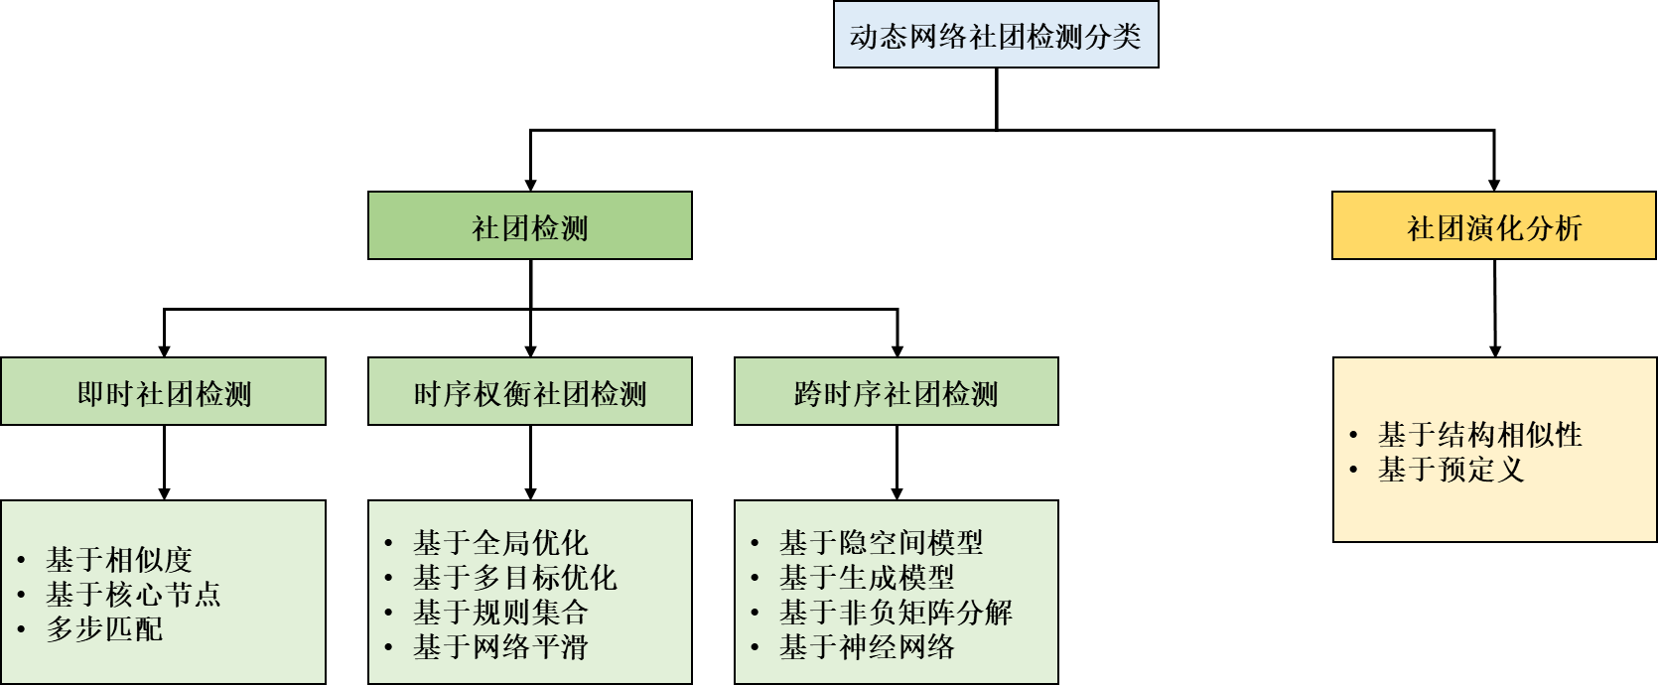
\includegraphics[width=.8\linewidth]{figures/chap01/classification of dcd.png}
    \caption{动态网络社团检测分类示意图}
    \label{chap1:fig:dcdclasses}
\end{figure}

\subsubsection{社团检测方法研究现状}

动态社团检测的任务核心仍然是识别每个网络快照的社团结构,根据模型对时序信息的融合思想,可以划分为即时社团检测、时序权衡社团检测与跨时序社团检测,其对时序信息的融合程度逐层递增,三类方法的优劣如表~\ref{chap1:dynamicmethod}所示。

\begin{table}[htbp]
	\caption{动态网络社团检测方法对比简表}
	\vspace{0.5em}\centering\wuhao
	\label{chap1:dynamicmethod}
	\resizebox{0.98\textwidth}{!}{
		\begin{tabular}{lp{4cm}p{3cm}p{3cm}cp{2cm}}
			\toprule[1.5pt]
			方法类别 & 核心思想 & 方法优势 & 方法不足 & 代表性工作\\
			\midrule[1.0pt]
			\textbf{即时社团检测} & 每个快照社团检测仅依赖于当前快照的网络结构,通过相似性进行跨时序社团匹配  & 可直接复用静态社团检测方法,易于并行计算,效率高 & 结果不稳定  & ~\cite{rosvall2010mapping,bota2011dynamic,falkowski2007data} \\
			\textbf{时序权衡社团检测} & 每个快照的社团结构依赖于前序快照的信息与当前快照网络拓扑 & 社团结果稳定,能够刻画社团及网络演化 & 难以并行,存在长时社团错误累积风险 & ~\cite{shang2014real,cazabet2011simulate,liu2020detecting} \\
			\textbf{跨时序社团检测} & 同时考虑所有快照进行社团检测 & 社团结果稳定,受噪声影响小 & 模型复杂度较高  & ~\cite{ma2019detecting,yang2011detecting,wilson2019modeling,de2021deep} \\
			\bottomrule[1.5pt]
		\end{tabular}
	}
\end{table}
\subsubsection{即时社团检测方法}
该方法的主要思想旨在基于已有成熟的静态网络社团检测方法与社团匹配方法实现对动态网络的社团检测,因此该方法并未考虑动态网络演化建模问题,此类方法属于典型的“两步法”,即首先对每个快照的网络运行静态社团检测方法以得到每个快照的社团结果,随后将相邻快照的社团进行对齐,以得到动态网络社团检测结果。此类方法按照匹配思想的区别可以划分成三类,分别是基于相似度的方法、基于核心节点的方法和基于多步匹配的方法,
% 各方法对比见表~\ref{chap1:tab:instantOptimal}。

% \begin{table}[htbp]
% 	\caption{即时社团检测方法分类对比简表}
% 	\vspace{0.5em}\centering\wuhao
% 	\label{chap1:tab:instantOptimal}
% 	\resizebox{0.98\textwidth}{!}{
% 		\begin{tabular}{lp{4cm}p{3cm}p{3cm}cp{2cm}}
% 			\toprule[1.5pt]
% 			方法类别 & 核心思想 & 方法优势 & 方法不足 & 代表性工作\\
% 			\midrule[1.0pt]
% 			\textbf{基于相似度的方法} & 各快照执行静态社团检测,通过相似度度量匹配相邻快照的社团 & 方法简单,运行效率高 & 无法识别社团演化行为  & ~\cite{palla2007quantifying,rosvall2010mapping,bota2011dynamic} \\
% 			\textbf{基于核心节点的方法} & 各快照执行静态社团检测,通过中心性高的节点的社团变化进行相邻快照社团匹配 & 方法简单,能够识别社团分裂、合并行为 & 识别效果相对不稳定 & ~\cite{wang2008commtracker,chen2010detecting} \\
% 			\textbf{基于多步匹配的方法} & 各快照执行静态社团检测,匹配社团时尽可能考虑多个连续快照的社团结果 & 社团检测效果较好,可以识别社团重现 & 无法处理在线数据  & ~\cite{falkowski2006mining,falkowski2007data} \\
% 			\bottomrule[1.5pt]
% 		\end{tabular}
% 	}
% \end{table}

基于相似度匹配的方法通过定义质量函数(如Jaccard相似度)来衡量不同快照的社团的相似程度,即相邻快照的两个社团如果相似度较高(或定义阈值),则认为这两个社团在连续快照中是同一个社团。Hopcroft等人\cite{hopcroft2004tracking}首先给出了基于相似度匹配的动态社团检测方法范式,首先通过同一个静态社团检测方法检测每个快照的社团结构,随后给出相邻快照中的社团匹配函数:
\begin{equation}
    match(C,C^{'})=min(\frac{\lvert C \cap C{'} \rvert}{\lvert C \rvert},\frac{\lvert C \cap C^{'} \rvert}{\lvert C^{'} \rvert}),
\end{equation}
其中$C$和$C^{'}$表示被匹配的两个社团内的节点集合。Pella等人\cite{palla2007quantifying}提出了以团渗透算法进行连续快照$t$到$t+1$的社团匹配,在该文章中,作者还探讨了如何利用社团内节点的变化来预估社团存续时长,他们观察到小型社团存续的关键在于对同质性节点的吸收能力,而大型社团存续的关键则在于持续的变化。Rosvall等人\cite{rosvall2010mapping}则考虑此类方法在大规模网络的应用问题,提出了在每个快照中寻找稳定社团的方法,即通过对原始网络的每个快照进行扰动以生成多个(具体来说,进行$1000$次扰动)新的网络,并重复进行社团检测,按照人工设置的阈值将这些社团结果进行合并进而形成稳定社团。在后续的工作中,Asur等人\cite{asur2009event}则提出了可以在社团匹配步骤中通过改进社团匹配函数来实现对动态网络社团演化行为的识别,并获得了一定发展\cite{bota2011dynamic}。

基于核心节点的方法则认为网络中具有较高权重的节点能够左右社团在时序的变化,因此在社团匹配过程中,如果相邻快照中的两个社团存在同一个中心性指标较高的节点,则这两个社团在连续快照中是同一个社团。这种方法相较于相似度匹配的方法能够识别社团的分裂或者合并行为,因为一个社团中可能存在多个核心节点,这些节点的社团转移并不一定相同。Wang等人\cite{wang2008commtracker}首先提出了此类方法的范式,并提出了一个投票策略来识别各个快照的社团中的核心节点。Chen等人\cite{chen2010detecting}在此基础上进行了优化,他们采用了社团的保守定义,即图中的最大团,来缩小社团匹配步骤的搜索域,提升效率的同时避免了冗余社团,并定义了代表社团的核心节点应该在同一快照中出现在其他社团频次最少。

多步匹配方法则并不仅考虑相邻快照的社团匹配,而是同时考虑多个相邻快照(尽可能远的)的社团匹配问题,匹配方法可以是基于相似度匹配或者基于核心节点的方法。此类方法能够识别社团重现,但难以实现在线运行,因为多步匹配可能在新快照加入后使得前序快照的社团结果发生改变。Falkowski等人\cite{falkowski2006mining,falkowski2007data}定义了多步匹配的核心思想,即根据社团相似性度量$overlap(x,y)=\frac{\lvert x \cap y \rvert}{min(\lvert x \rvert,\lvert y \rvert)}$将多个相邻快照中的相同社团进行关联,以得到社团存续图,随后在社团存续图中再次执行静态社团检测算法来获得多个快照的社团关联性。

即时社团检测的基本思想使得此类方法在识别社团结构时并不考虑时间信息对社团检测结果的影响,这使得此类方法受噪声影响较大,且社团检测结果不稳定,虽然以Rosvall等人\cite{rosvall2010mapping}为代表的部分学者利用策略获得稳定社团或通过缩紧社团定义以解决这些问题,但并未从本质上改变此类方法的短板。另外,此类方法在忽略社团检测效果的前提下,对于社团生命周期的检测也取得了一定的成果\cite{chen2010detecting},这也为社团演化分析任务提供了方法支撑。
\subsubsection{时序权衡社团检测方法}
此类方法考虑到了在动态社团检测任务中,前序快照对当前快照的影响,在进行当前快照社团检测时,需要权衡前序快照社团结构与网络演化对当前快照社团检测的影响,但并不考虑未来快照对当前快照的影响,这也是此类方法能够实现在线社团检测的前提,称为进化聚类。此类方法可以总结为两个迭代步骤,首先对动态网络第一个快照的网络执行社团检测,随后对后续快照按时序在结合前序快照社团结构的前提下逐个识别社团结构。按照方法的不同,此类方法可以进一步划分成基于全局优化、基于多目标优化、基于规则集合和基于网络平滑的方法。基于全局优化和基于多目标优化的方法主要基于前序快照的社团结构与当前快照与前一快照的网络图谱变化来更新社团结果;而基于规则集合和基于网络平滑的方法则在对当前快照进行社团检测时考虑前序快照的信息。
% 各方法对比见表~\ref{chap1:tab:instantOptimal}。

% \begin{table}[htbp]
% 	\caption{即时社团检测方法分类对比简表}
% 	\vspace{0.5em}\centering\wuhao
% 	\label{chap1:tab:instantOptimal}
% 	\resizebox{0.98\textwidth}{!}{
% 		\begin{tabular}{lp{4cm}p{3cm}p{3cm}cp{2cm}}
% 			\toprule[1.5pt]
% 			方法类别 & 核心思想 & 方法优势 & 方法不足 & 代表性工作\\
% 			\midrule[1.0pt]
% 			\textbf{基于全局优化的方法} & 各快照执行静态社团检测,通过相似度度量匹配相邻快照的社团 & 方法简单,运行效率高 & 无法识别社团演化行为  & ~\cite{palla2007quantifying,rosvall2010mapping,bota2011dynamic} \\
% 			\textbf{基于规则集合的方法} & 各快照执行静态社团检测,通过中心性高的节点的社团变化进行相邻快照社团匹配 & 方法简单,能够识别社团分裂、合并行为 & 识别效果相对不稳定 & ~\cite{wang2008commtracker,chen2010detecting} \\
% 			\textbf{基于多目标优化的方法} & 各快照执行静态社团检测,匹配社团时尽可能考虑多个连续快照的社团结果 & 社团检测效果较好,可以识别社团重现 & 无法处理在线数据  & ~\cite{falkowski2006mining,falkowski2007data} \\
% 			\bottomrule[1.5pt]
% 		\end{tabular}
% 	}
% \end{table}
基于全局优化的方法主要以社团聚类质量函数为衡量指标(如模块度、传导率等),以$t$时刻的社团检测结果为起点,迭代地将$t+1$时刻的节点更换社团归属以最大化质量函数,从而达到识别$t+1$时刻社团的目的。Miller等人\cite{miller2010continuous}参考潜在狄利克雷分配过程(Latent Dirichlet Allocation,LDA)设计了动态图主题模型,将社团视作随时序演化的主题,节点之间的连边则对应文档中的词汇,通过前一个快照的主题来初始化当前快照的主题,通过这种方法实现了对动态网络时序演化的建模与社团检测。Aynaud等人则利用模块度优化方法来实现对动态网络社团演化的建模,首先在第一个快照上运行Louvain算法识别其社团结构,随后通过在后续快照中改变节点的社团划分来优化模块度,使模块度达到局部最优,为了保证社团稳定性,$t$时刻的社团结构初始化由$t-1$时刻确定。G{\"o}rke等人\cite{gorke2010modularity}在社团初始化设置的基础上添加了回溯策略以提升$t$时刻社团的搜索空间。Shang等人\cite{shang2014real}则进一步提出了在动态社团检测过程中,在对$t$时刻快照进行社团检测之前,引入网络修剪策略来尽可能将$t$时刻的网络结构的拓扑噪声进行剔除。  

基于规则集合的方法考虑在前序快照和当前快照之间发生的网络变化(边/节点的出现或消失),定义一系列规则来确定网络变化如何更新当前快照的社团。Falkowski等人\cite{falkowski2008studying}基于经典的DBSCAN\cite{10486339}方法提出了DENGRAPH算法,该方法定义了一个新的临近性指标,其定义了节点对之间的距离。当节点$u$和$v$的临近性超过阈值时,称节点$u$和$v$密度可达。当节点$u$具有超过$\eta$个密度可达邻居时,则称$u$为核心节点。社团由密度可达的核心节点的集合组成。通过定义上述规则,该算法可以根据动态网络快照的节点和边的变化快速更新动态网络社团结构,其社团定义较一般社团的定义更为严格。Nguyen等人\cite{nguyen2011adaptive}则提出了QCA算法,设计一系列的规则函数来根据动态网络前一个快照的网络结构变化(节点/边的添加和消失)更新当前快照的社团划分。Cazabet和Amblard\cite{cazabet2011simulate}则从强化学习的角度提出了基于多agent的社团检测方法,其将动态网络视作环境变量、社团视作环境中的agent,当环境发生改变,则通过策略集中定义的规则对社团结果进行更新。

基于多目标优化的方法则同时考虑了当前社团检测效果与当前快照和前序快照之间的时序平滑性,因此其定义了优化范式来融合两个优化目标:
\begin{equation}
c=\alpha CS+(1-\alpha CT),
\end{equation}
其中$CS$表示当前快照的社团检测效果,$CT$表示时序平滑性效果,$\alpha$则表示二者的权重。Zhou等人\cite{zhou2007discovering}首先提出基于正则化割是被每个快照的社团,并引入额外的距离函数衡量当前快照社团划分与前序快照社团划分之间的差距,通过多目标优化范式平衡当前社团结果与前序社团结果的最优化以获得动态网络社团结果。Folino等人\cite{folino2013evolutionary}在多目标优化框架下引入了遗传算法,第一个目标函数用来提升当前快照的社团检测结果,第二个目标通过最大化当前快照与前一快照的正则化标准互信息(Normalized Mutual Information,NMI)来确保网络平滑性。Sun等人\cite{sun2013co}通过狄利克雷过程混合模型实现对动态网络的社团生成,利用吉布斯采样对模型参数进行推断求解,其社团发现由当前快照的最优社团与前序快照的演化平滑之间进行平衡。Liu等人\cite{liu2020detecting}考虑动态网络社团演化行为的变化引入了社团迁移操作符来细化动态网络社团演化模式。

基于网络平滑的方法则通过考虑过去网络的变化来优化当前快照的网络拓扑,例如按照前序网络变化来对当前快照的网络结构增加或删除边,以此将网络平滑性融入到当前快照中,进一步在平滑后的当前快照中执行社团检测算法。Guo等人\cite{guo2014evolutionary}基于模块度优化方法设计了基于网络平滑的动态网络社团检测算法,其对当前快照的网络结构与前一快照的网络结构进行融合,形成trade-off邻接矩阵,并在该邻接矩阵中进行静态社团检测以获得动态社团划分结果。Xu等人\cite{xu2013community}则设计了更加精细的更新策略,通过设计\textit{累积稳定边}来得到动态网络演化过程中相对稳定的结构,并在此结构上进行社团检测,以此获得稳定的动态社团划分。

时序权衡社团检测方法通过不同的设计思路来平衡各快照的最优社团结果与时序平滑性对动态社团检测的影响。此类方法由于考虑了时序平滑性,因此能够产生在时序过程中稳定的社团结果。但由于对动态网络每个快照进行社团检测时需要考虑前序快照或多个前序快照的信息,因此此类方法难以并行计算。另外,由于对动态网络时序平滑的引入,此类方法可能存在社团结果的错误累积,导致长时间序列的动态网络社团检测结果逐渐失真。

\subsubsection{跨时序社团检测方法}
此类方法将动态网络的演化建模与动态社团检测进行融合,以获得更加全局的动态网络社团检测结果。此类方法的社团检测效果主要取决于对于动态网络演化建模的有效程度,也是当前动态社团检测的主流思想。此类方法按照方法不同可以划分为基于非负矩阵分解的方法、基于隐空间模型的方法、基于生成模型的方法和基于神经网络的方法。

非负矩阵分解方法进行社团检测的核心思想是利用非负矩阵对网络拓扑的低维分解等价于聚类方法的原理,通过设计模型将动态网络演化模式融入到模型中以达到对动态网络演化建模及社团检测的目的\cite{KXTS202104002}。Lin等人\cite{lin2009analyzing}提出的FacetNet算法,在$t$时刻的社团检测通过引入混合模型来实现,而对于动态网络平滑则通过计算当前快照与前序快照的KL散度实现,提升了模型的鲁棒性。而FacetNet通过非负矩阵分解的技术路线将网络演化与社团检测进行了联合建模。Gao等人\cite{gao2017dynamic}提出的ENMF则参考动态随机块模型(Dynamic Stochastic Block Model,DSBM)\cite{yang2011detecting}引入了社团转移矩阵来显式地刻画动态网络的演化,可以在保证社团检测效果的前提下支持动态网络演化分析。Ma等人\cite{ma2017evolutionary}则证明了ENMF与动态谱聚类方法在理论上是等价的,并基于该证明将谱聚类引入到ENMF框架中,提升了该模型的社团检测效果。Ma等人\cite{ma2019detecting}在后续工作中进一步引入了图正则项将动态网络历史快照的结构融入到当前快照社团检测任务中,在保证复杂度不增的前提下进一步提升了社团检测效果。

隐空间模型则认为复杂网络的演化受到高维空间的影响,因此可以通过将动态网络的节点或边组成的拓扑结构映射到高维空间中,并在高维空间建模动态网络的演化。在此过程中将社团结构融入到模型中来同步获得动态网络社团划分。Sewell等人\cite{sewell2015latent}首先提出了动态隐空间模型的范式,即通过将节点映射到高维隐空间中来表示节点在网络中的位置(类似于网络表示学习),并利用节点高维空间相似性聚类实现社团检测,并利用隐马尔可夫模型建模社团在高维隐空间中的演化模式,随后利用MCMC采样实现对社团求解。Liu等人\cite{liu2022variational}则引入了变分推断的方法来对隐空间模型参数进行求解,提升了模型的运行效率。Daniel等人\cite{daniel2023bayesian}则针对动态隐空间模型在高维空间中的时序演化机制进行了细化,通过引入层次狄利克雷隐马尔可夫模型显式地建模了社团的分裂合并等行为。

生成模型则在隐空间模型的概念上更进一步,通过设计动态网络的生成机制,并将社团结构纳入到生成机制中(即认为动态网络的节点和边的生成及演化受到社团的影响),通过对该生成机制的模型参数求解以获得动态网络社团划分。其中最经典的方法是Yang等人\cite{yang2011detecting}提出的动态随机块模型DSBM,该模型通过引入社团转移矩阵来显式地建模了动态网络社团的演化,并沿用了经典随机块模型的网络生成机制,即节点的连边仅与节点所在社团有关。在此基础上进一步提出假设,节点的社团划分的演化仅与其所在社团与社团转移矩阵有关。DSBM提出了模型参数的两种推断方法,分别是基于共轭先验的参数后验推断与EM算法,并给出了在线和离线两个版本的模型。Tang等人\cite{tang2014detecting}在此基础上考虑DSBM无法实现动态社团模型选择的问题,提出了基于狄利克雷过程的动态随机块模型,通过狄利克雷过程自动确定动态网络社团个数。Xu\cite{xu2015stochastic}则对DSBM的演化所依赖的隐马尔可夫假设进行了改进,允许前序边的变化直接影响当前快照边的生成,并提出了结合卡尔曼滤波和局部搜索的求解策略。Wilson等人\cite{wilson2019modeling}引入了度异质性参数来对DSBM进行了改进,实现了随机块模型对节点的度异质性进行捕获。

基于神经网络的方法则普遍将动态网络建模与社团检测任务切分开来,利用图神经网络将动态网络各快照中的拓扑与属性信息进行解耦,形成节点的低维表示,并在节点表示向量中利用聚类算法获得社团结构,代表性的方法包括基于GCN的方法\cite{ma2020streaming,pareja2020evolvegcn}、基于GAT的方法\cite{cui2019hierarchical}、基于AE的方法\cite{goyal2018dyngem,yu2018netwalk,zhao2019large,goyal2020dyngraph2vec}等。上述方法的创新点均是为了模型能够更好地捕获动态网络的属性或拓扑信息以获得节点的表示向量,而执行社团检测任务往往通过对节点表示向量执行聚类操作实现,这种“两步法”的方式虽然效率较高,但所获得的聚类结果本质上是相似节点的集合,并不能直接代表动态网络的社团结构。Santo等人\cite{de2021deep}则通过基于CNN的稀疏卷积设计,同时引入部分社团真相实现了对动态网络社团的半监督学习,但社团本质是无监督任务,引入社团真相一定意义上无法在实际应用中起到作用。Yao等人\cite{yao2021interpretable}则通过改进动态网络快照的网络结构,引入衰减参数将前序快照与当前快照网络结构进行融合,通过神经网络学习网络表示,并引入谱聚类获得社团结构,该方法还证明了此种改进理论上与DSBM近似。由于神经网络属于经典的黑盒模型,即使其针对动态社团检测任务进行了优化,模型参数也无法理解,难以应用到社团演化分析任务中。

跨时序社团检测方法的核心是更好地实现动态网络演化模式的建模,因此此类方法往往能够适应更多的动态网络下游任务,如链接预测、异常检测、演化分析等。并且此类方法中,生成模型、隐空间模型及非负矩阵分解方法的模型隐变量均具备一定的物理或现实意义,故其具有良好的可解释性,其中以生成模型的可解释性最好,能够支撑更深入的网络演化分析及挖掘任务,但往往复杂的模型架构与模型推断复杂导致上述模型难以适用于大规模网络。而基于神经网络的方法往往由于其黑盒特性而缺乏可解释性,因此难以用于社团演化分析研究。




\subsubsection{社团演化分析研究现状}

社团演化分析任务的核心是通过挖掘动态网络社团随时间的变化模式,以揭示社团结构的时序演化规律,支持人们对复杂系统的因果关系理解与推断、预测以及控制。对社团演化的分析可以帮助提升复杂系统的鲁棒性与韧性。动态网络社团演化分析的相关方法按照设计思路可以划分为基于结构相似性的方法和基于预定义的方法。方法对比见表~\ref{chap1:tab:ievolution}

\begin{table}[htbp]
	\caption{社团演化分析方法分类对比简表}
	\vspace{0.5em}\centering\wuhao
	\label{chap1:tab:ievolution}
	\resizebox{0.98\textwidth}{!}{
		\begin{tabular}{lp{4cm}p{3cm}p{3cm}cp{2cm}}
			\toprule[1.5pt]
			方法类别 & 核心思想 & 方法优势 & 方法不足 & 代表性工作\\
			\midrule[1.0pt]
			\textbf{基于结构相似性的方法} &通过定义相邻快照的相似性指标来识别社团的时序演化关系 & 指标相对直观,易于理解 & 泛化能力差,可解释性较差  & ~\cite{palla2007quantifying,zhong2014evolution,wang2024community} \\
			\textbf{基于预定义的方法} & 通过预定义动态网络中的演化事件,并定义阈值来进行动态网络事件检测 & 扩展性强,理解直观,可帮助预测社团未来行为 & 依赖人工定义的指标,缺乏统一标准 & ~\cite{greene2010tracking,brodka2013ged,mazza2023modularity,zhao2023dynamic} \\
			\bottomrule[1.5pt]
		\end{tabular}
	}
\end{table}
\subsubsection{基于结构相似性的方法}
此类方法的基本假设认为动态网络每个快照的社团结构已经获得,通过定义相邻快照的相似性指标并定义阈值来识别社团在时序上的演化关系,进而分析社团的演化模式。Palla等人\cite{palla2007quantifying}通过团渗透的方法获得了动态网络的社团结构,进而定义了社团在不同快照中的自相关函数以及社团稳定性指标,通过对论文合作网络与通信网络的分析,得到不同规模社团的演化规律,即大规模社团变动频繁、小规模社团相对稳定。Zhang等人\cite{zhong2014evolution}针对物联网网络的演化,提出了基于模块度增益的社团演化分析方法,并引入了正则化互信息指标与自相关函数来衡量社团稳定性。Wang等人\cite{wang2024community}考虑物理系统的鲁棒性,通过定义广义介数中心性模型与网络负荷流模型来模拟通信网络和电力网络在演化过程中的鲁棒性,该模型考虑了社团结构在网络演化中的作用,并总结出社团边缘的节点变动对网络鲁棒性影响较大。
基于结构相似性的方法以定义网络演化相似性度量实现对动态网络与动态社团演化的建模与分析,这种方式依赖于指标设计与社团检测效果,且其模型往往缺乏可解释性,不具备指标外的泛化能力。

\subsubsection{基于预定义的方法}
此类方法将社团演化行为视为网络中的各种事件,通过识别网络中的预定义事件的模式来分析动态网络及动态社团的演化。Greene等人\cite{greene2010tracking}提出了一种可扩展的社团演化事件识别方法,通过定义社团诞生、死亡、合并、分裂、扩展、收缩事件,并设计一系列阈值进行匹配来实现对社团演化事件的识别。Br{\'o}dka等人\cite{brodka2013ged}则进一步将社团演化事件扩展成$8$种,并定义了社团归属指标$I$来衡量两个社团的相似性,基于该指标进一步定义了一系列的阈值进行社团演化事件的识别。Mazza等人\cite{mazza2023modularity}则提出了无阈值框架,通过将所识别的社团结构视为节点,社团间的相似性视为边构建了社团相似性网络,并在该网络中进行模块度优化聚类,用聚类结果实现动态网络社团演化分析。Zhao等人\cite{zhao2023dynamic}则在考虑人类移动的空间平滑性更新了上述社团演化事件的定义,并将其应用在城市人类移动分析中。
基于预定义的方法以预定义的事件及事件特征为基准,通过设定阈值识别网络中的事件,对动态网络及动态社团的演化分析比较直观,但且缺乏统一标准,需要人工信息指导。

总的来说,动态网络社团演化分析方法往往依赖于社团检测准确性,难以完全脱离动态社团检测任务而独立存在。

\section{研究内容与创新点}

本文以动态复杂网络为研究对象,从动态网络社团检测与演化分析任务出发,重点关注动态网络的生成机制建模与分析,从随机块模型的角度构建动态网络的高阶生成机理,从实证分析出发,解决生成模型在动态网络演化机制中的社团与节点的演化异质性缺失问题,以提升随机块模型对动态网络演化模式的建模能力与演化分析能力,并结合图神经网络与深度序列模型探索了动态社团检测的深度生成建模方法,为动态社团检测的大规模数据可解释性建模提供基础。
从研究目标上,以随机块模型为理论基础,针对真实世界动态网络数据挖掘动态网络的高阶生成机理,支撑动态网络演化模式改进;提出动态网络的微观节点-介观社团-宏观网络快照的层次狄利克雷生成框架,扩展动态随机块模型的网络高阶生成机理建模能力;从动态随机块模型的动态网络演化分析提升出发,提出动态网络层次演化异常识别指标,扩展动态随机块模型的动态网络演化分析深度;针对高精度动态随机块模型参数量过高,难以针对大规模数据扩展问题,提出动态网络深度生成模型社团检测建模,解决深度学习模型的黑盒问题同时,为动态网络生成模型的大规模应用提供方法框架。其研究思路及主要研究内容关系如图~\ref{chap1:fig:framework}所示:

\begin{figure}[htbp]
    \centering
    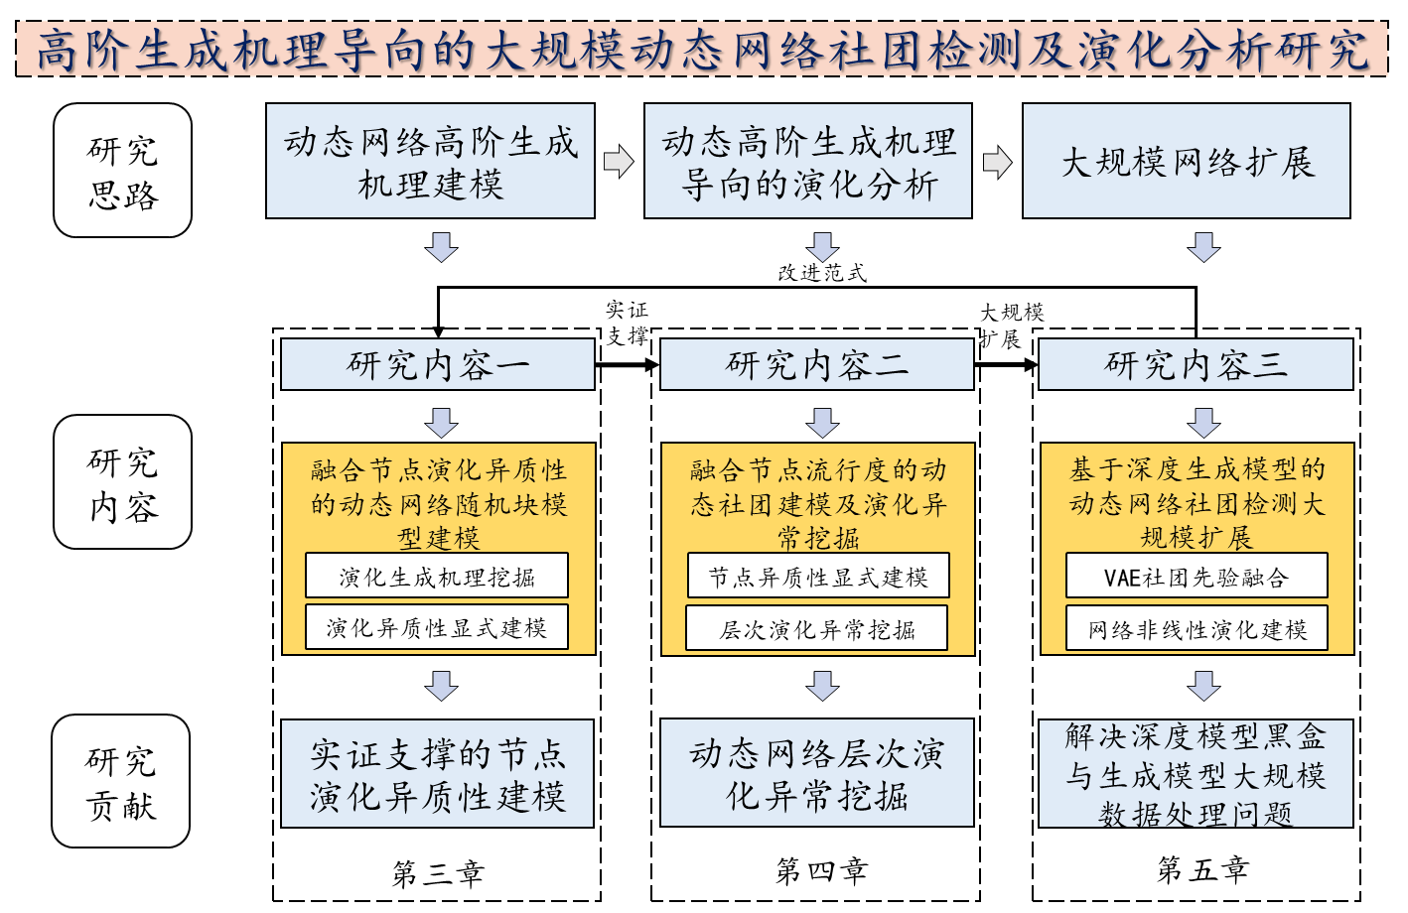
\includegraphics[width=.9\linewidth]{figures/chap01/framework.png}
    \caption{本文研究思路及关联}
    \label{chap1:fig:framework}
\end{figure}

第一,提出动态网络高阶生成机理挖掘框架,探索动态网络节点变化与社团演化之间的本质关联。考虑到动态网络的演化由节点和边的变化驱动,而社团的演化则由节点的社团归属变化而驱动,因此需要明确动态网络中节点演化与社团演化的相互作用关系。在其指导下,研究融合动态网络高阶生成模式的动态随机块模型。针对经典随机块模型对动态网络生成机理建模能力提升的问题,设计生成机制,进一步地提升动态随机块模型的建模能力,并研究有效的动态随机块模型参数推断方法,进而验证该模型在社团检测与社团演化分析的有效性。

第二,研究动态随机块模型社团演化分析的深入挖掘方法。在研究内容一的基础上,改进并简化动态随机块模型的建模方法,提升模型参数的可解释性与易理解性,研究基于动态随机块模型的动态网络各层次演化异常定义以提升动态随机块模型的社团演化分析能力,并验证其有效性。

第三,针对动态随机块模型难以大规模应用问题,研究基于深度学习的动态社团深度生成建模方法。以生成模型为出发点,基于深度生成模型的框架研究生成模型参数的变分自编码器求解方法,并验证模型的动态社团检测能力及其参数的动态社团演化分析能力与大规模数据应用能力。

针对以上研究内容,本文从动态网络演化建模的角度,深入分析并提出了解决方法,取得了一定研究成果,并通过实证分析验证了提出方法的贡献。其主要贡献和创新点包括一下几个方面:

第一,本文采用特征工程的方法,将动态网络节点的社团转移行为定义成相邻快照节点是否转移的二分类问题,并提取动态网络各快照中节点与社团的属性信息,基于决策树分类实现对节点在动态网络演化过程中的高阶生成机制挖掘,通过收集大量真实世界动态网络数据进行横向对比,应用不同的经典社团检测方法剔除社团检测方法的纵向影响,定性挖掘动态网络高阶生成机理,为后续模型设计提供了实证依据。

第二,在研究内容一的支撑下,本文提出建模动态网络节点-社团演化机制的层次狄利克雷生成结构,基于动态随机块模型的基本假设,进一步引入节点级别的社团转移参数,并定义了社团转移参数与节点级别的社团转移参数的生成关系以建模动态网络的高阶演化机制。通过变分推断方法对所提出模型进行参数后验推断,以估计模型参数拟合结果。通过在生成数据集与真实数据集的社团检测、社团演化与节点演化实验,验证了所提出方法对网络高阶生成机理建模的有效性和可行性,并挖掘了论文引用网络中节点与社团演化的规律。

第三,考虑到动态随机块模型对网络生成机制的显式建模能力,本文提出了融合节点流行度的动态随机块模型以同时建模节点拓扑异质性与演化异质性,根据该模型参数和隐变量的实际意义提出了面向微观节点、介观社团以及宏观网络快照的演化异常识别指标,拓展模型的动态网络演化分析能力,通过对真实世界数据的实验验证了本模型对动态网络及动态社团的建模能力与所提出的动态网络层次演化异常指标的有效性。

第四,针对生成模型对动态网络生成及演化的可解释性建模能力强但高精度模型参数量大、参数依赖关系复杂、模型求解难得问题,以及动态网络深度模型建模相对简单且运行效率高(易于优化)但黑盒特性限制其对真实世界动态网络演化分析能力的问题,提出结合二者优势的深度生成模型,利用变分自编码器与生成模型变分推断求解的理论关联,提出融合混合高斯先验的基于变分自编码器的动态网络深度社团检测算法,利用深度序列模型建模动态网络的非线性演化。针对生成数据集与真实数据集的实验验证了所提出方法的有效性以及基于深度生成模型的动态网络演化模式挖掘的可行性,为后续动态网络社团检测算法的推广与应用提供了有效的建模框架。

\section{论文组织结构}
本文对动态社团生成机制及其深度建模问题展开研究并提出了三个工作,全文的章节结构如下所示:



第一章,主要介绍了动态网络社团检测的研究背景和意义,指出了本文的研究问题,分析了当前国内外的研究现状和挑战,随后对本文研究内容进行阐述。

第二章,介绍了本文的相关研究基础,包括动态网络社团检测相关研究技术与前沿方法,包括其研究思路以及优缺点,进一步介绍了基于深度学习的动态网络社团检测方法的相关技术路线以及深度生成模型的相关基础。

第三章,针对动态网络社团演化与节点演化的关联性设计研究框架,利用大量真实世界数据进行动态网络高阶生成机理的规律挖掘,并在此实证基础上提出融合节点演化异质性的动态随机块模型,随后介绍了模型的变分推断估计方法与实验结果及实证分析。

第四章,针对动态随机块模型的演化分析能力提升,首先提出融合节点流行度的动态随机块模型以提升模型的可解释性,随后介绍基于模型参数的动态网络、社团、节点的各层次演化异常指标,最后介绍实验以验证模型与所定义指标的有效性并进行实证分析。

第五章,针对生成模型可解释性强但模型推断复杂难以应用于大规模数据,以及基于深度模型的方法可解释性差但方法设计简单且运行效率高的特点,提出了基于深度生成模型的动态网络深度社团检测算法,随后介绍模型实验以验证所提出方法能够融合深度模型与生成模型的优势,验证了所提出方法在动态网络演化分析的应用潜力。

第六章,总结与展望,对本文的工作和贡献进行了总结,并展望未来动态网络社团检测及演化分析的研究思路。




% !Mode:: "TeX:UTF-8"
\baselineskip 20pt

%-------------------------------------------------------------------------
\chapter{相关研究基础}
\label{chap:2}
本章从方法论的角度首先将当前主流的动态网络社团检测相关方法划分为基于启发式优化的方法、基于模块度优化的方法、基于矩阵分解的方法、基于谱优化的方法、基于多目标优化的方法、基于随机块模型的方法和基于深度学习的方法。并介绍与本文相关的深度生成模型研究基础。为了验证动态社团检测方法的有效性,本章还介绍了用于衡量动态社团检测效果的常用评价指标。

\section{动态网络社团检测相关研究}
动态网络的社团检测的核心任务是识别网络中每个快照的社团结构,这需要考虑动态网络及动态社团的演化建模,大量的研究人员围绕着动态网络的演化建模以及动态社团检测从不同技术路线进行创新~\cite{JSJA2023S2059},其中主要的方法可以划分为基于启发式优化的方法、基于模块度优化的方法、基于矩阵分解的方法、基于谱优化的方法、基于多目标优化的方法、基于随机块模型的方法和基于深度学习的方法。各方法的优劣势及原理对比见表~\ref{chap2:tab:community}。需要注意的是,各类方法的设计思路往往并不局限于动态网络建模的某一个思路如即时社团检测。


\subsection{基于启发式优化的方法}
动态网络社团检测基于启发式优化的方法思路较朴素,即根据动态网络社团的基本定义,通过设计优化目标,再利用贪婪搜索或极值优化的方法对优化目标的解空间进行求解。

Tant等人\cite{tantipathananandh2007framework}首先根据社团的基本定义与动态网络的特性提出动态社团的启发式优化方法,该方法首先定义动态社团演化的假设,即动态网络中的节点更倾向于不频繁更换其社团归属,且大多数时间都倾向于与同一社团内的其他节点进行交互,随后证明了动态社团检测属于NP-hard完全问题,最后提出将动态社团检测分解成两个子问题,并提出基于动态规划和贪婪启发式优化的求解方法。

\begin{table}[H]
	\caption{动态社团检测各技术路线方法对比简表}
	\vspace{0.5em}\centering\wuhao
	\label{chap2:tab:community}
	\resizebox{0.98\textwidth}{!}{
		\begin{tabular}{p{2cm}p{4.2cm}p{3cm}p{4.8cm}cp{2cm}}
			\toprule[1.5pt]
			方法类别 & 核心思想 & 方法优势 & 方法不足 & 代表性工作\\
			\midrule[1.0pt]
			\textbf{基于启发式优化的方法} & 根据社团的概念定义优化指标,利用各种优化方法解决社团检测的NP-hard问题& 易于获得较好的局部最优解,指标定义符合直觉,易于理解 & 依赖指标定义,需要全局搜索,不具备可解释性,难以应用到社团演化分析中,模型复杂 & ~\cite{kawadia2012sequential,kauffman2014dyconet,sarzynska2016null,10452807} \\
			\textbf{基于矩阵分解的方法} & 基于非负矩阵分解技术,首先对动态网络进行建模,并将社团结构融入到矩阵分解架构中进行求解 & 有理论支撑,且易于扩展,能够应用与多种下游任务 & 模型随这动态网络规模增长,时间与空间复杂度均呈平方或指数增长,难以适用于大规模数据 & ~\cite{wang2010low,li2021detecting,li2021identification} \\
			\textbf{基于谱优化的方法} & 基于谱图理论支撑,通过谱优化操作将过滤网络噪声,提升动态社团检测的效果 & 理论完善,对噪声的适应能力较强 & 谱图理论难以保证动态网络的演化建模,需要额外的设计& ~\cite{xu2014adaptive,langone2016efficient,karaaslanli2020constrained} \\
			\textbf{基于多目标优化的方法} & 通过平衡社团检测效果与网络平滑性两个优化目标的权重达到融合社团检测与社团演化建模的目的 &有效建模了网络动态平滑性 & 缺乏可解释性,多优化目标权重需要额外的测试确定,无法显式建模动态网络演化 & ~\cite{folino2013evolutionary,niu2017label,su2021parallel} \\
			\textbf{基于动力学的方法} & 通过随机游走或标签传播技术,根据社团结构特性在动力学过程中实现社团结构获取 & 运行效率高,易于并行 & 模型不稳定,获得的社团结果准确性差,难以支撑社团演化分析 & ~\cite{xie2013labelrankt,han2017community,xin2016adaptive,doi:10.1126/sciadv.abj3063} \\
			\textbf{基于随机块模型的方法} & 基于概率图模型设计动态网络的演化机制,并将社团结构融入到模型中,利用统计推断方法求解模型参数后验 & 模型可解释性强,扩展性强,能够适用于多种下游任务,能够有效地支撑动态网络及动态社团演化分析 & 模型建模精度越高,参数量越多,难以适用于大规模数据,且模型求解方法复杂 & ~\cite{yang2011detecting,xu2014dynamic,riverain2023poisson} \\
			\textbf{基于深度学习的方法} & 通过图神经网络首先学习动态网络的表示,通过对节点表示进行聚类获得社团结构(或同时建模社团结构) & 模型运行效率较高,能够适应于大规模数据,且模型架构设计方便,易于更新迭代 & 属于“黑盒”模型,参数不具备解释性,难以应用于动态网络演化分析 & ~\cite{goyal2020dyngraph2vec,hajiramezanali2019variational,mrabah2019deep} \\
			\bottomrule[1.5pt]
		\end{tabular}
	}
\end{table}

Tant等人后续针对该方法又进一步提出了扩展,从求解方式上提出将全局搜索问题转化为常因子近似问题并证明了其近似算法以概率$1$收敛到最优解\cite{tantipathananandh2009constant};从适用范围扩展到加权、有向网络的动态社团检测上\cite{tantipathananandh2011finding}。Kauffman等人\cite{kauffman2014dyconet}则根据即时社团检测的范式对该方法提出了改进,首先利用Louvain算法进行社团划分,随后利用Jaccard相似性进行社团匹配。Kawadia等人\cite{kawadia2012sequential}则根据相邻快照中的社团结构应尽可能保持一致的观点定义了快照间社团相似性指标(Estrangement Confinement,EC),将动态网络社团匹配问题转化成一个带约束的凸优化问题进行求解得到社团结构。

基于启发式优化方法的经典方法是模块度优化方法,模块度\cite{newman2004finding}的定义为:
\begin{equation}
	Q = \frac{1}{2m} \sum_{ij} \left[ A_{ij} - \frac{k_i k_j}{2m} \right] \delta(c_i, c_j),
\end{equation}

\noindent其中,\( m \) 是网络中边的总数,即 \( m = \frac{1}{2} \sum_{ij} A_{ij} \);\( A_{ij} \) 是网络邻接矩阵的元素,若节点 \( i \) 和 \( j \) 之间有边,则 \( A_{ij} = 1 \),否则 \( A_{ij} = 0 \);\( k_i \) 和 \( k_j \) 分别是节点 \( i \) 和 \( j \) 的度;\( \frac{k_i k_j}{2m} \) 表示在随机网络(空模型)中,节点 \( i \) 和 \( j \) 之间预期的边数;\( \delta(c_i, c_j) \) 是一个指示函数,若节点 \( i \) 和 \( j \) 属于同一社团(即 \( c_i = c_j \)),则 \( \delta(c_i, c_j) = 1 \);否则 \( \delta(c_i, c_j) = 0 \)。
模块度 \( Q \) 从直观上定义了网络中节点的聚集性,因此模块度越高则社团连接越紧密。He等人\cite{he2015fast}提出了基于模块度优化的动态网络社团检测算法,其优化思路如下:首先在第\(1\)个快照中运行静态模块度优化算法,随后在$t \ge 2$快照中,根据快照$t$与快照$t-1$的拓扑结构差异,将同一社团内连边没有变化的节点视作一个节点以构成新网络,再进行静态模块度优化社团检测,迭代更新得到动态网络的模块度优化社团检测方法。Nguyen等人\cite{nguyen2011adaptive}则简化了上述流程,通过对比快照$t$与快照$t-1$的节点和边的变化,增量更新模块度增益,并通过贪婪法或动态规划法求解社团结构。G{\"o}rke等人\cite{gorke2013dynamic}则在此基础上进一步提出改进,在此基础上融入动态网络平滑性指标,通过二者的权衡进行优化,实现了对社团平滑性演化的建模。J.Mucha等人\cite{mucha2010community}则认为模块度概念并不完全适用于动态网络社团检测,因此提出了针对动态网络的模块度概念,其定义为:
\begin{equation}
	Q_{\text{dynamic}} = \frac{1}{2M} \sum_{t=1}^{T} \sum_{ij} \left[ A_{ij}^{(t)} - \gamma_t \frac{k_i^{(t)} k_j^{(t)}}{2m^{(t)}} \right] \delta(c_i^{(t)}, c_j^{(t)}) + \sum_{t=1}^{T-1} \sum_{i} J_{i}^{(t, t+1)} \delta(c_i^{(t)}, c_i^{(t+1)}),
\end{equation}
\noindent其中,\( T \) 指网络快照的个数;\( M = \sum_{t=1}^{T} m^{(t)} \) 是所有快照中边的总数,\( m^{(t)} = \frac{1}{2} \sum_{ij} A_{ij}^{(t)} \) 是快照 \( t \) 的边数;\( A_{ij}^{(t)} \) 是快照 \( t \) 的邻接矩阵元素;\( k_i^{(t)} \) 和 \( k_j^{(t)} \) 分别是节点 \( i \) 和 \( j \) 在快照 \( t \) 的度;\( \gamma_t \) 是快照 \( t \) 的分辨率参数,用于调整社团大小的偏好,动态网络中通常设置为$1$;\( \frac{k_i^{(t)} k_j^{(t)}}{2m^{(t)}} \) 表示快照 \( t \) 在随机网络中节点 \( i \) 和 \( j \) 之间的预期边数(空模型);\( \delta(c_i^{(t)}, c_j^{(t)}) \) 是快照\( t \) 的社团指示函数,若节点 \( i \) 和 \( j \) 在时间 \( t \) 属于同一社团,则为$1$,否则为$0$;\( J_{i}^{(t, t+1)} \) 是时序耦合参数,表示节点 \( i \) 在 \( t \) 和 \( t+1 \) 之间的连接强度,可以用来控制相邻快照间的耦合性。通过优化动态模块度指标,可以同时得到动态网络中每个快照的社团结构,是一种离线的优化方法\cite{sarzynska2016null,10452807}。

总体上看,基于启发式优化的方法通常是根据社团和动态社团的基本概念或特征,定义对应的优化指标,根据指标进行启发式的优化以得到动态网络的社团检测结果。该方法的优化往往利用极值优化、贪婪优化或动态规划的方法,因此往往能够获得较好的局部最优解,但模型效率不高。由于其过于依赖指标的定义,因此社团检测结果往往依赖于所定义指标的优劣,结果不稳定,且其对于动态网络的演化建模往往是依据直觉,难以应用于社团演化分析任务中。



\subsection{基于矩阵分解的方法}
基于矩阵分解的动态网络社团检测方法建立在非负矩阵分解的理论基础上,可以通过将动态网络快照的邻接矩阵进行分解以得到社团结构,其可以通过学习局部特征而实现社团检测\cite{lee1999learning}。而根据复杂网络的稀疏性与社团的弱监督或无监督性,不同的矩阵分解方法陆续被提出,如图正则NMF\cite{cai2010graph}、弱监督NMF\cite{choo2015weakly}等。由于基于矩阵分解的方法一定意义上提供了网络的生成和演化机制的建模,因此其具备一定的可解释性和泛用性,在链接预测\cite{ma2017nonnegative}等任务都有一定应用。

在动态网络中,Wang等人\cite{wang2010low}在进化聚类框架下提出了基于低秩矩阵分解和近似核矩阵分解的动态网络社团检测方法,并将该模型用于学术合作网络分析。Jia等人\cite{jia2014analysis}通过定义社团强度,在矩阵分解方法框架下分析了动态网络社团的演化。Yu等人\cite{yu2017temporally}则通过对动态网络邻接矩阵的分解得到了节点的时序表示向量,利用该向量进一步进行动态网络社团检测与演化分析,由于没有直接进行社团检测,因此该方法参数量更少,但社团检测结果相对较差。Zhang等人\cite{zhang2012common}则在矩阵分解模型中引入了同类社团结构约束,令类似社团的结构尽量相似,并通过较差验证确定了动态网络的社团个数。Huang等人\cite{huang2016clustering}则通过多重非负矩阵分解模型设计,将节点属性信息融入到模型中。Ma等人\cite{ma2017evolutionary}则提出了半监督的非负矩阵分解模型,将动态网络社团信息作为监督信息融入到动态社团检测中。Li等人\cite{li2021detecting}则在动态网络时序建模中同时考虑了前序快照和后续快照的信息,以解决社团检测时序漂移问题,且引入了网络表示学习方法提升模型运行效率,同类的方法还有\cite{li2021identification}。

基于矩阵分解的方法由于能够从模型层面见面动态网络的演化机制,且有理论保障,因此其具备一定的可解释性与泛用性,能够支撑其对动态网络演化进行分析与挖掘。但此类模型由于模型设计的逐渐复杂化,其计算复杂度与空间复杂度均呈平方或指数增长,难以应用于大规模数据,另外由于矩阵分解方法的模型参数均存在于高维空间,故对于模型参数的解释性意义的理解存在一定难度。

\subsection{基于谱优化的方法}
基于谱优化的方法以谱图理论为基础,通过将网络拓扑映射至谱域,根据节点在谱域的频谱特征进行聚类或优化,进而获得社团结构,而对于动态网络演化模式建模则往往根据时序平滑性假设进行模型设计。Chi等人\cite{chi2007evolutionary}以进化聚类为蓝本,提出了动态谱聚类算法,该方法包含两个算法,分别为社团成员保持优先和聚类质量保持优先算法,前者侧重于优先保证社团演化的一致性,后者则侧重于保持前序优秀的社团结构。Xu等人~\cite{xu2014adaptive}则针对该方法的缺陷,即其社团检测效果与网络演化平滑性之间的平衡参数需要人工给定,提出了基于自适应遗忘因子的进化谱聚类模型(AFFECT),其本质是通过统计方法来自适应地估计平衡参数。Zhang等人\cite{zhang2016dynamic}则基于动态谱优化理论提出了动态层次谱优化模型来检测动态网络的社团演化模式,将动态社团的演化抽象成层次模型。Langone等人\cite{langone2016efficient}则针对动态谱优化的运行效率进行了改进,利用不完全乔里斯基分解(Incomplete Cholesky Decomposition)方法对模型进行求解,降低了模型的时间和空间复杂度。Liu等人\cite{liu2018global}则结合动态谱优化方法和模块度优化方法提出了特征向量平滑的持久社团检测方法(PisCES),该方法同时考虑多个连续快照的社团结构,提升了模型的鲁棒性,并依据此算法将动态网络社团演化分析应用在恒河猴大脑内侧前额叶皮层功能分区发育变化分析中。Karaaslanli等人\cite{karaaslanli2020constrained}则根据谱方法与随机块模型的理论关联提出了带约束的谱优化方法,建模了动态社团演化模式不均衡模型,并进一步引入遗忘因子来建模动态网络时序演化\cite{karaaslanli2021community}。

总体来说,基于谱优化的动态社团检测方法具有完善的谱图理论进行保障,具备较好的可解释性,且其谱域映射的处理能够有效地提升模型的鲁棒性,但谱图理论对动态图的支撑有限,因此其往往需要额外的设计动态网络演化模式,这使得其对动态网络演化的分析能力及效果有限。

\subsection{基于多目标优化的方法}

基于多目标优化的核心思想是通过平衡当前快照的社团检测效果与时序平滑性目标,以实现动态网络社团检测任务。其通常将当前快照聚类质量(snapshot cost,SC)和时序平滑性约束(temporal cost,TC)作为两个优化目标,利用平衡参数$\alpha$进行平衡。

Folino等人\cite{folino2013evolutionary}提出的DYNMOGA算法利用模块度计算当前快照聚类质量SC,通过归一化互信息NMI作为时序平滑性约束指标TC,通过全局搜索的方法对解空间的局部最优解进行计算,并能够自动确定社团个数。Zhou等人\cite{zhou2015multiobjective,zhou2017multiobjective}则在此基础上引入了不同的优化算法以避免模型陷入较差的局部最优解。A.Attea等人\cite{bara2016new}则认为已有方法对多个优化目标的交替优化方法会忽略一些可行解,因此提出了异化交叉优化算法来组合优化两个目标,并定义SC为模块度指标结合Ncut\cite{NEURIPS2024_a3017a8d}的快照聚类质量目标函数。Niu等人\cite{niu2017label}则考虑社团划分初始化对算法结果的影响,提出了利用标签传播算法对社团划分进行初始化,这实际上是结合了基于动力学的方法和基于多目标优化的方法,更好的社团初始化有效地提升了模型的运行效率和更好的局部最优解。Yin等人\cite{yin2021multi}则利用前一个快照的社团结构对当前快照进行初始化,以提升社团检测效果,并引入粒子群算法与进化聚类方法进行结合提升模型求解效率。该方法还改进了进化聚类的个体交叉算子和干扰算子以避免进化聚类方法陷入局部最优解。Su等人\cite{su2021parallel}提出了多目标优化的并行策略以提升社团检测的效率。

总体来看,进化聚类能够有效地建模动态网络的平滑性,且通过改进,此类模型能够有效地应用到大规模网络中,且克服对社团初始化依赖的问题。但该模型基本架构简单,缺乏可解释性,难以显式地建模网络的动态演化,因此无法用于动态网络社团演化分析任务。

\subsection{基于动力学的方法}

基于动力学的动态网络社团检测算法的思路是通过随机游走或标签传播方法,根据社团结构的定义来实现对社团结构的识别,其首先得到节点社团标签的候选集,随后通过投票的方式对社团结果进行解析。

Xie等人\cite{xie2013labelrankt}提出了LabelRankT算法,通过多次游走获得节点的多个社团标签,并通过投票表决的方法确定节点的最终社团结果。在动态网络第一个快照$t=1$中,利用马尔科夫随机游走传递社团标签,收敛后获得社团划分;随后在快照$t \ge 2$中,通过当前快照与前一个快照的节点和边的变化继续采用标签传播方法更新社团结果。Liu等人\cite{liu2015label}则在此基础上提出了融合网络平滑性的DLPAE算法,在快照$t \ge 2$上,对当前快照的社团结果投票时同时考虑了$t-1$快照的社团划分,通过平衡参数来调整投票权重。Han等人\cite{han2017community}则进一步优化了该方法,其不需要额外的参数定义,且对$t \ge 2$快照中的社团结构更新时,仅利用局部标签算法进行更新。

Duan等人\cite{duan2009community}基于带重启的随机游走方法,结合模块度对动态网络社团进行检测,其本质是对模块度优化算法的改进,首先基于带重启的随机游走方法计算各快照的相似性矩阵,随后结合模块度增益指标实现对社团结构的检测与动态更新。Xin等人\cite{xin2016adaptive}则提出了自适应非同质随机游走方法,通过调整随机游走策略和对随机游走的步长进行限制以解决随机游走结果不稳定的问题。Hulovatyy等人\cite{hulovatyy2016scout}同时考虑了动态网络快照划分和社团检测问题,提出了基于随机游走的SCOUT方法,在模型优化目标上限制同一快照内的社团差异较小,快照间的社团差异尽量大。Bovet等人\cite{doi:10.1126/sciadv.abj3063}深入分析了基于随机游走的动态社团检测方法,认为现有方法往往依赖于网络动态演化的稳态,即稳定演化。进而提出了衡量动态网络快照稳态的质量函数,通过该质量函数来划分动态网络快照的分区以提升基于随机游走方法的社团检测效果。

基于动力学的方法易于并行,其随机游走或标签传播的方法不受网络稀疏性的影响,运行效率高。但该模型往往具有较大的随机性,使得社团检测结果不稳定,并且基于动力学的方法不具备可解释性,难以支撑社团演化分析任务。

\subsection{基于随机块模型的方法}

基于随机块模型的方法作为复杂网络最为流行的统计模型之一\cite{karrer2011stochastic},具有较好的泛用性和有效性,其通过概率图模型对动态网络的生成和演化进行概率建模,这使得该模型对动态网络的刻画更易理解,且模型参数均具有可解释性,能够有效地支撑如链接预测、社团检测、社团演化分析、网络生成的多种下游任务。

经典随机块模型(Stochastic Block Model, SBM)假设网络中的节点被划分为若干块(即社团),并且节点之间的连边概率仅取决于它们所属的块,即:
\[
P(A | Z, B) = \prod_{i < j} B_{z_i z_j}^{A_{ij}} (1 - B_{z_i z_j})^{1 - A_{ij}},
\]

\noindent其中,\( A \in \{0, 1\}^{n \times n} \) 表示网络的邻接矩阵,若节点 \( i \) 和 \( j \) 之间有边,则 \( A_{ij} = 1 \),否则 \( A_{ij} = 0 \);\( Z = \{z_1, z_2, \dots, z_n\} \) 表示节点的社团归属,其中\( z_i \in \{1, 2, \dots, k\} \)表示节点\( i \)所属的块,\( k \) 是社团的数量;\( B \in [0, 1]^{k \times k} \) 是连边概率矩阵,其中\( B_{rs} \)表示社团\( r \)中的节点与社团\( s \)中的节点之间存在边的概率。
利用最大化后验方法可以有效地估计给定网络下的社团,且能够通过给定模型参数灵活地生成各类网络。通过将节点、社团服从的概率分布设置为高斯分布、泊松分布、伯努利分布等,SBM可以扩展至有向网络、有权网络,其检测的社团结构可以扩展至重叠社团等。

Yang等人\cite{yang2011detecting}基于经典随机块模型首先提出了动态随机块模型DSBM,在经典随机块模型的基础上引入了社团转移参数,建模了动态网络中社团在时序过程中的演化,其在$t \ge 2$快照中,假设社团在连续快照中存在社团转移矩阵$P \in R^{K \times K}_{[0,1]}$,其中$P_{kl}$表示前一快照中属于社团$k$的节点在当前快照转移到社团$l$的概率,通过加入狄利克雷先验,结合模拟退火算法和吉布斯采样,可以得到动态网络社团结构和社团转移概率矩阵,可以有效支撑对于动态网络分析的任务。Tang等人\cite{tang2014detecting}将狄利克雷过程引入到动态随机块模型中,实现了动态社团检测的模型选择问题,能够自动确定动态网络的社团个数,但忽略了动态社团的演化行为建模。Xu等人\cite{xu2014dynamic}则从求解的角度将优化问题转化为卡尔曼滤波更新过程,提高了模型的求解效率。Chasemian等人\cite{ghasemian2016detectability}从理论上分析了动态随机块模型的社团检测极限。Ridder等人\cite{de2016detection}利用动态随机块模型探讨了如何识别动态网络中的异常快照(变更点)。Xu等人\cite{xu2015stochastic}舍弃了动态随机块模型中的隐马尔科夫性假设,考虑到动态网络中边的持续性构建了动态随机块迁移模型。Fan等人\cite{fan2014dynamic}则将混合随机块模型扩展到动态网络,使其能够识别动态网络中的重叠社团。Lin等人\cite{lin2009analyzing}在进化聚类的思想下利用随机块模型构建动态网络快照质量函数,提出了基于随机块模型的动态网络时序平滑性约束,并通过EM算法进行求解。Riverain等人\cite{riverain2023poisson}提出了基于泊松分布的度修正动态随机块模型,建模了动态网络演化过程中的节点异质性,并通过变分EM算法进行模型参数后验估计,Wang等人\cite{RJXB20241211002}则进一步将属性信息融入算法中进行了扩展。Pensky等人\cite{pensky2019spectral}首先提出利用谱聚类求解DSBM参数,并从理论上给出了该求解方法的渐进检测精度保证。Keriven等人\cite{keriven2022sparse}则从理论上讨论了DSBM与谱聚类之间的关联性,并证明当网络变化平滑时,基于DSBM的谱聚类估计方法能够获得更优的错误边界。Yao等人\cite{yao2021interpretable}在此基础上提出了基于动态随机块模型理论下的动态网络谱聚类社团检测算法,通过引入衰减参数以实现对DSBM理论的引入,并通过GCN来实现谱聚类求解。

动态随机块模型通过将社团结构及社团演化融入到概率模型中,在实现社团检测的同时能够有效地建模动态网络的演化,且其具有较好的泛用性,通过拟合参数能够适用多个下游任务。另外,其参数的可解释性强,因此能够很好地支撑动态网络及动态社团的演化分析,相较于前述类别的方法具有独特的优势,也是本文研究的主要方法。但动态随机块模型随着对动态网络建模的精细化,其参数后验的推断难度较高,参数量较多,难以应用于大规模数据中去,该挑战也是本文的研究内容之一。



\subsection{基于深度学习的方法}

基于深度学习的方法思路与隐空间模型类似,基于图神经网络(或其他神经网络)将动态网络拓扑结构映射到高维空间中。这种方法可以将节点的邻域信息进行聚合,使节点和节点间的关联信息映射到节点表示向量中,以此将节点与节点之间的关联进行解耦。进一步将各种聚类方法应用到节点表示向量中即可获得网络的社团划分,而网络及社团演化则通过对节点表示向量的演化进行建模。也存在少数方法考虑到动态网络社团检测任务的特性,而将动态社团检测与动态网络表示学习进行结合,以增强动态网络表示方法在动态社团检测任务的效果。Yu等人较早提出了利用图神经网络建模动态图的思路,其所提出的STGCN\cite{yu2017spatio}方法主要面向时空交通流数据,通过图神经网络建模交通路网图,并利用时序门控卷积网络建模交通流的演化。Goyal等人提出的DynGEM\cite{goyal2018dyngem}则以深度自编码器(AutoEncoder, AE)为架构,通过重构网络拓扑以实现对动态网络结构特征的学习。Goyal等人进一步提出DynRNN和DynAERNN\cite{goyal2020dyngraph2vec},对当前快照的节点表示学习,通过输入前序所有快照作为输入,并利用RNN建模网络的时序演化,有效地刻画了动态网络演化的非线性交互,二者的区别在于是否引入AE架构学习网络结构。Hajiramezana等人\cite{hajiramezanali2019variational}则进一步提出VGRNN模型,为自编码器部分的节点引入先验概率,提升模型鲁棒性,并利用变分推断与SGVB实现对随机变量的梯度更新。Sankar等人提出的DynSAT\cite{aravind2019dysat}则考虑了动态网络演化模式的非平稳性,提出了动态图演化的自注意力网络。Netwalk\cite{yu2018netwalk}则从快照内和时序过程两个维度提出随机游走策略以获得网络表示,并应用于动态网络异常节点检测。Pareja等人提出的EvolveGCN\cite{pareja2020evolvegcn}则考虑动态网络节点的频繁变化情况,提出不对图神经网络参数进行训练,而是以RNN参数训练为主,通过RNN训练的结果更新GCN的参数。

也有部分基于深度学习的方法提出在动态网络表示学习训练过程中融入社团检测任务,将二者联合训练以优化动态社团检测效果。Mrabah等人所提出的DynAE\cite{mrabah2019deep}则将节点聚类引入动态自编码器的目标函数,并在训练过程逐步调整权重以平衡网络重构与节点聚类两个目标函数的比重来提升动态网络表示学习在节点聚类任务的效果。Park等人\cite{park2022cgc}提出了CGC模型,在图对比学习的框架中融合了节点聚类任务,并根据动态网络同质性假设与社团的层次结构设计了正负对比样本选取策略。Ai等人\cite{10502242}则在图对比学习框架下,提出了jNCDC模型,利用深度非负矩阵分解方法将当前快照的节点表示学习与前序快照的节点表示进行联合,以解决聚类结果随时间漂移的问题。You等人\cite{you2021robust}提出的RTSC模型则基于多目标优化方法框架,来实现动态网络表示学习和节点聚类的联合优化,通过矩阵分解的方法学习节点聚类信息。

总的来说,基于神经网络的方法在动态网络社团检测任务中具有独特的优势,其不仅能够扩展已有社团检测算法,也因其架构具有较强的通用性与大规模数据处理能力而呈现出蓬勃发展的趋势。但由于节点表示向量的聚类结果与社团划分从概念上存在一定区别,另外由于神经网络的黑盒特性,利用基于神经网络的方法进行社团演化分析与规律挖掘的难度较大。而近年来的深度生成模型让深度神经网络的可解释性参数学习提供了可能。探索将生成模型的动态随机块模型与深度模型通过深度生成模型架构进行结合,实现扩展生成模型的大规模数据应用能力与深度模型的可解释能力也是本文的研究重点之一。
\section{深度生成模型相关研究基础}

深度生成模型指的是一类利用深度学习来建模数据分布的机器学习模型,其旨在从真实世界数据中学习其潜在的概率分布。深度生成模型学习的部分参数属于概率分布的参数,因此具有一定的可解释性,且深度生成模型能够利用学习好的参数生成具有类似分布的数据。其在数据增强、异常检测、表示学习等方面均发挥了重要的作用\cite{foster2022generative,oussidi2018deep}。

深度生成模型的技术主要包括生成对抗网络\cite{goodfellow2020generative}、自回归模型\cite{you2018graphrnn}、扩散模型\cite{kingma2021variational}、归一化流模型\cite{papamakarios2021normalizing}和变分自编码器模型\cite{pinheiro2021variational}。各方法的优劣对比见表~\ref{chap2:tab:dgm}。

\begin{table}[htbp]
	\caption{深度生成模型各技术对比简表}
	\vspace{0.5em}\centering\wuhao
	\label{chap2:tab:dgm}
	\resizebox{0.98\textwidth}{!}{
		\begin{tabular}{lp{4cm}p{3cm}p{3cm}cp{2cm}}
			\toprule[1.5pt]
			方法类别 & 核心思想 & 方法优势 & 方法不足 \\
			\midrule[1.0pt]
			\textbf{变分自编码器} & 将自编码器深层表示引入先验概率,通过变分推断学习模型潜在分布& 训练稳定,显式分布 & 依赖于先验分布设置,更适合生成平滑的样本 \\
			\textbf{生成对抗网络} & 对抗训练生成器与判别器学习数据分布 & 生成质量高 & 训练不稳定,可能出现模式崩塌现象\\
			\textbf{自回归模型} & 将联合概率分布分解,按顺序建模条件概率分布 & 显式概率,生成质量高 & 生成速度慢 \\
			\textbf{归一化流模型} & 通过可逆变换将复杂分布映射成简单分布的联合 &变换可逆,密度估计精确& 模型设计复杂\\
			\textbf{扩散模型} & 从随机噪声中逐步生成真实样本 & 生成质量高,训练稳定 & 生成速度慢,计算成本高  \\
			\bottomrule[1.5pt]
		\end{tabular}
	}
\end{table}

可以看出,生成对抗网络的训练过程并不稳定,容易引起所拟合的模式崩塌,即生成器无法捕捉训练数据分布中的所有模式,而是倾向于生成有限的重复样本;而自回归模型和扩散模型的数据生成速度慢,无法适用于大规模数据;归一化流模型则需要对模型进行小心的设计以支撑模型的可逆变换性。虽然变分自编码器也存在对先验分布设置的依赖,但其具有显式的分布,对动态网络演化分析有帮助。另外,变分自编码器属于针对变分推断的神经网络化,而动态随机块模型的经典求解方法包括了变分推断,因此从原理上看,变分自编码器架构与动态网络社团检测的深度建模契合性最高,故本文的研究主要涉及了变分自编码器架构,下面具体介绍变分自编码器的思想和原理。

变分自编码器的基本思想是为自编码器的深层参数设置先验分布,利用变分自编码器学习分布参数以获得数据的实际分布,其编码解码过程与变分推断的推断和生成过程一致。变分自编码器的编码器(Encoder)通过将输入数据$x$映射到隐变量$z$的分布参数(通常是$\mu$和$\sigma$),解码器(Decoder)则从隐变量$z$中重构数据$\hat{x}$。并通过重参数化技巧(Reparameterization Trick)从隐变量的分布中采样$z$,并支持梯度下降反向传播以实现模型迭代。其损失函数往往由变分推断得到,通过最大化变分下界(ELBO)进行迭代,其ELBO如下式所示:
\begin{equation}
	\mathcal{L}_{\text{ELBO}} = \mathbb{E}_{q(z|x)}[\log p(x|z)] - D_{\text{KL}}(q(z|x) \| p(z))
\end{equation}
其中,$\mathbb{E}_{q(z|x)}[\log p(x|z)]$表示重构误差,而$D_{\text{KL}}(q(z|x) \| p(z))$表示KL散度,通过强制变分分布$q(z|x)$接近先验分布$p(z)$并令先验分布服从标准高斯分布,则KL散度有解析解$D_{\text{KL}}(q(z|x) \| p(z))=\frac{1}{2}\sum_{i=1}^{d}(\mu_i^2+\sigma_i^2-1-\log \sigma_i^2)$。

\section{动态网络社团检测评价指标}
\label{chap2:metrics}
动态网络社团检测的评价指标主要用于衡量动态网络中每个快照的社团划分效果,从定义上看,算法识别的每个快照的社团内部节点越紧密则社团检测效果越好。而在动态网络测试数据集中,部分数据存在社团标签,因此需要衡量当存在社团标签时,社团检测算法所得到的社团结构与真实社团结构是否一致。本文主要涉及的社团检测指标包括归一化互信息(NMI)~\cite{gong2007machine}、精度(AC)~\cite{folino2013evolutionary}、调整兰德指数(ARI)\cite{ZHAO2024115482}以及当没有社团标签时评价社团紧密程度的模块度(Q)\cite{zhang2024inductive}。

\textbf{归一化互信息(Normalized Mutual Information,  NMI):}其衡量了在$t$时刻,计算得到的社团划分$\mathcal{C}^{(t)}$ 与真实社团划分$\mathcal{C}_{\mathrm{T}}^{(t)}$之间的相似程度:
     \begin{equation}
          NMI(\mathcal{C}^{(t)},\mathcal{C}_{\mathrm{T}}^{(t)})= \frac{2I(\mathcal{C}^{(t)},\mathcal{C}_{\mathrm{T}}^{(t)})}{H(\mathcal{C}^{(t)})+H(\mathcal{C}_{\mathrm{T}}^{(t)})},
      \end{equation}
其中$H(\cdot)$是熵,$I(\mathcal{C}^{(t)},\mathcal{C}_{\mathrm{T}}^{(t)}) = H(\mathcal{C}^{(t)})+H(\mathcal{C}_{\mathrm{T}}^{(t)}) - H(\mathcal{C}^{(t)},\mathcal{C}_{\mathrm{T}}^{(t)})$。NMI值越高,社团检测效果越好。

\textbf{精度(Accuracy, AC):}其通过与真实值的比较来衡量社团划分效果:
     \begin{equation}
       AC = \left \| \mathbf{C}^{(t)}(\mathbf{C}^{(t)})^{\top}-\mathbf{C}_{\mathrm{T}}^{(t)}(\mathbf{C}_{\mathrm{T}}^{(t)})^{\top} \right \|,
      \end{equation}
其中$\mathbf{C}^{(t)}$是$t$时刻学习到的社团分配矩阵,而$\mathbf{C}_{\mathrm{T}}^{(t)}$对应真实社团划分。AC值越低,社团检测性能越好。

\textbf{调整兰德指数(Adjusted Rand Index,  ARI):}其是一个数据聚类指标,用于衡量模型计算的社团划分$\mathcal{C}^{(t)}$与真实社团划分$\mathcal{C}_{\mathrm{T}}^{(t)}$之间的相似性:
     \begin{equation}
      ARI = \dfrac{\sum_{ij}\binom{n_{i,j}}{2}-
      \frac{\sum_{i}\binom{a_{i}}{2} \sum_{j}\binom{b_{j}}{2}}{\binom{n}{2}}}{\frac{ \sum_{i}\binom{a_{i}}{2}+ \sum_{j}\binom{b_{j}}{2} }{2}-\frac{\sum_{i}\binom{a_{i}}{2} \sum_{j}\binom{b_{j}}{2}}{\binom{N^{(t)}}{2}}},
      \end{equation}
其中$n_{i,j}$表示$\mathcal{C}^{(t)}$的第$i$个子集与$\mathcal{C}_{\mathrm{T}}^{(t)}$的第$j$个子集之间的公共元素数量,$a_i = \sum_{j}n_{i,j}$和$b_j = \sum_{i}n_{i,j}$。ARI越高表示社团检测效果越好。

\textbf{模块度(Modularity, Q):}其衡量了所划分社团内节点连边的紧密程度,其通过对比所识别社团结构在网络快照中的紧密程度与空模型的紧密程度之差。模块度越高,表示社团内节点连边越紧密,社团间节点连边越稀疏:
     \begin{equation}
       Q = \frac{1}{2M^{(t)}}\sum_{ij}\bigg( \mathbf{A}_{i,j}-\frac{d_{i}^{(t)}d_{j}^{(t)}}{2M^{(t)}} \bigg)\delta_{i,j}^{(t)} ,
      \end{equation}
其中$Q$是所有属于同一社团的节点对$i$和$j$的$ \mathbf{A}_{i,j}-\frac{d_{i}^{(t)}d_{j}^{(t)}}{2M^{(t)}}$之和。当两个节点$v_i$和$v_j$在$t$时刻属于同一社团时,$\delta_{i,j}^{(t)}=1$,否则为$-1$。

需要注意的是,\emph{NMI}、\emph{AC}和\emph{ARI}仅在数据中存在社团标签时适用,而$Q$可以在没有真实社团标签的情况下进行测量。较大的\emph{NMI}、\emph{ARI}和$Q$值表示社团划分结果更好,而\emph{AC}越小则表示社团划分结果更好。

\section{本章小结}
本章首先从方法论的角度对动态网络社团检测的主流方法进行了划分,详细介绍了各方法的基本概念、主要研究趋势以及优劣势。总的来说,以随机块模型为代表的生成模型方法在动态网络建模、分析以及除社团外的其他应用均具有一定优势,但存在模型参数求解困难的问题。进一步,本章又介绍了存在解决随机块模型缺陷的深度生成模型的主要方法对比与变分自编码器模型的详细概念。随后,介绍了用于动态网络社团检测效果评估的主要评价指标。需要注意的是,在本文的工作中,其他主流方法的优秀工作也将作为对比方法在实验中进行体现。


% !Mode:: "TeX:UTF-8"
\baselineskip 20pt

%-------------------------------------------------------------------------
%\chapter{基于层次结构的评论摘要生成}
\chapter{动态网络社团演化模式规律挖掘及层次建模} 
\label{chap:3}
本章主要研究动态网络演化中微观节点、介观社团、宏观网络快照的关联关系,在动态随机块模型的框架下进行建模,以实现动态社团检测与动态社团演化的同时建模。动态随机块模型是概率图模型针对快照网络建模的重要框架,随机块模型通过建模动态网络连续快照$t$到$t+1$的生成关系,将节点所在社团与节点对之间的连边概率进行关联,并通过社团转移矩阵控制节点的时序演化。通过上述设置,动态随机块模型可以实现节点、社团与网络快照的演化建模。本章针对经典动态随机块模型缺乏演化异质性问题,即社团演化矩阵无法刻画同一个社团内的节点社团转移倾向异质性,首先探究了现实世界中节点特征对其社团转移倾向的关联,随后依此实证设计了层次贝叶斯动态随机块模型(Hierarchical Bayesian Dynamic Stochastic Block Model, HB-DSBM)来建模动态网络中节点在时序演化过程中的介观演化异质性,并通过生成数据集与真实数据集进行实验,证明了HB-DSBM在动态网络建模中的有效性与模型设计的合理性。
\section{引言}
动态复杂网络分析能够帮助人们有效地理解复杂系统的运行规律与结构功能\cite{papadopoulos2012popularity},而动态社团检测作为动态复杂网络分析中的重要任务之一,能够帮助研究者更好地理解复杂网络的生成和演化机制\cite{martinet2020robust}。社团的一般定义是网络中紧密连接的连通子图,在现实世界中的不同网络上具有不同的现实意义\cite{jin2021survey}。基于随机模型的复杂网络建模方法也广泛应用在社团检测任务中,如基于非负矩阵分解方法、指数随机图模型等。随机块模型由于其参数具有明确的现实或物理意义和有效的推断方法收到部分学者的青睐,并且其生成式的建模不仅可以支撑社团检测,也可以支撑如链接预测\cite{kumar2024community}、网络生成\cite{dreveton2024exact}等多种下游任务。

上述方法主要应用于静态网络建模,缺乏对于动态网络及社团的时序演化模式的刻画,无法直接应用于动态网络建模。动态社团检测主要涉及两个任务,即检测动态网络中每个快照的社团结构与建模动态网络中社团演化机制。二者相辅相成,准确刻画动态社团的演化机制可以帮助模型更精准地识别快照中的社团,准确地识别每个快照中的社团也能支撑模型更好地建模动态社团的演化。现有动态网络社团检测的方法主要分为增量式、独立式和生成式三种方法,增量式方法首先利用静态社团检测方法识别动态网络第一个快照的社团,随后根据后续快照与前一个快照的网络变化对前一个快照的社团划分进行更新;独立式方法首先利用静态社团检测方法识别每个快照的社团结果,随后利用一些相似性度量(如余弦相似度、Jaccard相似度等)来将相邻快照的社团划分结果进行匹配;生成式方法则通过设计动态网络的生成和演化机制,在此机制中将社团作为网络生成中的结构,来实现对于动态网络的社团检测与社团演化同时建模。上述三类方法中,增量式方法需要严格遵循动态网络平滑性假设,即动态网络相邻快照的网络结构变化较小,对于时序变动较大的网络并不适用,但运行效率较高;独立式方法则忽略了动态网络的时序平滑性假设与网络的时序演化建模,且对网络噪音较敏感;生成式方法则更适用于动态网络社团检测,同时考虑了动态社团检测与社团演化建模,但由于考虑因素较多,其运行效率相对前两者较低。

动态随机块模型\cite{yang2011detecting}作为生成模型的典型方法由于其模型设计符合直觉,且对于真实世界的社团检测效果较好而受到部分研究人员的青睐,经典动态随机块模型通过引入了节点的时序社团转移矩阵实现了对动态网络及动态社团的显式演化建模。但该假设并未考虑节点在演化过程中的异质性,虽然对于网络中的噪声不敏感,具有更好的鲁棒性,但对于社团演化的建模并不精准。

本章针对动态随机块模型所面临的两个问题进行探究与改进,首先,对于动态网络演化建模过程中的直觉性设计进行实证探究,挖掘动态网络演化的高阶机理;其次,在该研究的基础上依据动态随机块模型设计融合网络高阶生成机理的动态网络及社团的演化机制并进行实验验证。

\section{节点的社团转移异质性验证}


\begin{figure}[!htbp]
	\setlength{\abovecaptionskip}{0pt} 
	\setlength{\belowcaptionskip}{10pt} 
        \centering
	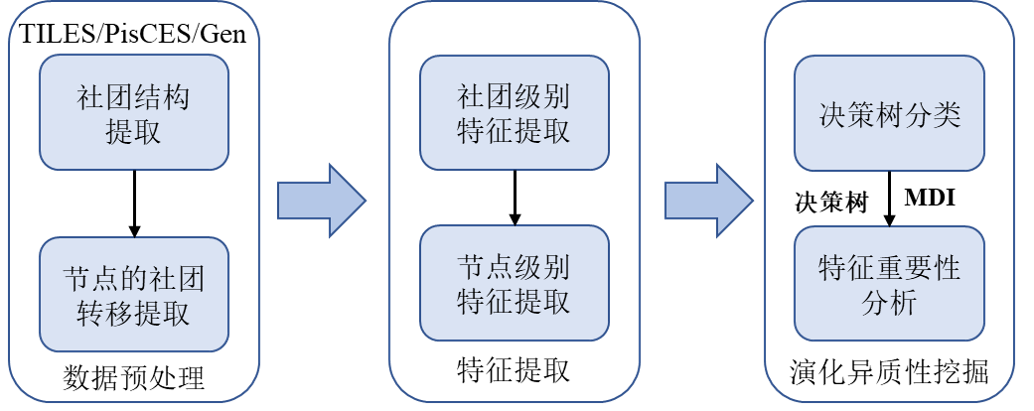
\includegraphics[width=.8\textwidth]{figures/chap03/figure/modelChap3.png}
	\caption{节点社团转移异质性探究方法流程图}
	\label{fig.3.1}
\end{figure}

针对节点社团转移异质性的探究方法如图\ref{fig.3.1}所示,主要分为以下几个步骤:

\begin{enumerate}
\item 动态网络中的社团划分与节点的社团归属变迁分析。本研究首先采用成熟的动态网络社团识别技术,对每一时间快照下的网络社团结构进行解析。为避免单一算法可能引入的偏差,本部分选取三种不同的社团探测方法分别实施,包括GenLouvain算法\cite{GenLouvain}、PisCES方法\cite{PisCes}以及TILES算法\cite{rossetti2017tiles}。为确保动态网络快照划分的一致性,本研究将原始数据格式为$(源节点,目标节点,时间戳)$的动态网络(常见于公开数据集)转化为时间序列形式的网络切片结构,表示为$W={W^1, W^2, \dots, W^T}$,其中$T$代表时间片总数,$W^t \in {0,1}^{N \times N}$则为第$t$时刻的邻接矩阵。通过将相邻快照的节点与社团进行分组,形成多组连续快照网络,并将节点划分为社团不变与社团改变的两组节点,作为后续分类的标签。

\item 节点及社团层面的结构属性提取。本研究基于特征工程的理论基础并参考已有文献的经验性成果\cite{ilhan2016feature},设计并提取了两类共十个结构特征:其一为反映社团整体特性的五个宏观指标,用于探讨社团对节点行为的潜在影响;其二为描述节点个体属性的五个微观指标。具体而言,社团层面特征包括社团规模(节点数量)、社团活跃程度、社团连边数、内部边数、外部边数;节点层面特征则涵盖接近中心性、介数中心性、节点的社团传导性、节点度、邻居平均度。详细定义参见表\ref{fig.3.1}。特征提取的具体流程通过相邻时间片组实现,算法细节见算法\ref{chap3:alg1}。

\item 节点社团变迁的异质性探究。本部分采用决策树模型对节点社团归属变更标签进行分类。在分类完成后,通过计算平均不纯度降低(Mean Decrease in Impurity,MDI)指标,评估各特征在分类任务中的贡献度,从而量化不同结构属性在节点社团变迁过程中的相对重要性。这一分析结果进一步为揭示驱动节点社团归属异质性的深层机制提供了依据。
\end{enumerate}

\begin{algorithm}[!htbp]
	\caption{特征提取}
	\label{chap3:alg1}
	\algorithmicrequire \quad 无向图序列 $W = {W}^1,..{W}^T$ 和社团标签 $\mathcal{C} = \mathcal{C}^1,...\mathcal{C}^T$\\
	\algorithmicensure \quad 分类特征$F$ 和分类标签$L$
	\begin{algorithmic}[1]
		\FOR{图${W}^t$, $t \neq T$}
		\FOR{在$\mathcal{C}^t$的社团 $\mathcal{C}_l^t$  }
		\STATE 统计社团的特征$F_c$
		\FOR{$\mathcal{C}_l^t$中的节点$i$}
		\STATE 计算节点的相关特征$F_n$
		\STATE 组成分类$i$特征序列$F = F_c \vert F_n$
		\IF{$i$的社团标签发生变化}
		\STATE $i$的分类标签$L_i$ = 1
		\ELSE
		\STATE $i$的分类标签$L_i$ = 0
		\ENDIF
		\ENDFOR
		\ENDFOR
		\ENDFOR
	\end{algorithmic}
\end{algorithm}

% \end{enumerate}
在本研究框架的第一阶段,采用了三种已有的社团识别技术,即GenLouvain、PisCES和TILES,以实现动态网络中社团结构的解析。以下为对这三种方法的具体阐述:

\begin{enumerate}
\item GenLouvain是一种基于模块度优化的递归型社团探测算法,其核心目标是通过最大化模块度得分来划分网络社团。该方法通过迭代遍历网络节点对快照网络的社团结构进行识别,并引入了一种创新机制:将同一社团内的节点合并为超节点,从而实现网络结构的粗粒化处理。这种策略使其能够生成多层次的社团划分结果,因而特别适用于处理大规模网络的社团探测任务。

\item PisCES将谱聚类技术扩展至动态网络环境,通过综合分析时间维度信息与网络拓扑特性,追求全局最优的社团划分。该方法首先对所有网络快照的邻接矩阵执行特征分解,提取其特征向量并应用聚类算法(如k-means)进行初步分组。随后,通过引入时间平滑性约束,进一步优化聚类结果,确保社团划分在时间序列上的一致性,从而实现全局优化的社团识别。

\item TILES是一种基于标签传播的社团发现方法,能够识别动态网络中的重叠社团结构,并能够自动划分网络快照,为了保持网络结构一致性,本研究基于TILES所划分的快照进行探究。本研究假设,当某一节点在相邻快照中的社团归属发生显著变化时,可判定该节点经历了社团归属的变迁行为。
\end{enumerate}




在特征提取阶段,本研究探讨了节点与社团两个层级结构在社团演化中的交互影响。研究认为,节点的行为不仅受自身属性驱动,其所属社团的特性同样可能对其行为产生作用,反之亦然。因此,为全面捕捉这种双向关系,本研究也提取了$6$个社团级别的特征来衡量社团对节点演化的影响力。针对节点演化异质性挖掘所构建的节点局部特征如表~\ref{tab.3.1}所示,节点的度、平均邻居度、接近中心性以及介数中心性可以有效衡量节点在网络中的重要程度,而社团级别的特征也可以较全面地衡量社团的特征。

\begin{table}[!htbp]
	
	\centering
	\caption{节点局部特征的定义和符号表示}\label{tab.3.1}
	\vspace{0.5em}\centering\wuhao
	\begin{tabular}{lll}
		% \begin{tabular}{|l|l|l|l|}
			\hline
			符号&节点局部特征名 & 定义\\
			\hline
			$f1$&社团节点数  & $n_l^t$\\
			$f2$&社团边数 & $e_l^t$\\
			$f3$&社团内的边数 & $\frac{e_l^t(in)}{n_l^t}$\\
			$f4$&社团间的边数&  $\frac{e_l^t(out)}{n_l^t}$\\
			$f5$&社团活跃度 & $\frac{a_l^t}{n_l^t}$\\
			$f6$&社团连通率 &  $\frac{e_l^t}{d_l^t}$\\
			$f7$&节点的度 & $e_i^t$ \\
			$f8$&节点的平均邻居度 &  $\frac{1}{|N(i)^t|}\sum_{j\in N(i)^t}e_j^t$ \\
			$f9$&节点的接近中心性 &  $\sum_{j\in C_{l,-i}^t}\frac{C_l^t}{d(i,j)}$ \\
			$f10$&节点的介数中心性 &  $\sum_{j,k \in C_{l,-i}^t}\frac{\sigma_{jk}(i)}{\sigma_{jk}}$\\
			\hline
		\end{tabular}
		
	\end{table}


在特征重要性评估环节,本研究选用决策树作为节点归属变迁的二分类预测工具。相较于深度神经网络等黑箱模型,决策树因其透明性(即白箱特性)而更具优势,能够直观揭示每个特征在分类过程中的贡献。本研究最终采用平均不纯度降低(Mean Decrease in Impurity,MDI)方法\cite{menze2009comparison}量化各特征的重要性。MDI方法能够在决策树中给出各节点对最终分类的影响力大小,且计算效率较高,能够满足本研究的需求。
% ,其计算公式定义如下:

% \begin{equation}
% \centering
% \Delta i(s,r) = i(r) - p_L i(r_L) - p_R i(r_R)
% \end{equation}

% 其中,$i(r)$表示某一不纯度指标(如基尼指数),$r$为决策树中的某个分裂节点,$r_L$和$r_R$分别代表其左、右子节点。比例系数$p_L = N_{r_L}/N_r$表示左子节点的数据量占父节点数据量$N_r$的比例,类似地,$p_R = N_{r_R}/N_r$。通过标准化处理后的$\Delta i(s,r)$,可为每个特征生成一个重要性得分。此方法计算效率高,适用于大规模数据集的分析需求。









\subsection{规律挖掘数据描述}

% 本章所用数据集包括Internet、Facebook、Digg、Wikipedia等共$15$个不同类型的公开动态网络数据集以尽可能覆盖大部分常见的网络类型,对于数据集的详细描述见表\ref{tab.3.2}。如图\ref{fig.3.2}所示,用于研究的所有数据集均符合重尾分布,且同一来源的不同主题数据之间的度分布也存在偏差,这一定意义上证了本研究对真实世界数据挖掘任务的覆盖面。

本章研究所采用的数据集涵盖了Internet、Facebook、Digg、Wikipedia等在内的共15个公开动态网络数据集,旨在尽可能囊括多种常见的网络类型。有关各数据集的具体信息,可参见表\ref{tab.3.2}中的详细说明。


\begin{table}[!htbp]
	\centering
	\caption{数据集及其描述}\label{tab.3.2}
        \vspace{0.5em}\centering\wuhao
	\resizebox{\textwidth}{!}{
		\begin{tabular}{p{70pt}p{250pt}p{55pt}p{40pt}}
			\hline
			数据集&数据内容 & 节点数$|\mathcal{V}|$ & 边数$|\mathcal{E}|$\\
			\hline
			ia-digg-reply &Digg社交网站网络\cite{nr},时间跨度为2008年10月29日至2008年11月13日 & $30397$ & $87627$\\
			ia-facebook-wall-wosn-dir & Facebook关注与被关注网络\cite{nr},时间跨度2004年5月15日至2004年10月24日 & $44668$ & $876993$\\
			ia-reality-call & MIT的手机接打电话网络\cite{nr},时间跨度为 2004年9月24日-2005年10月7日& $6810$ & $52050$\\
			ia-slashdot-reply-dir & Slashdot\cite{nr}网站的问答网络,时间跨度为2005年12月7日-2006年8月31日 & $51097$ & $140778$\\
			ia-stackexch-user-marks-post & StackOverflow\cite{nr}的问答网络,时间跨度为2008年10月3日-2011年11月25日 & $545196$ & $1302439$\\
			ia-yahoo-messages & 雅虎\cite{nr}的消息网络,时间跨度未知& $99303$& $3179718$\\
			soc-epinions-trust-dir & Epinion的关联网络\cite{nr},时间跨度未知& $131828$ & $841373$\\
			soc-wiki-elec & Wikipedia的页面投票网络\cite{nr},时间跨度2004年9月14日-2008年1月5日 & $8271$ & $107071$\\
			wiki& Wikipedia网页关联网络\cite{mislove-2009-socialnetworksthesis},时间跨度2001年2月20日-2002年12月6日 & $329623$ &$39953145$\\
			Internet & 因特网\cite{mislove-2009-socialnetworksthesis}数据,时间跨度2004年1月4日 -2005年4月4日& $33936$ & $104824$\\
			Facebook & 脸书在新奥尔良地区的交友网络\cite{viswanath-2009-activity} ,时间跨度 2008年8月6日-2009年1月21日&$62306$& $905565$\\
			bitcoin & 比特币\cite{kumar2016edge}的信任链网络,时间跨度2010年11月9日-2016年1月19日 & $5881$ & $35592$\\
			Friend & 美国某社区的现实世界交友网络\cite{aharony2011social},时间跨度2010年7月10日-2011年7月16日 & $130$ & $60518$\\
			fb-forum & 脸书某论坛帖子网络\cite{nr},时间跨度2004年5月15日-2004年10月24日 & $899$ & $33720$\\
			fb-messages & 脸书加州学生社区的消息网络\cite{nr},时间跨度2004年3月 24日-2004年10月22日 & $1897$ & $61734$\\

			\hline
		\end{tabular}
	}
\end{table}


% \begin{figure}[!htbp]
% 	\setlength{\abovecaptionskip}{0pt} 
% 	\setlength{\belowcaptionskip}{10pt} 
% 	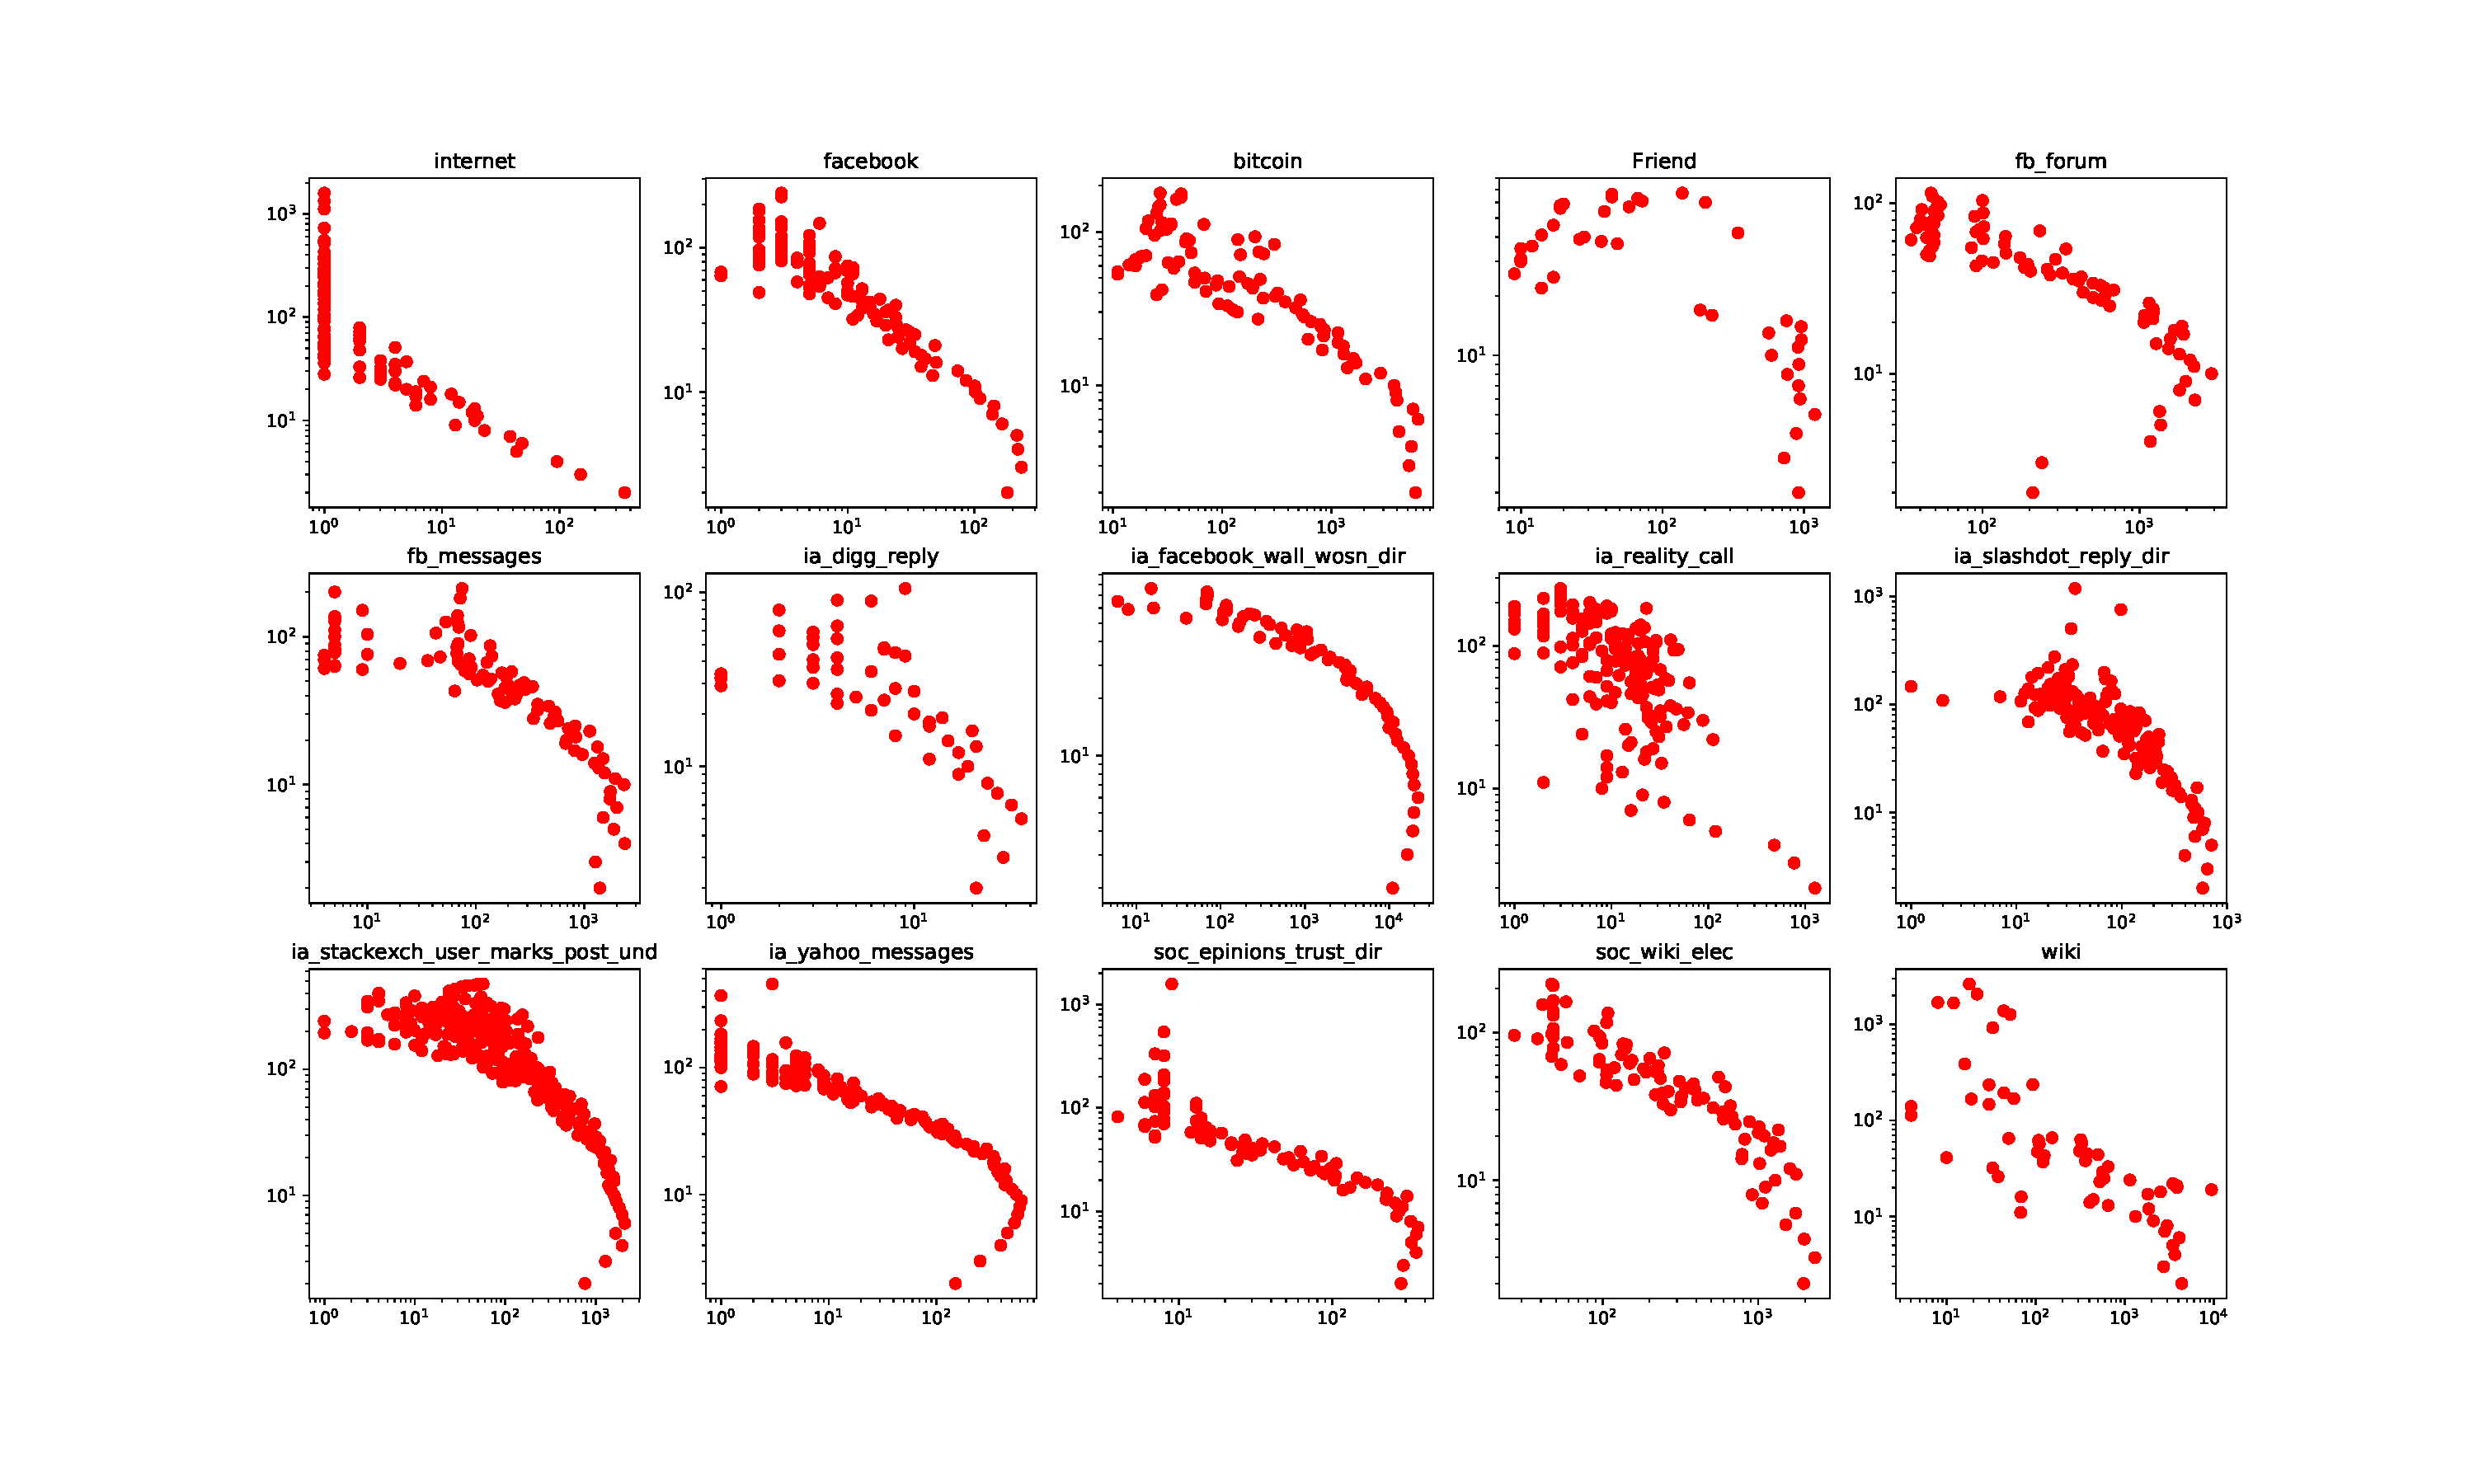
\includegraphics[width=.9\textwidth]{figures/chap03/figure/degrees.pdf}
% 	\caption{15个真实数据集的度分布可视化}
% 	\label{fig.3.2}
% \end{figure}

\subsection{挖掘结果}

% \subsubsection{实验及结论}

% 按照上文所述的研究框架处理上述$15$个数据集,并计算其特征重要性。结果如图\ref{fig.3.3}所示,图中横坐标表示节点如表\ref{fig.3.1}所述的分类特征;纵坐标分别表示$15$个数据集,颜色代表特征在不同数据集中的分类任务中所占重要性,颜色越浅表示该特征重要性越高。可以看到$f7$(节点的度)与$f8$(节点的平均邻居度)在所有特征分类中均占很大比重,尤其在$fb-forum$数据中,节点的平均邻居度在分类中所占比重超过了$0.5$;而$f5$(社团活跃度)在$ia-slashdot-reply-dir$数据中所占比重超过其他数据,该数据为技术网站Slashdot的回复网络,从这一点来看,\textbf{科技类网站的圈子活跃度}是影响其用户更换兴趣圈的主要因素;与此同时,在$internet$网络中,$f9$(节点的接近中心性)对其节点的社团转移影响最大,显而易见,在因特网中,连通性是其最至关重要的指标之一。虽然$f5,f9$均在某些数据集中显示出了对节点社团转移的重要影响力,但是其并不具有普遍性。反观$f7,f8$,其在所有数据集中对节点的社团转移均具有可观的影响力。因此本研究可得出初步结论,\textbf{节点的度以及节点的平均邻居度是影响节点发生社团转移的重要的结构特征}。进一步可以确定,节点的社团转移存在异质性,即\textbf{社团内不同的节点具有不同的转移倾向性}。

% 另外,为了去除社团检测算法偏差,本研究基于GenLouvain和PisCES两个社团检测算法的结果如图~\ref{fig.3.3Gen}和图~\ref{fig.3.3Pis}所示,其结果也证实了本研究的结论,即社团内不同节点具有不同的转移倾向,但细节方面存在一定偏差,如节点级特征$f9,f10$在GenLouvain方法中具有更大的占比,而在PisCES中$f7$节点的度在$ia_reality_call$数据集中相较于另外两个社团检测方法具有更高的重要性。
通过对上述数据集的挖掘,结果如图~\ref{fig.3.3}所示。热图中横坐标代表特征编号,纵坐标代表数据集,颜色越浅表示分类特征重要性越高。可以看到,去除社团检测算法差异后,节点级别的特征在社团转移过程中占有较高的重要性,其中以节点的平均邻居度和节点的度对分类影响最大,即\textbf{动态网络中,社团内不同的节点具有不同的社团转移倾向性,且单独的某一个特征并不能决定节点的社团转移}。这也证明了在动态网络生成过程中,节点的高阶特征如平均邻居度对网络及社团演化具有显著的影响,这为后续模型对动态网络生成模式的建模提供了实证依据。


\begin{figure}[!htbp]
        \subfigure[基于TILES]{
        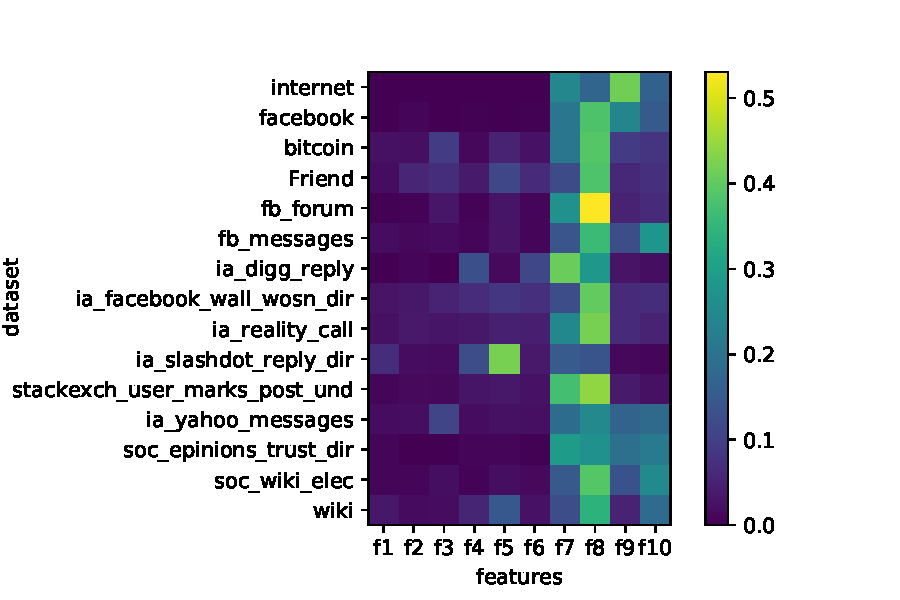
\includegraphics[width=.31\textwidth]{figures/chap03/figure/15cmp.pdf}
        }
	\subfigure[基于GenLouvain]{
    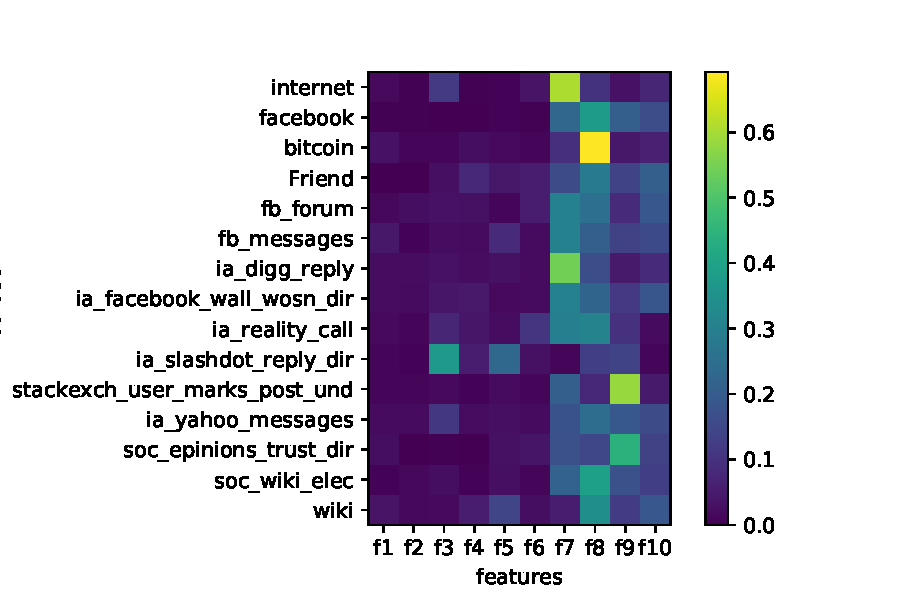
\includegraphics[width=.31\textwidth]{figures/chap03/figure/resultGenlou.pdf}
        }
        \subfigure[基于PisCES]{
    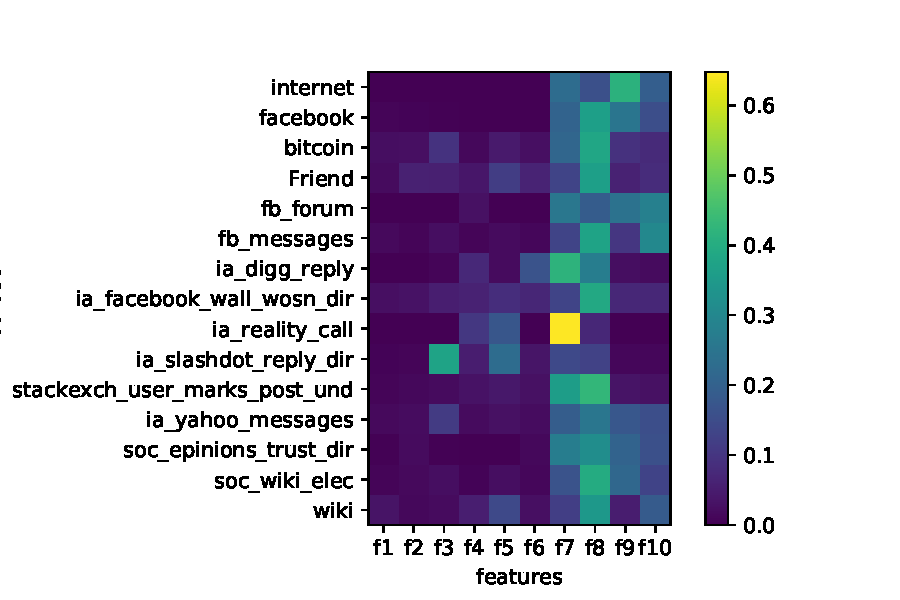
\includegraphics[width=.31\textwidth]{figures/chap03/figure/resultPNAS15.pdf}
        }
	\caption{基于不同社团检测算法的$15$个数据集的特征重要性热图}
	\label{fig.3.3}
\end{figure}
% \begin{figure}[!htbp]
% 	\setlength{\abovecaptionskip}{0pt} 
% 	\setlength{\belowcaptionskip}{10pt} 
% 	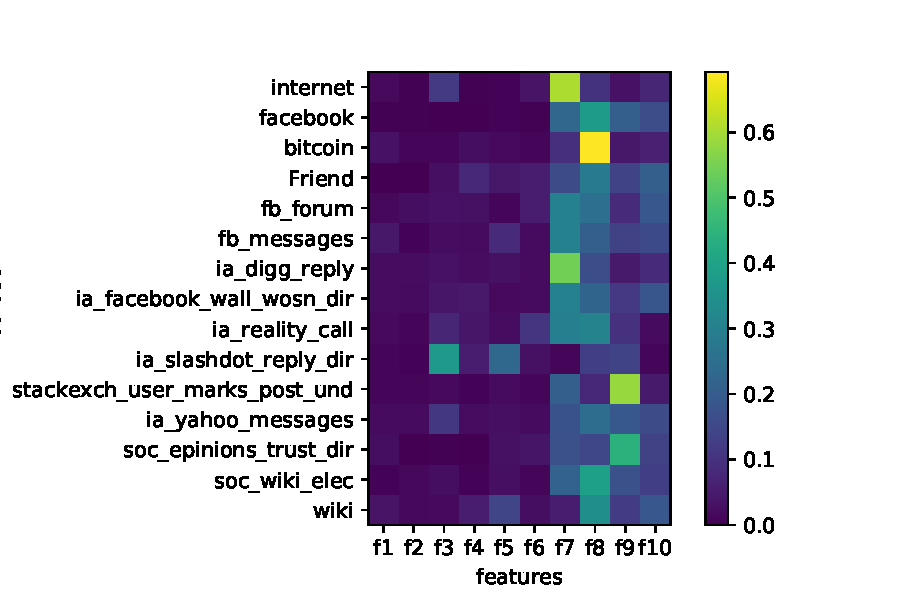
\includegraphics[width=.9\textwidth]{figures/chap03/figure/resultGenlou.pdf}
% 	\caption{基于GenLouvain的$15$个数据集的特征重要性热图}
% 	\label{fig.3.3Gen}
% \end{figure}
% \begin{figure}[!htbp]
% 	\setlength{\abovecaptionskip}{0pt} 
% 	\setlength{\belowcaptionskip}{10pt} 
% 	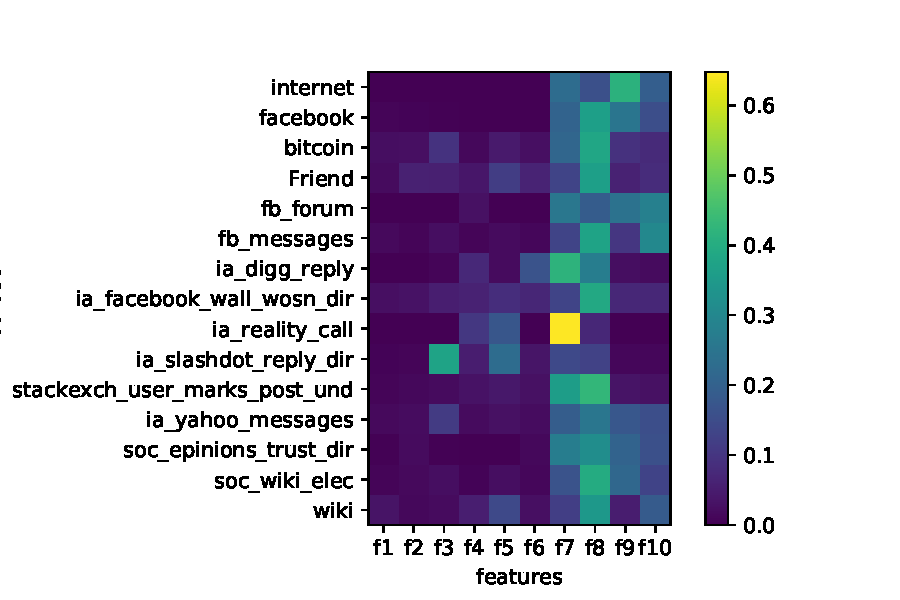
\includegraphics[width=.9\textwidth]{figures/chap03/figure/resultPNAS15.pdf}
% 	\caption{基于PisCES的$15$个数据集的特征重要性热图}
% 	\label{fig.3.3Pis}
% \end{figure}

% 为了探究节点的度以及节点的平均邻居度是以何种模式影响节点的社团转移的,本文分别统计了以上两个节点结构属性在$15$个数据集中的分布。如图\ref{fig.3.4}所示,该图展示了节点的度在十五个数据集中的分位图,每个子图中共有两列分位图,分别为发生转移的节点(横坐标为$1$)以及未发生转移的节点(横坐标为$0$)的度的分位统计图。从图中可以看到,在所有$15$个数据集中,发生社团转移的节点的度普遍比未发生转移的节点的度更高,即在一个网络中,节点的度越高,其越有可能发生社团转移。这也验证了社团检测中的大量度修正方法~\cite{wilson2016modeling,jin2015modeling}的正确性。而图\ref{fig.3.5}则展示了节点的平均邻居度在十五个数据集中的分位图,每个子图中共有两列分位图,分别为发生转移的节点(横坐标为$1$)以及未发生转移的节点(横坐标为$0$)的平均邻居度的分位统计图。可以看到节点的平均邻居度在不同数据集中的发生转移以及未发生转移节点中的值并不相同,这说明不同的节点平均邻居度确实在影响节点的社团转移行为,然而其模式在所有十五个数据集中并不统一。

% \begin{figure}[!htbp]
% 	\setlength{\abovecaptionskip}{0pt} 
% 	\setlength{\belowcaptionskip}{10pt} 
% 	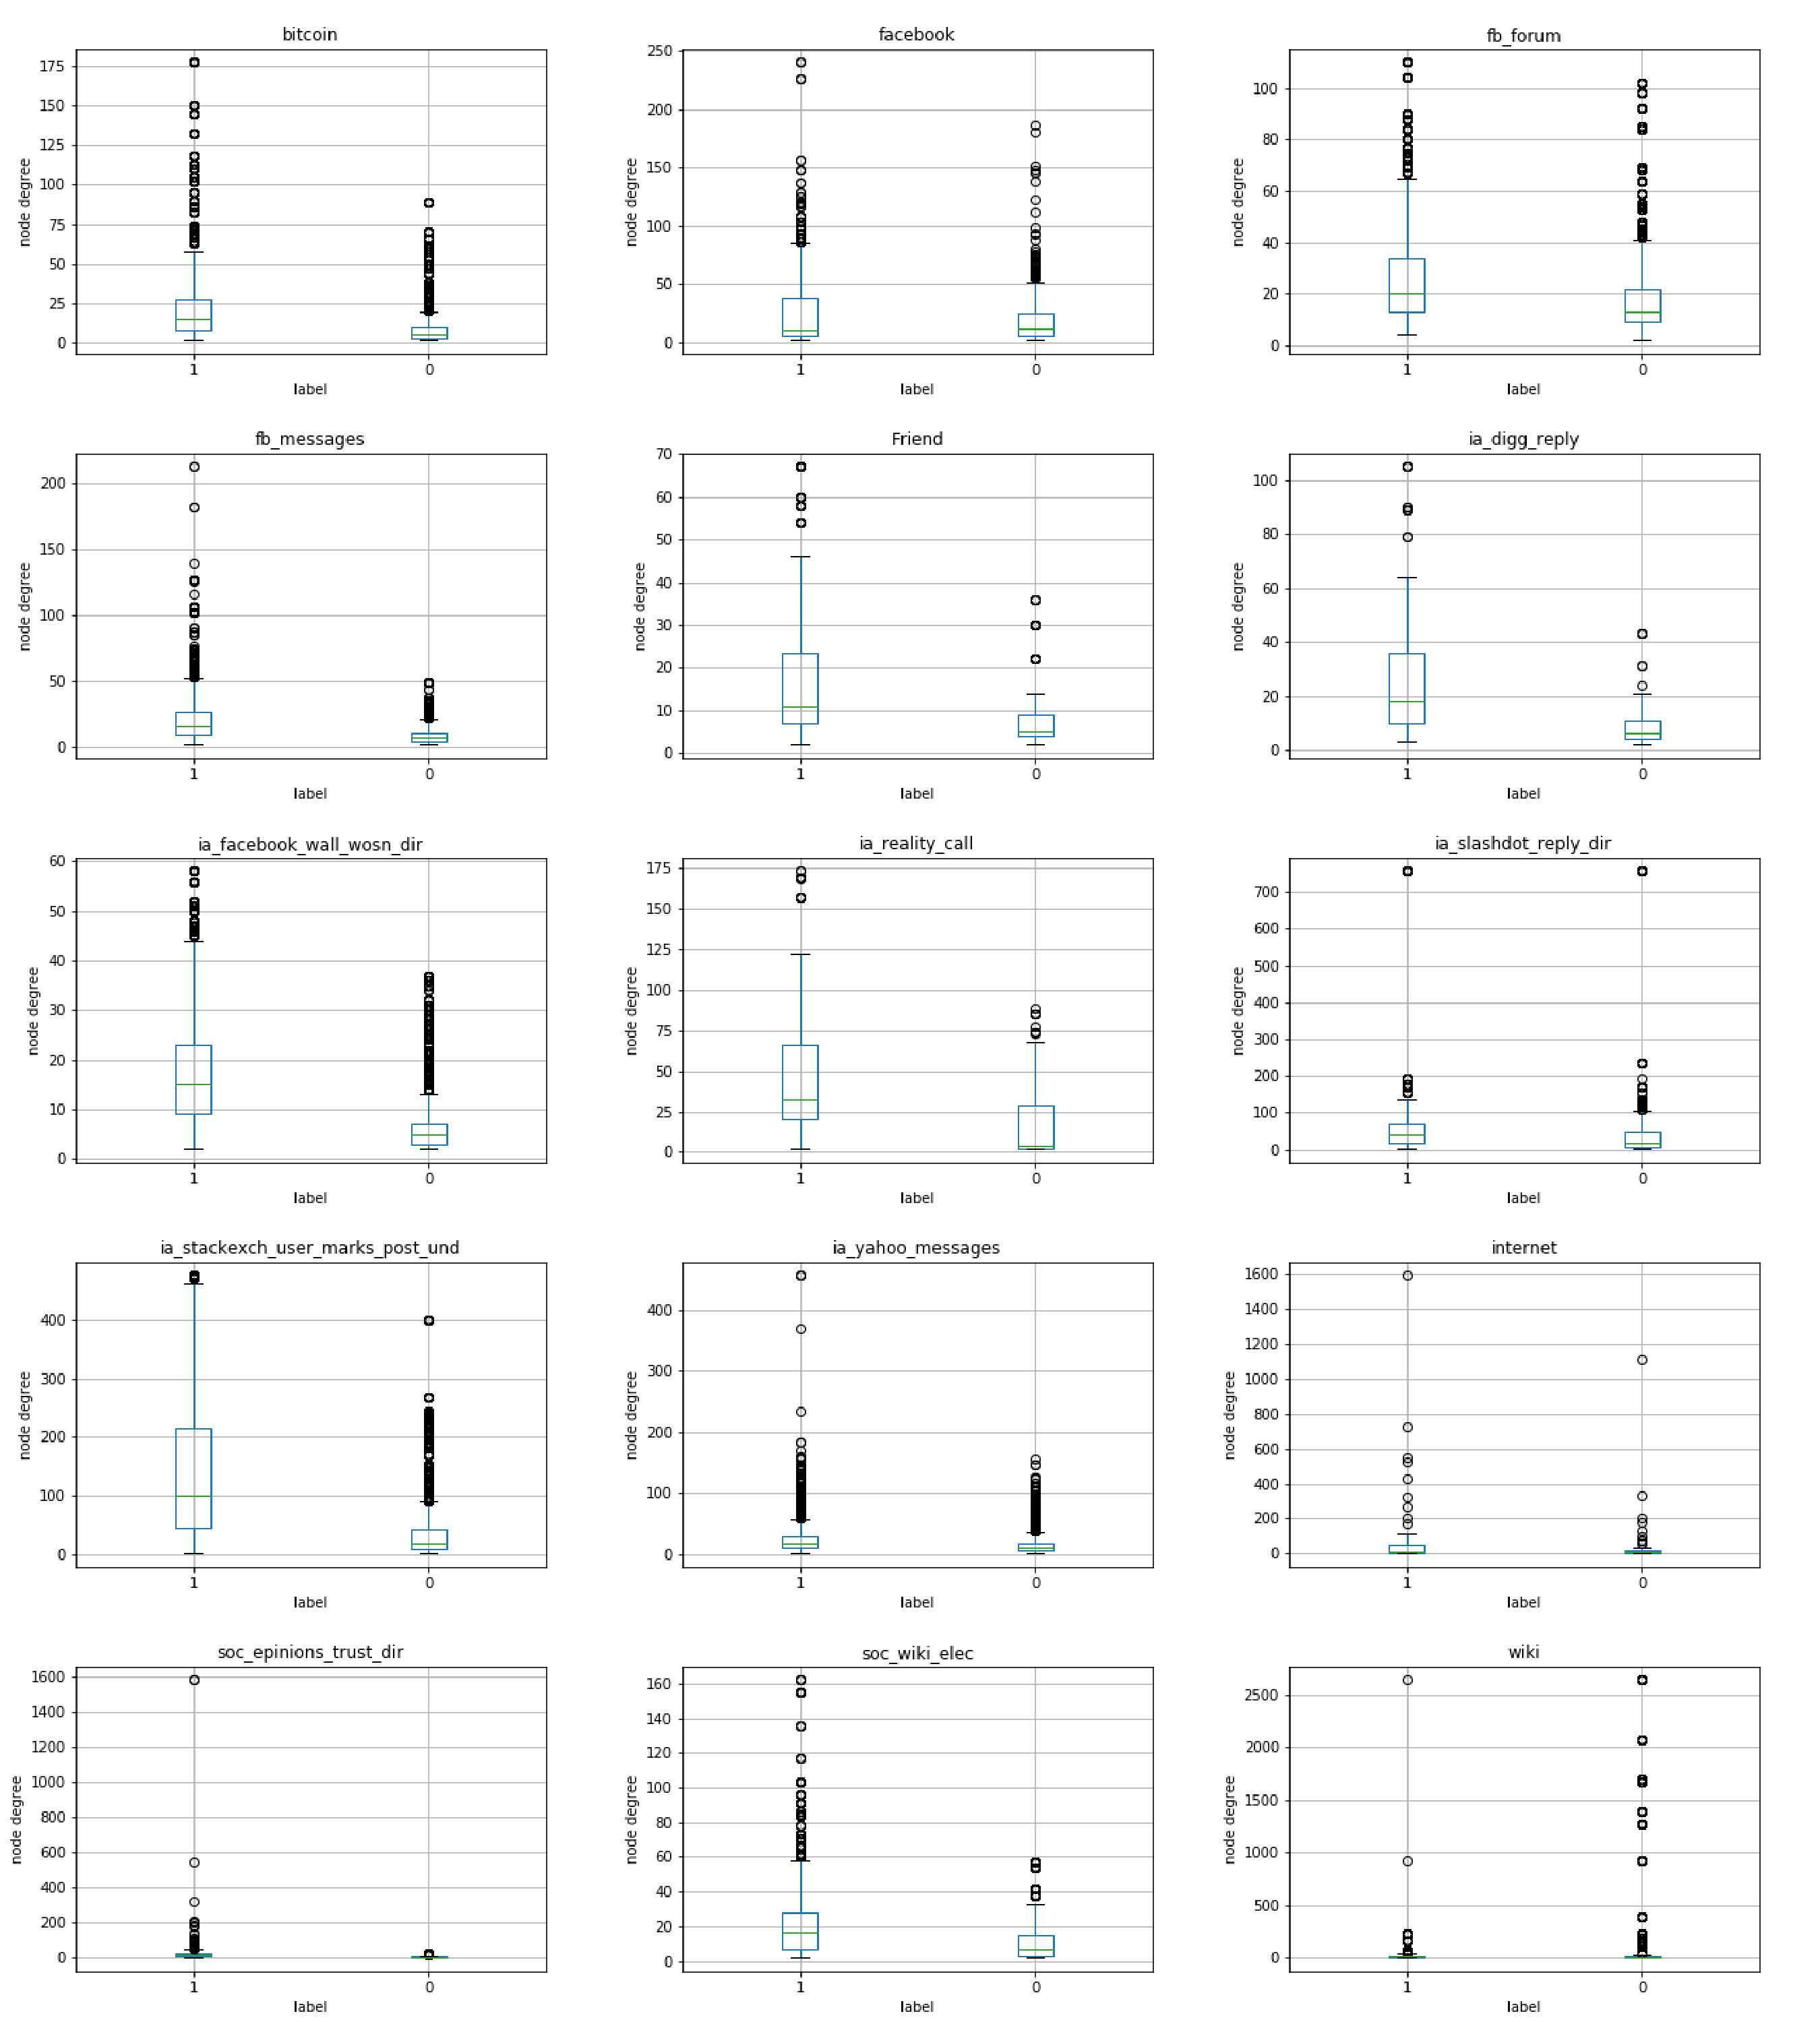
\includegraphics[width=.9\textwidth]{figures/chap03/figure/alldata-DG.pdf}
% 	\caption{15个数据集的节点度的分位图}
% 	\label{fig.3.4}
% \end{figure}

% \begin{figure}[!htbp]
% 	\setlength{\abovecaptionskip}{0pt} 
% 	\setlength{\belowcaptionskip}{10pt} 
% 	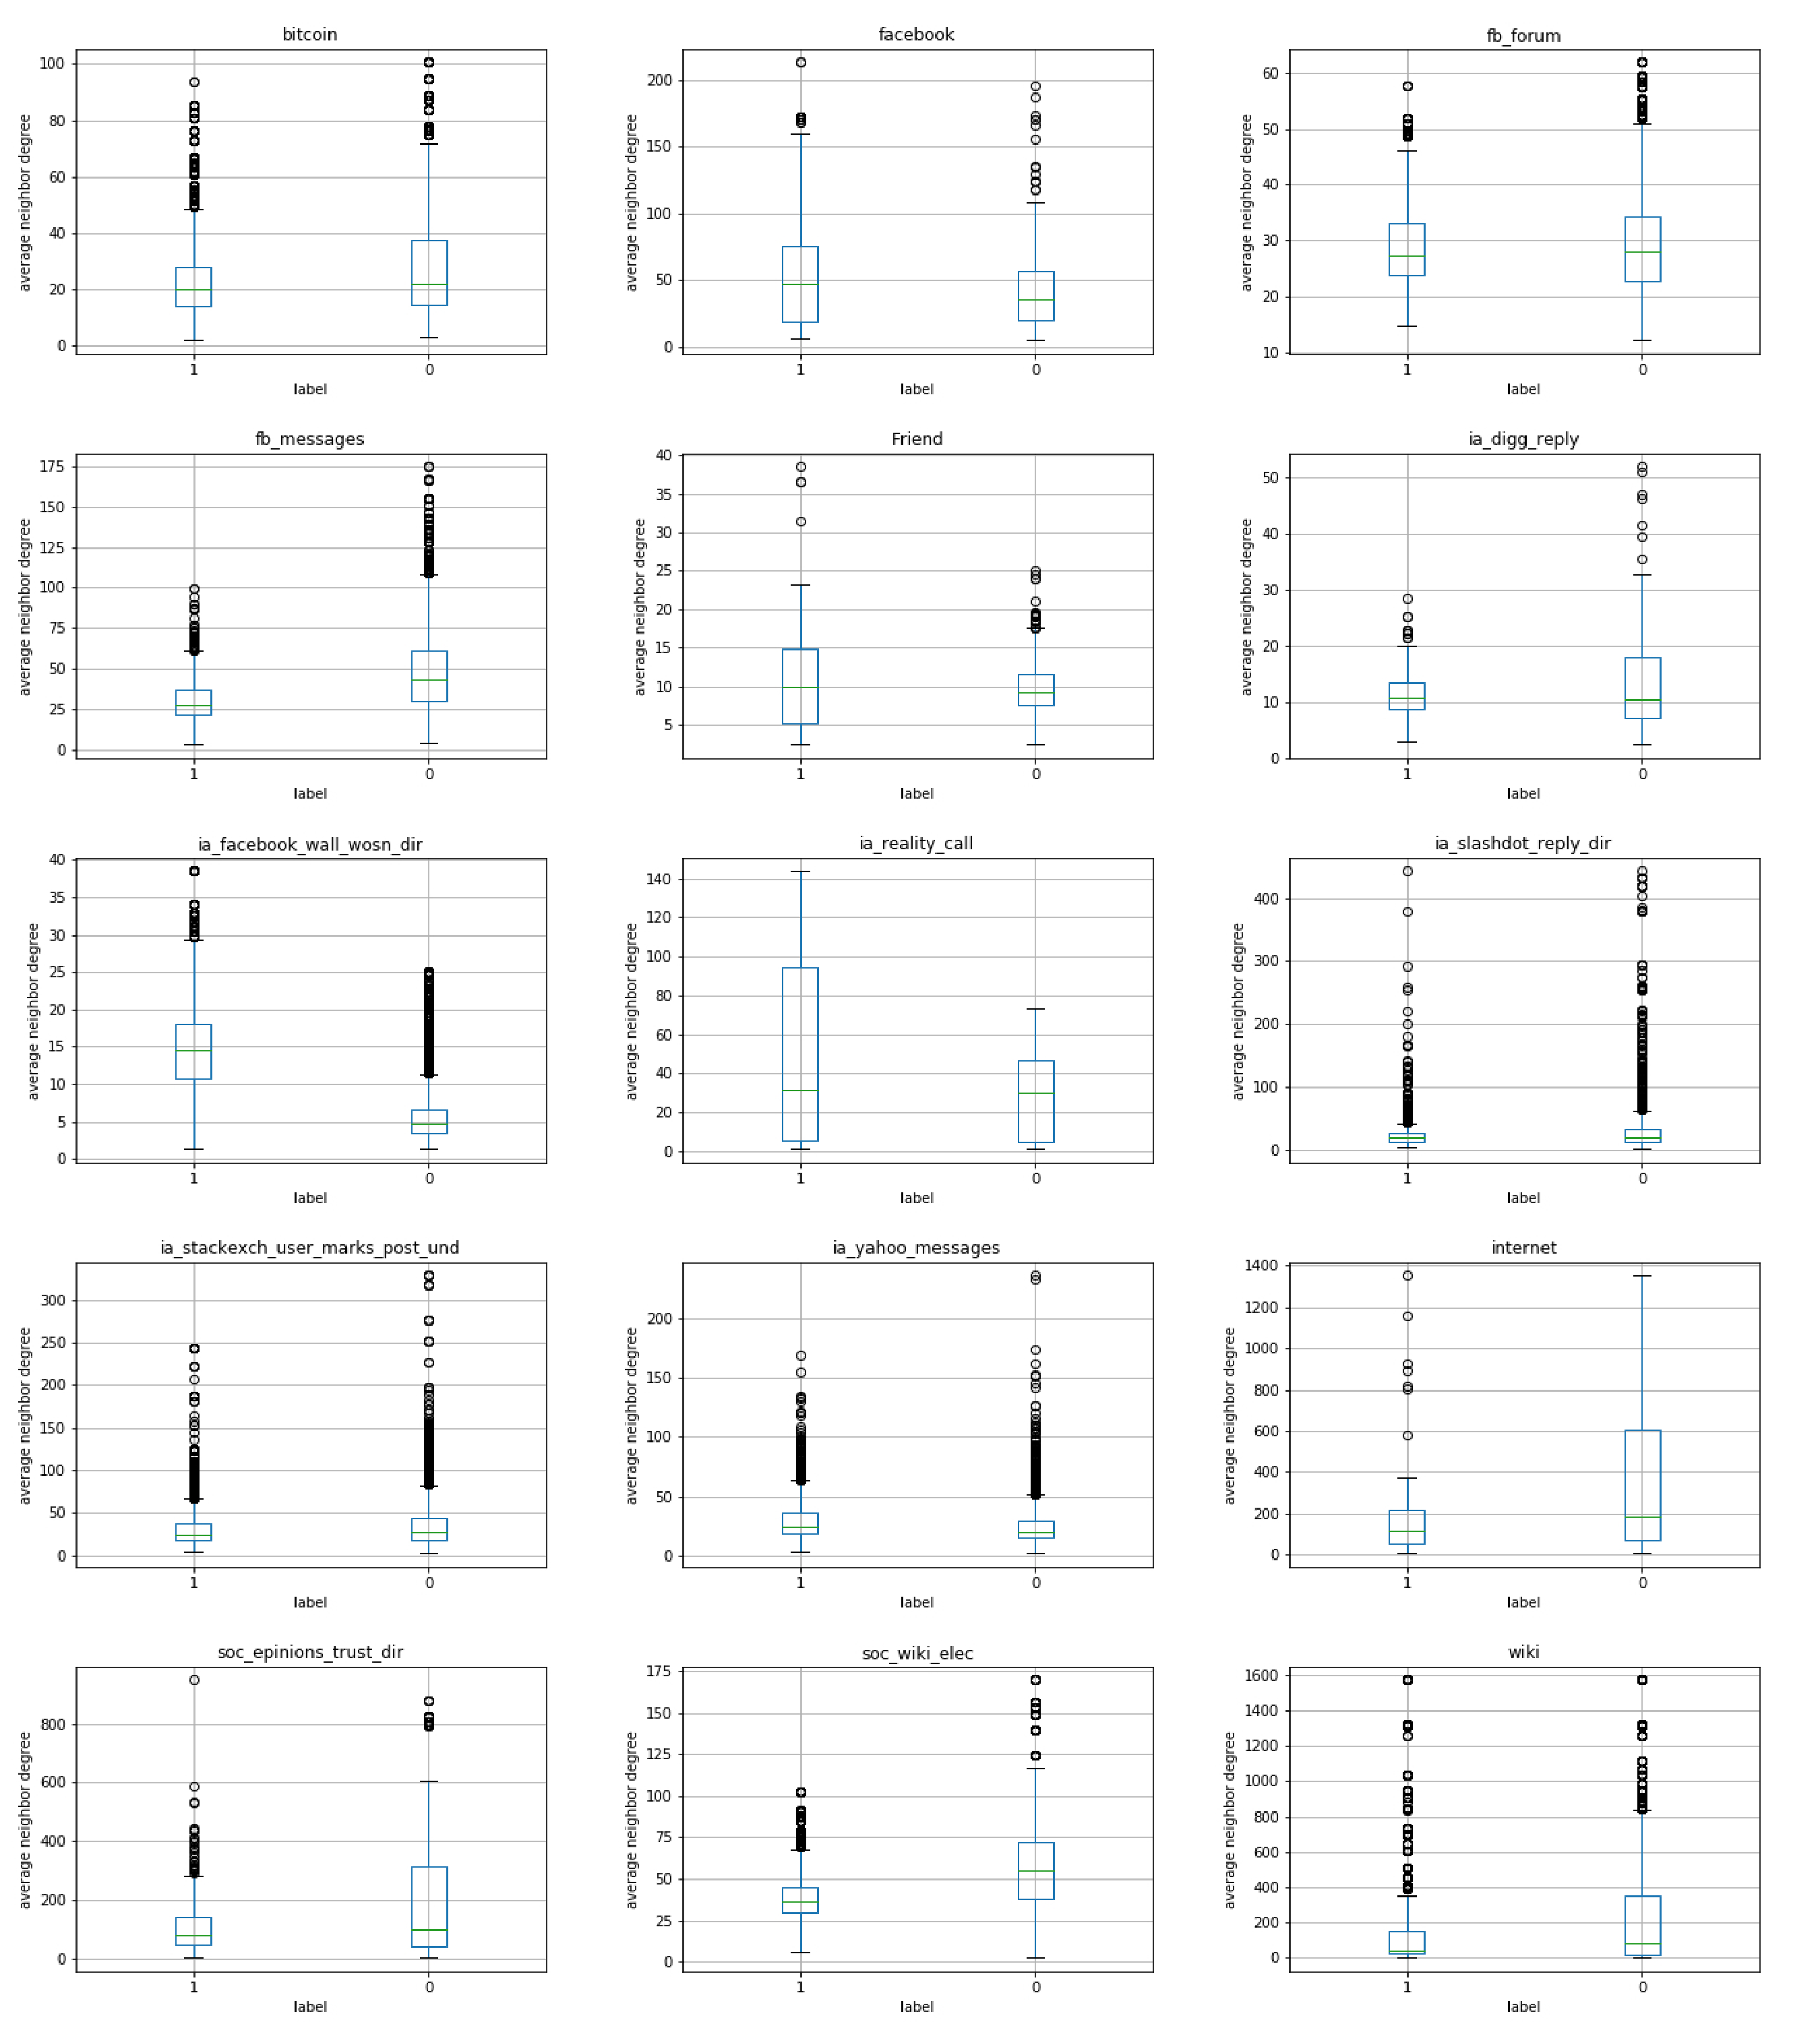
\includegraphics[width=.9\textwidth]{figures/chap03/figure/alldata-aND.pdf}
% 	\caption{15个数据集的节点的平均邻居度的分位图}
% 	\label{fig.3.5}
% \end{figure}



\section{融合节点社团转移异质性的动态随机块模型}
上述研究从实际数据集的角度证明了节点在动态网络中社团转移异质性的存在,受此启发,本文提出了基于动态随机块模型DSBM的层次贝叶斯动态随机块模型HB-DSBM。

\subsection{符号表示}


% 在介绍模型前,本节首先介绍模型的符号表示。如表\ref{tab.4.1}所示,用$W=\{W^1,W^2,...,W^T\}$表示动态网络邻接矩阵,即$W^t$表示第$t$个网络快照的邻接矩阵,其中$t \in 1,...,T$。这里$W^t \in \{0,1\}^{N\times N}$,$W_{ij}^t = 0$则代表$i$节点与$j$节点在网络快照$t$中没有边,若为$1$则有边。这里为了方便叙述,本章认为网络是无向无权的,这里需要说明,HB-DSBM可以有效的扩展为有向有权网络。$Z = \{Z^1,Z^2,...,Z^T\}$代表每个网络快照中节点的社团划分,例如$z_i^t = k$则表示$i$节点在网络快照$t$中属于$k$社团,其中$k\in K$。

在正式介绍模型之前,本节首先阐释本章的符号体系。如附录A.1~表\ref{symbols:all}所示,动态网络的邻接矩阵集合用$W={W^1, W^2, \dots, W^T}$表示,其中$W^t$对应第$t$个网络快照的邻接矩阵,$t$取值范围为$1$至$T$。本章中,$W^t \in {0,1}^{N \times N}$,$W_{ij}^t = 0$表示在快照$t$中节点$i$与节点$j$之间不存在边,而$W_{ij}^t = 1$反之。为了方便描述,本章假设输入的网络是无向且无权的。对于无向无权网络,可以通过设置邻接矩阵非对称或邻接矩阵的数值为大于等于$0$的整数,并将连边分布设置为泊松分布进行适配。$Z = {Z^1, Z^2, \dots, Z^T}$则表示动态网络每个快照的社团划分,当$z_i^t = k$时,表示节点$i$在$t$时刻属于社团$k$,$k \in K$,$z_i$也可以用one-hot向量进行表示。

\subsection{HB-DSBM模型设计}

\begin{figure}[!htbp]
	\setlength{\abovecaptionskip}{0pt} 
	\setlength{\belowcaptionskip}{10pt} 
	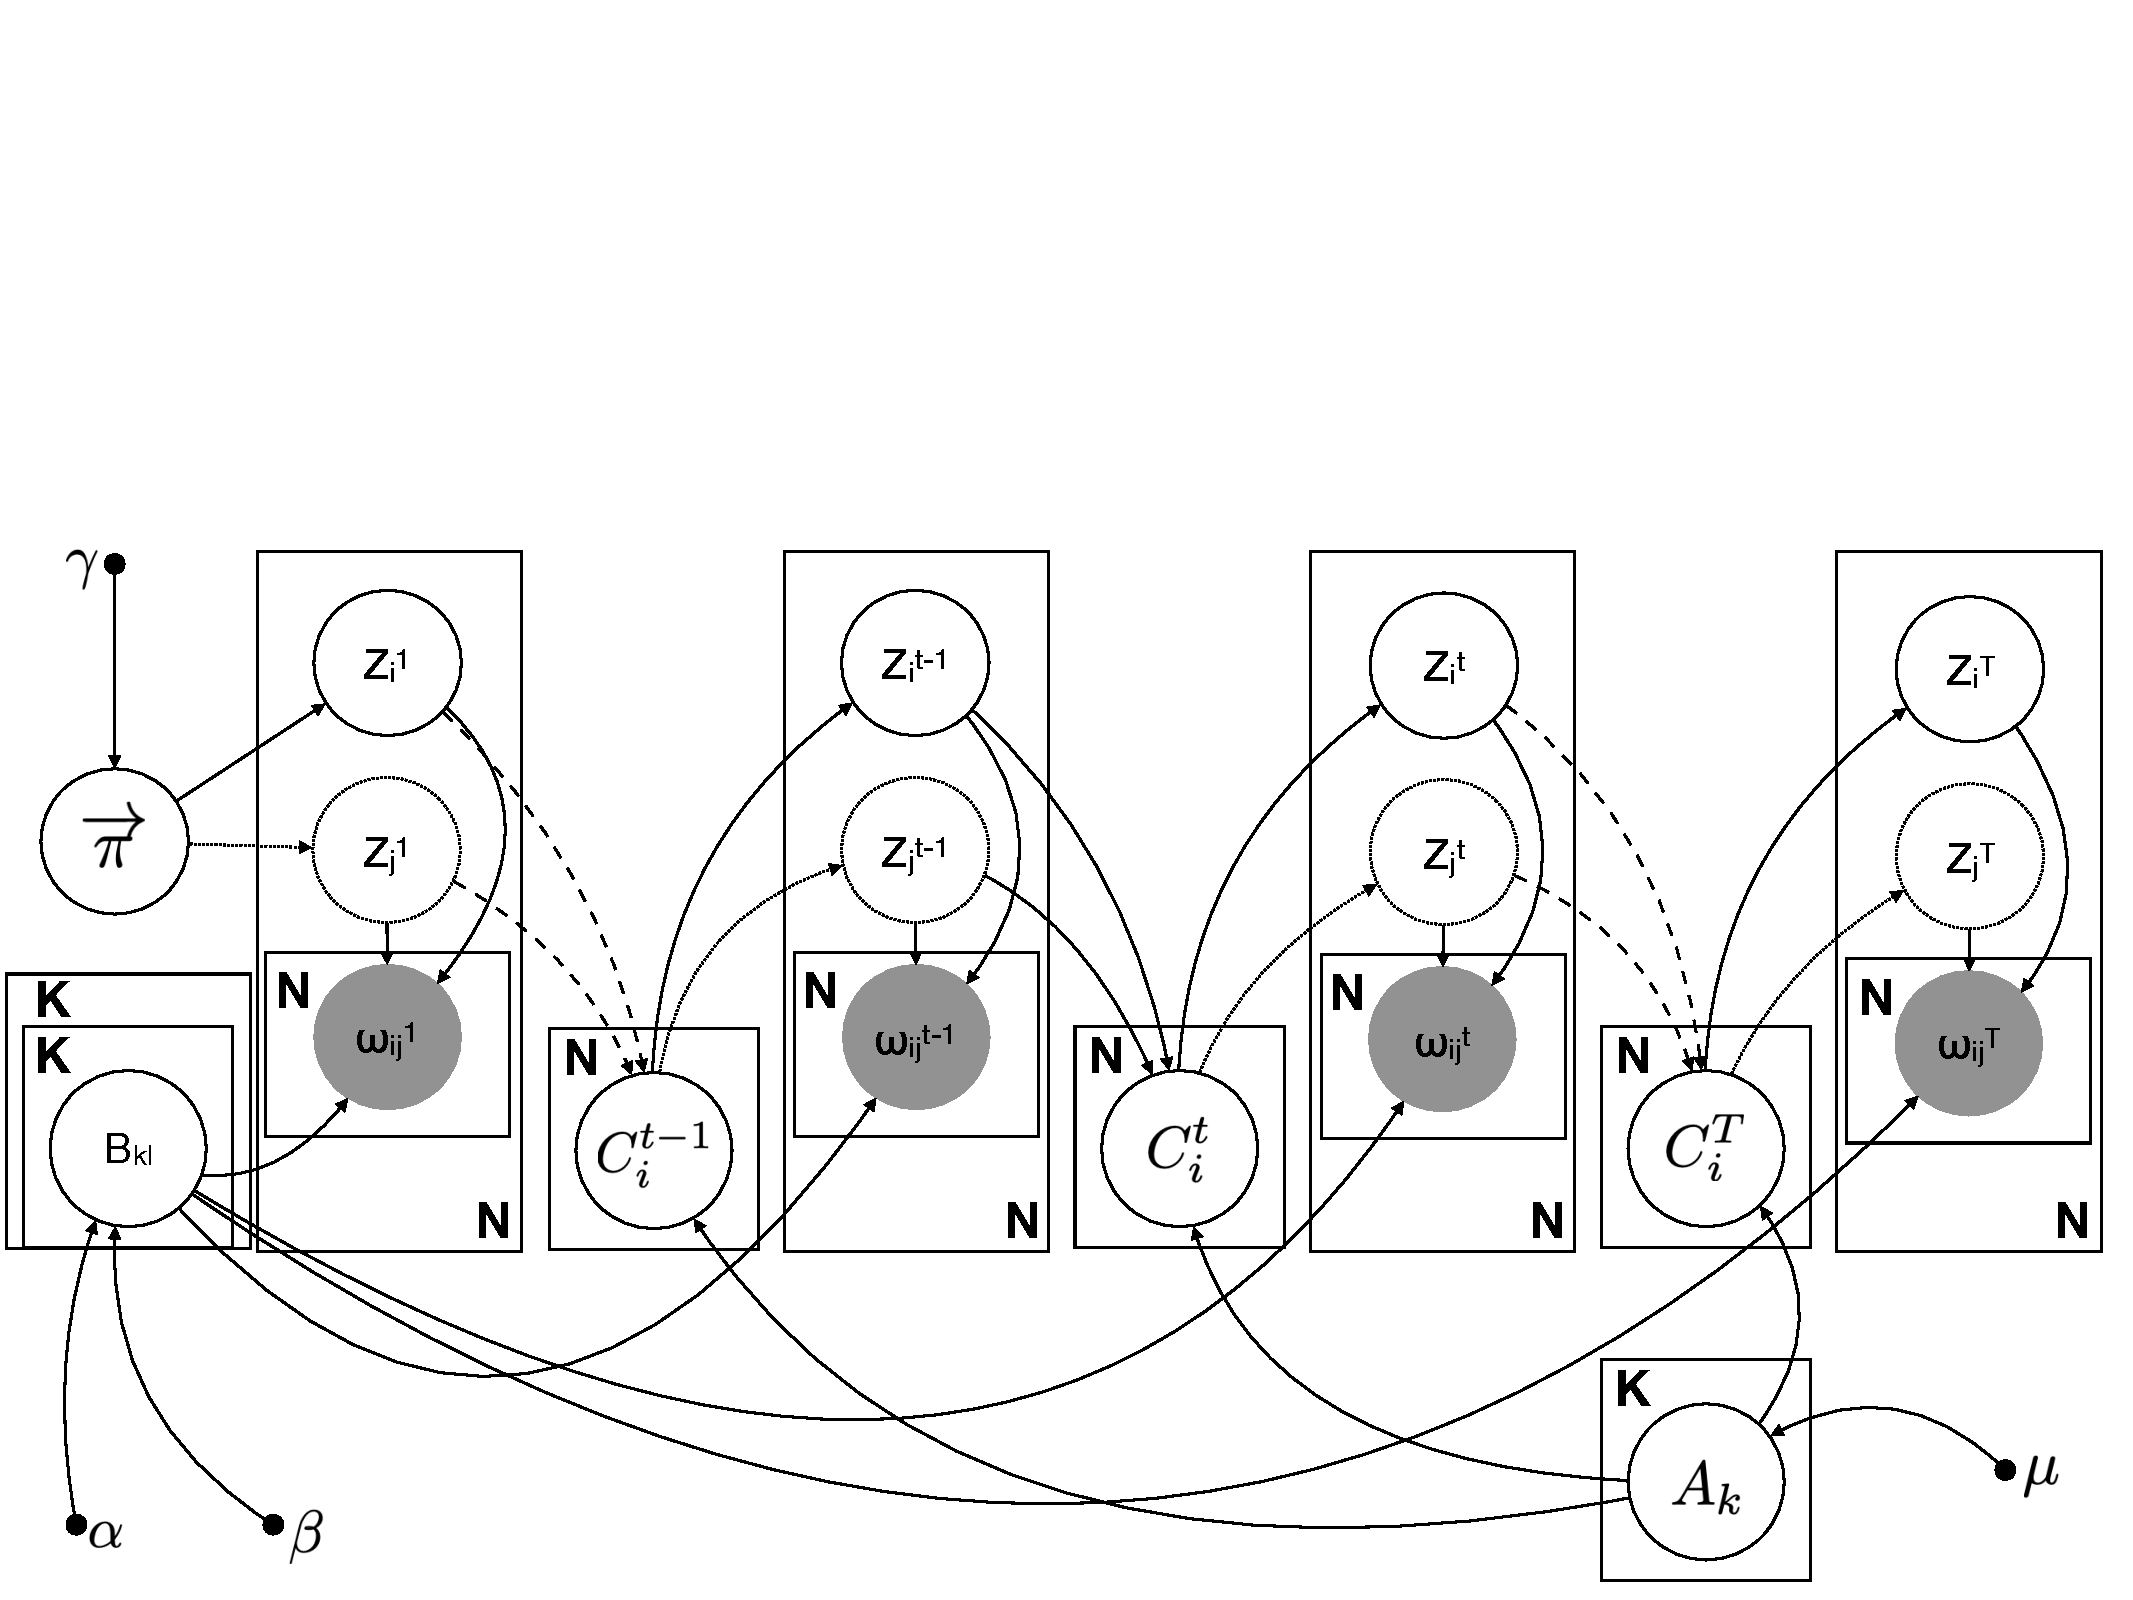
\includegraphics[width=.9\textwidth]{figures/chap04/graph-model_v3_cuted.pdf}
	\caption{HB-DSBM图模型}
	\label{fig.4.1}
\end{figure}

% 本节首先介绍HB-DSBM的核心生成机制来揭示它是如何通过层次贝叶斯结构同时建模社团级别和节点级别的动态演化的,随后给出其产生社团结构和动态网络的生成过程。

% 如图~\ref{fig.4.1}的图模型所示,HB-DSBM首先令$\pi$表示$Z^1$的先验分布,同时$\pi$服从参数为$\gamma$的狄利克雷分布。$B$是不同社团间节点的连边概率,即类随机块模型中的块矩阵,例如$B_{kl}$即代表属于$k$社团和属于$l$社团的节点之间连边的伯努利分布概率。而$B$服从参数为$\alpha$和$\beta$的Beta分布。

% 本章中的$A \in [0, 1]^{K \times K}$表示社团级别转移倾向矩阵,$A$的每一行$A_k$都服从参数为$\mu$的狄利克雷分布,因此 $\sum_l A_{kl} = 1$。同时$C = \{ C^2, \cdots C^T \}$表示节点级别的社团转移倾向,每个$C^t$都是由社团级别转移倾向矩阵$A$生成。对于$t>1$的网络快照,任意节点$i$都有其唯一的转移向量 $C_i^t  \in [0, 1]^K$,该向量服从以参数为$A_{z_i^{t-1}}$的狄利克雷分布,因此$\sum_{k} C_{ik}^t = 1$。这一部分就是本模型的核心:层次狄利克雷生成机制。

% 基于以上机制,模型可以生成社团标签以及动态网络中每个网络快照中的边。具体生成过程如下所示:
% \begin{enumerate}
% 	\item 生成初始社团划分概率 ${\pi} \sim Dir({\gamma})$
% 	\item 生成块矩阵 $B \sim Beta({\alpha},{\beta})$
% 	\item 对于网络快照$t=1$的每个节点$i$:
% 	\begin{enumerate}
% 		\item 生成每个节点的社团归属 $z_i^1 \sim Mult({\pi})$ 
% 		\item 生成每条边 $\omega_{ij}^1 \sim Bernoulli(\cdot | B_{z_i^1,z_j^1})$
% 	\end{enumerate}
% 	\item 生成每个社团级别转移矩阵的社团转移向量 ${A}_k \sim Dir({\mu})$
% 	\item 对网络快照$t>1$中的每个节点$i$:
% 	\begin{enumerate}
% 		\item 生成每个节点级别的社团转移向量${C}_i^t \sim Dir({A}_{z_i^{t-1}})$
% 		\item 生成每个节点的社团归属 $z_i^t \sim Mult({C}_i^t)$
% 		\item 生成每条边 $\omega_{ij}^t \sim Bernoulli(\cdot | B_{z_i^t,z_j^t})$
% 	\end{enumerate}
% \end{enumerate}



首先介绍本方法的生成机制,详细介绍所设计的层次狄利克雷生成结构如何生成节点级别的社团转移倾向矩阵,然后介绍整个网络的生成过程。


如图~\ref{fig.4.1}所示,首先$Z^1$的先验分布为以$\pi$为参数的分类分布,而$\pi$则服从以$\gamma$参数的Dirchlet分布。$B$表示动态随机块中的连边概率,即块矩阵,其服从以$\alpha$和$\beta$为参数的Beta分布。

$A \in [0, 1]^{K \times K}$表示社团级别的转移倾向矩阵,$A_k$服从以$\mu$为参数的Dirchlet分布,并满足$\sum_l A_{kl} = 1$。$C = { C^2, \dots, C^T }$则表示节点的社团转移倾向,$C^t$由$A$进行生成。当$t>1$时,节点$i$的社团转移倾向为$C_i^t \in [0, 1]^K$,服从以$A_{z_i^{t-1}}$为参数的Dirchlet分布,且$\sum_{k} C_{ik}^t = 1$。这一层次生成机制由Dirchlet分布构成,因此本文称之为层次狄利克雷生成结构,也是本模型对节点的演化异质性建模的核心。

综上所述,HB-DSBM的生成过程如下:
\begin{enumerate}
\item  生成$t=1$时的社团划分先验分布${\pi} \sim Dir({\gamma})$;
\item 生成块矩阵$B \sim Beta({\alpha}, {\beta})$;
\item 对$t=1$的节点$i$:
\begin{enumerate}
\item 生成初始社团划分$z_i^1 \sim Mult({\pi})$;
\item 生成边 $\omega_{ij}^1 \sim Bernoulli(\cdot | B_{z_i^1, z_j^1})$;
\end{enumerate}
\item 生成社团级别转移倾向矩阵${A}k \sim Dir({\mu})$;
\item 对$t>1$的每个节点$i$:
\begin{enumerate}
\item 生成节点异质性转移向量${C}i^t \sim Dir({A}{z_i^{t-1}})$;
\item 生成社团划分$z_i^t \sim Mult({C}i^t)$;
\item 生成边$\omega{ij}^t \sim Bernoulli(\cdot | B{z_i^t, z_j^t})$。
\end{enumerate}
\end{enumerate}


% 由生成过程可知,当$t=1$时,模型首先利用参数为$\pi$的多项分布生成$i$的社团归属$z_i^1$,随后以伯努利分布 $Bernoulli(\cdot|B_{z_i^1,z_j^1})$生成每对节点对$i,j$之间的连边。而当$t>1$时,$i$节点的社团归属由以参数为$C_i^t$的多项分布决定,即$z_i^t \sim Mult({C}_i^t)$。而$C_i^t$服从狄利克雷分布$Dir(A_{z_i^{t-1}})$。

% 根据如图~\ref{fig.4.1}的概率图模型和生成过程,可以写出HB-DSBM的联合概率分布如下:

% \begin{equation}
% \begin{split}
% Pr&(W_T,Z_T,C_T,B,A,\pi|\alpha,\beta,\gamma,\mu) \\
% = & \prod_{t=1}^T Pr(W^t | Z^t,B) Pr(Z^1|\pi) \prod_{t=2}^T Pr(Z^t|C^t) \\
% & \prod_{t=2}^T Pr(C^t|A,Z^{t-1}) Pr(A|\mu) Pr(\pi|\gamma) Pr(B|\alpha,\beta) \\
% \end{split}
% \end{equation}

从生成过程可以看出,当$t=1$时,模型首先通过以$\pi$为参数的多项分布生成节点$i$的社团归属$z_i^1$,随后利用伯努利分布$Bernoulli(\cdot|B_{z_i^1,z_j^1})$确定节点对$(i,j)$之间的连接关系。而对于$t>1$的情况,节点$i$的社团归属$z_i^t$由以$C_i^t$为参数的多项分布生成,即$z_i^t \sim Mult({C}_i^t)$,其中$C_i^t$则遵循以$A_{z_i^{t-1}}$为参数的狄利克雷分布$Dir(A_{z_i^{t-1}})$。

由图模型~\ref{fig.4.1}与HB-DSBM的生成过程可写出模型的联合概率分布:

\begin{equation}
\begin{split}
P&(W_T, Z_T, C_T, B, A, \pi | \alpha, \beta, \gamma, \mu) \\
= & \prod_{t=1}^T P(W^t | Z^t, B) \times  P(Z^1 | \pi) \times \prod_{t=2}^T P(Z^t | C^t) \\
& \times \prod_{t=2}^T P(C^t | A, Z^{t-1}) \times P(A | \mu) \times P(\pi | \gamma) \times P(B | \alpha, \beta) \\
\end{split}
\end{equation}


% \section{模型求解}

% 本小结介绍针对本模型的高效的变分近似推断算法。
% \subsection{变分推断}
% 由于模型参数较多且复杂,直接推出模型后验$p(Z,C,B,A,\pi|W)$是困难的, 因此基于平均场理论,本节提出了用$q(Z,C,B,A,\pi)$ 来近似$p(Z,C,B,A,\pi|W)$. 为了简介,本节用$\Delta$ 来表示参数 $\{\pi,B,A,C,Z\}$. 更详细来说,即:

% \begin{equation}
% \label{eq2}
% \begin{split}
% & q(\Delta) =  \prod_{t=1}^T \prod_{i=1}^N q(z_i^t) \prod_{t=2}^T \prod_{i=1}^N q(c_i^t)q(B)q(A)q(\pi)  \\
% \end{split}
% \end{equation}

% 其中块矩阵变分参数$q(B|\widetilde{\alpha},\widetilde{\beta}) = \prod_{k,l\geq k} Beta(\widetilde{\alpha}_{kl},\widetilde{\beta}_{kl})$, 社团级别转移矩阵变分参数 $q(A|\widetilde{\mu}) = \prod_{k=1}^K \prod_{l=1}^K Dir(\widetilde{\mu}_{kl})$。 而社团归属变分参数$q(z_i^t|\widetilde{\phi}_i^t)$ 服从以$\widetilde{\phi}_i^t$为参数的多项分布。
% 而$q(c_i^t|\widetilde{\xi}_i^t)$和$q(\pi|\widetilde{\gamma})$都分别服从以$\widetilde{\xi}_i^t$和$\widetilde{\mu}_{kl}$为参数的狄利克雷分布。

\section{模型求解}
本节介绍基于变分推断的HB-DSBM参数后验求解方法,具体如下所述。

\subsection{变分推断}

模型后验分布$p(Z, C, B, A, \pi | W)$由于各分部并非共轭分部,因此难以直接推断。本研究基于平均场理论,提出基于变分推断理论,以$q(Z, C, B, A, \pi)$近似替代$p(Z, C, B, A, \pi | W)$。为简化表述,本节将参数集合$\{\pi, B, A, C, Z\}$统一记作$\Delta$。具体而言,变分分布的因子分解形式如下:

\begin{equation}
\label{eq2}
\begin{split}
& q(\Delta) = \prod_{t=1}^T \prod_{i=1}^N q(z_i^t) \cdot \prod_{t=2}^T \prod_{i=1}^N q(c_i^t) \cdot q(B) \cdot q(A) \cdot q(\pi) \\
\end{split}
\end{equation}

其中,块矩阵的变分参数分布定义为$q(B | \widetilde{\alpha}, \widetilde{\beta}) = \prod_{k,l \geq k} Beta(\widetilde{\alpha}_{kl}, \widetilde{\beta}_{kl})$,社团层面转移矩阵的变分参数分布为$q(A | \widetilde{\mu}) = \prod_{k=1}^K \prod_{l=1}^K Dir(\widetilde{\mu}_{kl})$。节点社团归属的变分参数$q(z_i^t | \widetilde{\phi}_i^t)$遵循以$\widetilde{\phi}_i^t$为参数的多项分布。此外,节点级转移倾向的变分参数$q(c_i^t | \widetilde{\xi}_i^t)$和先验分布$q(\pi | \widetilde{\gamma})$分别服从以$\widetilde{\xi}_i^t$为分属以及以$\widetilde{\gamma}$为参数的Dirchlet分布。


% 因此有变分下界:

% \begin{equation}
% \label{eq:3}
% \begin{split}
% &\widetilde{L}(q) = \sum_z \int_{\pi,B,A,C}q(\Delta) \log \frac{p(\Delta,W)}{q(\Delta)} 
% = E_{\widetilde{\phi},\widetilde{\alpha},\widetilde{\beta}} \sum_{t=1}^T [\log P(W^t|Z^t,B)] \\
% &+ E_{\widetilde{\gamma},\widetilde{\phi}}[\log P(Z^1|\pi)]+E_{\widetilde{\phi},\widetilde{\xi}} \sum_{t=2}^T [\log P(Z^t|C^t)] 
% + E_{\widetilde{\xi},\widetilde{\phi},\widetilde{\mu}} \sum_{t=2}^T [\log P(C^t|A,Z^{t-1})]\\
% &+ E_{\widetilde{\mu}}[\log P(A)]+E_{\widetilde{\gamma}}[\log P(\pi)] + E_{\widetilde{\alpha},\widetilde{\beta}}[\log P(B)]
% - E_{\widetilde{\gamma}}[\log q(\pi)] - E_{\widetilde{\alpha},\widetilde{\beta}}[\log q(B)]  - E_{\widetilde{\mu}}[\log q(A)]\\
% &- \sum_{t=2}^T \sum_{i=1}^N E_{\widetilde{\xi}}[\log q(C_i^t)] - \sum_{t=1}^T \sum_{i=1}^N E_{\widetilde{\phi}}[\log q(z_i^t)] \\
% \end{split}
% \end{equation}

% 这里 $\widetilde{\phi},\widetilde{\xi},\widetilde{\alpha},\widetilde{\beta},\widetilde{\mu},\widetilde{\gamma}$ 即为变分参数。为了方便起见,本章省略掉了分布的条件部分。 例如,本章将 $q(\Delta|\widetilde{\phi},\widetilde{\xi},\widetilde{\alpha},\widetilde{\beta},\widetilde{\mu},\widetilde{\gamma})$ 和 $q(z_i^t|\widetilde{\phi}_i^t)$ 略写为$q(\Delta)$和$q(z_i^t)$。
% 因此该模型的变分下界(ELBO)$\widetilde{L}(q)$被写成了如上式\ref{eq:3}。

% 随后通过最大化ELBO来获得最优的隐变量$Z,\pi,B,A,C$和模型参数$\gamma,\alpha,\beta,\mu$。 通过对不同的参数$\widetilde{\phi},\widetilde{\gamma},\widetilde{\alpha},\widetilde{\beta},\widetilde{\mu},\widetilde{\xi}$对$\widetilde{L}(q)$求偏导,并令导数为0求得每个参数的更新公式,即:
% \begin{equation}
% \begin{split}
% \nabla \widetilde{L}(q) = \{ \frac{\partial \widetilde{L}}{\partial \widetilde{\gamma}},\frac{\partial \widetilde{L}}{\partial \widetilde{\alpha}},\frac{\partial \widetilde{L}}{\partial \widetilde{\beta}},\frac{\partial \widetilde{L}}{\partial \widetilde{\mu}},\frac{\partial \widetilde{L}}{\partial \widetilde{\xi}},\frac{\partial \widetilde{L}}{\partial \widetilde{\phi}} \} = 0
% \end{split}
% \end{equation}


由此可得变分下界ELBO表达式:

\begin{equation}
\label{eq:3}
\begin{split}
&\widetilde{L}(q) = \sum_z \int_{\pi,B,A,C} q(\Delta) \log \frac{p(\Delta,W)}{q(\Delta)} 
= E_{\widetilde{\phi},\widetilde{\alpha},\widetilde{\beta}} \sum_{t=1}^T [\log P(W^t|Z^t,B)] \\
&+ E_{\widetilde{\gamma},\widetilde{\phi}}[\log P(Z^1|\pi)] + E_{\widetilde{\phi},\widetilde{\xi}} \sum_{t=2}^T [\log P(Z^t|C^t)] 
+ E_{\widetilde{\xi},\widetilde{\phi},\widetilde{\mu}} \sum_{t=2}^T [\log P(C^t|A,Z^{t-1})] \\
&+ E_{\widetilde{\mu}}[\log P(A)] + E_{\widetilde{\gamma}}[\log P(\pi)] + E_{\widetilde{\alpha},\widetilde{\beta}}[\log P(B)] 
- E_{\widetilde{\gamma}}[\log q(\pi)] - E_{\widetilde{\alpha},\widetilde{\beta}}[\log q(B)] - E_{\widetilde{\mu}}[\log q(A)] \\
&- \sum_{t=2}^T \sum_{i=1}^N E_{\widetilde{\xi}}[\log q(C_i^t)] - \sum_{t=1}^T \sum_{i=1}^N E_{\widetilde{\phi}}[\log q(z_i^t)] \\
\end{split}
\end{equation}

其中,$\widetilde{\phi}, \widetilde{\xi}, \widetilde{\alpha}, \widetilde{\beta}, \widetilde{\mu}, \widetilde{\gamma}$为变分参数。为表述简洁,本章省略了分布的条件依赖部分。例如,$q(\Delta|\widetilde{\phi},\widetilde{\xi},\widetilde{\alpha},\widetilde{\beta},\widetilde{\mu},\widetilde{\gamma})$和$q(z_i^t|\widetilde{\phi}_i^t)$分别简化为$q(\Delta)$和$q(z_i^t)$。因此,模型的变分下界(ELBO)$\widetilde{L}(q)$可表达为上述公式\ref{eq:3}。

随后,通过最大化ELBO来推导出隐变量$Z, \pi, B, A, C$以及模型参数$\gamma, \alpha, \beta, \mu$的最优解。具体方法是对变分参数$\widetilde{\phi}, \widetilde{\gamma}, \widetilde{\alpha}, \widetilde{\beta}, \widetilde{\mu}, \widetilde{\xi}$分别求$\widetilde{L}(q)$的偏导数,并令其等于零,从而得到各参数的更新公式,即:

\begin{equation}
\begin{split}
\nabla \widetilde{L}(q) = \{ \frac{\partial \widetilde{L}}{\partial \widetilde{\gamma}}, \frac{\partial \widetilde{L}}{\partial \widetilde{\alpha}}, \frac{\partial \widetilde{L}}{\partial \widetilde{\beta}}, \frac{\partial \widetilde{L}}{\partial \widetilde{\mu}}, \frac{\partial \widetilde{L}}{\partial \widetilde{\xi}}, \frac{\partial \widetilde{L}}{\partial \widetilde{\phi}} \} = 0
\end{split}
\end{equation}

每个参数的结果如下所示:

对\textbf{ $\widetilde{\gamma}$}:

\begin{equation}
\label{eq4}
\begin{split}
\widetilde{\gamma}_k = \gamma_k + \sum_{i=1}^N \widetilde{\phi}_{ik}^1, \quad
% \widetilde{\mu}_{kl} \propto \mu_l + \frac{\sum_{t=2}^T \sum_i \widetilde{\phi}_{ik}^{t-1}}{T-1}
\end{split}
\end{equation}

对\textbf{$\widetilde{\xi}$}:

\begin{equation}
\label{eq5}
\begin{split}
\widetilde{\xi}_{ik}^t \propto \widetilde{\phi}_{ik}^t + \sum_l \widetilde{\phi}_{il}^{t-1}(\frac{\widetilde{\mu}_{kl}}{\sum_l \widetilde{\mu}_{kl}} - 1) + 1
\end{split}
\end{equation}

对于参数\textbf{$\widetilde{\alpha}$、$\widetilde{\beta}$}:

\begin{equation}
\label{eq6}
\begin{split}
& \widetilde{\alpha}_{kk} = \alpha_{kk} + \frac{\sum_t \sum_{i<j} \widetilde{\phi}_{ik}^t \widetilde{\phi}_{jk}^t w_{ij}^t}{T}  \\
& \widetilde{\beta}_{kk} = \beta_{kk} + \frac{\sum_t \sum_{i<j} \widetilde{\phi}_{ik}^t \widetilde{\phi}_{jk}^t (1-w_{ij}^t)}{T} \\
& \widetilde{\alpha}_{kl} = \alpha_{kl} + \frac{\sum_t \sum_{i \neq j} \widetilde{\phi}_{ik}^t \widetilde{\phi}_{jl}^t w_{ij}^t}{T} \\
& \widetilde{\beta}_{kl} = \beta_{kl} + \frac{\sum_t \sum_{i \neq j} \widetilde{\phi}_{ik}^t \widetilde{\phi}_{jl}^t (1-w_{ij}^t)}{T}  \\
\end{split}
\end{equation}

对于\textbf{ $\widetilde{\mu}$}:

\begin{equation}
\label{eq7}
\begin{split}
\widetilde{\mu}_{kl} \propto \mu_l + \frac{\sum_{t=2}^T \sum_i \widetilde{\phi}_{ik}^{t-1}}{T-1}
\end{split}
\end{equation}

对于 \textbf{$\widetilde{\phi}$}:

\textbf{当$t=1$时}:

%Here $\phi$ is the variational parameter of $Z$ with $T$ snapshot, we get the update rules of $\phi$ at different snapshots $t$ as follows.
%When $t=1$:
\begin{equation}
\label{eq8}
\begin{split}
&\widetilde{\phi}_{ik}^1 \propto \exp\{\sum_j \sum_l \widetilde{\phi}_{jl}^1 [w_{ij}^1[\psi(\widetilde{\alpha}_{kl})-\psi(\widetilde{\alpha}_{kl}+\widetilde{\beta}_{kl})]
  + (1-w_{ij}^1)[\psi(\widetilde{\beta}_{kl}) - \psi(\widetilde{\alpha}_{kl}+\widetilde{\beta}_{kl})] ]   \\
& +[\psi(\widetilde{\gamma}_k)-\psi(\sum_l \widetilde{\gamma}_l) ] +[\sum_l \psi(\widetilde{\mu}_{kl}) - \psi(\sum_l \widetilde{\mu}_{kl}) 
+ \sum_l (\frac{\widetilde{\mu}_{kl}}{\sum_l \widetilde{\mu}_{kl}}-1)(\psi (\widetilde{\xi}_{ik}^2) - \psi(\sum_l \widetilde{\xi}_{il}^2))]  \} \\
\end{split}
\end{equation}

当\textbf{$1<t<T$}:

\begin{equation}
\label{eq9}
\begin{split}
&\widetilde{\phi}_{ik}^t \propto \exp \{ \sum_j \sum_l \widetilde{\phi}_{jl}^t [w_{ij}^t[\psi(\widetilde{\alpha}_{kl}) - \psi(\widetilde{\alpha}_{kl}+\widetilde{\beta}_{kl})]
+ (1-w_{ij}^t)[\psi(\widetilde{\beta}_{kl})-\psi(\widetilde{\alpha}_{kl}+\widetilde{\beta}_{kl})]]    \\
& + [\psi(\widetilde{\xi}_{ik}^t) - \psi(\sum_l \widetilde{\xi}_{il}^t)]+ [\sum_l \psi(\widetilde{\mu}_{kl}) - \psi(\sum_l \widetilde{\mu}_{kl}) 
+\sum_l (\frac{\widetilde{\mu}_{kl}}{\sum_l \widetilde{\mu}_{kl}} -1)(\psi(\widetilde{\xi}_{ik}^{t+1}) - \psi(\sum_l \widetilde{\xi}_{il}^{t+1}))]  \}\\
\end{split}
\end{equation} 

当\textbf{$t=T$}:

\begin{equation}
\label{eq10}
\begin{split}
&\widetilde{\phi}_{ik}^T \propto \exp \{ \sum_j \sum_l \widetilde{\phi}_{jl}^T [w_{ij}^T[\psi(\widetilde{\alpha}_{kl}) - \psi(\widetilde{\alpha}_{kl}+\widetilde{\beta}_{kl})] + \\
&(1-w_{ij}^T)[\psi(\widetilde{\beta}_{kl})-\psi(\widetilde{\alpha}_{kl}+\widetilde{\beta}_{kl})]]  + [\psi(\widetilde{\xi}_{ik}^T) - \psi(\sum_l \widetilde{\xi}_{il}^T)]\}  \\
\end{split}
\end{equation} 
其中$\psi(x) = \frac{\Gamma'(x)}{\Gamma(x)} = \frac{\,d \log \Gamma(x)}{\, dx}$.

公式的推断步骤详细描述见~\ref{HB-DSBM:inference} 。

% 由更新公式可知,模型超参数$\mu$和$\alpha$ 都为常量且其不影响模型结果。下面介绍得到更新公式后的迭代算法

% \subsection{迭代算法}

% 现在已经有了所有参数的更新公式,下面给出变分EM的更新算法如算法~\ref{alg4.1}所示。

% \begin{algorithm}
% 	\caption{HB-DSBM迭代算法}\label{alg4.1}
% 	\algorithmicrequire ~~ 动态网络邻接矩阵 $W$, 对大迭代次数 $n_{max}$ 和阈值变量$\varepsilon$ \\
% 	\algorithmicensure ~~ $\widetilde{\alpha},\widetilde{\beta},\widetilde{\gamma},\widetilde{\mu},\widetilde{\xi},\widetilde{\phi}$
% 	\begin{algorithmic}[1]
% 		\REPEAT
% 		\STATE 给定$\widetilde{\phi}$, 根据迭代公式~\ref{eq4}
% 		~\ref{eq5}~\ref{eq6}~\ref{eq7}更新 $\widetilde{\xi},\widetilde{\gamma},\widetilde{\alpha},\widetilde{\beta},\widetilde{\mu}$
% 		\STATE 给定 $\widetilde{\xi},\widetilde{\gamma},\widetilde{\alpha},\widetilde{\beta},\widetilde{\mu}$, 根据迭代公式\ref{eq8}~\ref{eq9}~\ref{eq10}更新 $\widetilde{\phi}$ 
% 		\UNTIL {$|\mathcal{L}^{new}-\mathcal{L}^{old}|<\varepsilon$ 或迭代次数 $> n_{max}$}
% 		\RETURN $\widetilde{\xi},\widetilde{\gamma},\widetilde{\alpha},\widetilde{\beta},\widetilde{\mu},\widetilde{\phi}$
% 	\end{algorithmic}
% \end{algorithm}

算法的复杂度依赖于三个部分。 更新$\phi$的复杂度是$O(TN^2K^2)$, 其中 $T$ 是网络快照的个数,  $N$ 网络中节点的数量,而$K$ 是社团的个数。 而更新 $\xi$的复杂度是$O(TNK^2)$。 最后ELBO的计算复杂度是$O(TN^2K^2)$.因此理论上该算法的复杂度是 $O(N^2)$. 而真实世界网络的数据往往是稀疏的,因此可以通过负采样或并行计算有效提升算法的运行效率,使其适应于大规模数据集。



\subsection{迭代算法}

在获得所有参数的更新公式后,本节提出变分EM算法的迭代过程,如算法~\ref{alg4.1}所示。

\begin{algorithm}
	\caption{HB-DSBM迭代算法}\label{alg4.1}
	\algorithmicrequire ~~ 动态网络邻接矩阵 $W$,最大迭代次数 $n_{max}$,收敛阈值 $\varepsilon$ \\
	\algorithmicensure ~~ $\widetilde{\alpha}, \widetilde{\beta}, \widetilde{\gamma}, \widetilde{\mu}, \widetilde{\xi}, \widetilde{\phi}$ \\
	\begin{algorithmic}[1]
		\REPEAT
		\STATE 根据给定$\widetilde{\phi}$,利用迭代公式~\ref{eq4}、\ref{eq5}、\ref{eq6}、\ref{eq7}更新$\widetilde{\xi}, \widetilde{\gamma}, \widetilde{\alpha}, \widetilde{\beta}, \widetilde{\mu}$;
		\STATE 根据给定$\widetilde{\xi}, \widetilde{\gamma}, \widetilde{\alpha}, \widetilde{\beta}, \widetilde{\mu}$,利用迭代公式~\ref{eq8}、\ref{eq9}、\ref{eq10}更新$\widetilde{\phi}$;
		\UNTIL {$|\mathcal{L}^{new} - \mathcal{L}^{old}| < \varepsilon$ 或迭代次数超过 $n_{max}$}
		\RETURN $\widetilde{\xi}, \widetilde{\gamma}, \widetilde{\alpha}, \widetilde{\beta}, \widetilde{\mu}, \widetilde{\phi}$
	\end{algorithmic}
\end{algorithm}
值得注意的是,模型参数$\mu$和$\alpha$由于在生成模型中并未直接影响数据生成,因此其对模型结果无显著影响。

算法的计算复杂度主要由三部分构成。更新$\widetilde{\phi}$的复杂度为$O(TN^2K^2)$,其中$T$表示网络快照数量,$N$为节点总数,$K$为社团数量。$\widetilde{\xi}$的计算复杂度为$O(TNK^2)$。模型变分下界的计算复杂度为$O(TN^2K^2)$。考虑到网络规模增大时,节点数、快照数和社团数的变化均为线性,因此其具备一定规模数据的处理能力,但仍然难以应用到实际的大规模数据计算中,这也是后续需要解决的问题之一。

\section{实验及验证}

% 本小节将本文提出的算法HB-DSBM与四种同类动态网络社团检测算法在四个数据集(两个生成数据集与两个真实数据集)进行比较,以证明HB-DSBM的效果优于同类方法。同时在DBLP数据集中对HB-DSBM与DSBM进行社团演化分析,以证明本方法的社团演化分析更加细致且符合实际。
% \subsection{数据集}
% 本章实验使用四个数据集对HB-DSBM及对比方法进行比较,包括两个生成数据集和两个真实数据集,所有数据集均有真相。

% \textbf{FacetNet} 由Lin 等人~\cite{lin2008facetnet}基于Girvan 和Newman提出的数据的改进版数据集。该数据集具有不同的参数设置,每个参数设置组生成的数据包含$10$个时间快照和$128$个节点,这些节点分别属于$4$个不同的社团,每个社团均包含32个节点。参数$\sigma$表示某社团内部的节点与其他社团的节点连边的数量的均值;而$nC$代表每个时间快照到下一个时间快照离开其原有社团的节点的数量;$aD$则表示每个节点的平均度。

% \textbf{Tract}是由Greene等人\cite{greene2010tracking}提出的。该数据集融合了社团级别的事件使得其更接近真实世界数据,该数据集中的每个网络包含$1000$个节点,$15$的平均度和$50$的最大节点度。该数据集的社团个数有$20$到$50$不等,社团间连边的概率为$0.2$。值得一提的是,该数据集中的节点服从网络的power-law。

% \textbf{KIT-email}\cite{gorkedynamic}数据集是email收发网络,其节点代表电子邮箱账号。本文将该数据集视作无向无权网络,并将该数据集处理成网络快照形式的数据,分别以$2$或$3$个月为一个时间间隔。其节点数以及社团个数对应于这两个时间间隔分别为$138$、$170$和$23$、$25$。

% \textbf{DBLP}\cite{konect:2017:dblp-cite}数据是开源的论文数据集。本文选取了涉及计算机的三个领域的数据,包括数据挖掘(DM)、数据库(DB)和人工智能(AI)。时间跨度为$9$年,其中包括$1163$个节点和按领域划分的$3$个社团。本文将数据划分为$9$个网络快照,每个快照对应一年。
本节首先将HB-DSBM与领域内具有代表性的动态社团检测算法进行对比,以验证节点演化异质性建模对动态社团检测的效果,值得注意的是,HB-DSBM去除层次狄利克雷结构后将退化成DSBM算法,因此本节不单独设置消融实验进行对比。随后,通过在DBLP数据集的演化分析挖掘,证明了本文建模的节点演化异质性在社团演化分析中的效果。


\subsection{数据集}

本章实验选用四个数据集对HB-DSBM及其对比方法进行评估,其中包括两个生成数据集和两个真实数据集,均具备真实的社团标签。

\textbf{生成数据1} 是Girvan-Newman算法的改进~\cite{lin2008facetnet}。其能够生成特定社团数量、节点数量和快照数的动态网络,通过控制生成参数,可以控制动态网络的噪声,有效测试动态社团检测算法的鲁棒性。该数据集的参数$\sigma$表示社团内外节点连边的期望;$nC$表示节点社团转移数量的期望;$aD$表示节点度的期望。其节点数为$128$,快照数设置为$10$,社团数则设置为$4$

\textbf{生成数据2} ~\cite{greene2010tracking}则包含不同社团演化事件,其度分布服从重尾分布,与现实世界的动态网络演化更加符合。本节选取了社团扩展事件与社团交换事件两组数据,快照数为$10$,每个快照包含$1000$个节点,社团个数为$20$。

\textbf{KIT-email}~\cite{gorkedynamic}数据集来源于卡尔斯鲁厄理工学院公布的开源电子邮件收发网络。本章首先对其进行初步处理,以时间间隔$2个月$和$3个月$进行分割。

\textbf{DBLP}~\cite{konect:2017:dblp-cite}为开源计算机领域学术论文数据集,本文抽取了数据挖掘(DM)、数据库(DB)和人工智能(AI)三个子领域的作者合作网络,本文以$1$年为间隔进行快照划分,每个快照包含$1163$个节点、$3$个社团。

\textbf{Patent}数据主要包括由万方\footnote{ http://www.wanfangdata.com.cn/index.html}平台的$3427$个专利数据构成,这些专利数据涉及计算机领域G06(计算;推算;计数)分区在2010-2020的专利信息,以作者合作为边,作者为节点构成。

\subsection{社团检测实验}
% 本小结社团检测实验选取了四种动态网络社团检测方法,分别为DSBM~\cite{yang2011detecting}、DYNMOGA~\cite{folino2014evolutionary}、Genlouvain~\cite{jutla2011generalized}和PisCES~\cite{liu2018global},这四种动态社团检测方法均为不同实现方式得到的高质量的动态网络社团检测算法。以上四个算法的参数设置均遵从其原论文的最优设置。而HB-DSBM的超参数如前文所述,均对模型效果影响不大,因此实验部分设置参数为当$k \neq l$时 $\alpha_{kl} = 1$,而当$k \neq l$时 $\alpha_{kk} = 10$;$\beta$的设置与$\alpha$相同; $\mu$的设置和$\gamma$相同, 即 $\mu_k = \gamma_k = \frac{1}{K}$,其中$1<k<K$。
% \subsubsection{评价指标}
% 本章实验部分使用标准化互信息指标(NMI)~\cite{gong2007machine}作为社团检测效果的评价指标,这也是目前大部分动态社团检测方法所使用的评价指标。NMI被设计为静态网络社团划分的评价指标,因此本章会在每个时间快照计算社团划分的NMI值。NMI被用作网络社团划分衡量指标需要知道网络社团划分的真相。令$C=\{C_1,...,C_K\}$表示网络社团划分的真相,令 $C'=\{C'_1,...,C'_K\}$代表待评估的社团划分,其中$C_k$和$C'_k$分别代表真相以及待评估的第$k$个社团的所有节点。评价指标的具体定义见~\ref{chap2:metrics}动态社团检测评价指标。
% \subsubsection{实验结果}

% 将HB-DSBM与DYNOMGA、DSBM、GenLou以及PisCES在不同数据集中进行NMI对比。在$FacetNet$不同参数设置中的对比结果如图~\ref{fig.4.2}所示,HB-DSBM在图~\ref{fig.4.2}(a)中比效果最好的DSBM有大约明显的NMI提升,同时在图~\ref{fig.4.2}(d)中有$0.1$的NMI提升。虽然HB-DSBM在图~\ref{fig.4.2}(b)与图~\ref{fig.4.2}(c)中与其余方法的NMI提升差距不大,但是依然是效果最好的。HB-DSBM在五种方法中具有最好的NMI效果,证明该方法正确的把握住了节点演化的模式。HB-DSBM的曲线更加平滑,因为该模型结合了社团级别的演化以及节点级别的演化模式,成功的把握住了节点演化的异质性。DSBM的NMI曲线也比其他方法更加平滑,因为其融合了社团级别的演化模式,但是其忽略了同社团节点内演化模式的异质性。反观DYNOMGA和GenLou将社团检测与社团演化看做了两个独立的部分,因此其NMI曲线不够平滑,特别是在图~\ref{fig.4.2}(c)和图~\ref{fig.4.2}(d)中。而PisCES在不同时间快照中显示了很大的NMI反差,说明其对网络的噪声非常敏感。

动态随机块模型对动态网络的建模效果因其将社团结构纳入模型中,因此可以通过社团检测效果进行衡量。本节将HB-DSBM与多个动态社团检测算法进行对比,各方法的简介如下:
\begin{itemize}
	\item ECD~\cite{liu2019evolutionary}将进化聚类方法进行改进,区分了节点在社团内和社团间的连接倾向,在社团聚类效果和时序平滑间取得了较好的平衡。
	\item DECS~\cite{liu2020detecting}通过启发式的融合人口模型与标签传播算法,改进了多目标优化方法以获得更好的聚类效果。
	\item ESPRA~\cite{wang2017dynamic}将资源分配指数(RA)与拓扑扰动模型进行融合,形成了基于密度估计的社团检测算法。
	\item GenLouvain~\cite{jutla2011generalized}改进的模块度优化算法,通过启发式的优化提升了模型对时序耦合的建模效果。
	\item AFFECT~\cite{xu2014adaptive}将经典的进化聚类算法进行改进,去除了平衡参数,提升了模型的鲁棒性与聚类效果。
	\item DYNMOGA~\cite{folino2014evolutionary}基于多目标优化的进化聚类算法,可以自动确定社团个数并同时考虑了历史信息的影响。
	\item DSBM~\cite{yang2011detecting}经典动态随机块模型,作为本文方法的消融,通过设计社团转移矩阵显式地刻画网络及社团的演化。
	\item PisCES~\cite{liu2018global}基于全局优化的谱聚类算法,同时考虑了网络演化、谱平滑以及度修正因素。
\end{itemize}

本文超参数包括$\alpha$、$\beta$、$\mu$和$\gamma$。其中,$\alpha_{kl} = 1$,$\alpha_{kk} = 10$用以控制社团内部连边概率更大,而$\beta$的设置与$\alpha$一致。对于$\mu$和$\gamma$,$\mu_k = \gamma_k = \frac{1}{K}$,因二者均属于Dirchlet分布的超参数。

\subsubsection{评价指标}

实验采用精度(AC)、调整兰德指数(ARI)与标准化互信息(NMI)~\cite{gong2007machine}作为社团检测性能的评估标准,这是当前动态社团检测领域广泛使用的指标。各指标的具体定义可参见~\ref{chap2:metrics}中的动态社团检测评价指标描述。

\subsubsection{实验结果}

生成数据集中的社团检测结果如图~\ref{fig.4.2}所示,其中前四列为生成数据集1中不同数据参数的社团检测结果,分别为:(a) $\sigma =5, nC=9, aD=20$; (b) $\sigma =5, nC=3, aD=20$; (c) $\sigma =4, nC=9, aD=16$; (d) $\sigma =4, nC=3, aD=16$;后两列为生成数据集2中的社团检测结果,分别为社团交换事件与社团分裂合并事件的生成数据。从图中可以看出,HB-DSBM在生成数据集中表现出了优异的效果,其层次贝叶斯结构能够在提升演化建模精度的同时保证相对的鲁棒性,注意到社团演化事件使各算法均呈现出不同程度的效果下降,但HB-DSBM的结果相对稳定,社团划分曲线平滑。而对比方法如ESPRA、GenLouvain等呈现出社团检测效果的剧烈变化,这表明其对时序演化模式的刻画能力较差。


\begin{figure}[htbp]
	\centering
	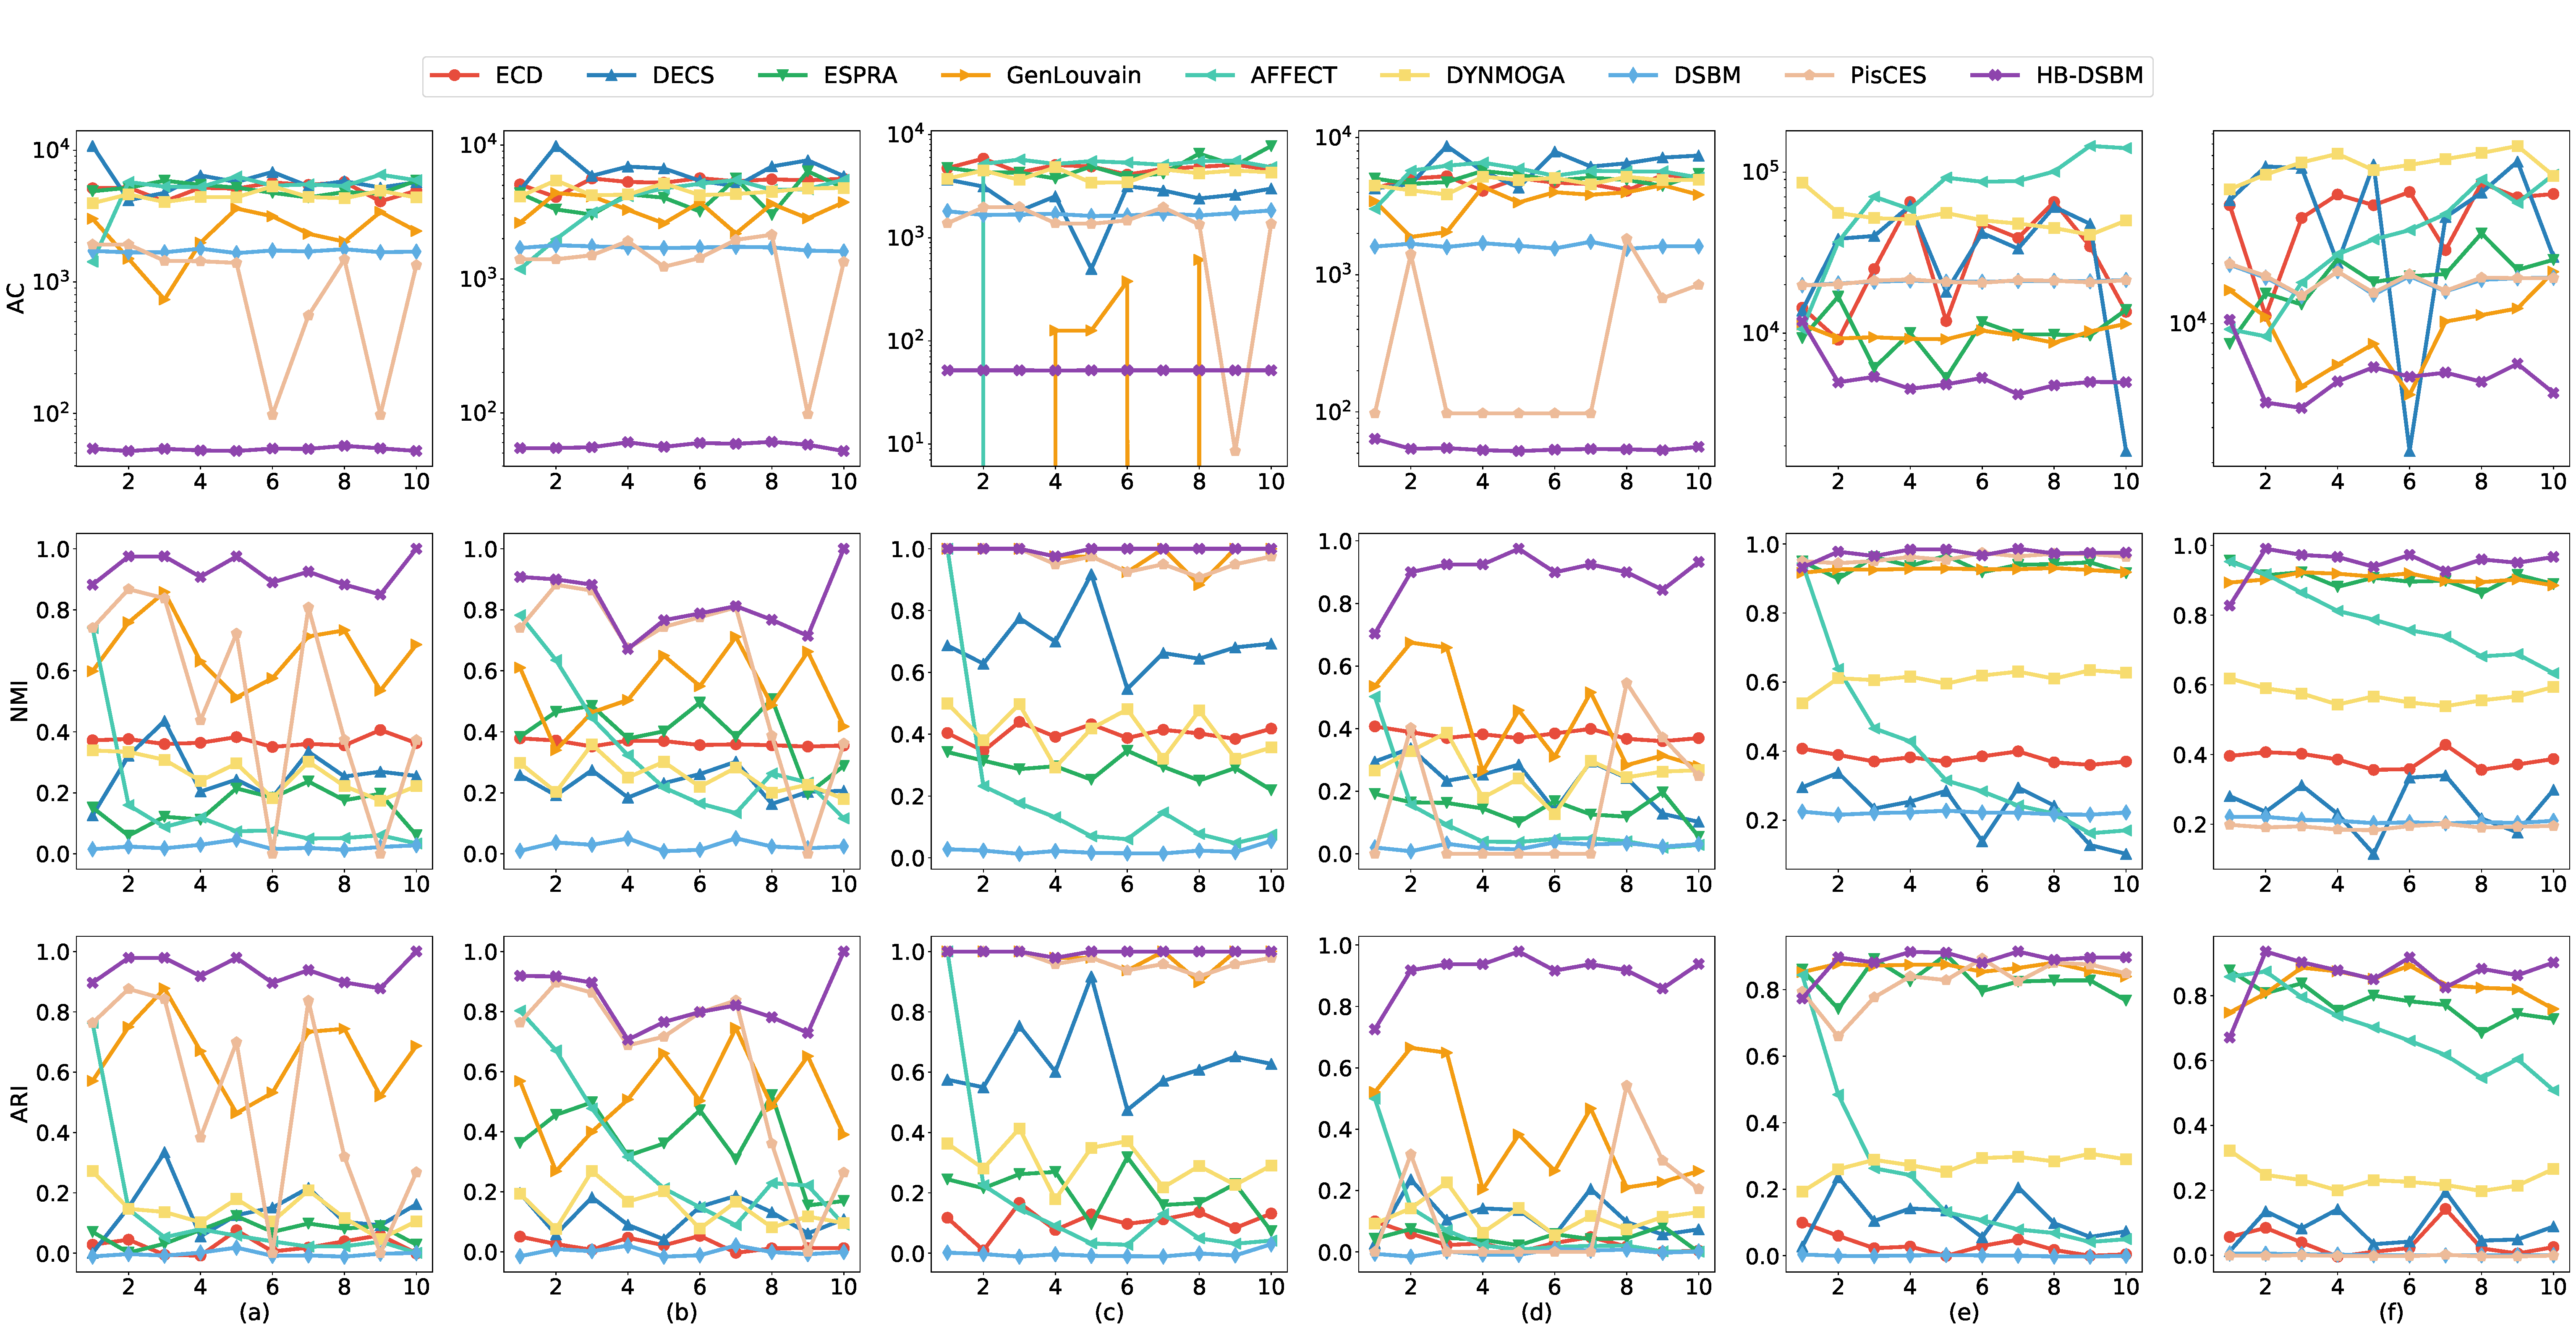
\includegraphics[width=0.9\textwidth]{figures/chap03/dsbm/newpics/generateData1223.pdf}
	\caption{生成数据集中的社团检测结果}
	\label{fig.4.2}
\end{figure}



真实世界数据集的实验结果如图~\ref{fig.4.4}。图~\ref{fig.4.4}中前三列为Kit-email数据按照不同时间间隔划分的结果,最后一列为DBLP数据集的社团检测结果。其展示了HB-DSBM对于真实世界数据的社团检测的优异能力,证明了本方法所刻画的节点演化异质性更加符合真实世界网络演化。值得注意的是,在第一个快照中,HB-DSBM的设计与静态随机块模型一致,因此本方法的优势在第一个快照并不明显,而随着时间推移,HB-DSBM对动态网络的建模优势逐渐显现。



\begin{figure}[htbp]
	\centering
	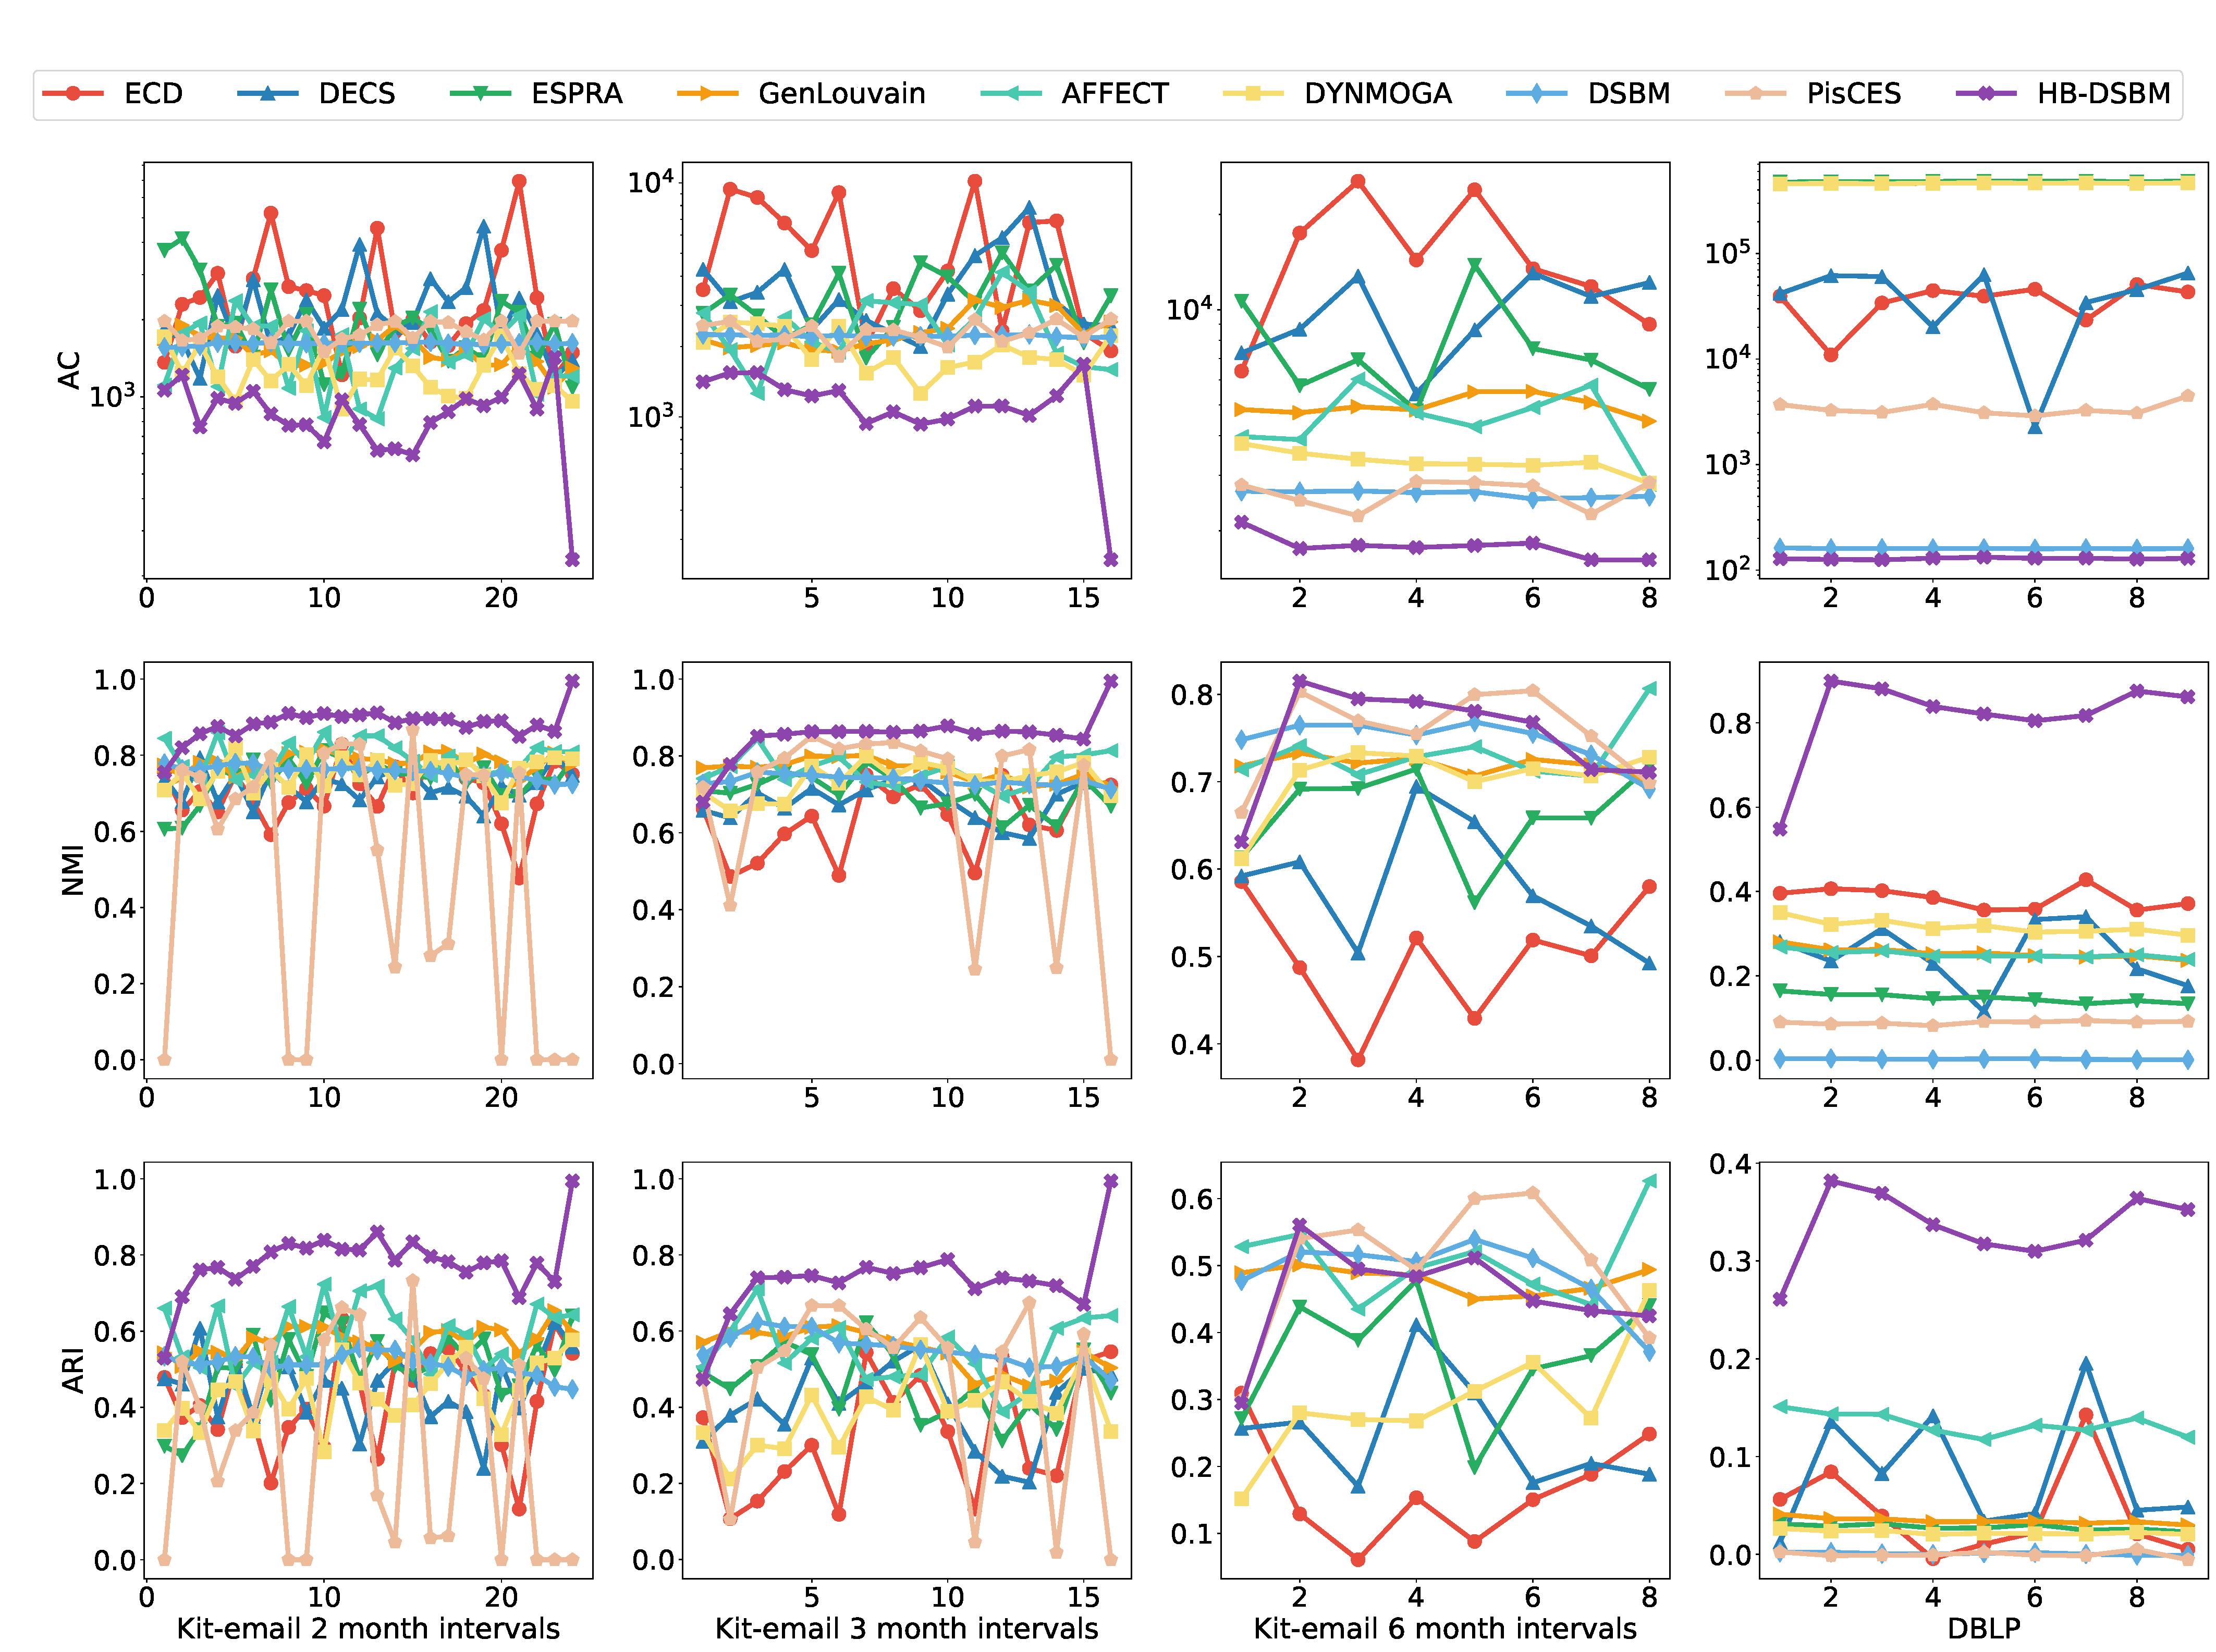
\includegraphics[width=0.9\textwidth]{figures/chap03/dsbm/newpics/realData1223.pdf}
	\caption{真实世界数据的社团检测结果}
	\label{fig.4.4}
\end{figure}




\subsection{社团演化分析}


社团演化方面,本节分别针对生成数据1、生成数据2以及DBLP数据进行了社团演化的可视化展示,如图~\ref{fig:SankeyFacetnet}~\ref{fig:SankeyAsonamMS}和图~\ref{fig:SankeyDBLP}所示,其中第一个GroundTruth代表社团真相。需要注意的是,由于ESPRA和AFFECT在生成数据2与DBLP数据中的社团演化效果较差,因此图中进行了省略。由图中可以看出,HB-DSBM能够准确的刻画动态网络的社团演化,且对于复杂的社团演化行为均具有较好的刻画能力。而DSBM由于缺少节点演化异质性假设,因此其难以建模复杂的社团演化行为,而其余方法如PisCES、DYNMOGA等由于模型设计的问题,呈现出了混乱的社团演化行为,难以正确刻画社团的演化,因此无法支撑对动态网络社团演化的分析。



\begin{figure}
	\centering
	\subfigure[GroundTruth]{
		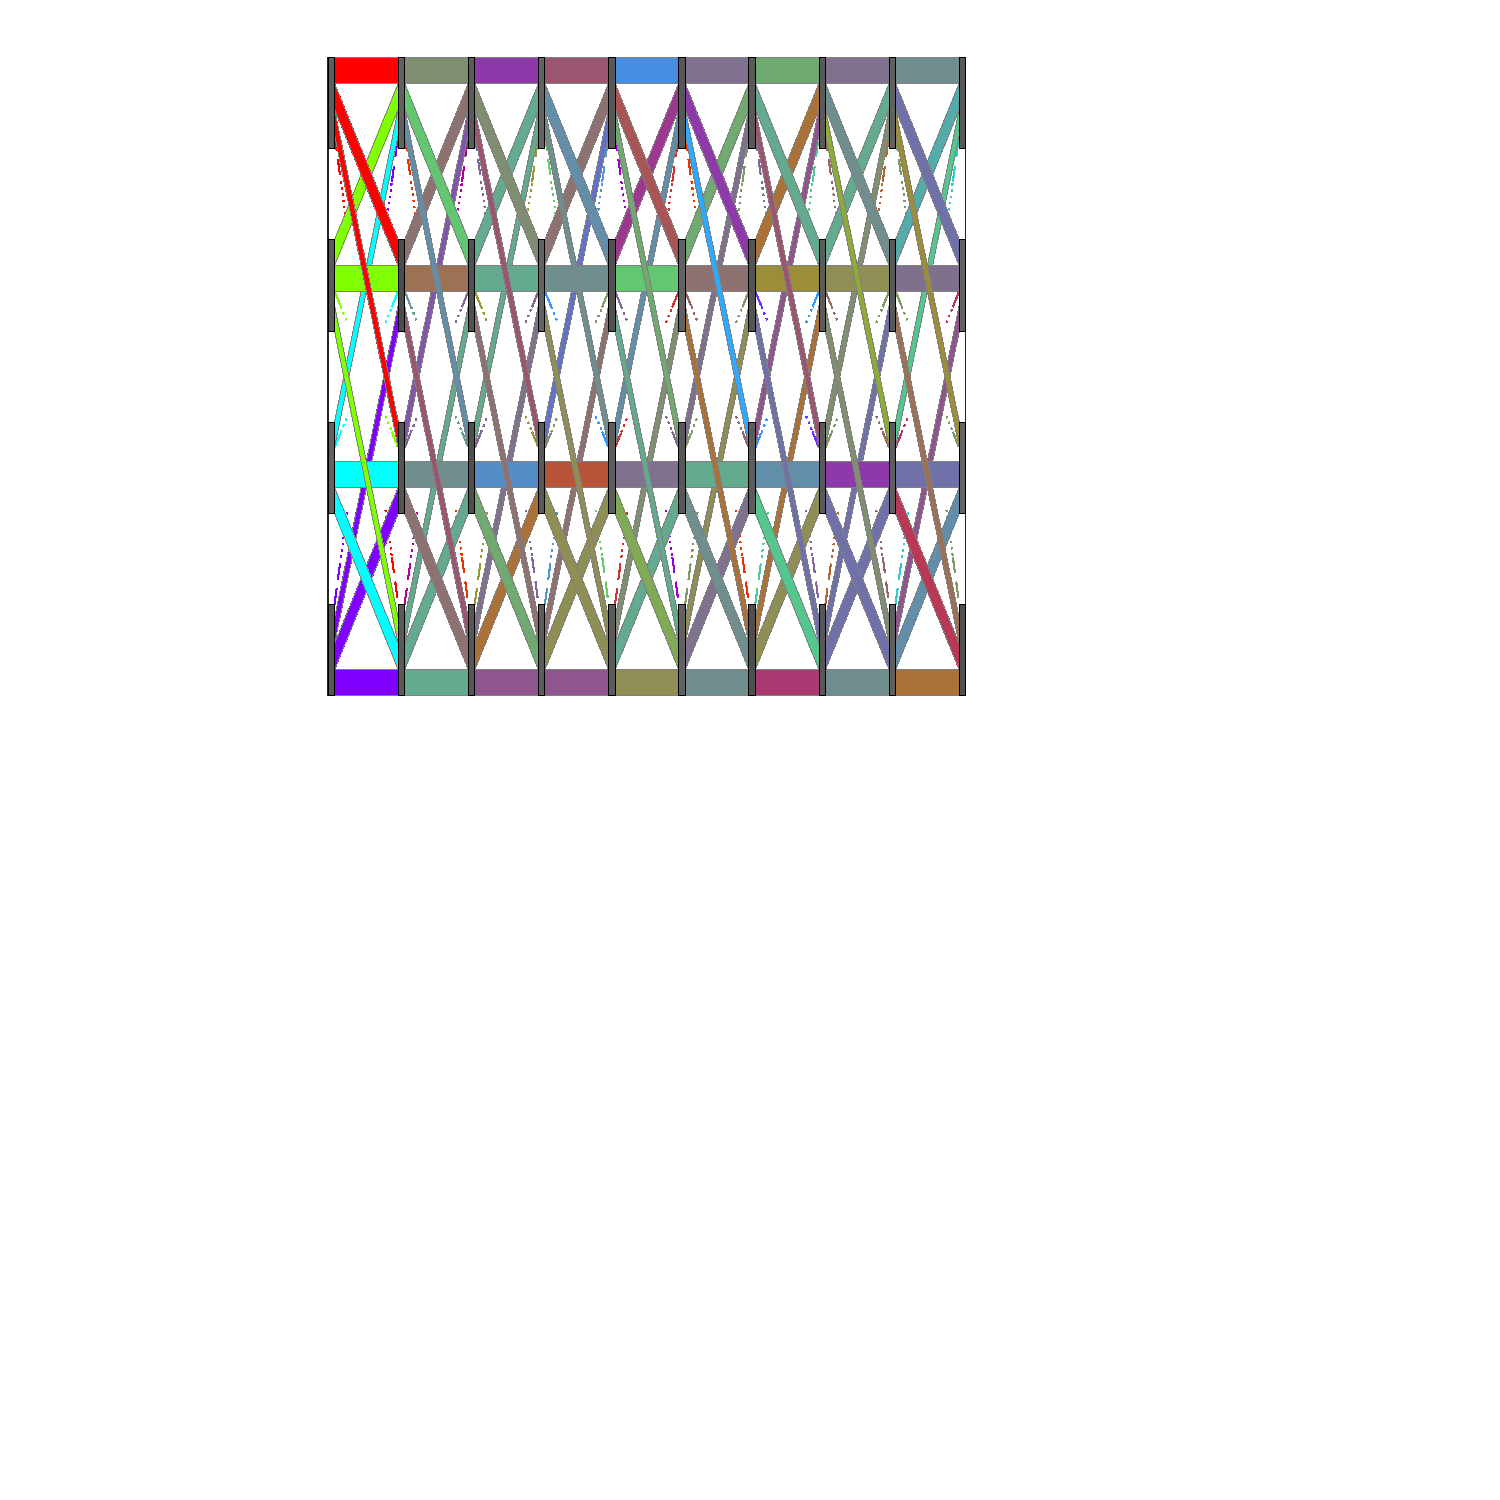
\includegraphics[width=.3\textwidth,height=.125\textwidth]{figures/chap03/dsbm/facetNetEvolution/groundTruth.pdf}
	}
	\subfigure[DSBM]{
		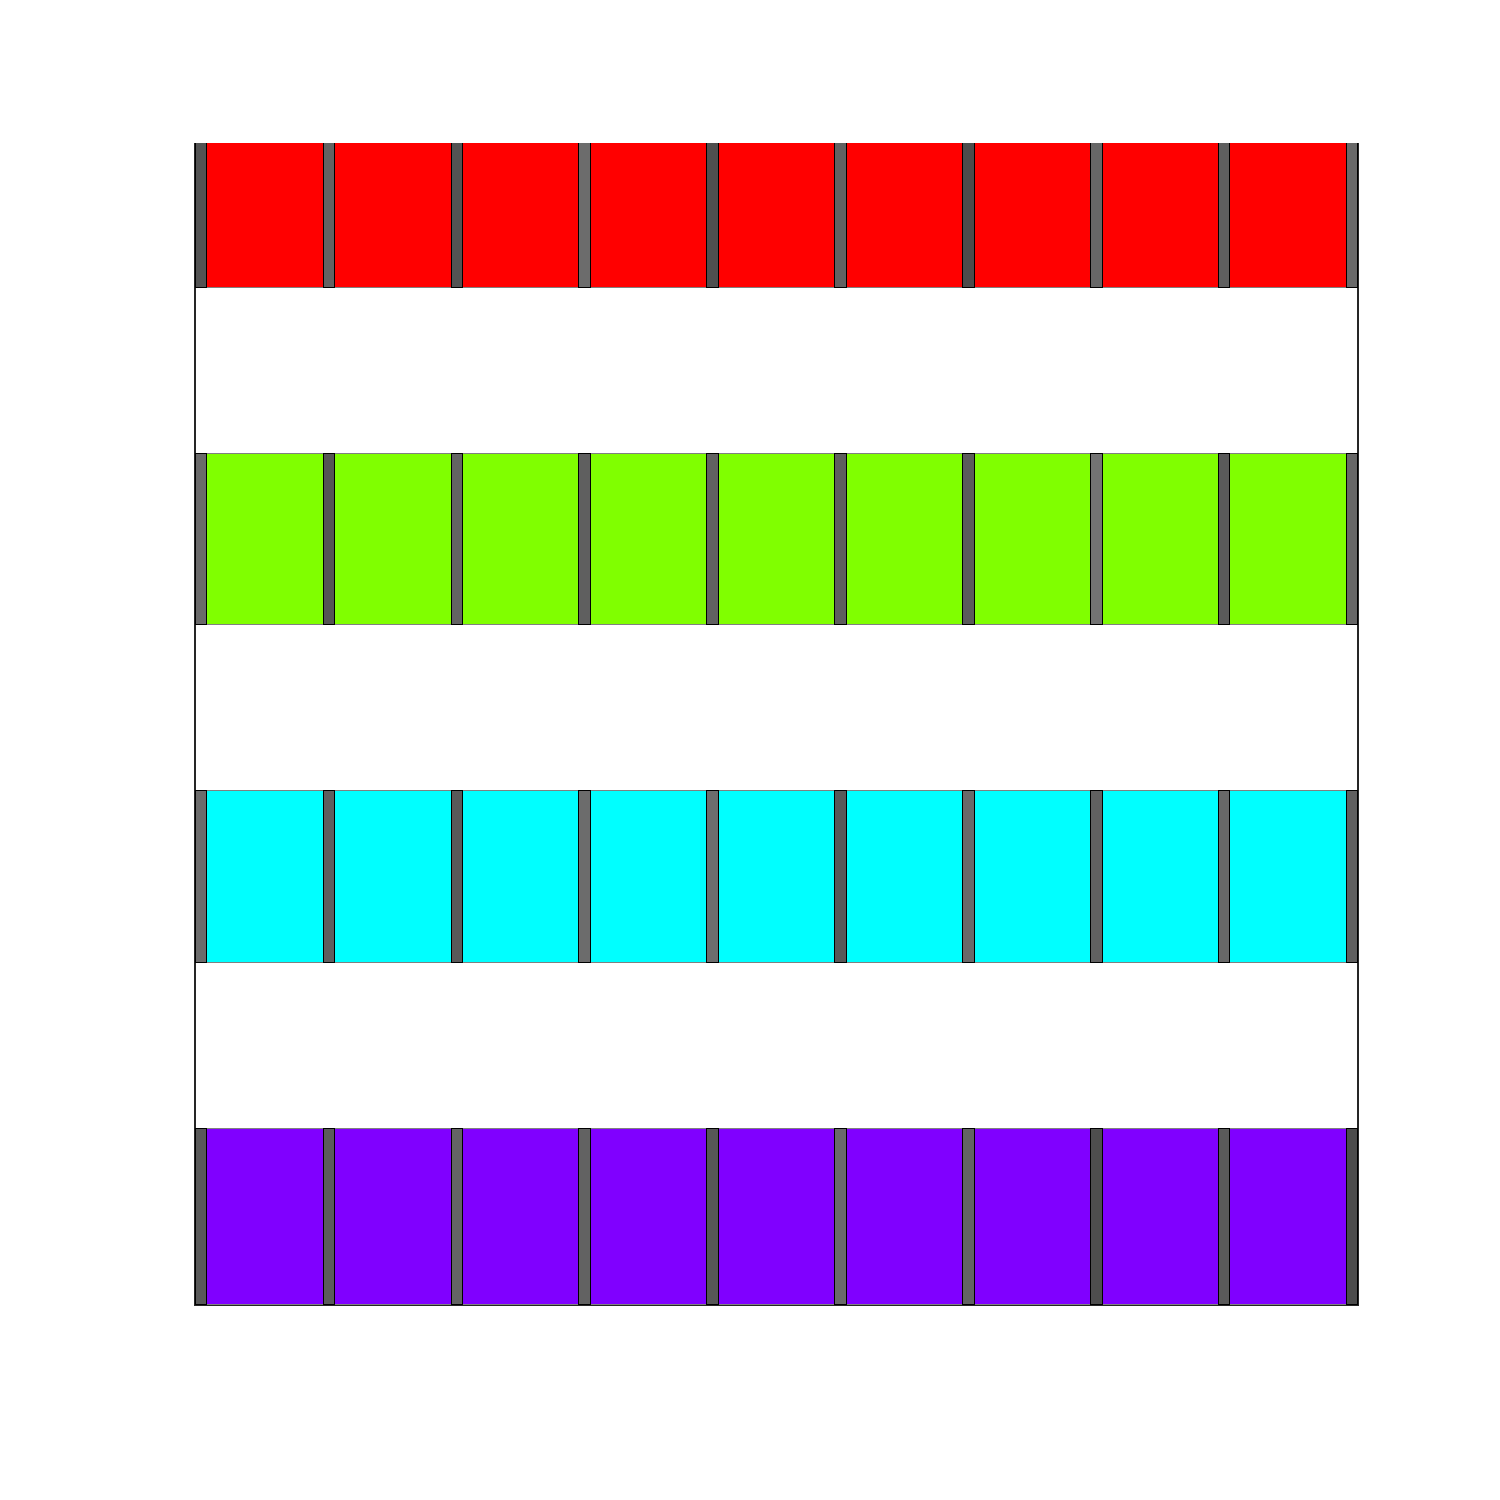
\includegraphics[width=.3\textwidth,height=.125\textwidth]{figures/chap03/dsbm/facetNetEvolution/DSBM.pdf}
	}
	\subfigure[HB-DSBM]{
		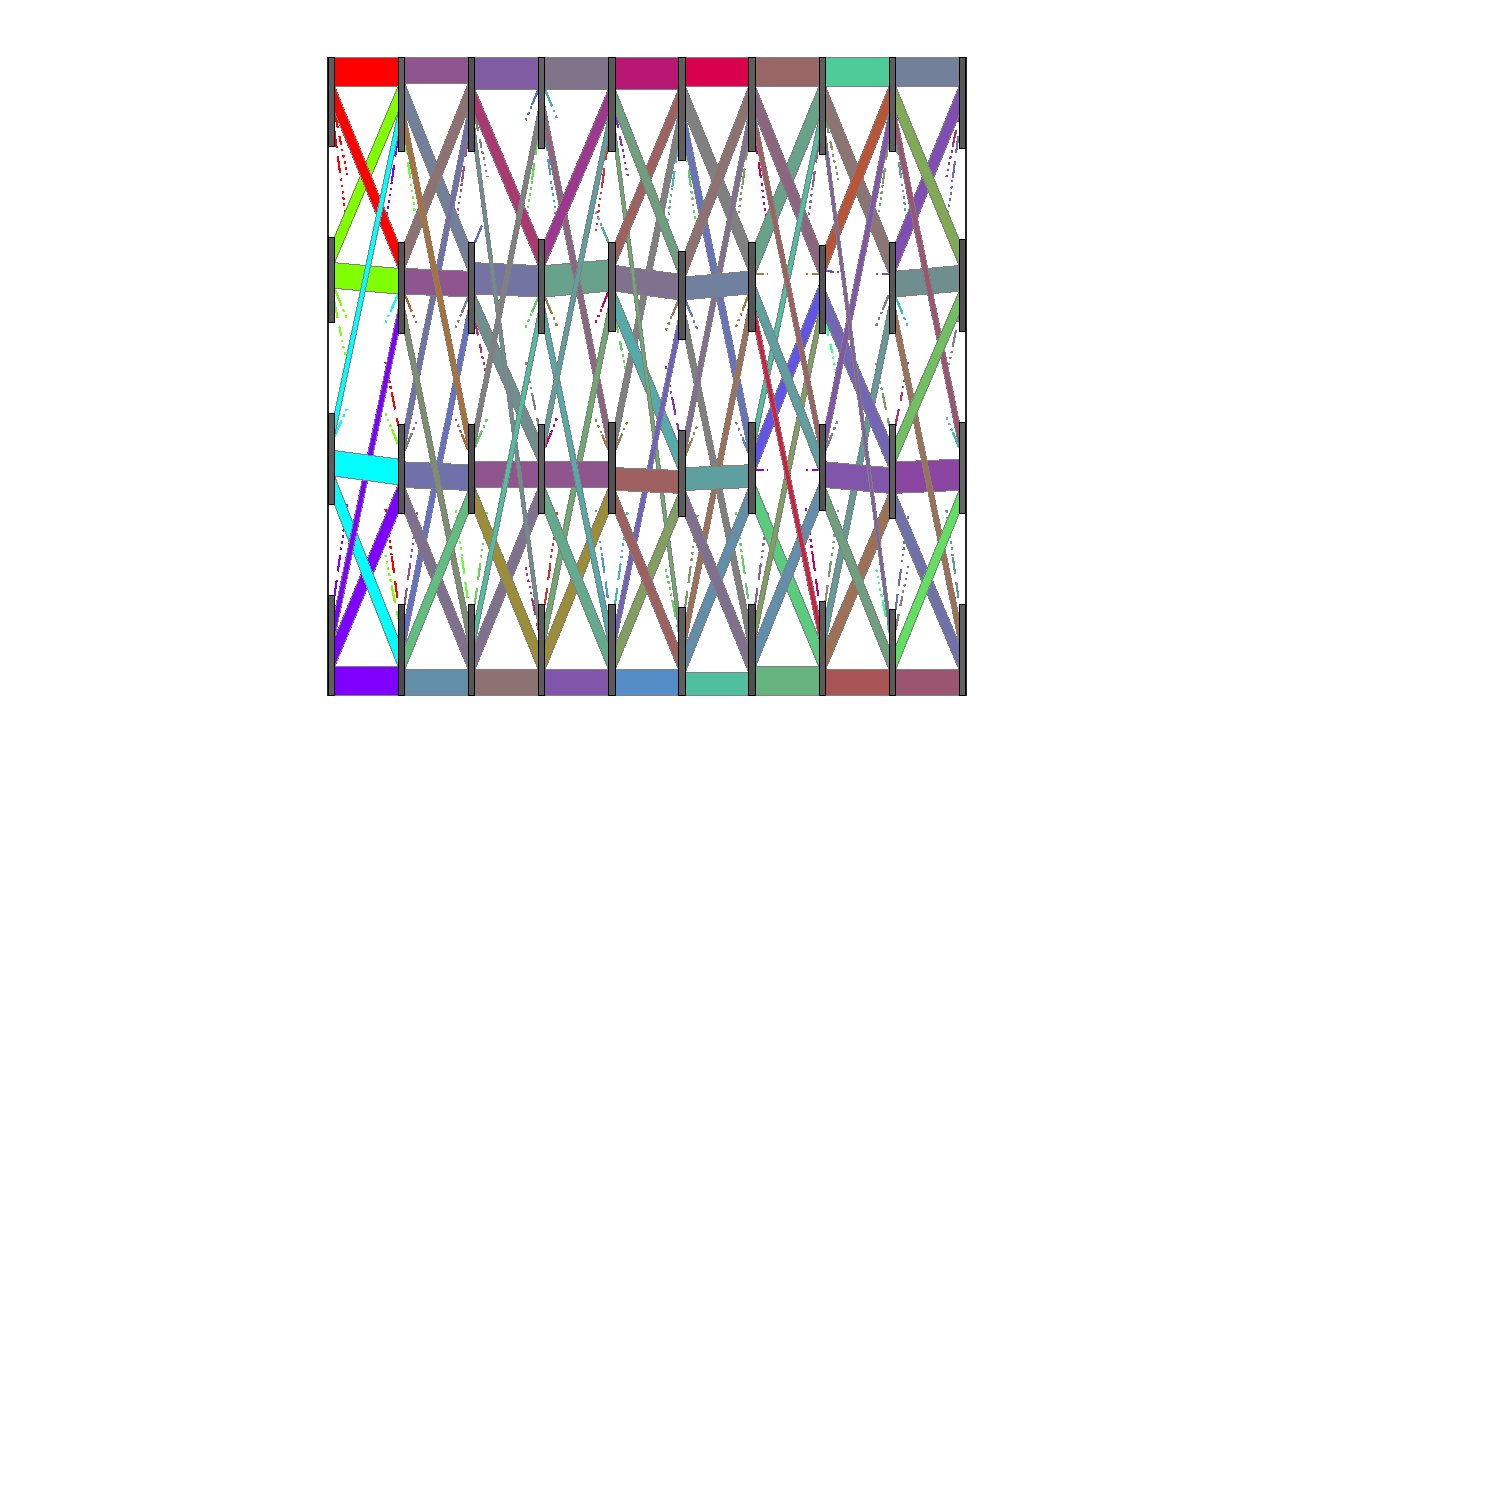
\includegraphics[width=.3\textwidth,height=.125\textwidth]{figures/chap03/dsbm/facetNetEvolution/HBDSBM.pdf}
	}
	\subfigure[GenLouvain]{
		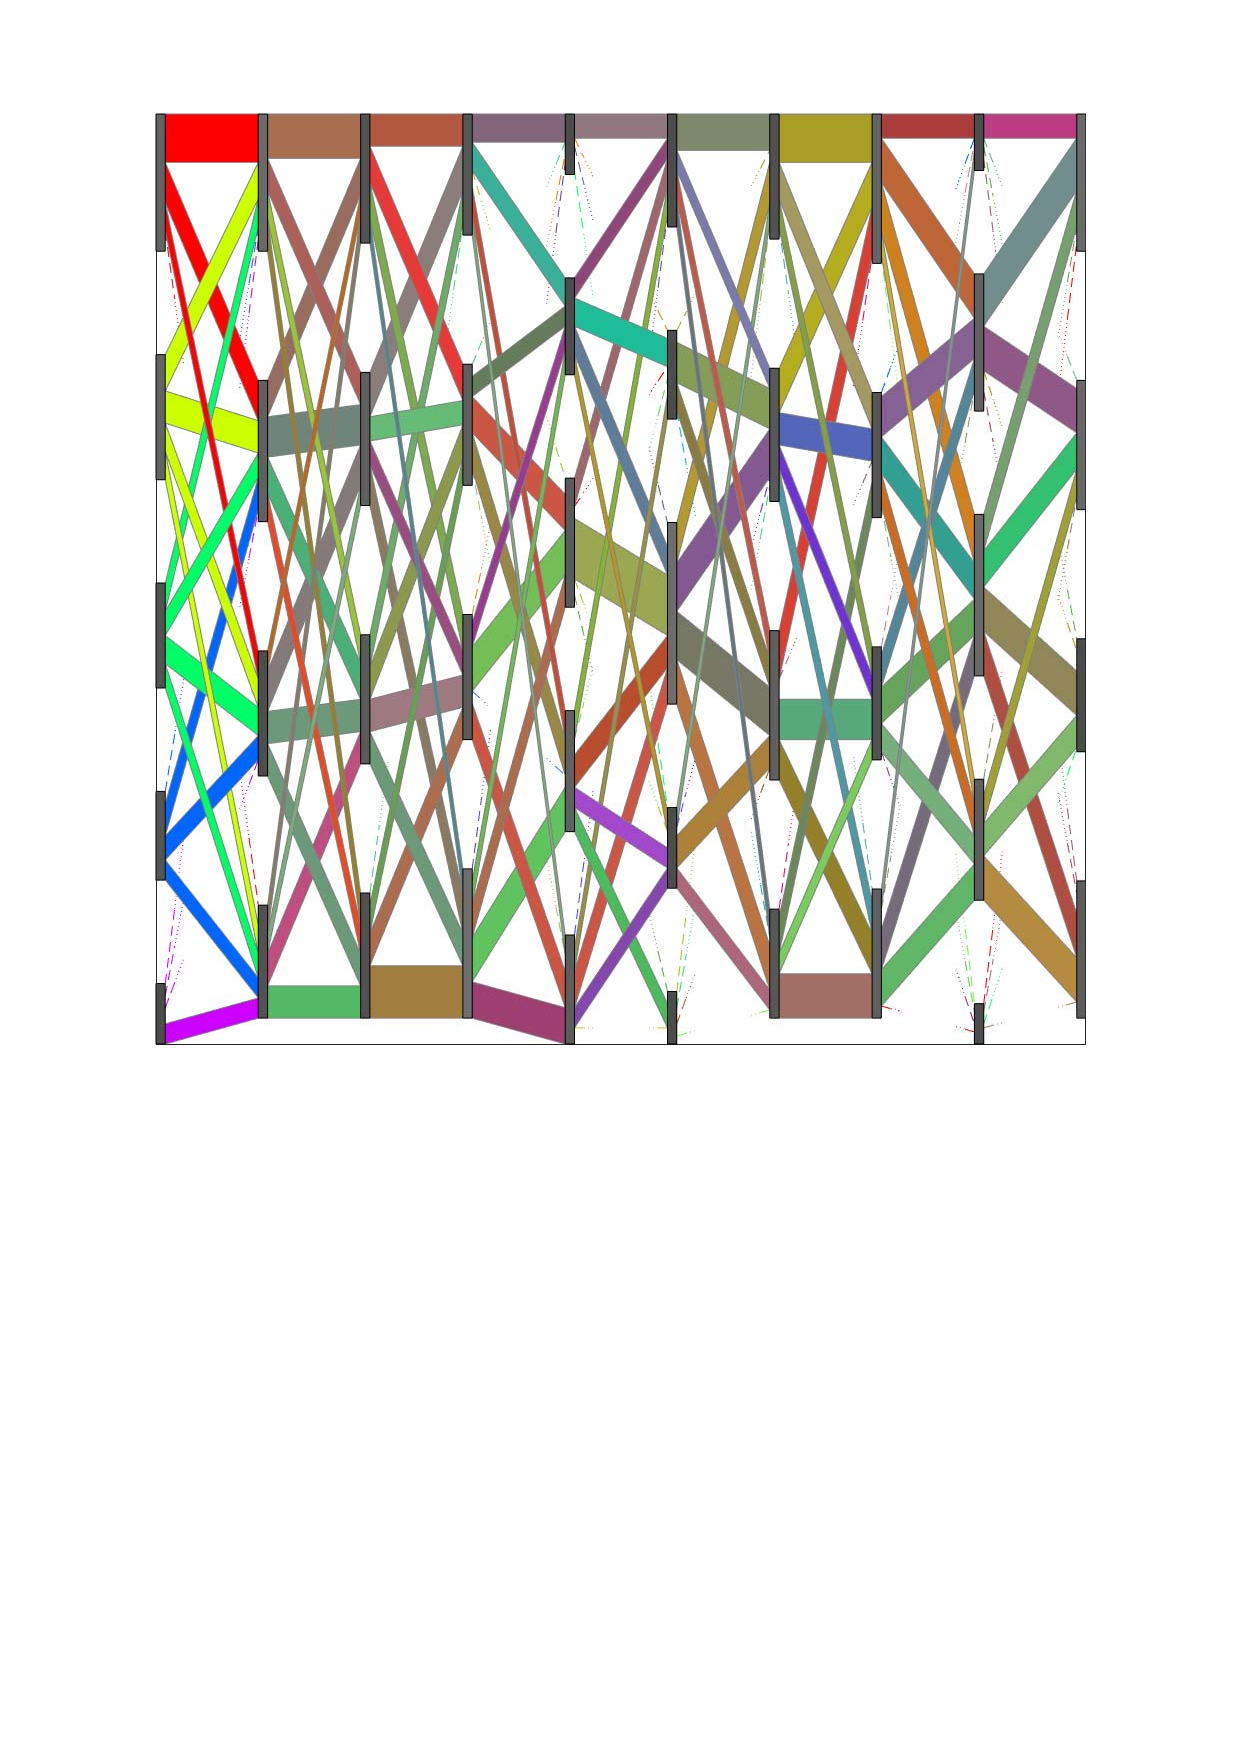
\includegraphics[width=.3\textwidth,height=.125\textwidth]{figures/chap03/dsbm/facetNetEvolution/gen.pdf}
	}
	\subfigure[PisCES]{
		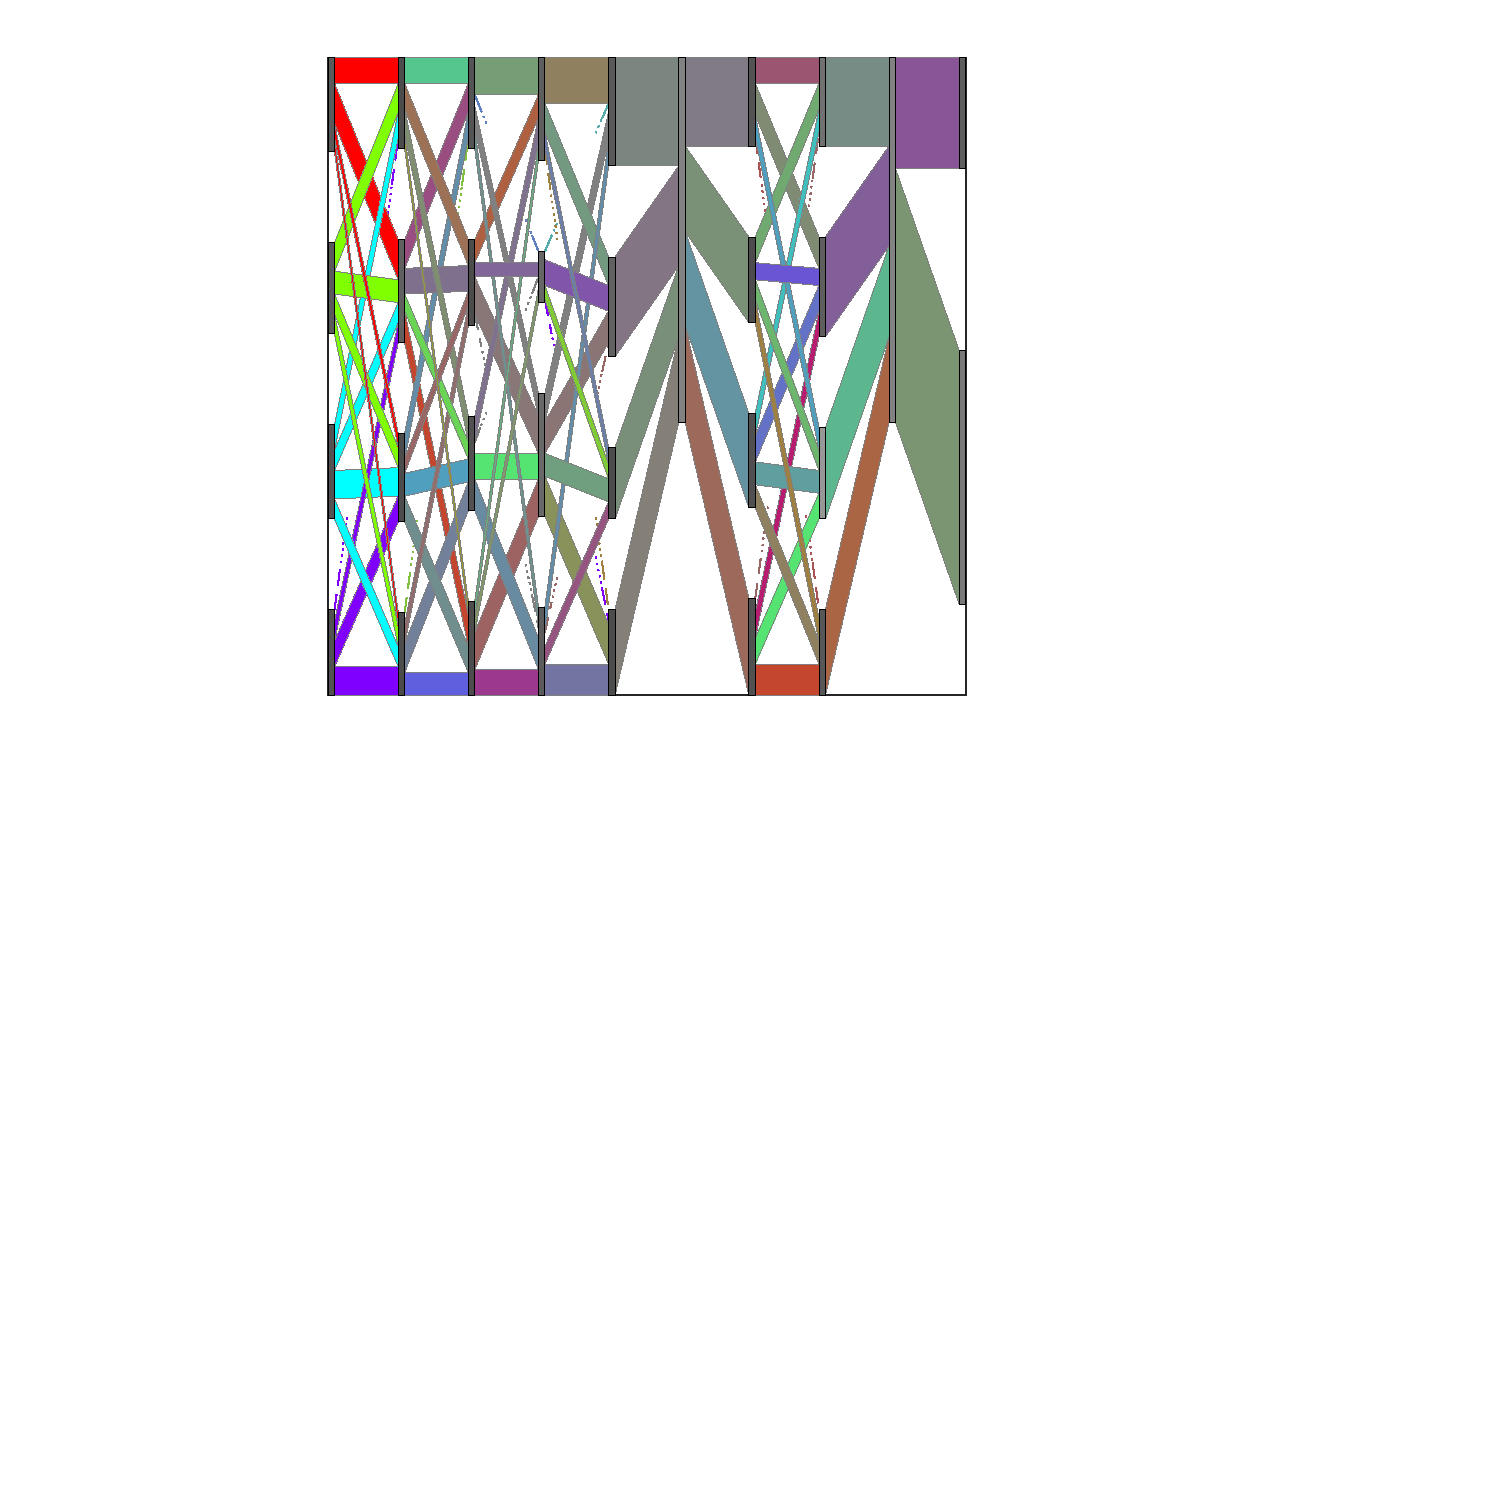
\includegraphics[width=.3\textwidth,height=.125\textwidth]{figures/chap03/dsbm/facetNetEvolution/PisCES.pdf}
	}
	\subfigure[DYNMOGA]{
		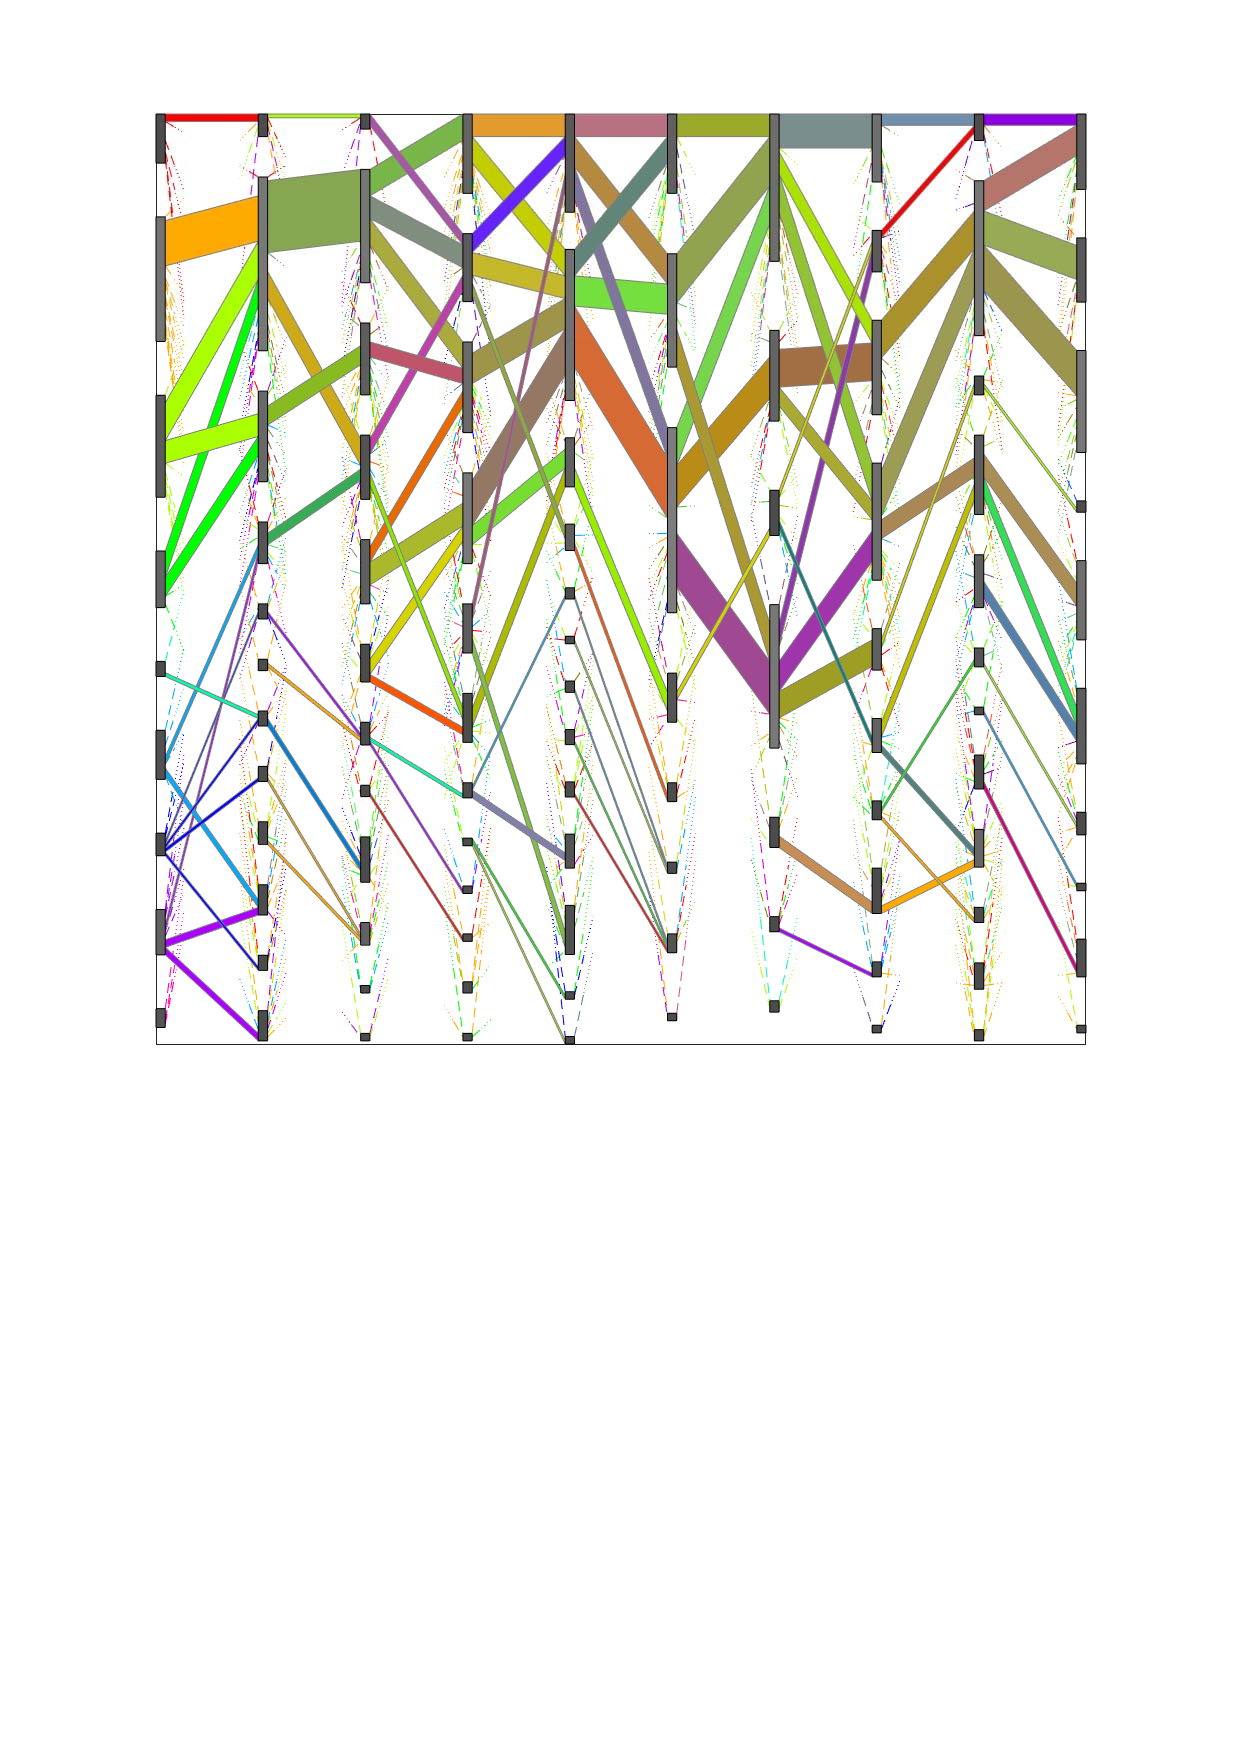
\includegraphics[width=.3\textwidth,height=.125\textwidth]{figures/chap03/dsbm/facetNetEvolution/dynmoga.pdf}
	}
	\subfigure[DECS]{
		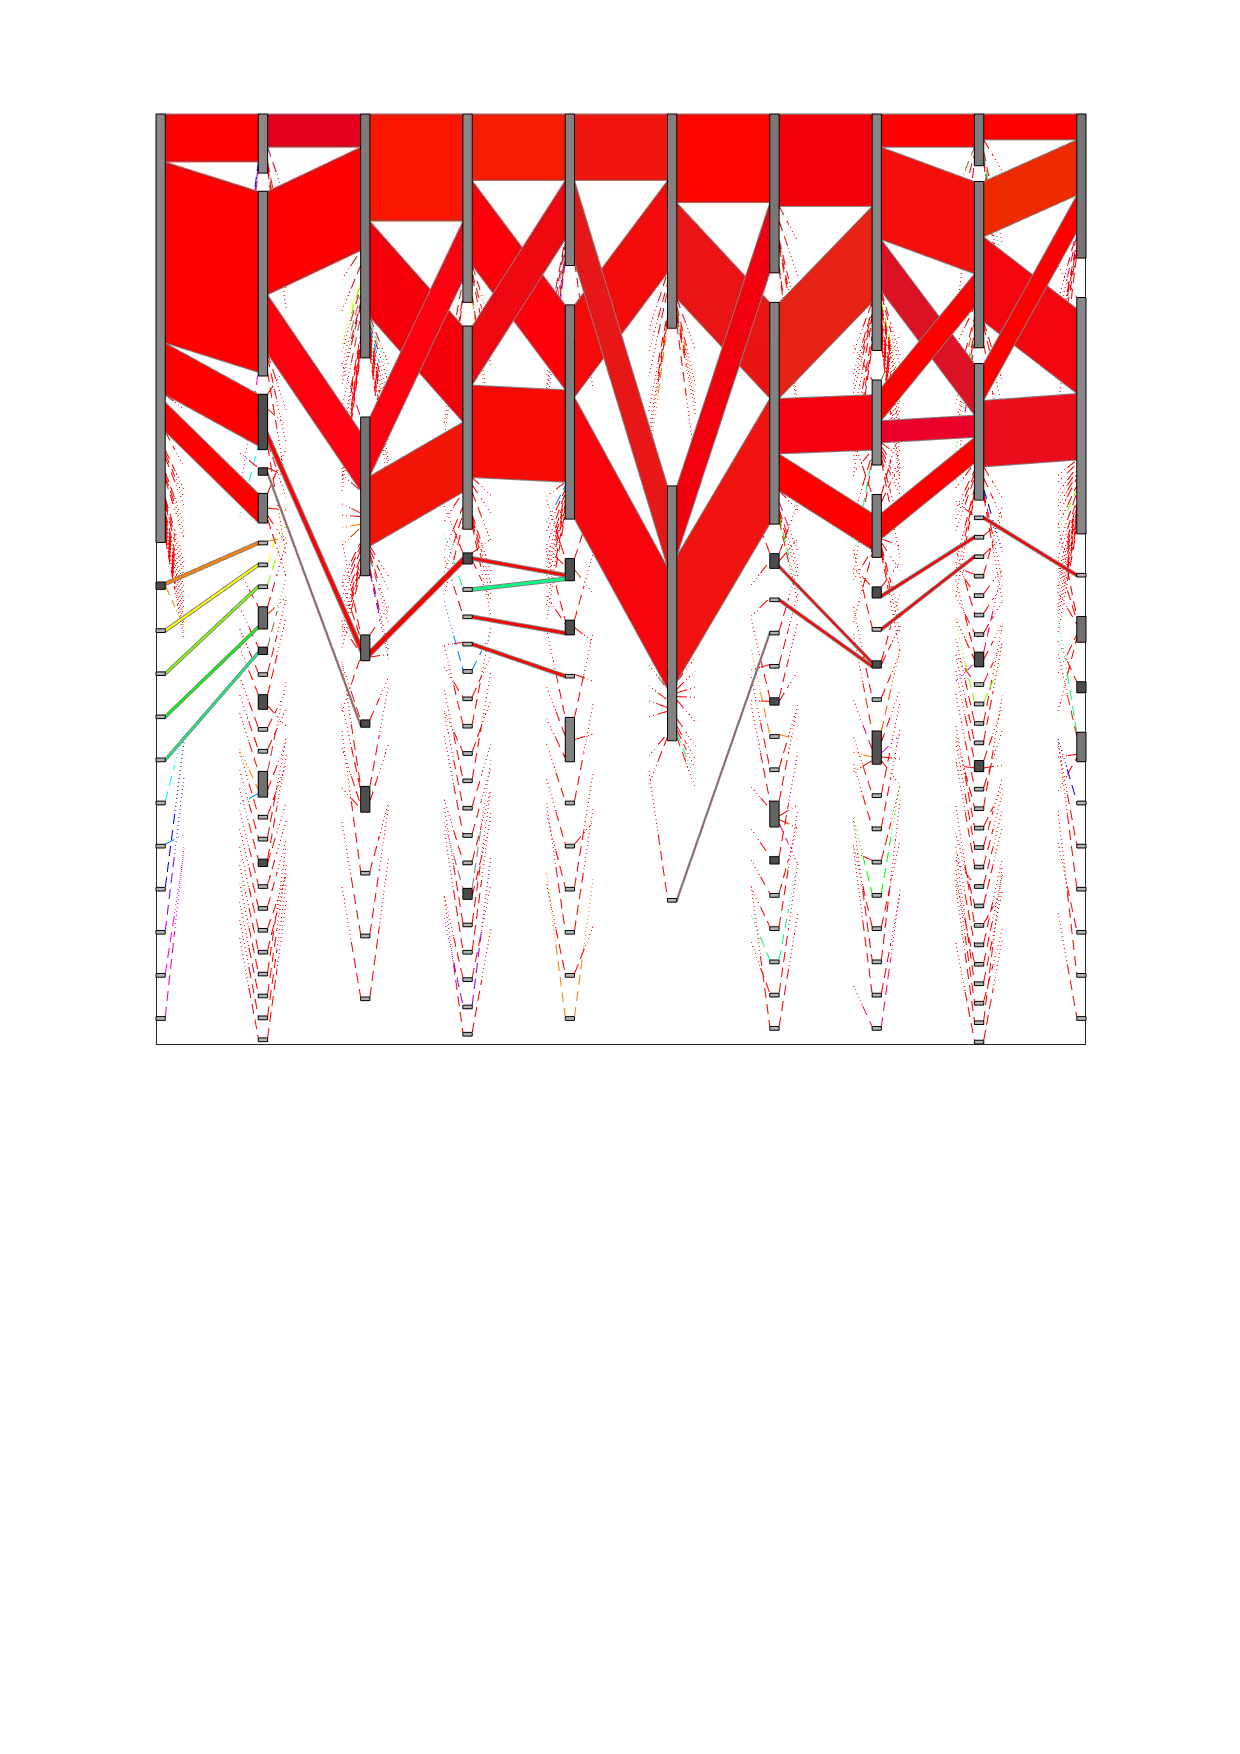
\includegraphics[width=.3\textwidth,height=.125\textwidth]{figures/chap03/dsbm/facetNetEvolution/DECS.pdf}
	}
	\subfigure[ESPRA]{
		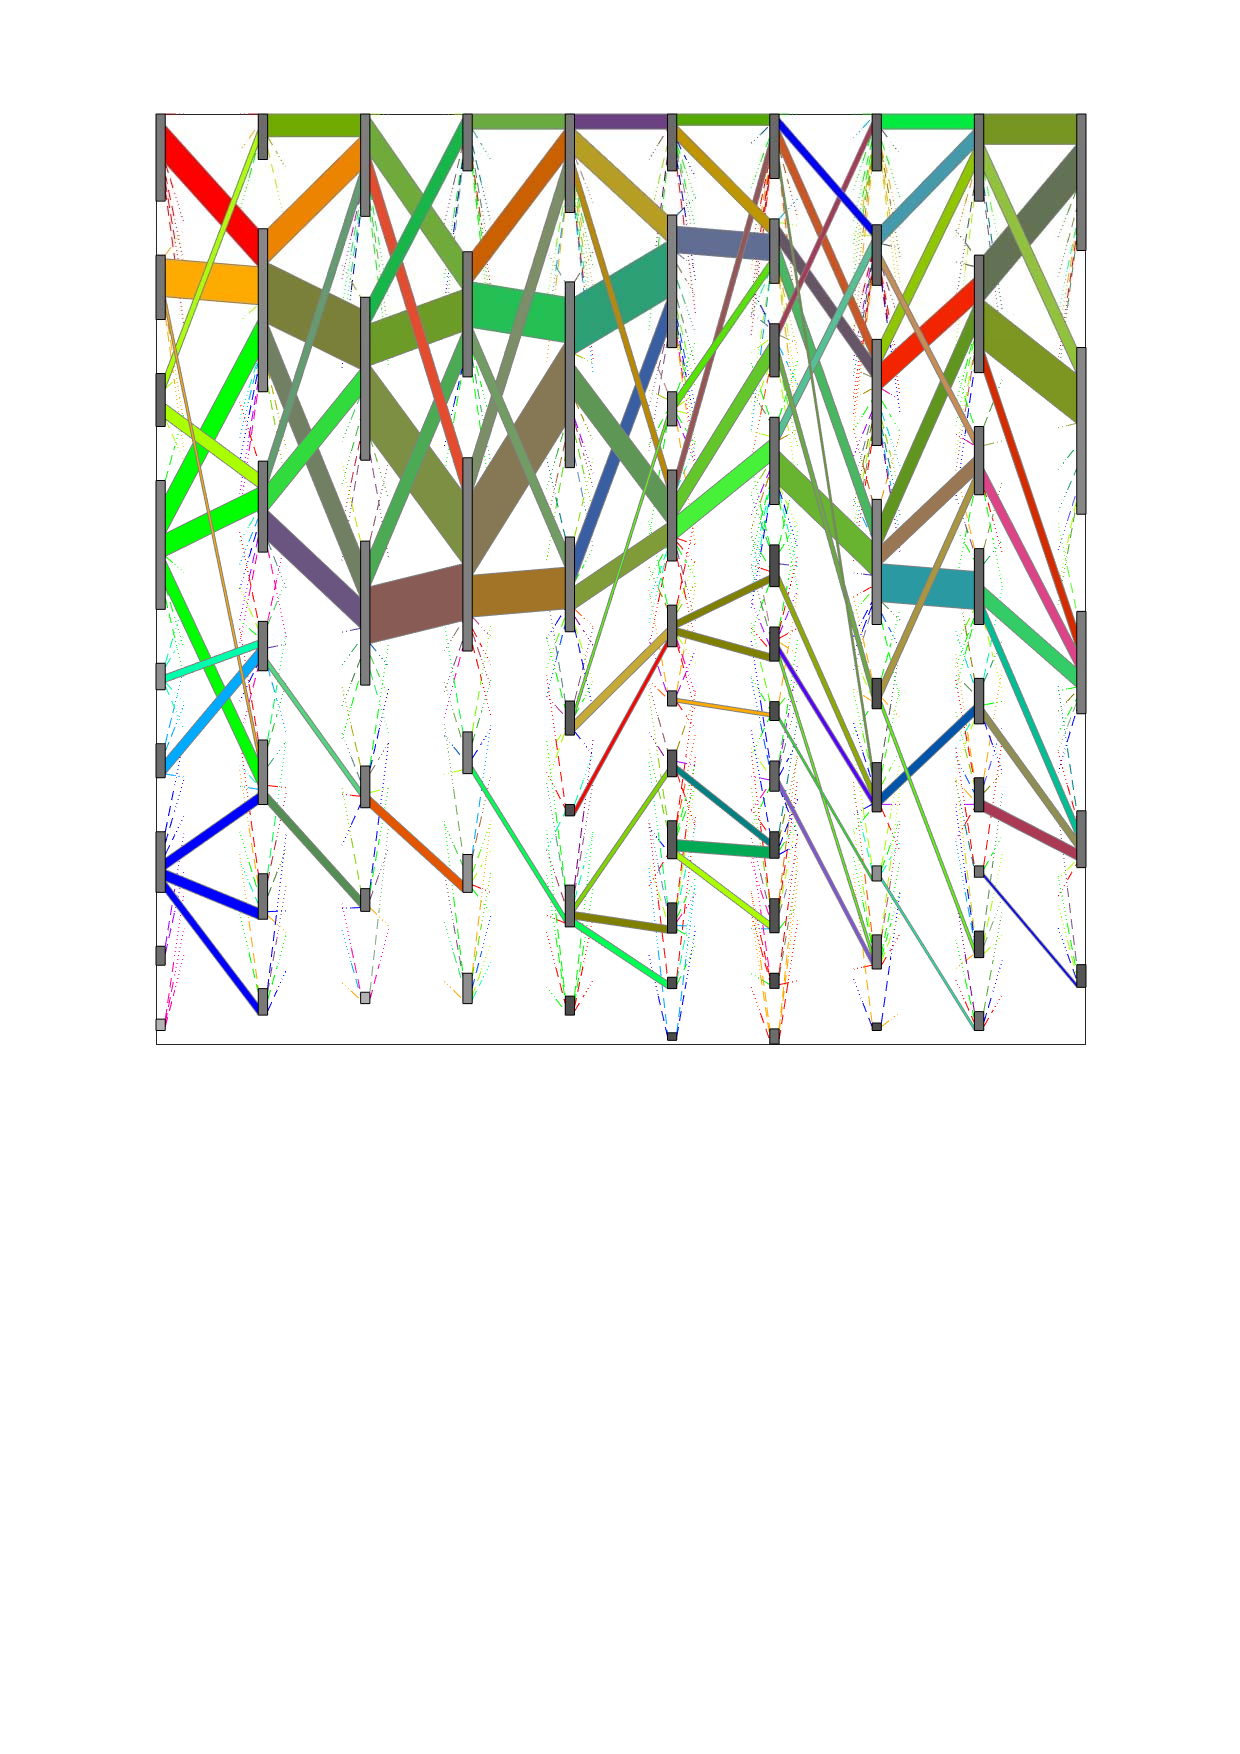
\includegraphics[width=.3\textwidth,height=.125\textwidth]{figures/chap03/dsbm/facetNetEvolution/espra.pdf}
	}
	\subfigure[AFFECT]{
		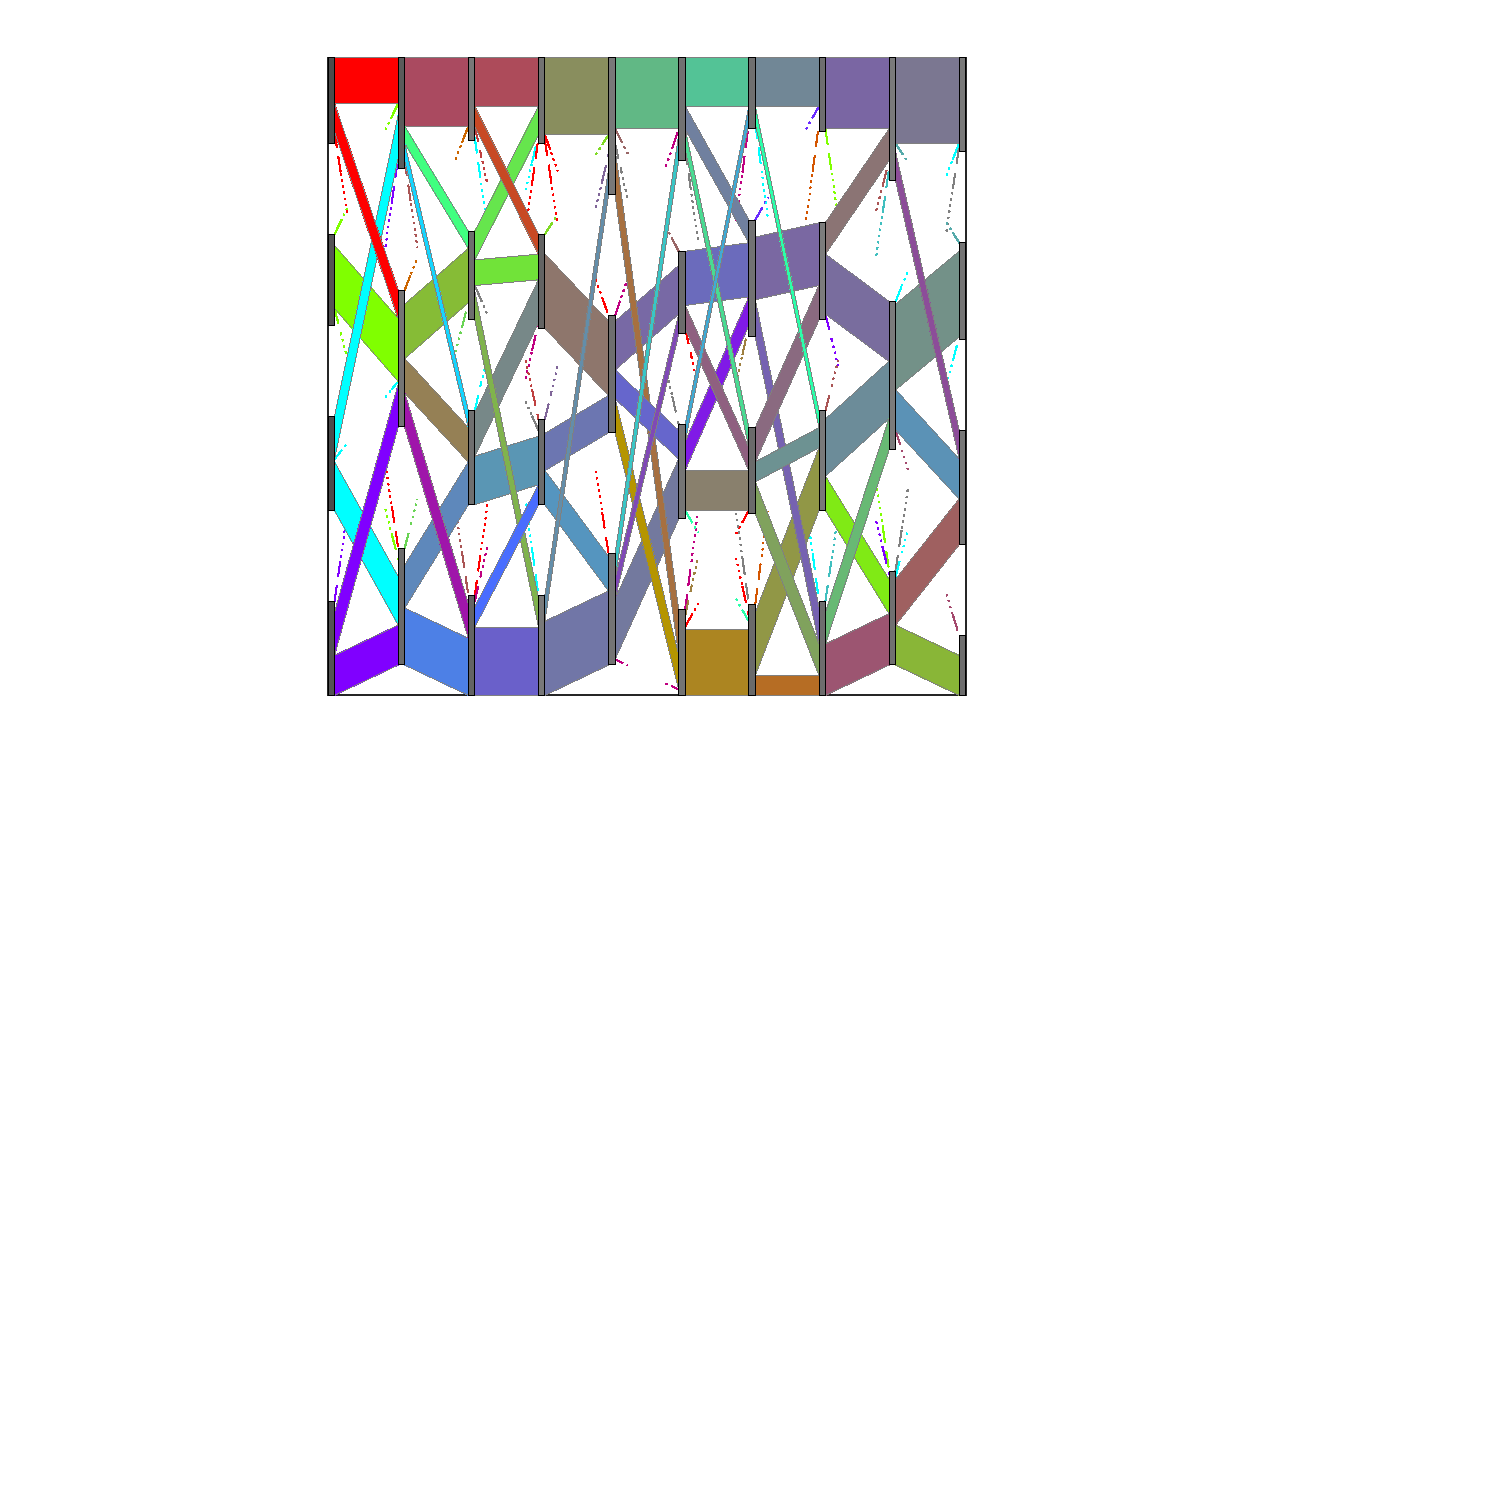
\includegraphics[width=.3\textwidth,height=.125\textwidth]{figures/chap03/dsbm/facetNetEvolution/affect.pdf}
	}
	\caption{生成数据1中参数为$\sigma = 5$, $nC = 9$ and $aD = 20$的社团演化桑基图}
	\label{fig:SankeyFacetnet}
	%  \vspace{-0.5cm}
\end{figure}



 \begin{figure}
	\centering
	\subfigure[GroundTruth]{
		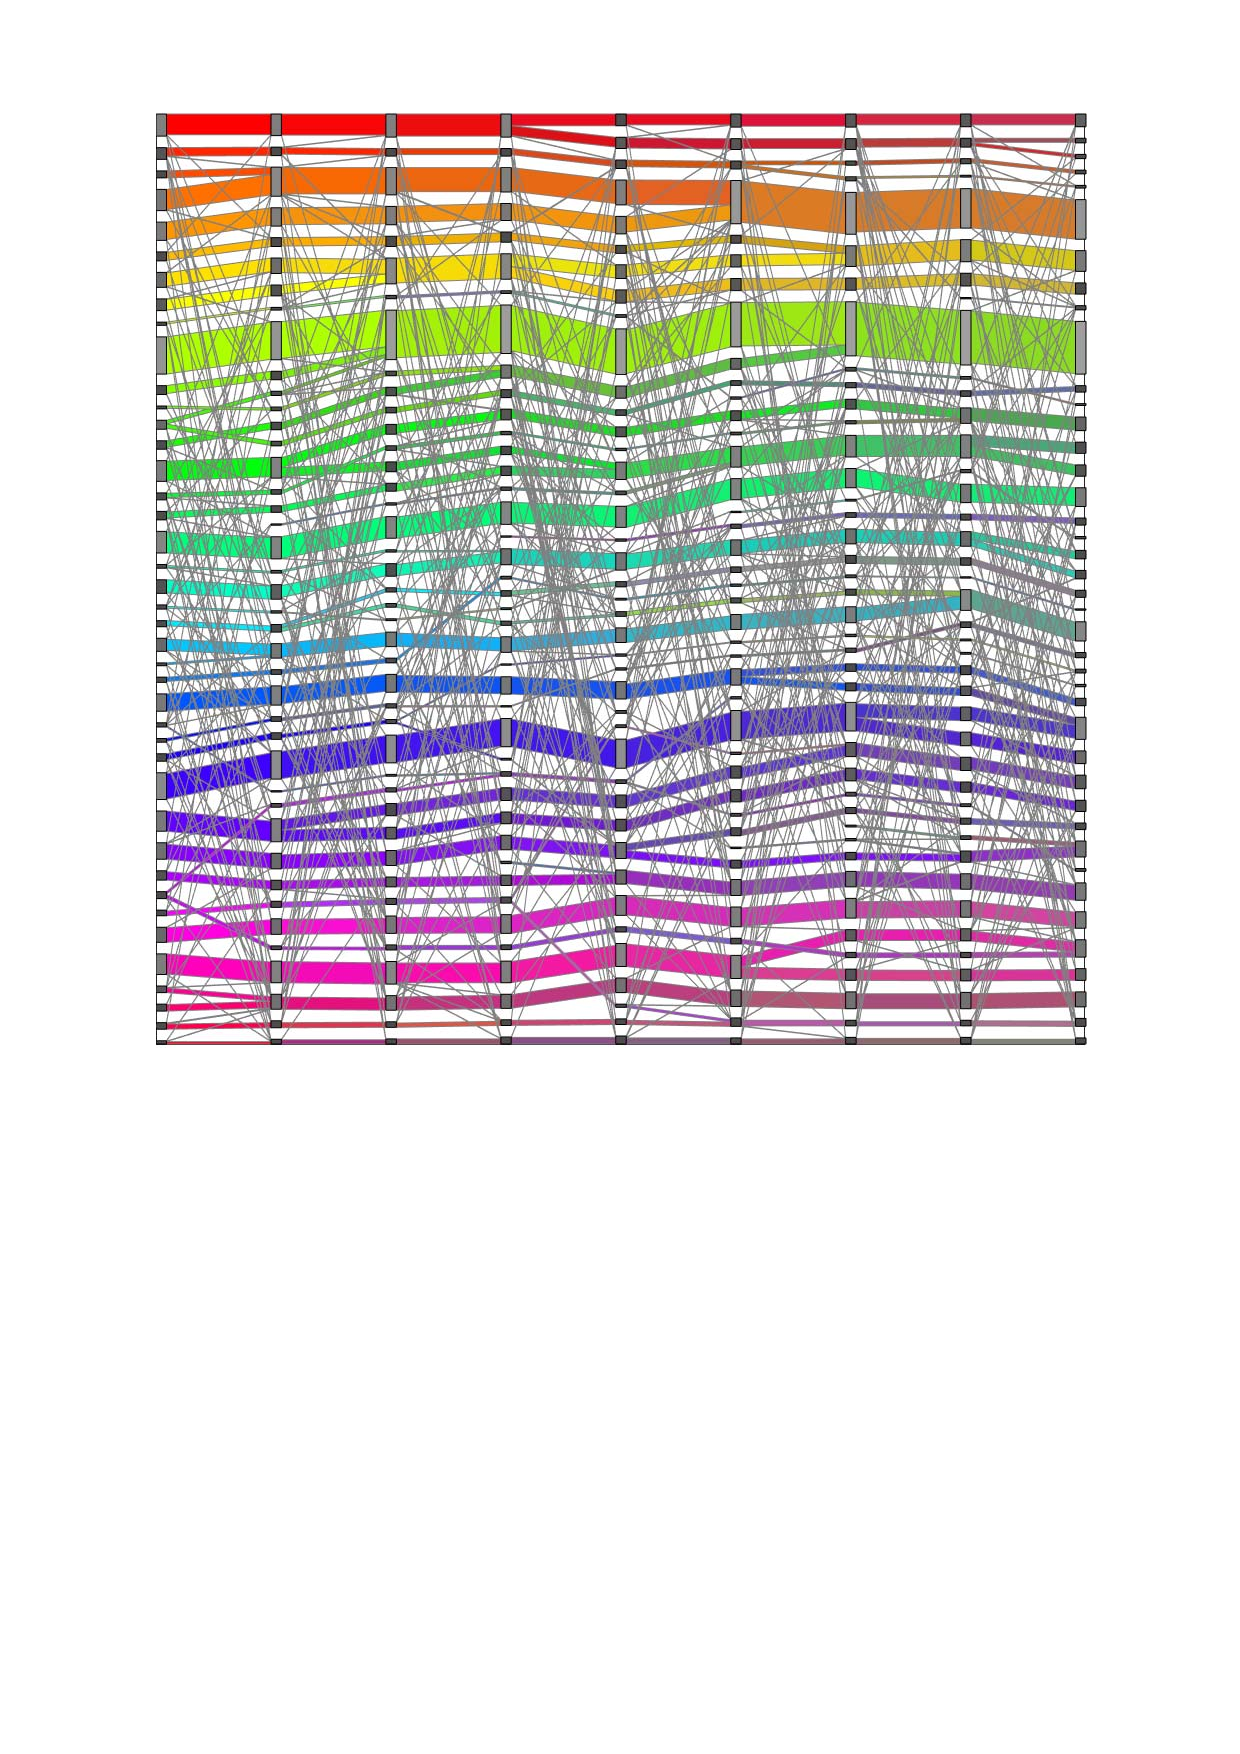
\includegraphics[width=.3\textwidth,height=.15\textwidth]{figures/chap03/dsbm/ASONEMmsEvolution/1GroundTruth.pdf}
	}
	\subfigure[DSBM]{
		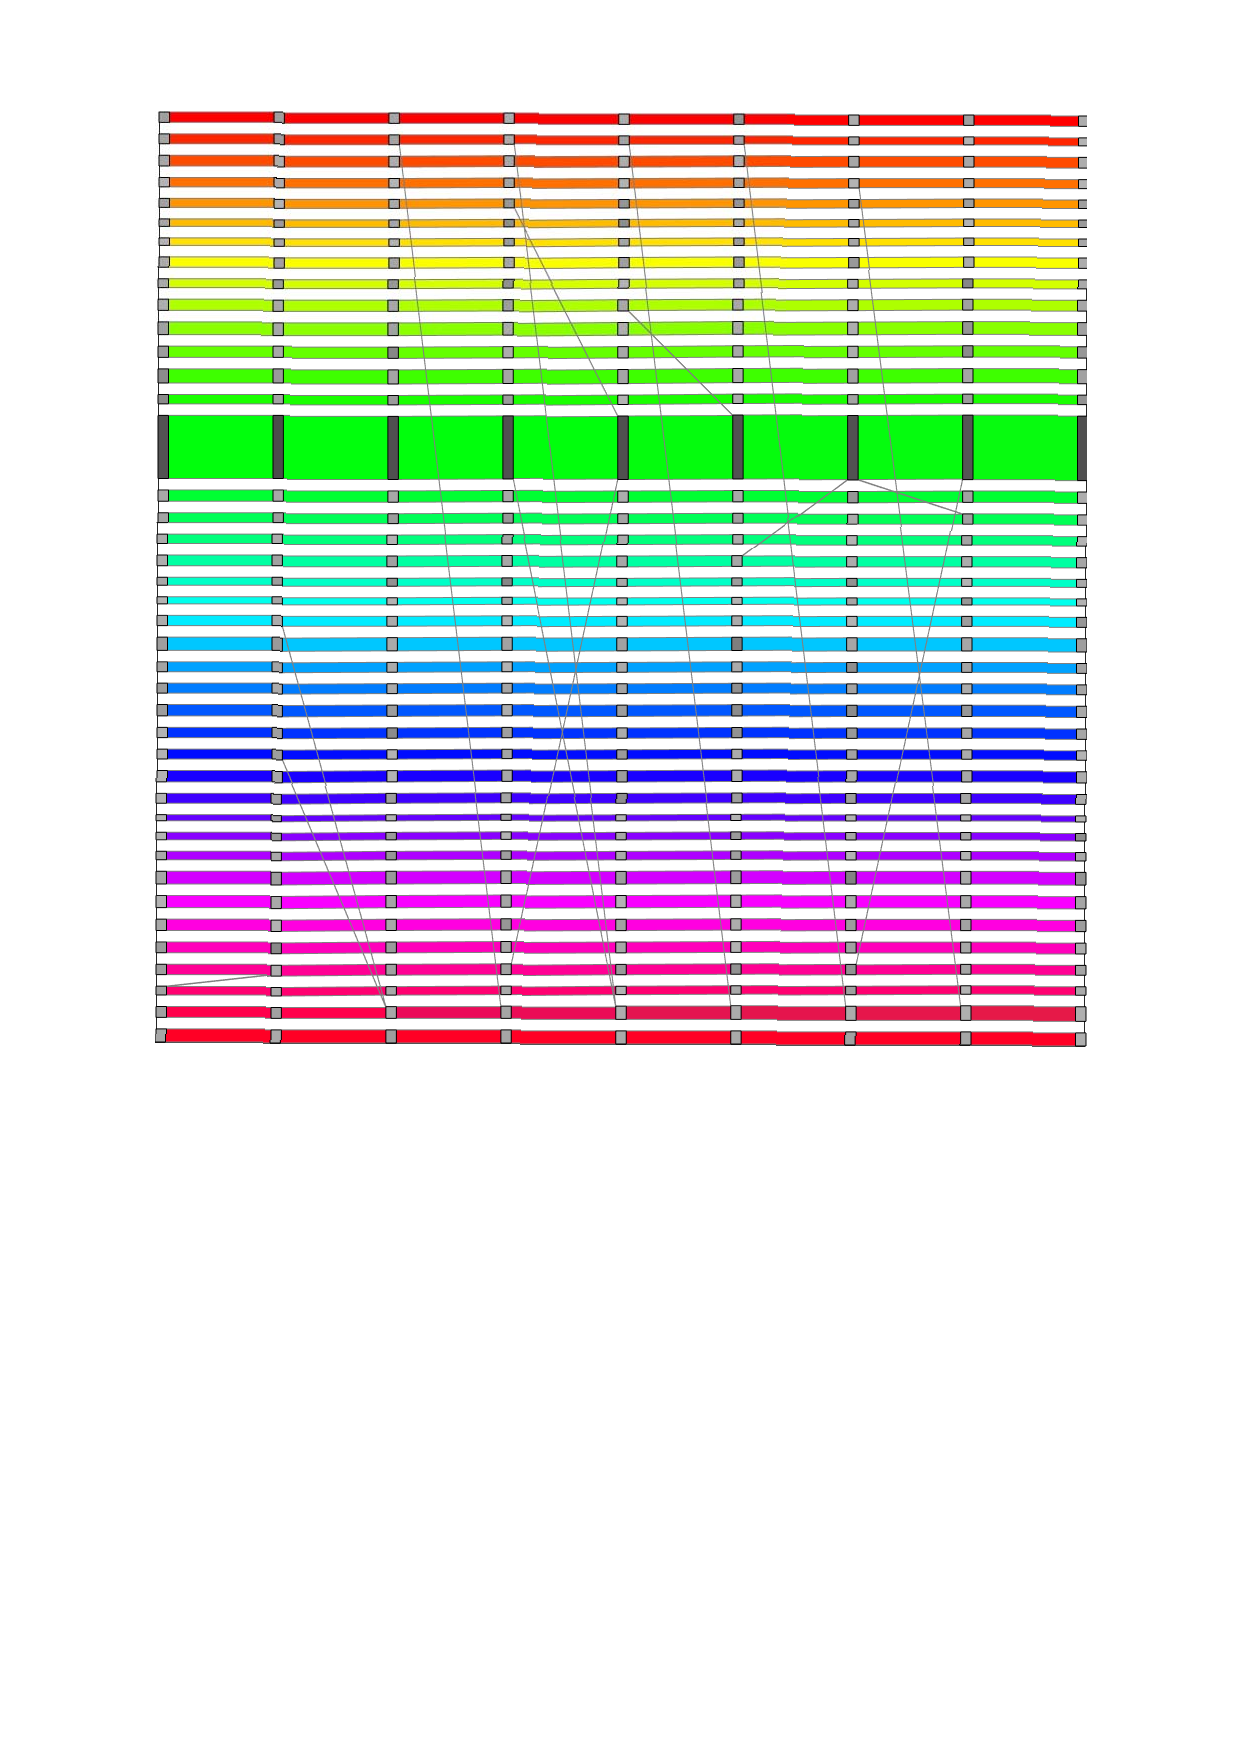
\includegraphics[width=.3\textwidth,height=.15\textwidth]{figures/chap03/dsbm/ASONEMmsEvolution/1DSBM.pdf}
	}
	\subfigure[HB-DSBM]{
		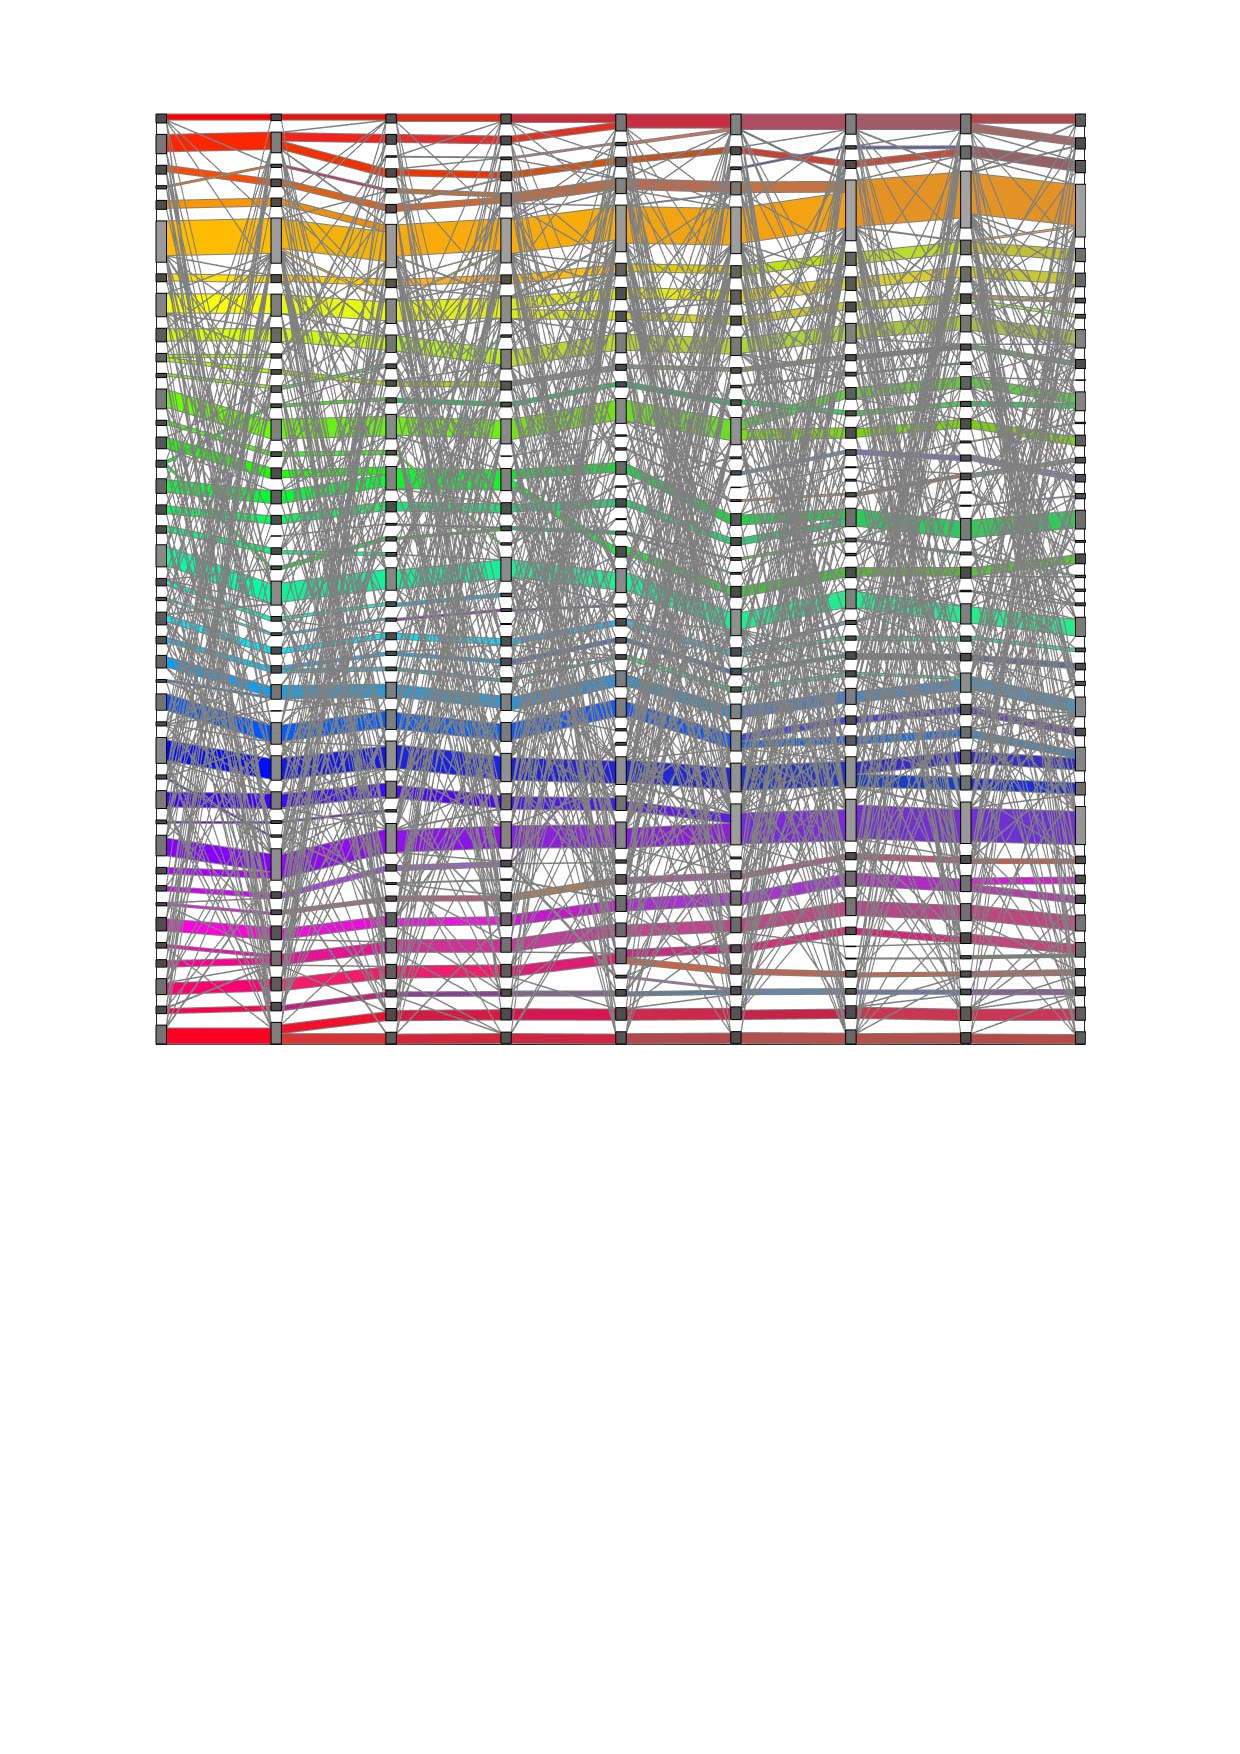
\includegraphics[width=.3\textwidth,height=.15\textwidth]{figures/chap03/dsbm/ASONEMmsEvolution/1HBDSBM.pdf}
	}
	\subfigure[GenLouvain]{
		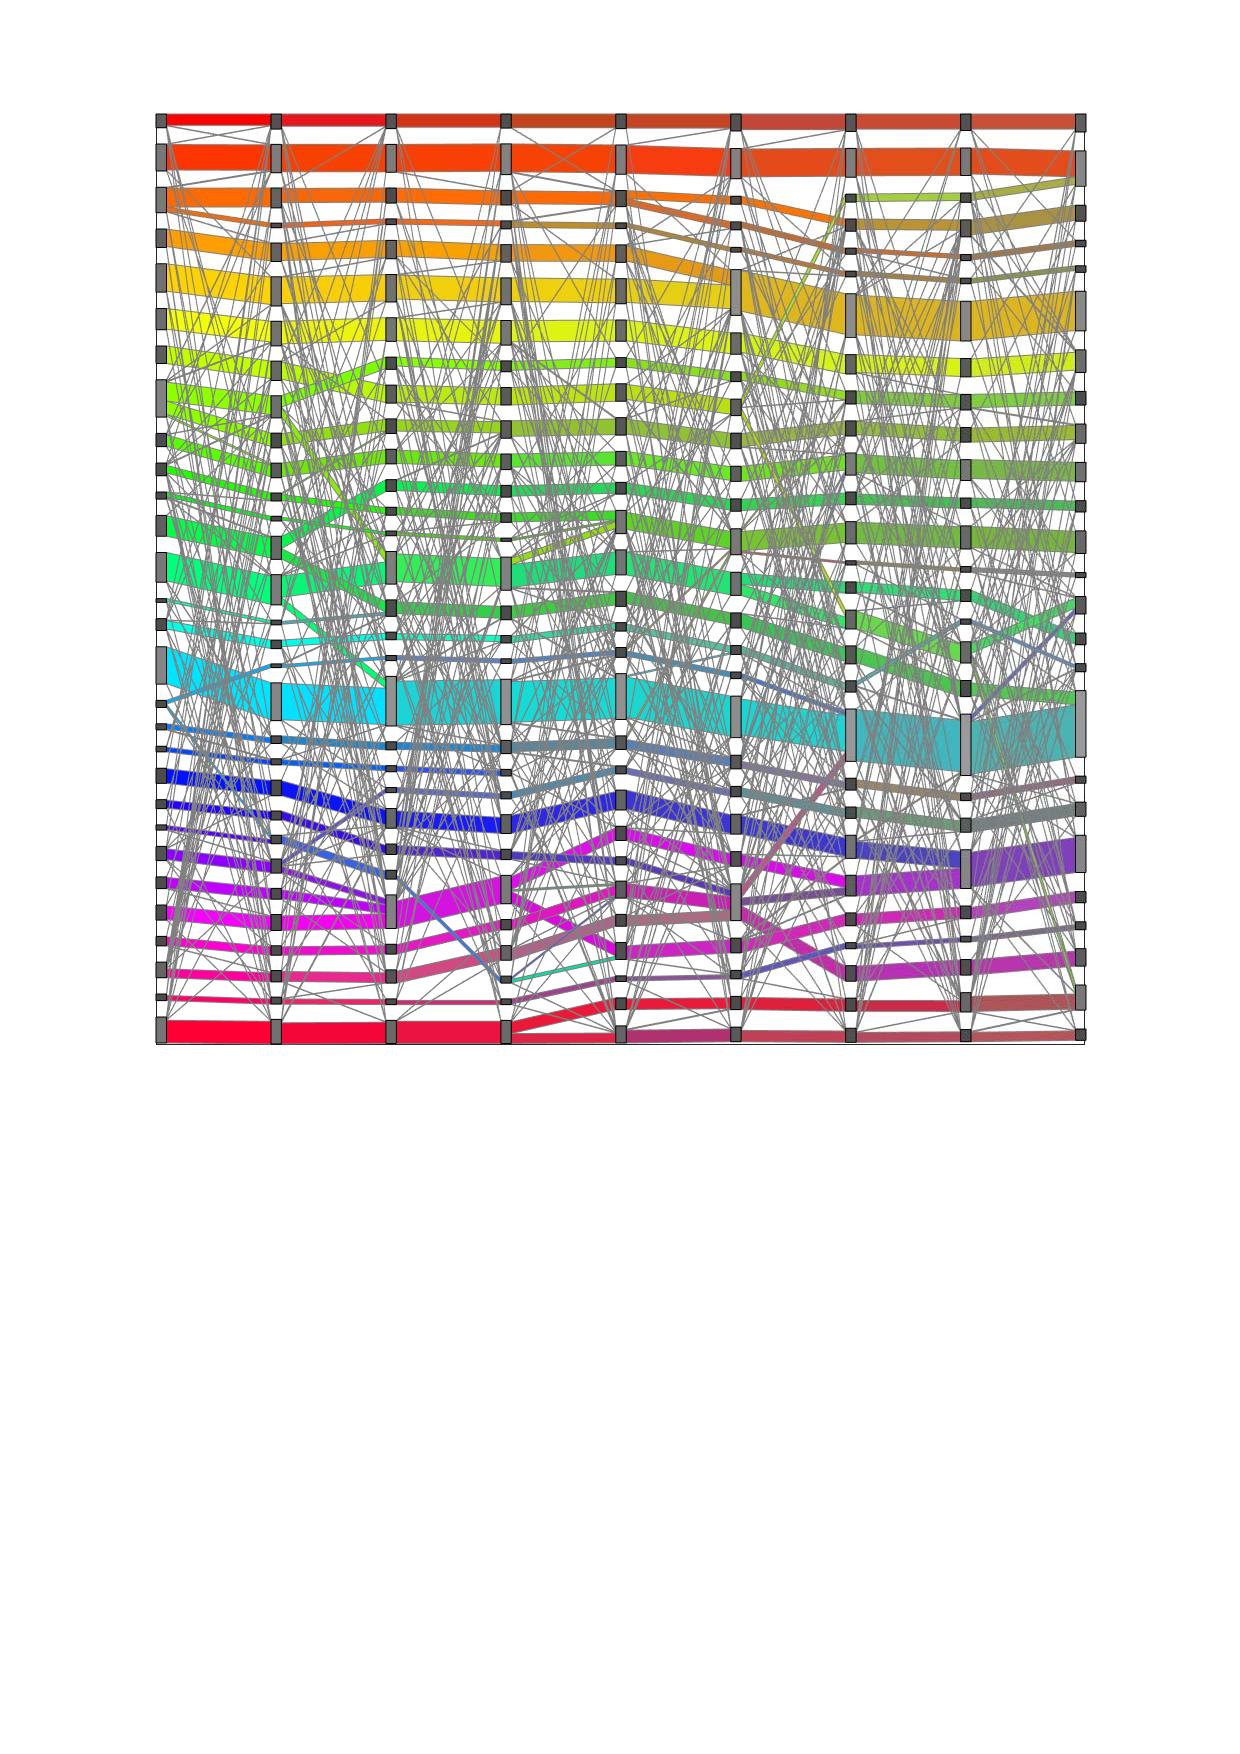
\includegraphics[width=.3\textwidth,height=.15\textwidth]{figures/chap03/dsbm/ASONEMmsEvolution/1gen.pdf}
	}
	\subfigure[PisCES]{
		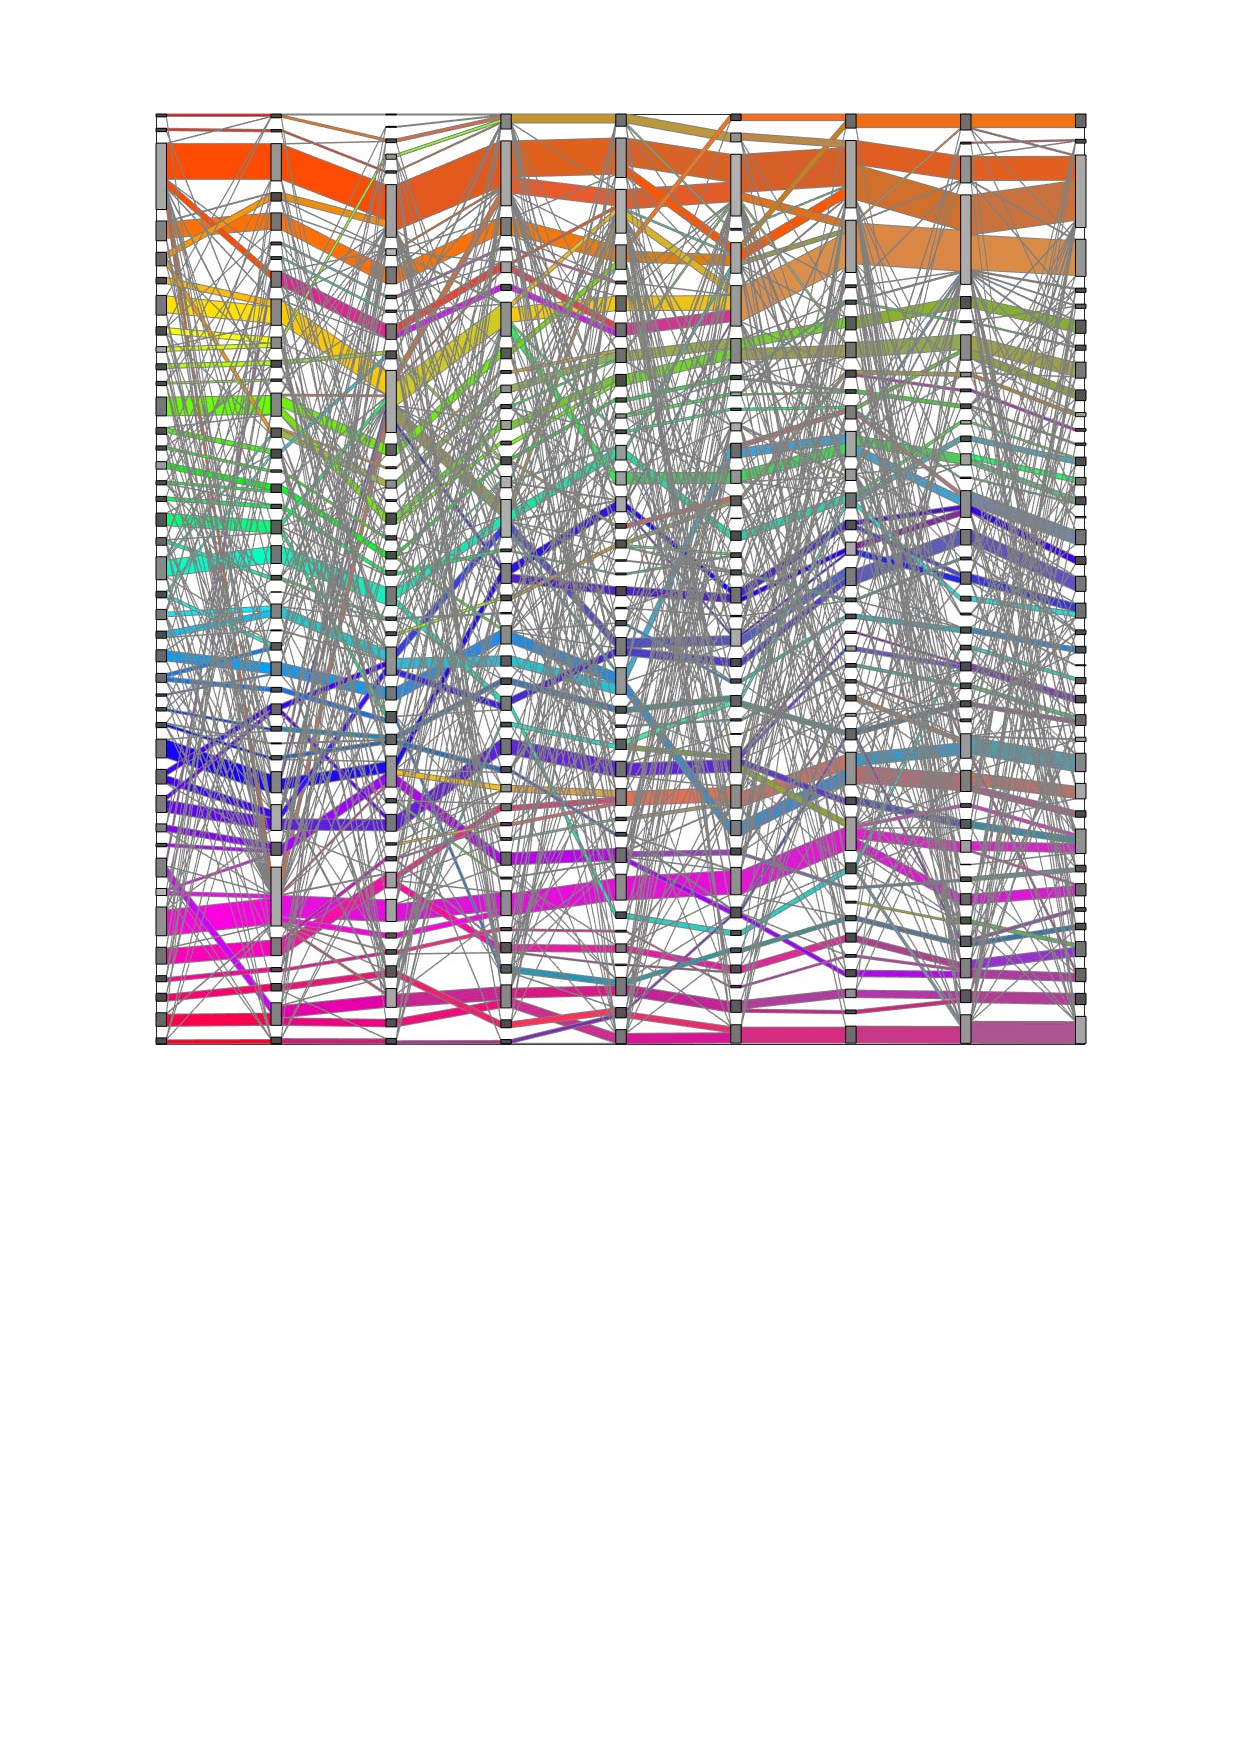
\includegraphics[width=.3\textwidth,height=.15\textwidth]{figures/chap03/dsbm/ASONEMmsEvolution/1PisCES.pdf}
	}
	\subfigure[DYNMOGA]{
		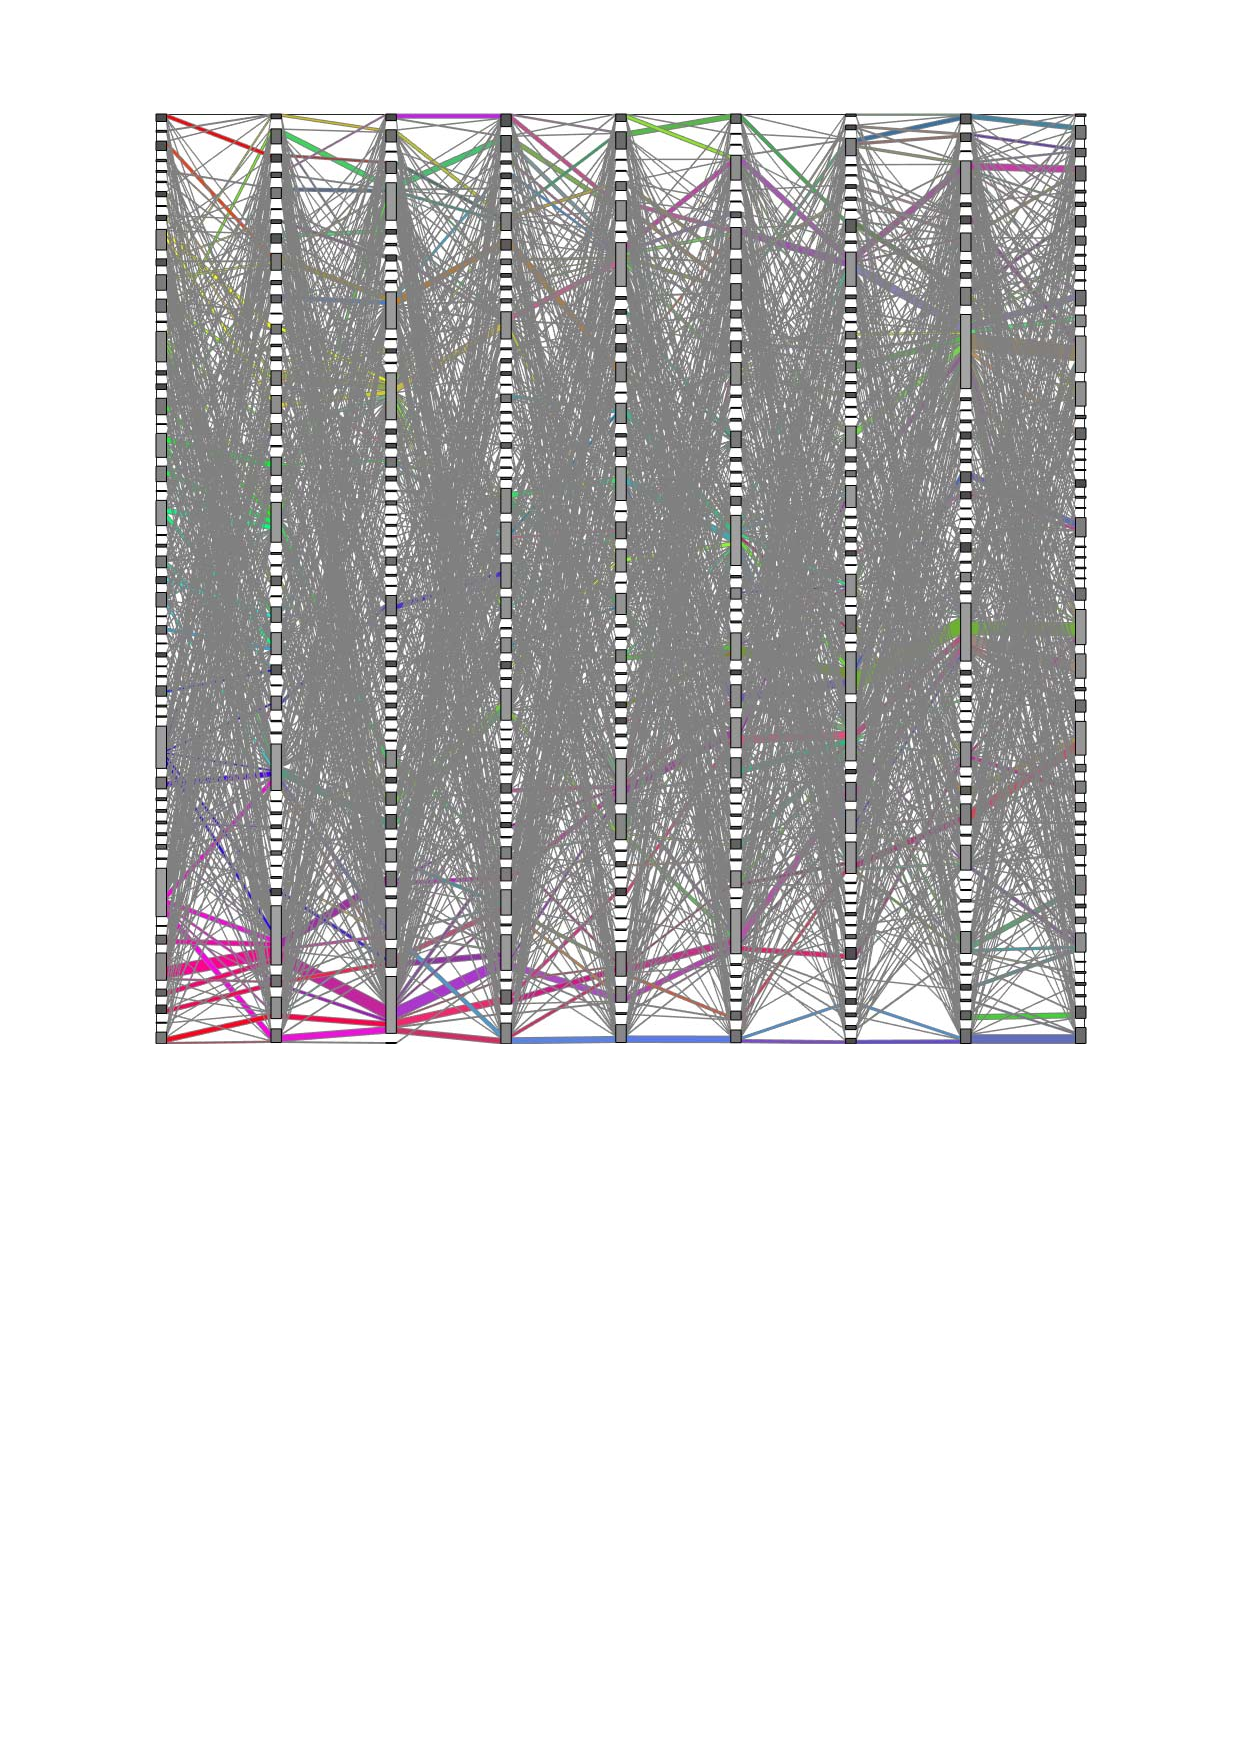
\includegraphics[width=.3\textwidth,height=.15\textwidth]{figures/chap03/dsbm/ASONEMmsEvolution/1dynmoga.pdf}
	}
	\caption{生成数据2中社团分裂合并事件数据的社团演化桑基图}
	\label{fig:SankeyAsonamMS}
	%  \vspace{-0.5cm}
\end{figure}

\begin{figure}
	\centering
	\subfigure[GroundTruth]{
		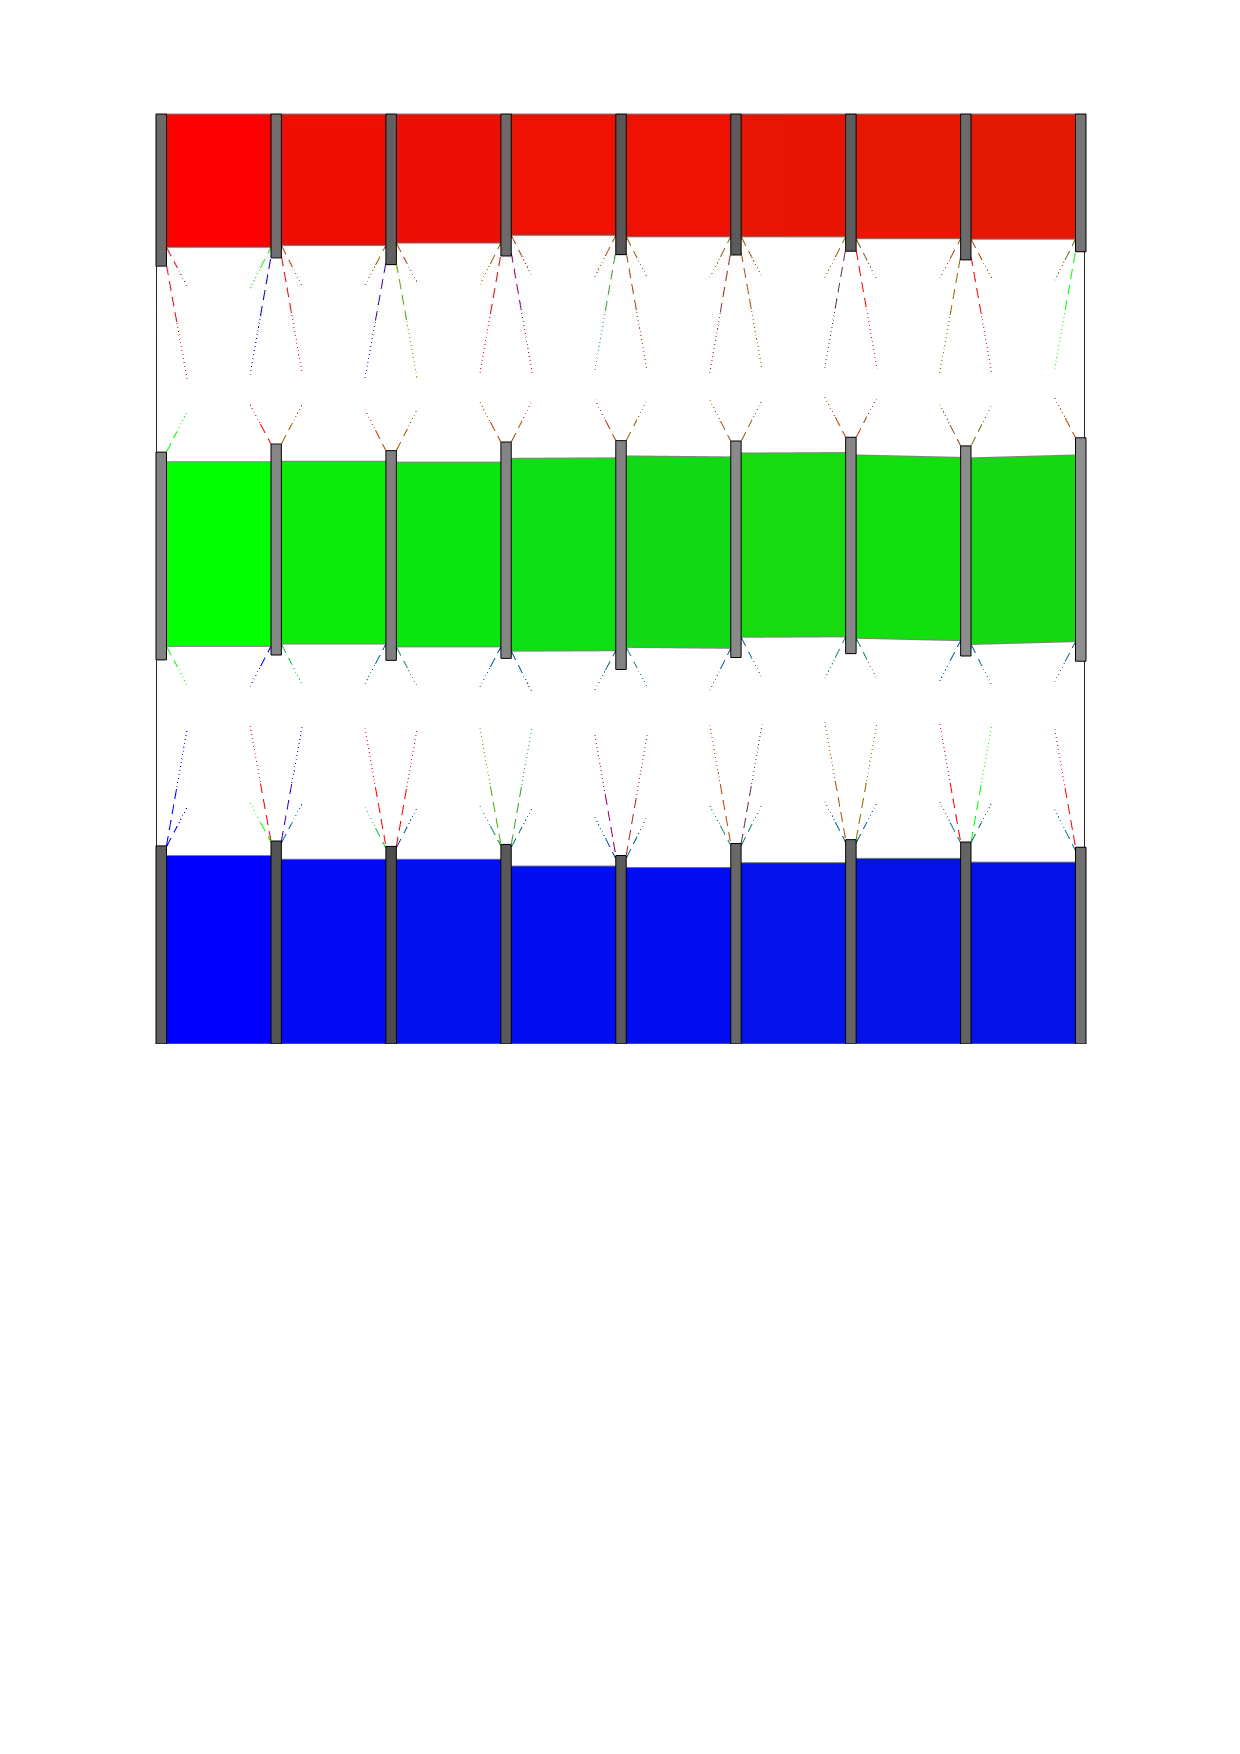
\includegraphics[width=.3\textwidth,height=.1\textwidth]{figures/chap03/dsbm/dblpEvolution/GroundTruth.pdf}
	}
	\subfigure[DSBM]{
		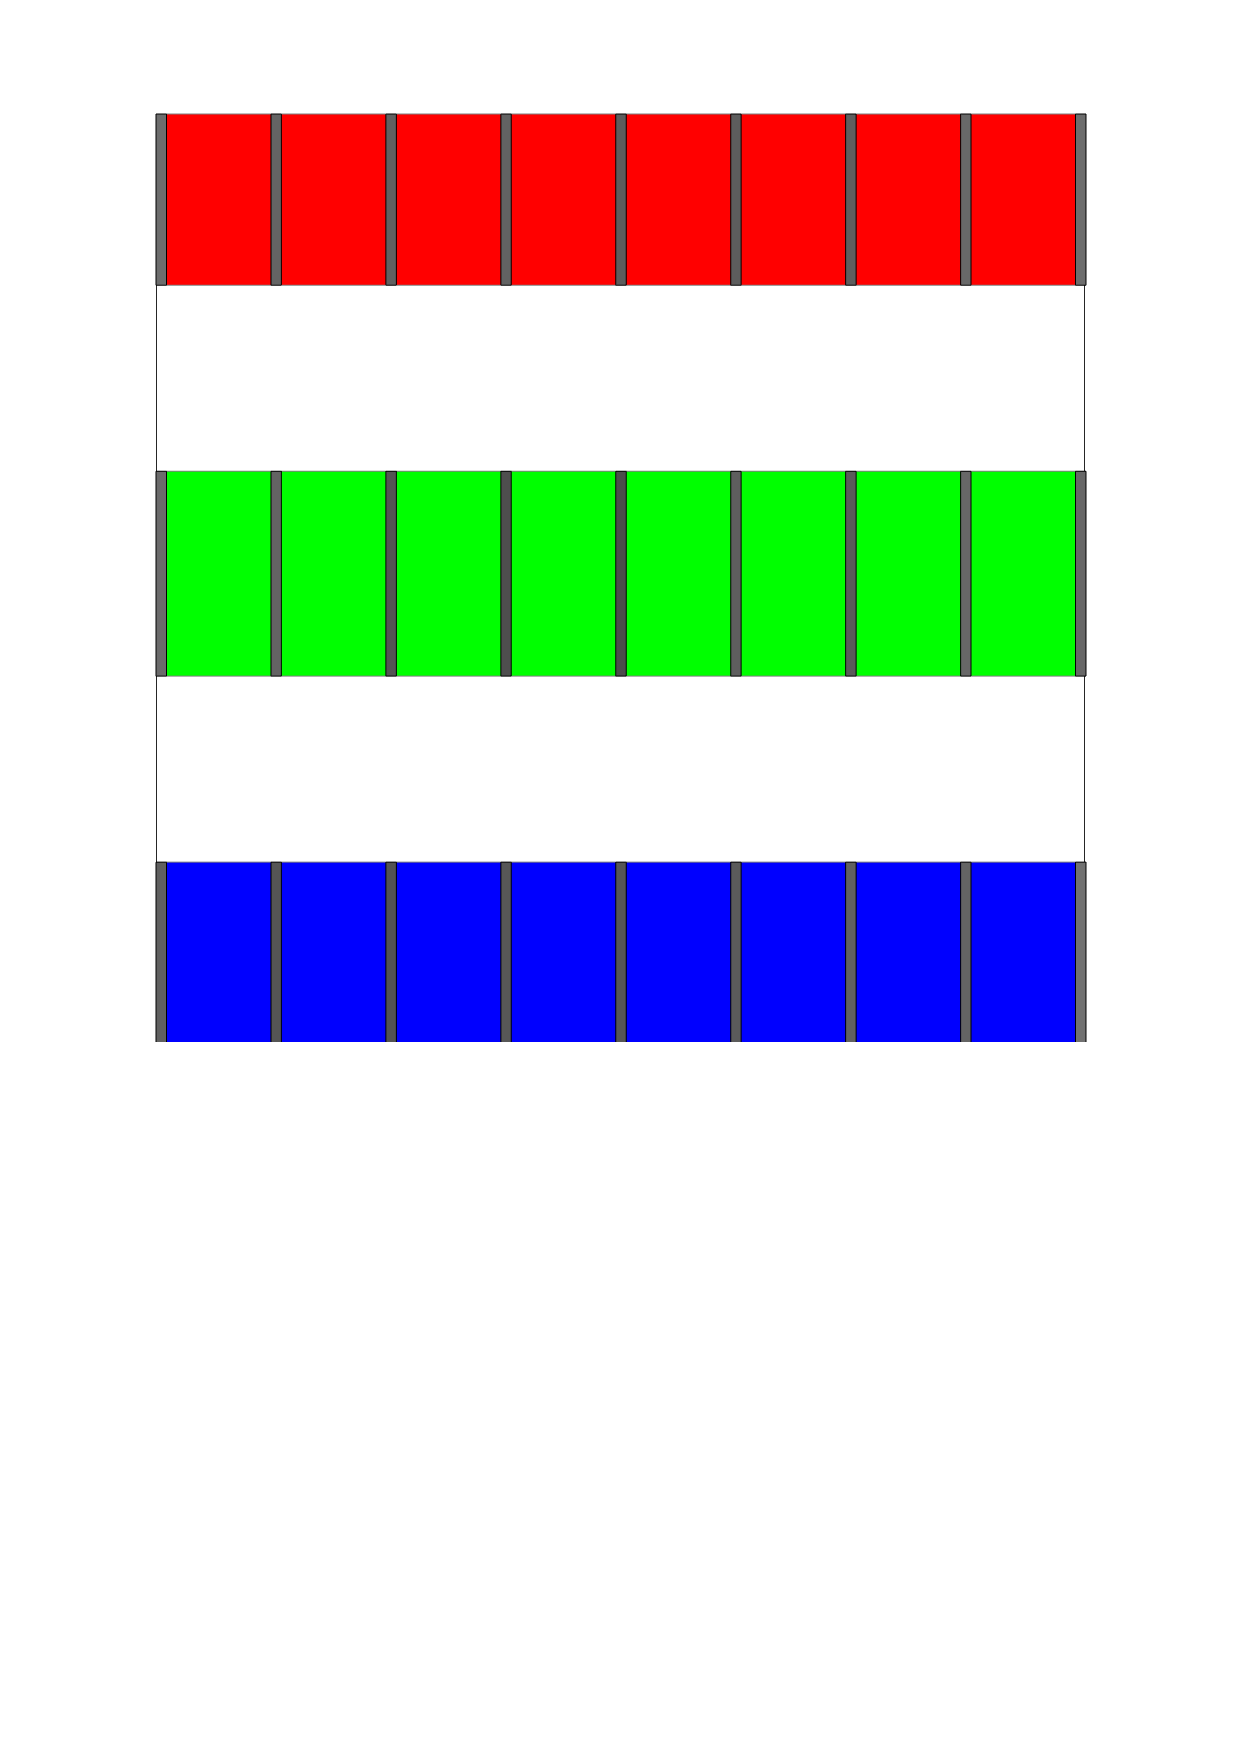
\includegraphics[width=.3\textwidth,height=.1\textwidth]{figures/chap03/dsbm/dblpEvolution/DSBM.pdf}
	}
	\subfigure[HB-DSBM]{
		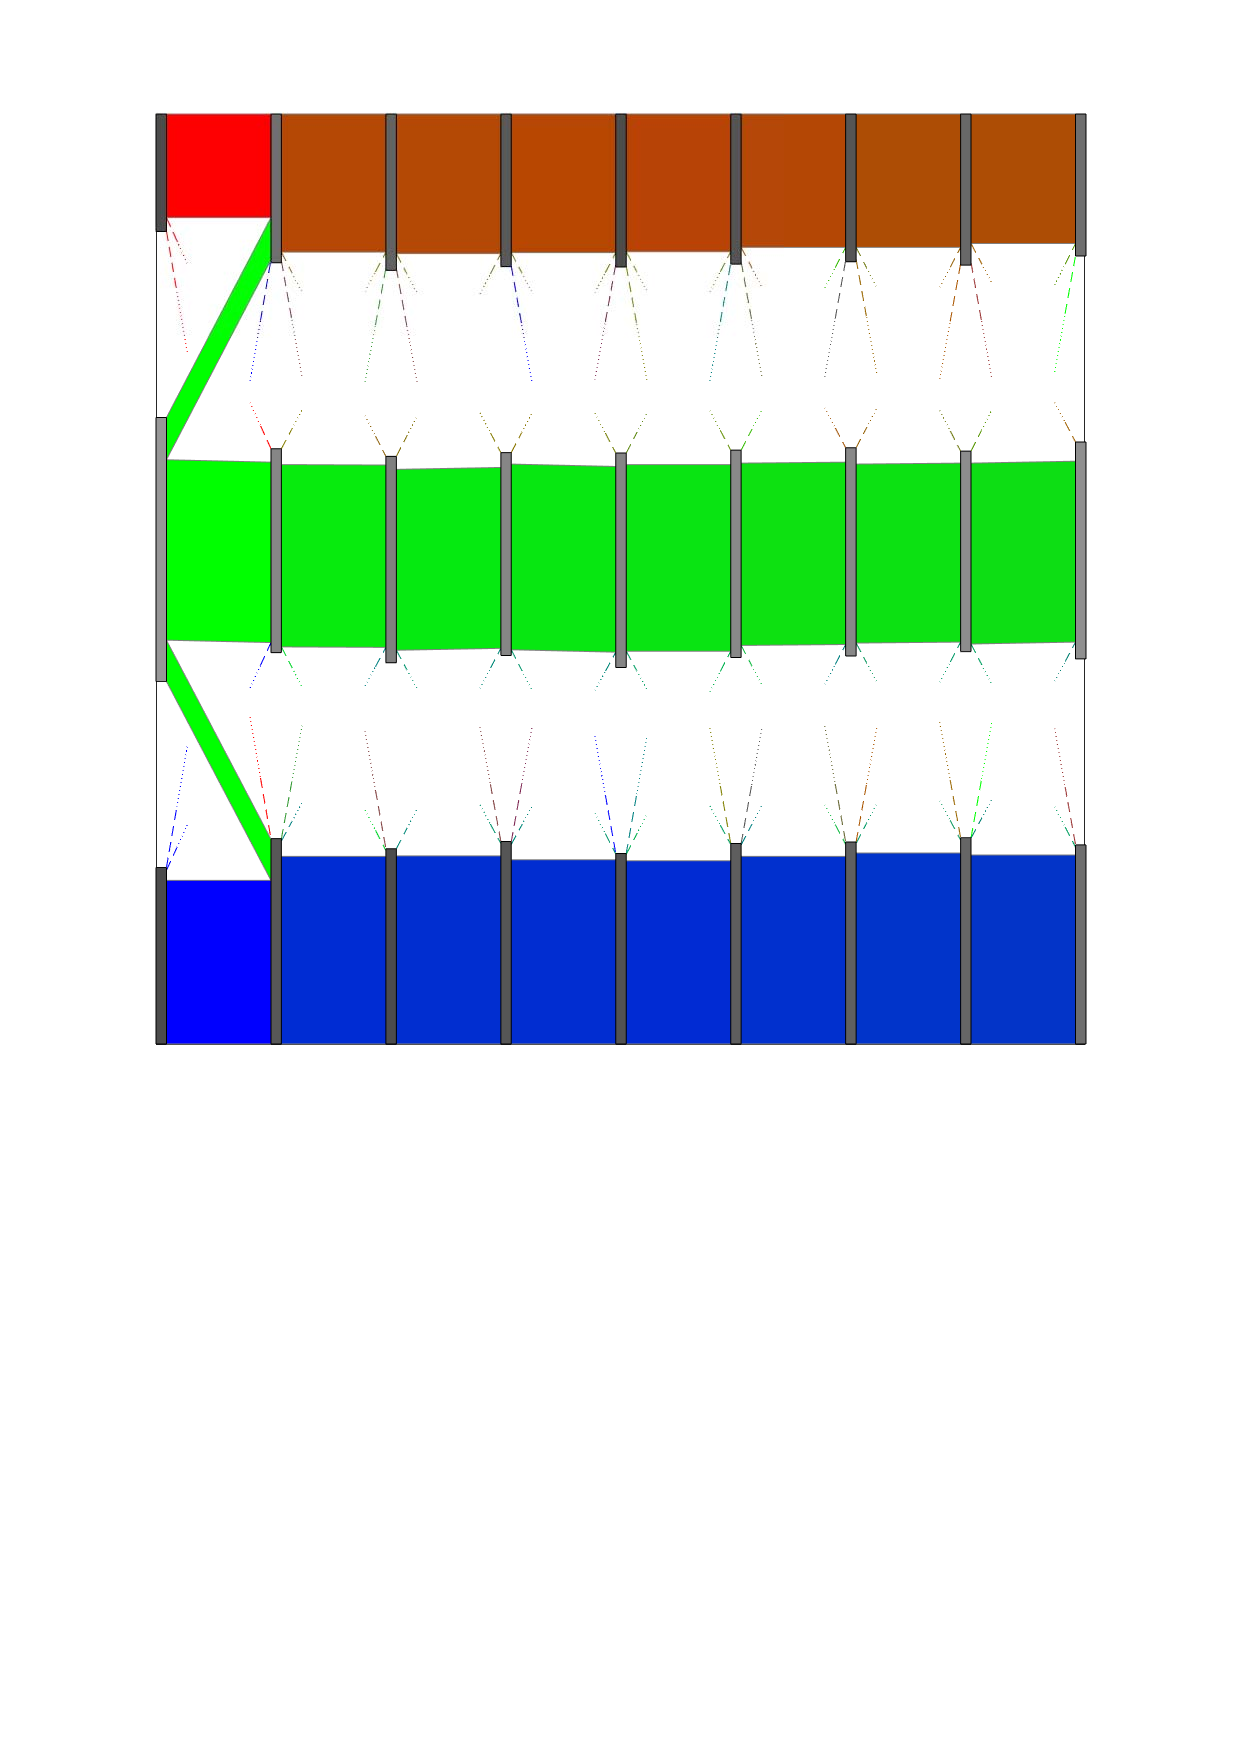
\includegraphics[width=.3\textwidth,height=.1\textwidth]{figures/chap03/dsbm/dblpEvolution/HB-DSBM.pdf}
	}
	\subfigure[GenLouvain]{
		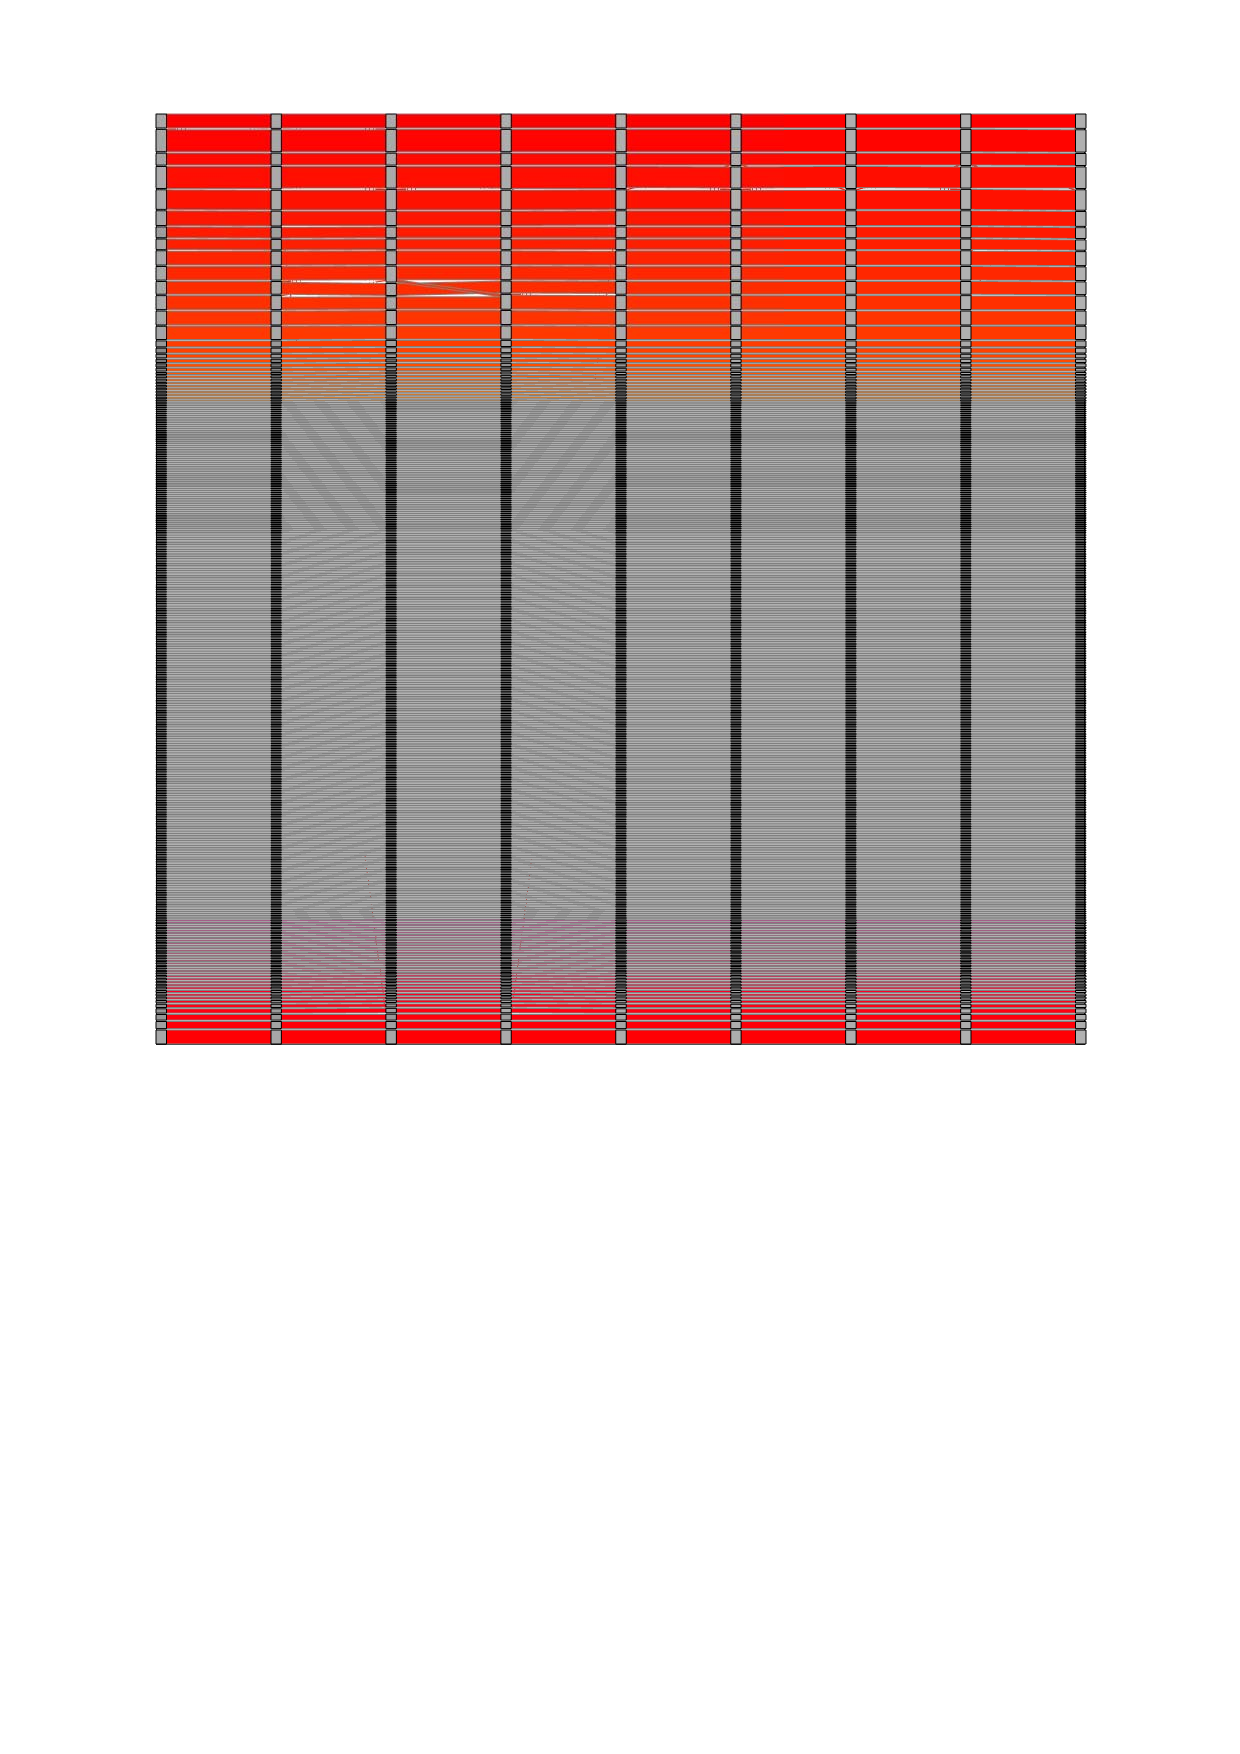
\includegraphics[width=.3\textwidth,height=.1\textwidth]{figures/chap03/dsbm/dblpEvolution/gen.pdf}
	}
	\subfigure[PisCES]{
		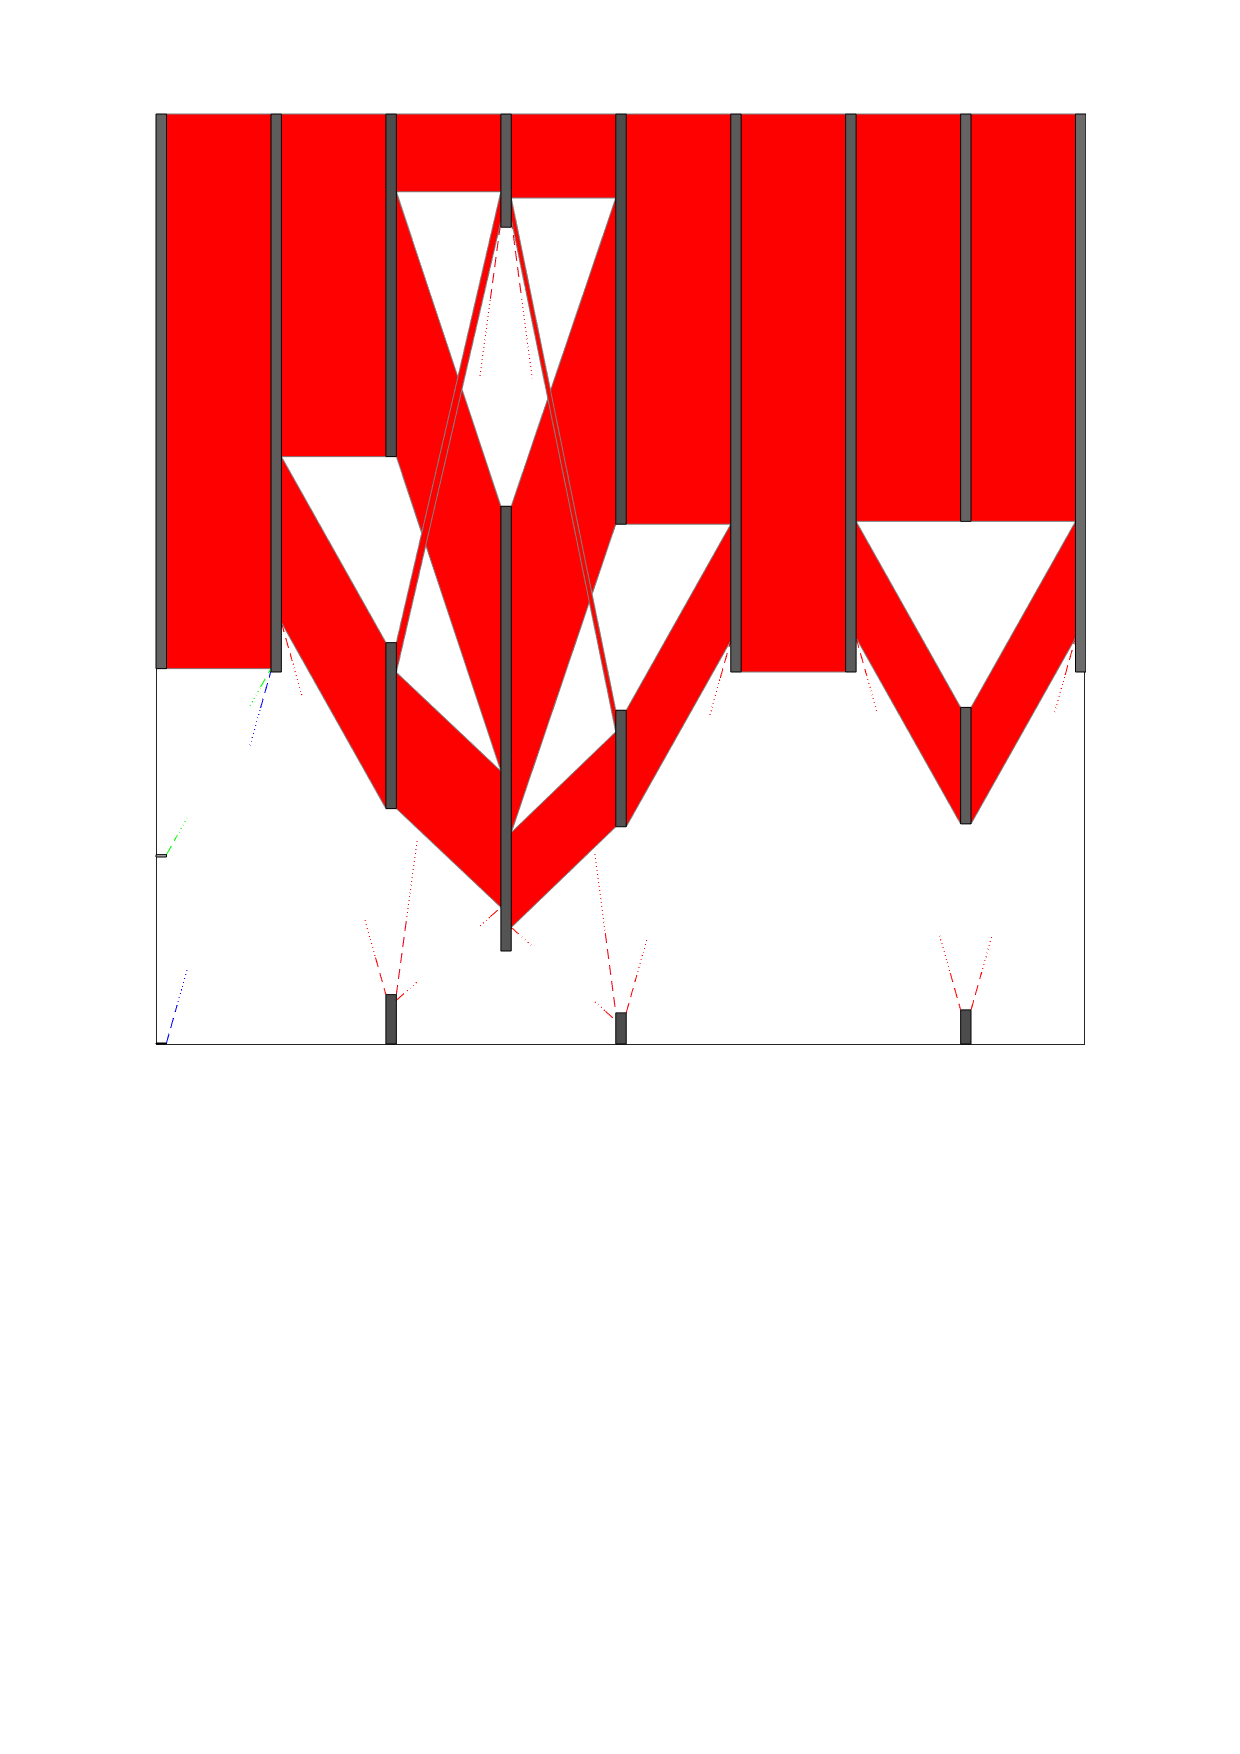
\includegraphics[width=.3\textwidth,height=.1\textwidth]{figures/chap03/dsbm/dblpEvolution/PisCES.pdf}
	}
	\subfigure[DYNMOGA]{
		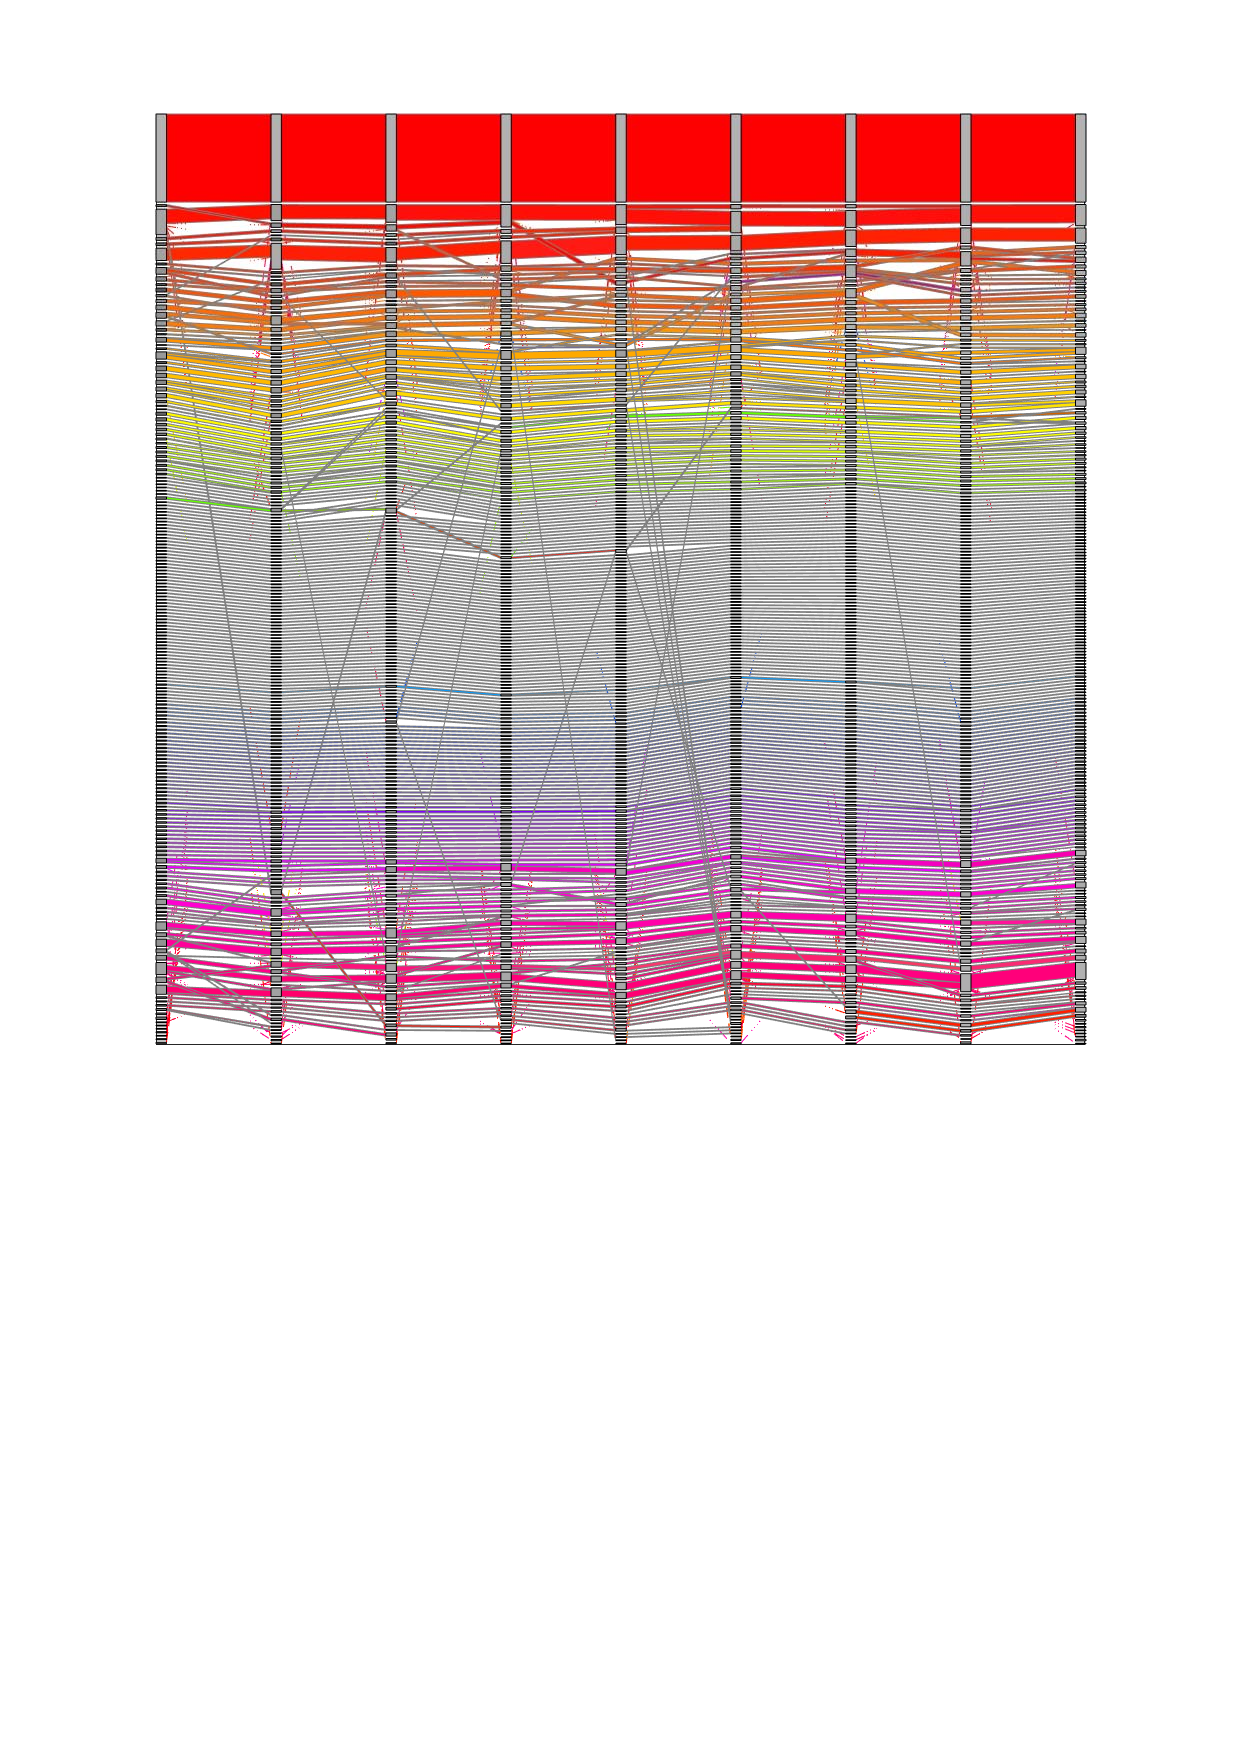
\includegraphics[width=.3\textwidth,height=.1\textwidth]{figures/chap03/dsbm/dblpEvolution/dynmoga.pdf}
	}
	\caption{DBLP数据的社团演化桑基图}
	\label{fig:SankeyDBLP}
	%  \vspace{-0.5cm}
\end{figure}

另外,本节还分析了HB-DSBM的社团转移矩阵$A$的实际意义,如图~\ref{fig:block}所示,热图中颜色越浅表示转移倾向越高。可以看到HB-DSBM的社团转移矩阵符合社团的定义,同时所建模的节点转移异质性也起到了有效作用,节点更倾向于在时序过程中保留在本社团内,但保留了转移到其他社团的倾向,而DSBM则更加极端。PisCES对社团转移的倾向刻画则更加混乱。



\begin{figure}
\centering
\subfigure[DBLP]{
	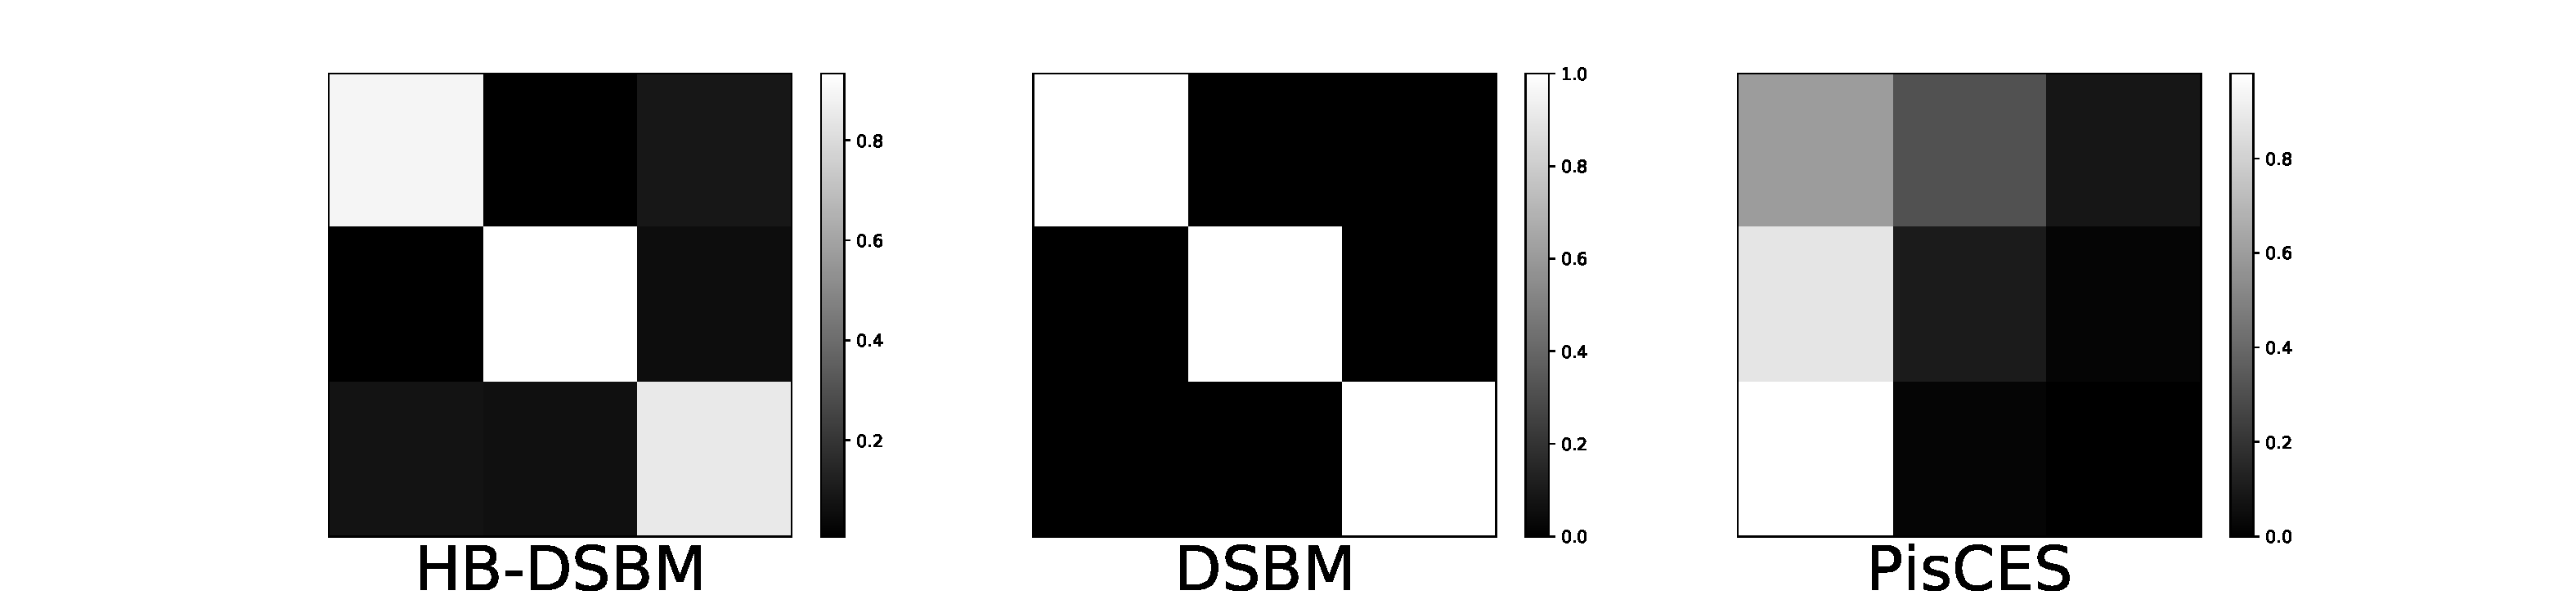
\includegraphics[width=.46\textwidth]{figures/chap03/dsbm/blockMatrixVis/dblpcommunityHeatMap3.pdf}
}
\;\;\;\;
\subfigure[生成数据$2$分裂合并数据]{
	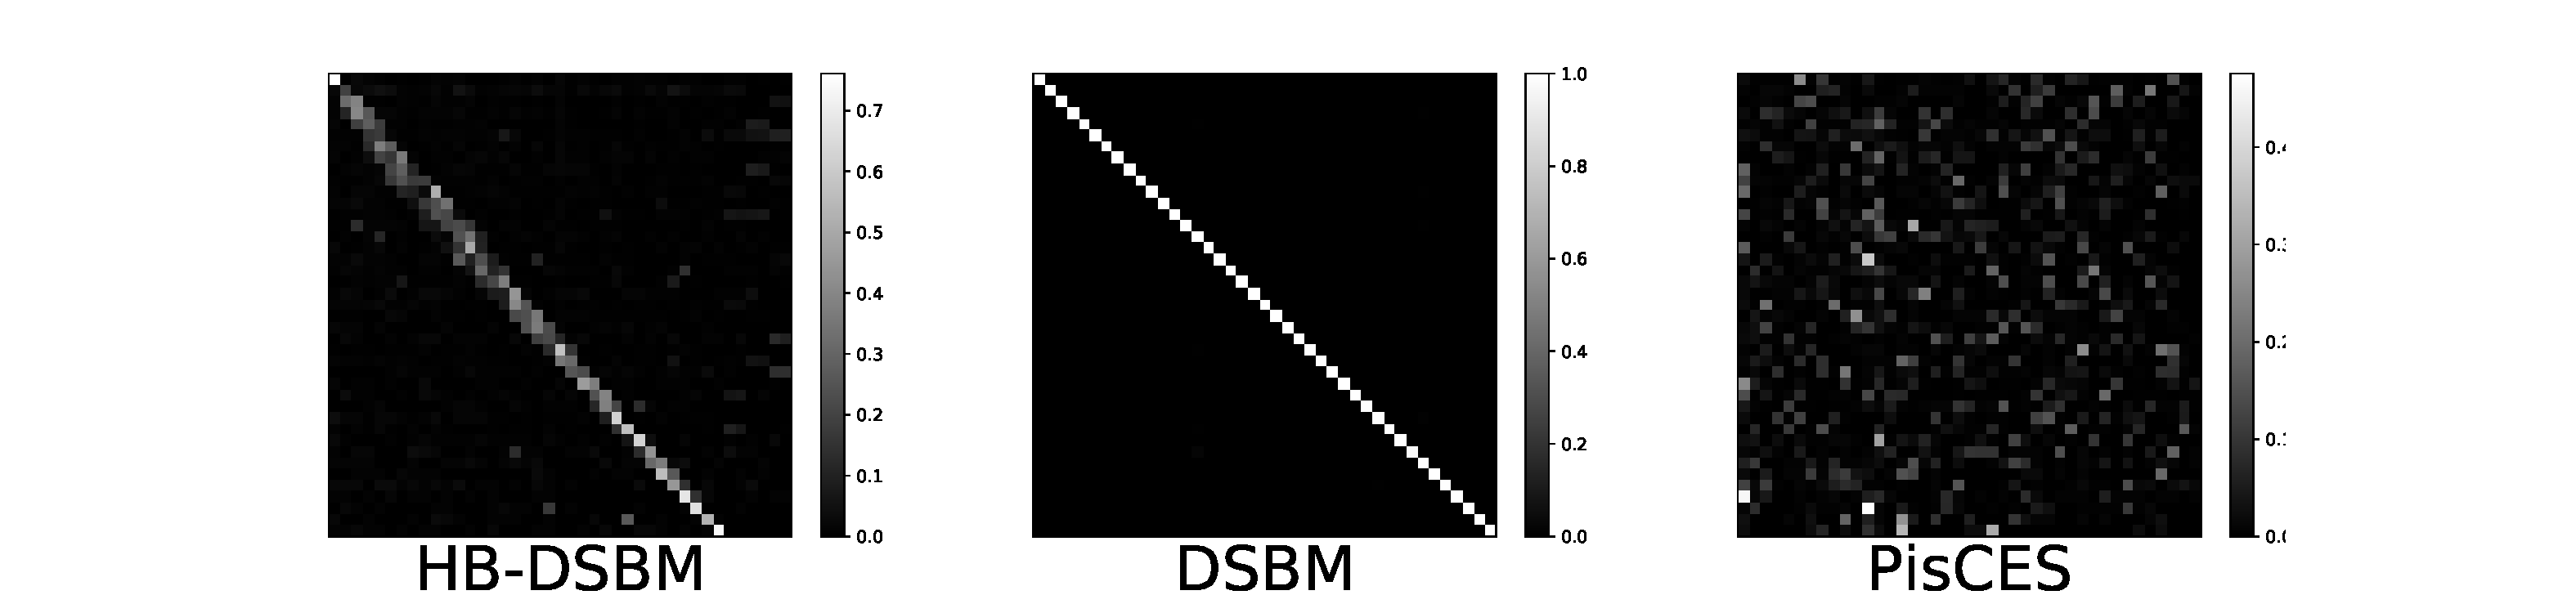
\includegraphics[width=.46\textwidth]{figures/chap03/dsbm/blockMatrixVis/ASONMScommunityHeatMap3.pdf}
}
% \subfigure[FacetNet $\sigma = 5$, $nC = 9$, and $aD = 20$ ]{
	% 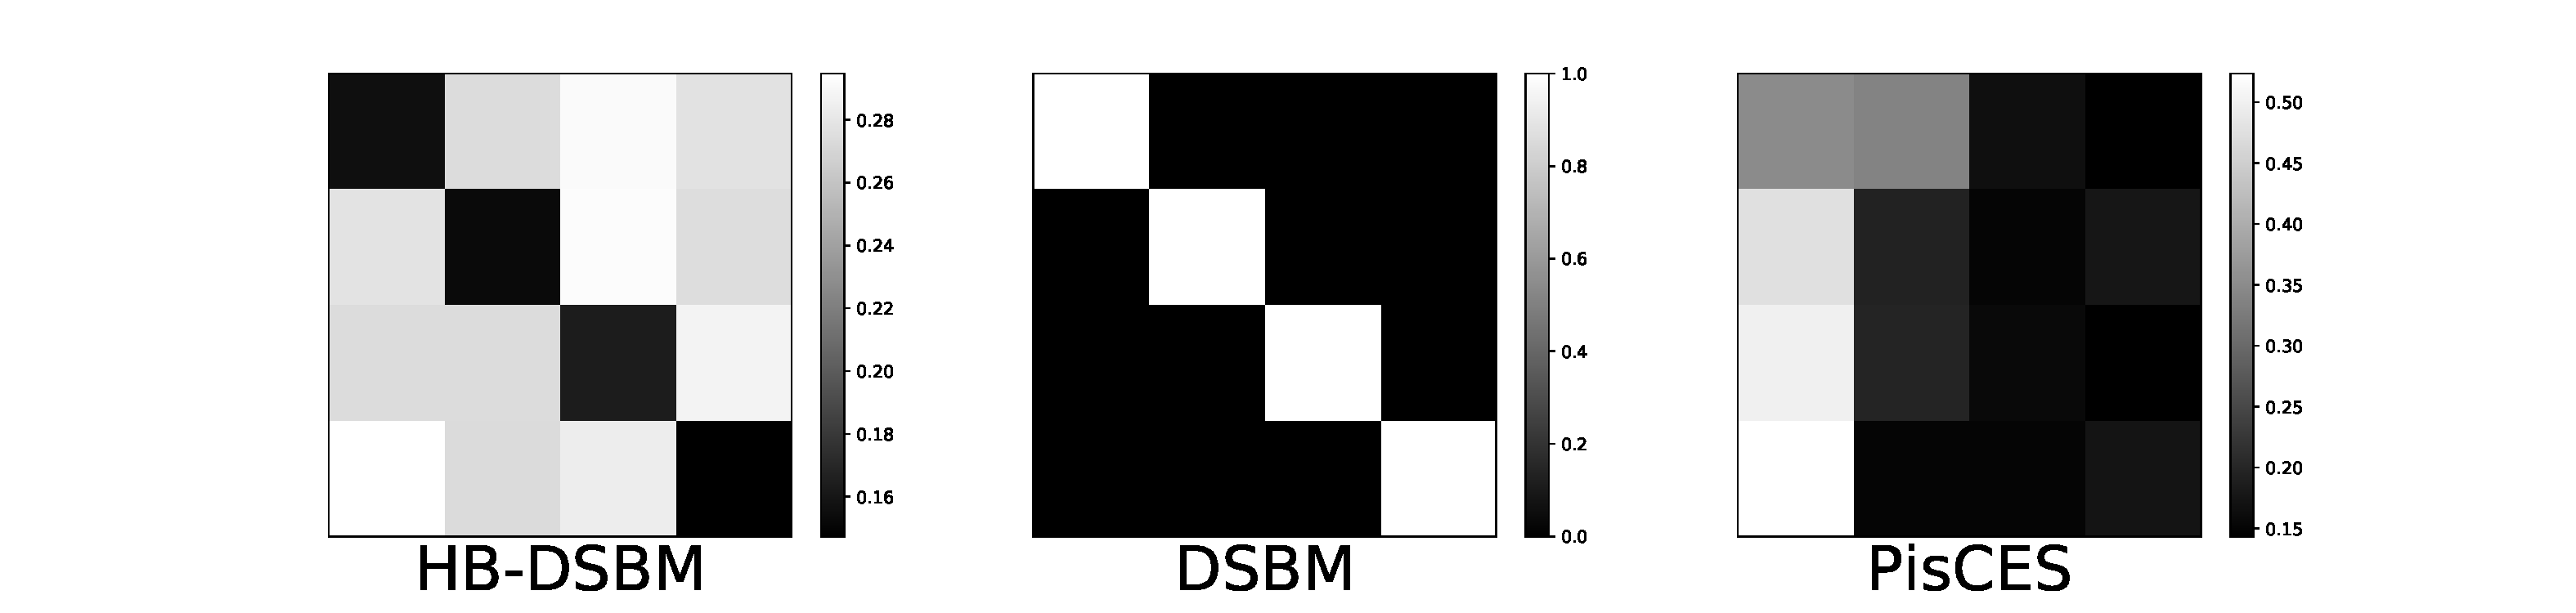
\includegraphics[width=.48\textwidth]{pictures/blockMatrixVis/facetNet5920communityHeatMap3.pdf}
	% }
\caption{社团转移矩阵$A$的热图可视化}% Notice that only DSBM, HB-DSBM and PisCES have `block matrix'. }
\label{fig:block}
%\vspace{-0.5cm}
\end{figure}

\subsection{节点的演化异常分析}
另外,为了验证节点及转移参数$C$的实际意义与有效性,本章根据$C$对节点演化异质性的概念,提出了节点演化异常的定义,即在动态网络中存在频繁变换其社团归属的节点,并利用熵对节点$i$的演化异常指数进行定义:
\begin{equation}
	E_i = -\sum_{t=1}^{T-1} \sum_{k} C_{tik} \log C_{(t+1)ik},
	\label{Nodeanomaly3}
\end{equation}
$E_i$越大,表示节点$i$的演化越频繁,则认为其是异常节点。如图~\ref{fig:anomalyPics}所示,在DBLP数据中,$E_i$较高的节点较少,整体呈现出较稳定的趋势,证明DBLP数据中,研究人员的研究领域相对稳定,这由图~\ref{fig:SankeyDBLP}可以进行佐证。而专利数据Patent则呈现出了剧烈的节点变动,证明在计算机领域的专利合作并不像论文合作一样稳定,从直观上来看,专利的发表更关注第一发明人,其余发明人的权重在我国并不高,这也验证了该结论。而针对生成数据2中社团分裂合并数据的测试则验证了所定义的节点异常指数的有效性。


\begin{figure}
	\centering
	\subfigure[DBLP]{
		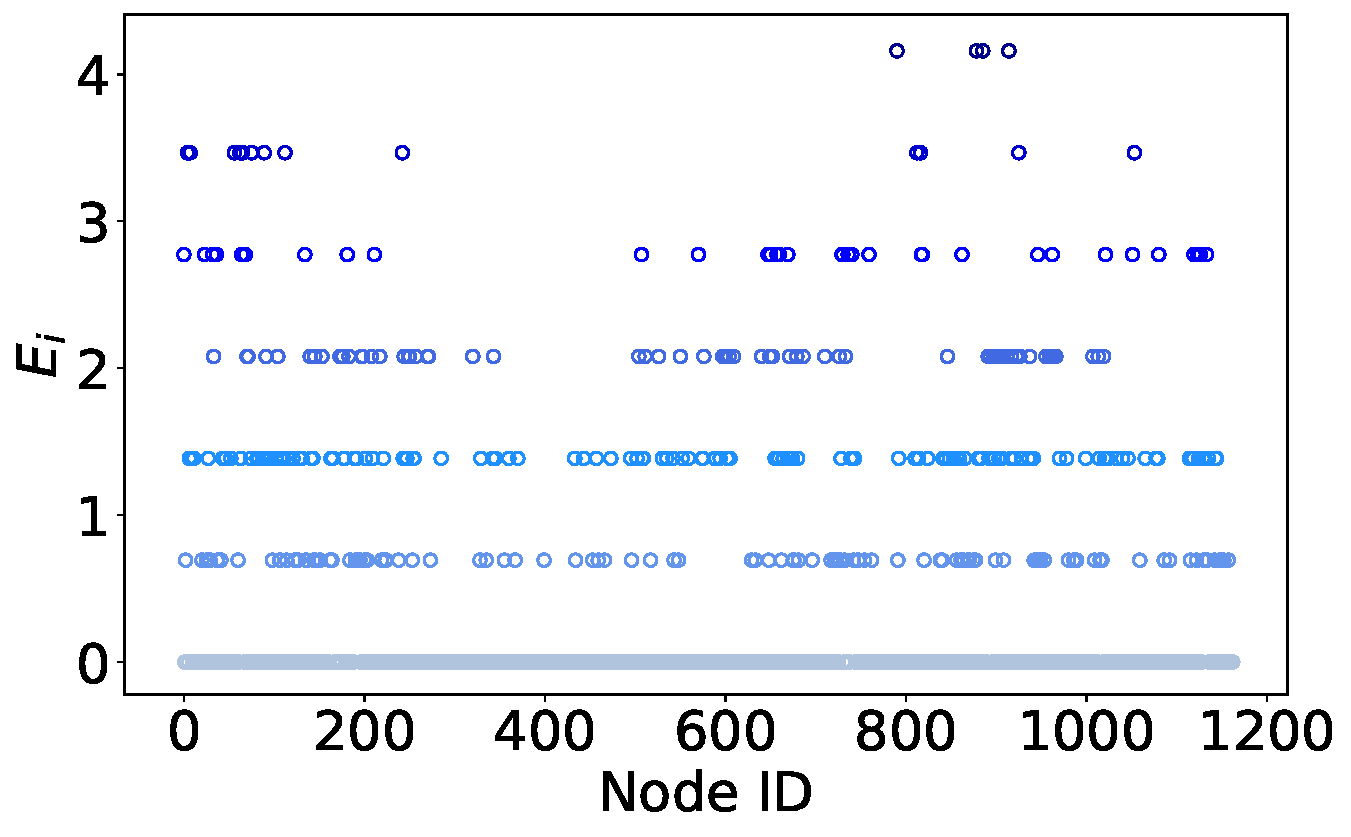
\includegraphics[width=.3\textwidth]{figures/chap03/dsbm/anomaly/dblpAnomalyPic6.pdf}
	}
	\subfigure[Patent]{
		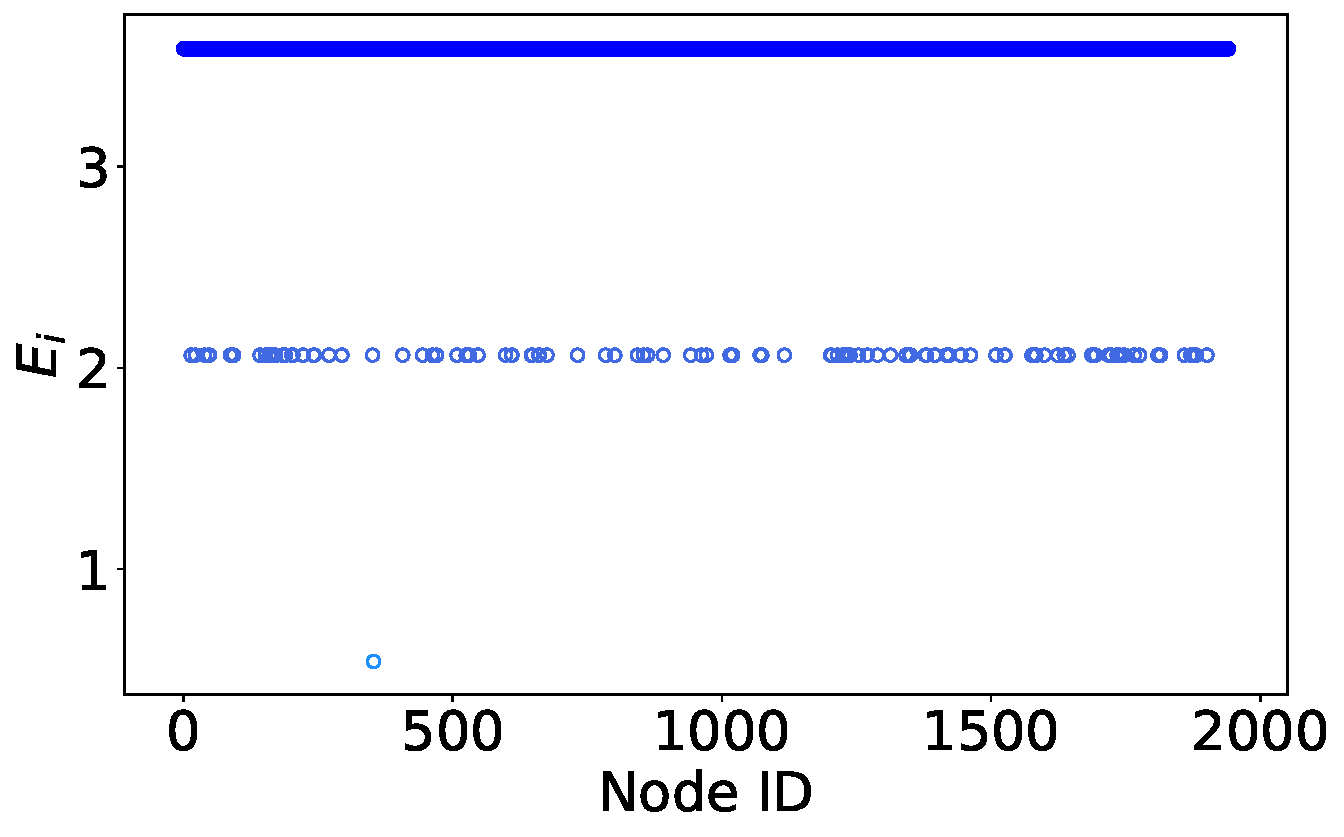
\includegraphics[width=.3\textwidth]{figures/chap03/dsbm/anomaly/patentAnomalyPic6.pdf}
	}
	\subfigure[生成数据2分裂合并数据]{
		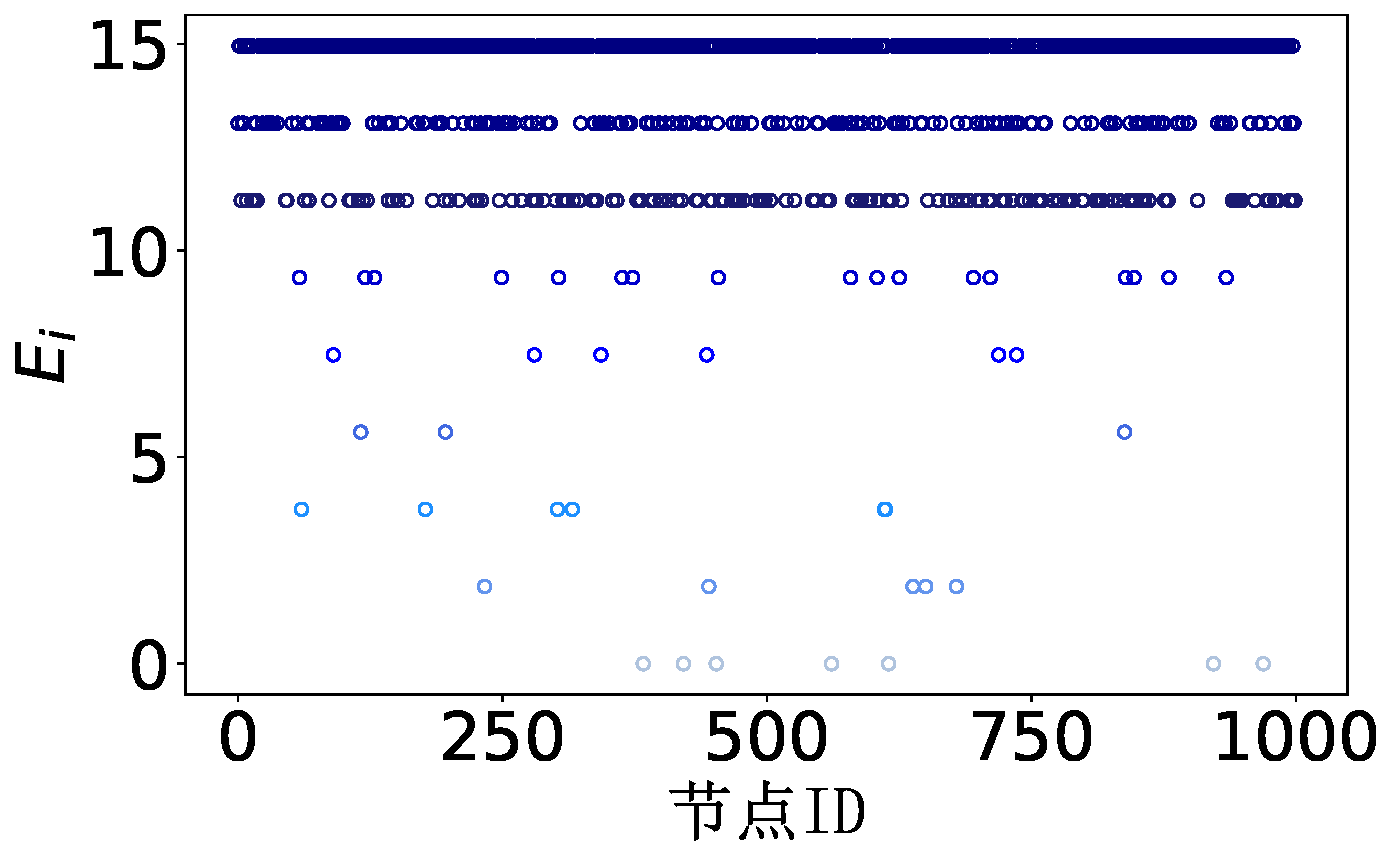
\includegraphics[width=.3\textwidth]{figures/chap03/dsbm/anomaly/msAnomalyPic6.pdf}
	} 
	\caption{基于节点级转移参数$C$的节点演化异常点可视化图}
	\label{fig:anomalyPics}
	%   \vspace{-0.5cm}
\end{figure}


\section{本章小结}
本章首先从实际出发,通过创新性地将节点在动态网络的社团转移倾向异质性挖掘问题转化为节点的社团转移与否的二分类问题,对$15$个各类真实世界动态网络数据进行了实证分析,进而得出结论,\textbf{动态网络中,节点的社团转移存在异质性,且与节点的度具有较高关联性}。根据上述结论,本章进一步基于动态随机块模型设计了层次贝叶斯动态随机块模型,其层次贝叶斯生成结构能够在刻画动态社团演化模式时同时建模节点的社团转移异质性。另外针对所提出的HB-DSBM模型,利用变分推断对模型参数的更新进行了详细的推断,利用合理的优化策略,模型具备适应大规模数据计算的潜力。同类方法的对比也显示出HB-DSBM在动态网络社团检测以及社团演化分析任务中更加高效准确。另外,本文提出的基于节点转移异质性参数提出的节点演化异常指数也在实际分析中得以验证其有效性。

然而从模型设计的角度来看,HB-DSBM仍然存在一定缺陷,首先,其对节点的社团转移异质性建模主要从生成角度而进行的设计,即假设节点的社团转移异质性与社团级别的节点转移倾向有关。具体来说,节点的社团转移异质性服从以其社团级别社团转移倾向为参数的狄利克雷分布。该设计虽然合理,但该参数并未与动态网络中的节点属性直接关联,因此在实际的下游任务中无法直接用于解释不通节点的社团转移倾向;其次,生成模型的优势之一是对于多种下游任务的适配,而所提出的节点演化异常指数还有进一步挖掘其能力的可能。因此,后续章节将针对HB-DSBM中存在的上述问题进行改进。












% % !Mode:: "TeX:UTF-8"
% \baselineskip 20pt

% %\chapter{个性化显著性评估驱动的评论摘要生成}
% \chapter{基于贝叶斯模型的动态网络层次演化建模(考虑异质性)}
% \label{chap4}
% 上一章介绍了基于决策树的社团转移因素探究框架,通过$15$个真实数据集的分析得到了影响节点社团转移的两个节点的结构属性:节点的度和节点的平均邻居度。受上一章启发,本章认为每个节点的社团转移由于其局部结构不同,都具有不同的转移倾向。而现有的动态网络社团检测模型大部分都将主要的关注点投入到了每个时间快照的社团检测上,而忽略了社团演化,小部分方法如DSBM~\cite{yang2011detecting}虽然关注了社团演化,但是其仅仅通过社团转移矩阵$A$来刻画社团级别的演化,而忽略了同一个社团内的每个节点的社团转移倾向的异质性,也就是说,在DSBM中,其假设同一个社团内的节点在下一个时刻发生转移的趋势都是一样的,且这种趋势在某个固定的社团内是一直不变的。这种假设在本文看来是不合理的。因此本章将会介绍引入更细粒度社团转移趋势的动态网络社团检测生成模型HB-DSBM。
% \section{引言}

% 基于概率模型的社团检测方法,尤其是基于随机块模型(SBM)的方法在动态网络社团检测中具有独特的地位。概率模型通过建立动态复杂网络的生成机制,将社团检测问题转化成了模型的参数估计问题,利用数据拟合模型参数,从而构建出完整的概率模型。利用这种方法进行动态网络社团检测的优点是,模型的任何参数都是可解释的,因此模型中的社团的形成机制也是可以解释的,这就使得人们可以通过概率模型对网络以及社团的生成以及演变过程具有更深层次的理解。而基于随机块模型的社团检测算法就是基于概率模型进行社团检测的算法中的重要一类算法。随机块模型最初的提出是用来解决静态网络社团检测问题,其具有三个基本假设:
% \begin{itemize}
% 	\item 网络中的社团个数是固定的;
% 	\item 每个节点只属于一个社团,且节点之间属于哪个社团是相互独立同分布的;
% 	\item 网络中的两个节点之间有边的概率只与其所在的社团有关。
% \end{itemize}
% 这些假设将网络的生成与社团相结合,从而使得利用生成模型进行社团检测成为可能。而在$2011$年,有人改进了随机块模型,引入了社团演化矩阵,将随机块模型扩展为动态随机块模型(DSBM)。动态随机块模型在动态社团检测中也具有不俗的效果,但是依然存在很多不合理的地方,限制了其社团检测结果。如社团个数固定的假设等,也有很多人对DSBM进行了改进,但是鲜有人注意到DSBM关于社团演化假设的不合理性。DSBM假设了节点的社团转移在所有时间片都是一致的,且只与所在社团有关,这显然是不合理的。本文即在此提出了层次贝叶斯结构重新刻画了节点的社团转移倾向概率。

% 受上一章的启发,本章假设动态网络中同一个社团的不同节点在社团转移行为上具有不同的倾向性,这是由不同节点在社团内具有不同的局部结构决定的。因此本文构建了生成模型HB-DSBM,引入了节点的社团转移倾向参数$C$来刻画每个节点的社团转移倾向。HB-DSBM根据概率图模型对动态网络进行建模,其特点是可以通过对网络的生成机制以及社团的产生机制进行推断并建模,将社团检测这一聚类问题转化为了模型的参数估计问题。而缺点是由于模型较复杂,传统的采样方法较慢,并不能适应大规模数据集,因此本章对HB-DSBM的求解使用了变分推断的方法,结合随机采样能够大大提高模型参数估计的效率。

% \section{HB-DSBM模型构建}

% \subsection{符号表示}
% \begin{table}
% 	\centering
% 	\caption{HB-DSBM模型的符号表示}\label{tab.4.1}
% 	\begin{tabular}{cc}
% 		\hline
% 		{\bfseries 符号} &  { \bfseries 描述} \\
% 		\hline
% 		$K$,$N$,$T$ & 分别为社团个数、节点数和时间快照数 \\
% 		\hline
% 		$W^{t}$ & $t$时间快照对应的邻接矩阵\\
% 		\hline
% 		$\pi_k$ & 在时间快照$1$中,$i$节点属于社团$k$的概率\\
% 		$z_i^{t}$ & 在$t$快照中,$i$节点属于哪个社团 \\
% 		${A}_k$ & $k$社团的社团级别转移倾向 \\
% 		${C}_i^{t}$ & $i$节点在$t$快照中的节点级别转移倾向, 其中$t=2, \cdots, T$,$i=1, \cdots, N$\\
% 		$B_{kl}$ & 属于$k$社团的节点与属于$l$社团的节点在任意时间快照中的连边概率\\
% 		\hline
% 		${\gamma}$ ,${\mu}$ & ${\pi}$和${A}_k$的狄利克雷分布参数 \\
% 		${\alpha}$ , ${\beta}$ & $B$的Beta分布的参数 \\   
% 		\hline
% 	\end{tabular}
% \end{table}

% 在介绍模型前,本章首先介绍模型的符号表示。如表\ref{tab.4.1}所示,本章用$W=\{W^1,W^2,...,W^T\}$表示动态网络邻接矩阵,即$W^t$表示第$t$个网络快照的邻接矩阵,其中$t \in 1,...,T$。这里$W^t \in \{0,1\}^{N\times N}$,其中$W_{ij}^t = 0$则代表$i$节点与$j$节点在网络快照$t$中没有边,若为$1$则有边。这里为了方便叙述,本章认为网络是无向无权的,这里需要说明,HB-DSBM可以有效的扩展为有向有权网络。$Z = \{Z^1,Z^2,...,Z^T\}$代表每个网络快照中节点的社团划分,例如$z_i^t = k$则表示$i$节点在网络快照$t$中属于$k$社团,其中$k\in K$。

% \subsection{HB-DSBM模型}

% \begin{figure}[!htbp]
% 	\setlength{\abovecaptionskip}{0pt} 
% 	\setlength{\belowcaptionskip}{10pt} 
% 	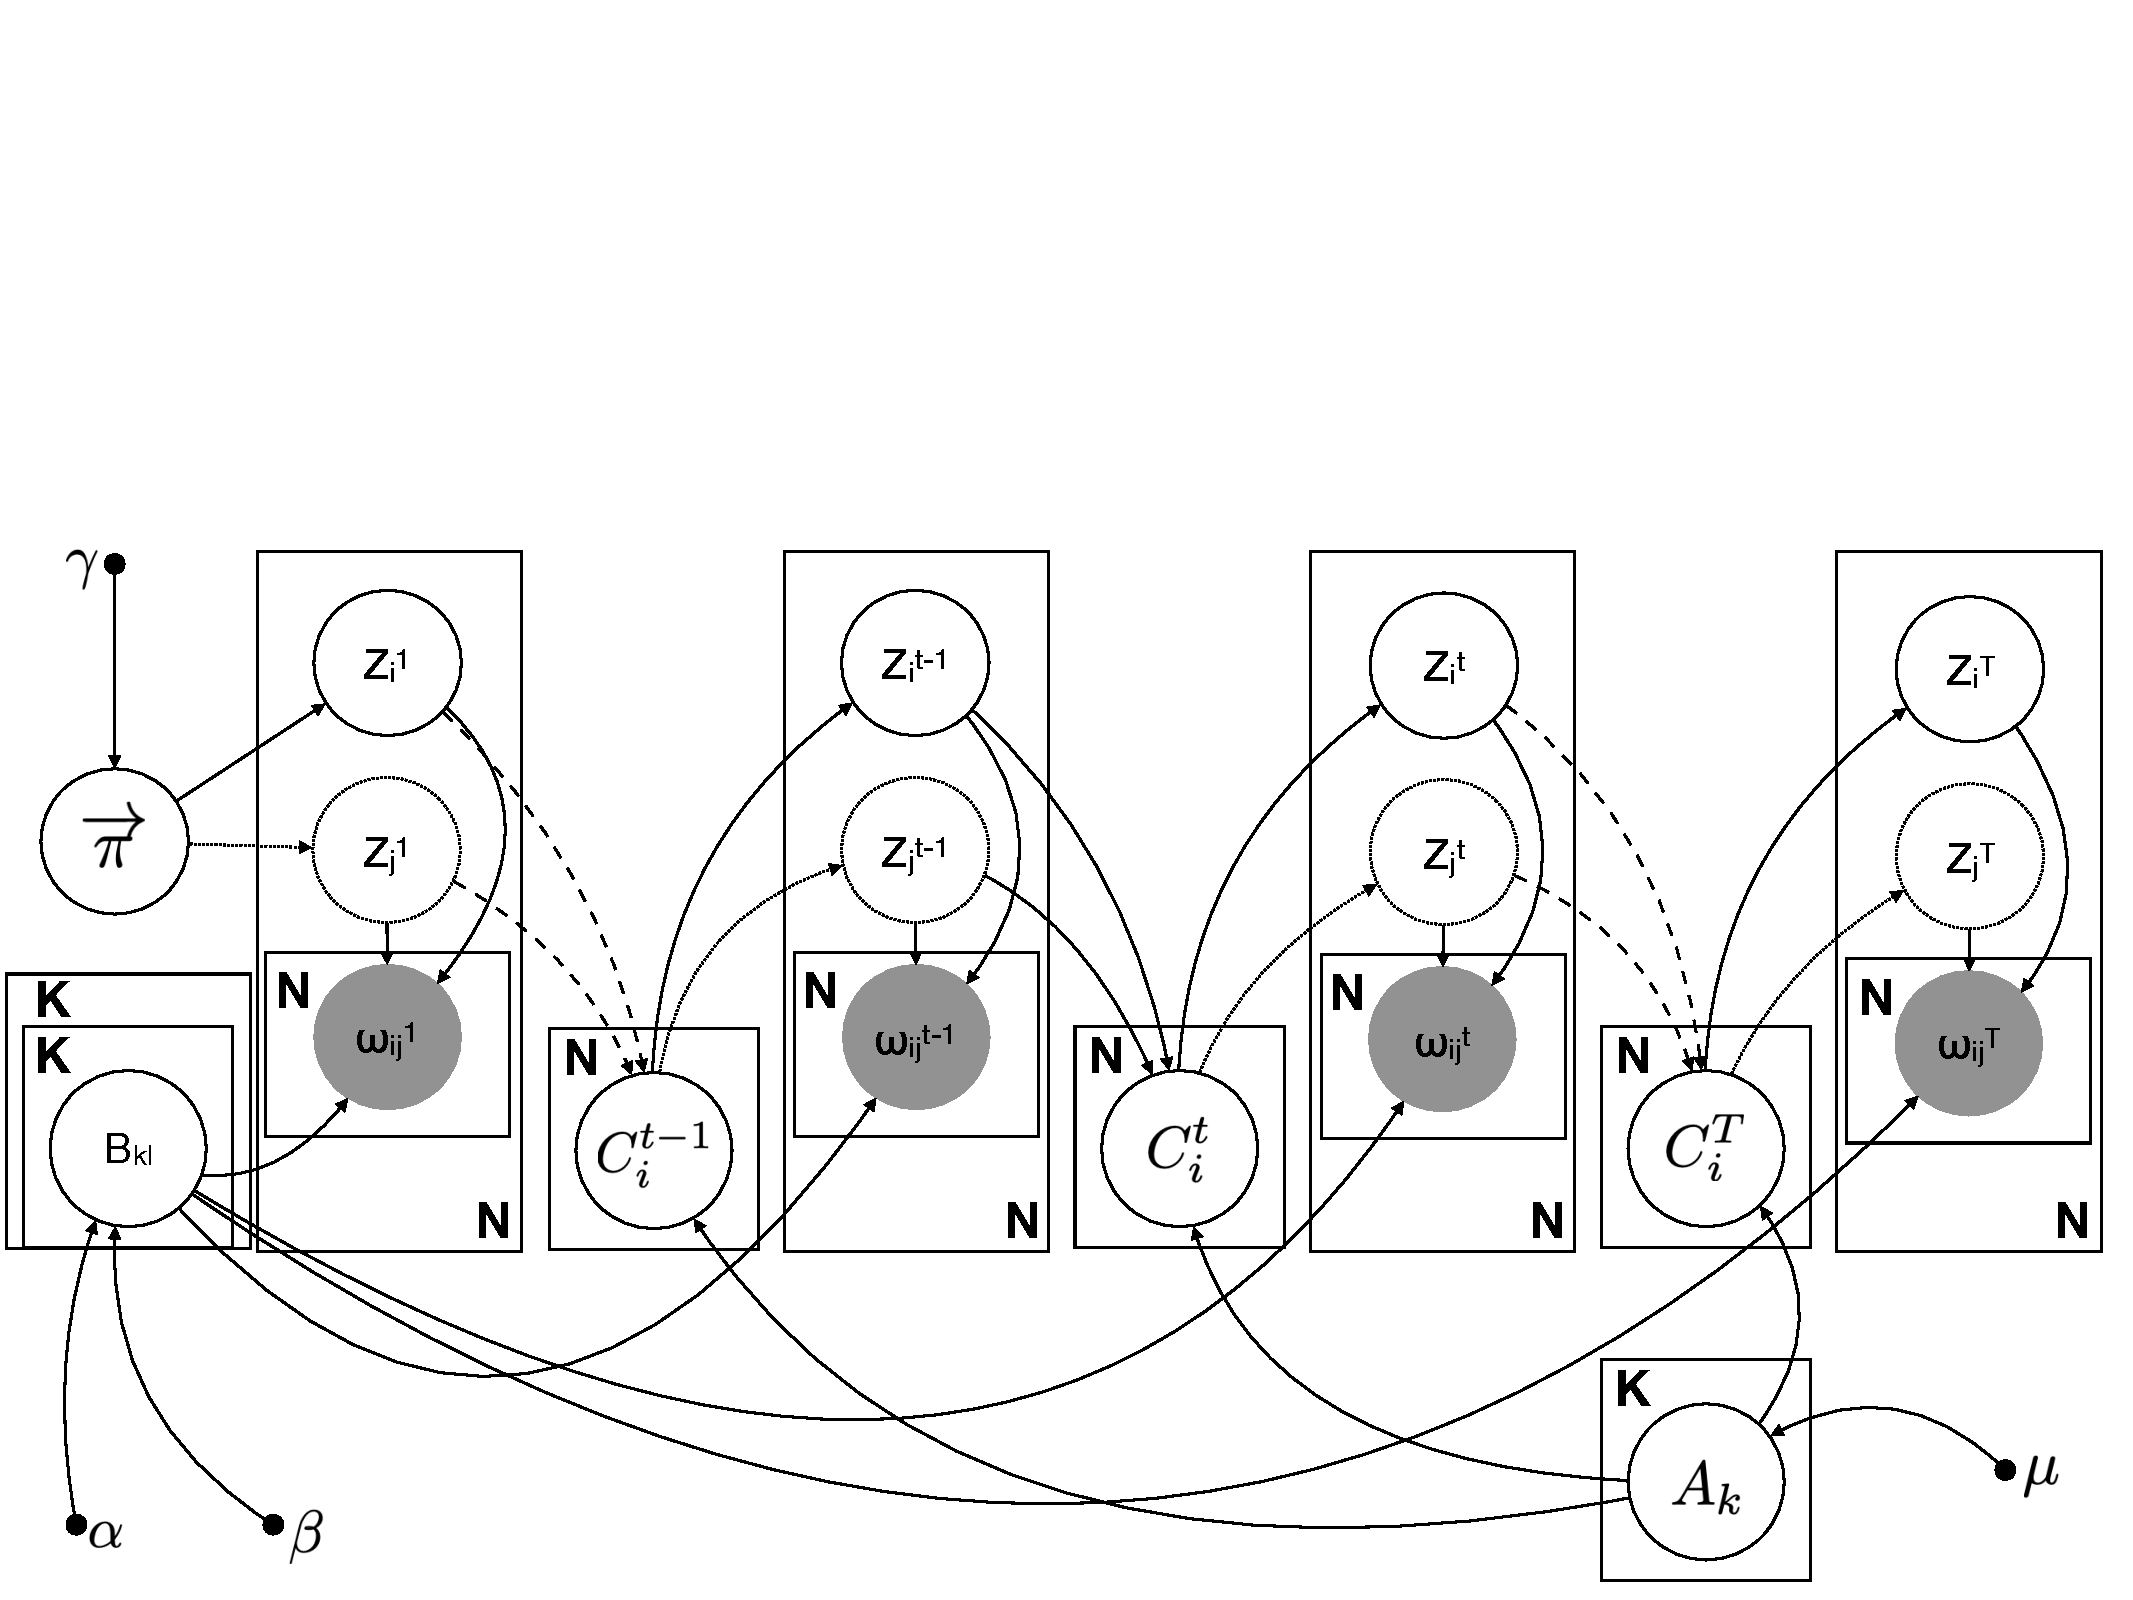
\includegraphics[width=.9\textwidth]{figures/chap04/graph-model_v3_cuted.pdf}
% 	\caption{HB-DSBM图模型}
% 	\label{fig.4.1}
% \end{figure}

% 本节首先介绍HB-DSBM的核心生成机制来揭示它是如何通过层次贝叶斯结构同时建模社团级别和节点级别的动态演化的,随后给出其产生社团结构和动态网络的生成过程。

% 如图~\ref{fig.4.1}的图模型所示,HB-DSBM首先令$\pi$表示$Z^1$的先验分布,同时$\pi$服从参数为$\gamma$的狄利克雷分布。$B$是不同社团间节点的连边概率,即类随机块模型中的块矩阵,例如$B_{kl}$即代表属于$k$社团和属于$l$社团的节点之间连边的概率。而$B$服从参数为$\alpha$和$\beta$的Beta分布。

% 本章中的$A \in [0, 1]^{K \times K}$表示社团级别转移倾向矩阵,$A$的每一行$A_k$都服从参数为$\mu$的狄利克雷分布,因此 $\sum_l A_{kl} = 1$。同时$C = \{ C^2, \cdots C^T \}$表示节点级别的社团转移倾向,每个$C^t$都是由社团级别转移倾向矩阵$A$生成。对于$t>1$的网络快照,任意节点$i$都有其唯一的转移向量 $C_i^t  \in [0, 1]^K$,该向量服从以参数为$A_{z_i^{t-1}}$的狄利克雷分布,因此$\sum_{k} C_{ik}^t = 1$。这一部分就是本模型的核心:层次狄利克雷生成机制。

% 基于以上机制,模型就可以生成社团标签以及动态网络中每个网络快照中的边。具体生成过程如下所示:
% \begin{enumerate}
% 	\item 生成初始社团划分概率 ${\pi} \sim Dir({\gamma})$
% 	\item 生成块矩阵 $B \sim Beta({\alpha},{\beta})$
% 	\item 对于网络快照$t=1$的每个节点$i$:
% 	\begin{enumerate}
% 		\item 生成每个节点的社团归属 $z_i^1 \sim Mult({\pi})$ 
% 		\item 生成每条边 $\omega_{ij}^1 \sim Bernoulli(\cdot | B_{z_i^1,z_j^1})$
% 	\end{enumerate}
% 	\item 生成每个社团级别转移矩阵的社团转移向量 ${A}_k \sim Dir({\mu})$
% 	\item 对网络快照$t>1$中的每个节点$i$:
% 	\begin{enumerate}
% 		\item 生成每个节点级别的社团转移向量${C}_i^t \sim Dir({A}_{z_i^{t-1}})$
% 		\item 生成每个节点的社团归属 $z_i^t \sim Mult({C}_i^t)$
% 		\item 生成每条边 $\omega_{ij}^t \sim Bernoulli(\cdot | B_{z_i^t,z_j^t})$
% 	\end{enumerate}
% \end{enumerate}

% 由生成过程可知,当$t=1$时,模型首先利用参数为$\pi$的多项分布生成$i$的社团归属$z_i^1$,随后以伯努利分布 $Bernoulli(\cdot|B_{z_i^1,z_j^1})$生成每对节点对$i,j$之间的连边。而当$t>1$时,$i$节点的社团归属由以参数为$C_i^t$的多项分布决定,即$z_i^t \sim Mult({C}_i^t)$。而$C_i^t$服从狄利克雷分布$Dir(A_{z_i^{t-1}})$。

% 根据如图~\ref{fig.4.1}的概率图模型和生成过程,可以写出HB-DSBM的联合概率分布如下:

% \begin{equation}
% \begin{split}
% Pr&(W_T,Z_T,C_T,B,A,\pi|\alpha,\beta,\gamma,\mu) \\
% = & \prod_{t=1}^T Pr(W^t | Z^t,B) Pr(Z^1|\pi) \prod_{t=2}^T Pr(Z^t|C^t) \\
% & \prod_{t=2}^T Pr(C^t|A,Z^{t-1}) Pr(A|\mu) Pr(\pi|\gamma) Pr(B|\alpha,\beta) \\
% \end{split}
% \end{equation}

% \section{模型求解}

% 本小结介绍针对本模型的高效的变分近似推断算法。
% \subsection{变分推断}
% 由于模型参数较多且复杂,直接推出模型后验$p(Z,C,B,A,\pi|W)$是困难的, 因此基于平均场理论,本节提出了用$q(Z,C,B,A,\pi)$ 来近似$p(Z,C,B,A,\pi|W)$. 为了简介,本节用$\Delta$ 来表示参数 $\{\pi,B,A,C,Z\}$. 更详细来说,即:

% \begin{equation}
% \label{eq2}
% \begin{split}
% & q(\Delta) =  \prod_{t=1}^T \prod_{i=1}^N q(z_i^t) \prod_{t=2}^T \prod_{i=1}^N q(c_i^t)q(B)q(A)q(\pi)  \\
% \end{split}
% \end{equation}

% 其中块矩阵变分参数$q(B|\widetilde{\alpha},\widetilde{\beta}) = \prod_{k,l\geq k} Beta(\widetilde{\alpha}_{kl},\widetilde{\beta}_{kl})$, 社团级别转移矩阵变分参数 $q(A|\widetilde{\mu}) = \prod_{k=1}^K \prod_{l=1}^K Dir(\widetilde{\mu}_{kl})$。 而社团归属变分参数$q(z_i^t|\widetilde{\phi}_i^t)$ 服从以$\widetilde{\phi}_i^t$为参数的多项分布。
% 而$q(c_i^t|\widetilde{\xi}_i^t)$和$q(\pi|\widetilde{\gamma})$都分别服从以$\widetilde{\xi}_i^t$和$\widetilde{\mu}_{kl}$为参数的狄利克雷分布。

% 因此有变分下界:
% %  \begin{equation}
% %  \begin{split}
% %     % & q(z_i^t|\widetilde{\phi}_i^t) \sim Multi(\widetilde{\phi}_i^t)\\
% %     % & q(c_i^t|\widetilde{\xi}_i^t) \sim Dir(\widetilde{\xi}_i^t)\\
% %     % & q(B|\widetilde{\alpha},\widetilde{\beta}) = \prod_{k,l\geq k} q(B_{kl}|\widetilde{\alpha}_{kl},\widetilde{\beta}_{kl})\\
% %     % & q(B_{kl}|\widetilde{\alpha}_{kl},\widetilde{\beta}_{kl}) = Beta(\widetilde{\alpha}_{kl},\widetilde{\beta}_{kl}) \\
% %     & q(B|\widetilde{\alpha},\widetilde{\beta}) = \prod_{k,l\geq k} Beta(\widetilde{\alpha}_{kl},\widetilde{\beta}_{kl}) \\
% %     & q(A|\widetilde{\mu}) = \prod_{k=1}^K \prod_{l=1}^K Dir(\widetilde{\mu}_{kl}) \\
% %     % & q(A|\widetilde{\mu}) = \prod_{k=1}^K \prod_{l=1}^K q(A_{kl} | \widetilde{\mu}_{kl})\\
% %     % & q(A_{kl} | \widetilde{\mu}_{kl}) \sim Dir(\widetilde{\mu}_{kl})\\
% %     % & q(\pi|\widetilde{\gamma}) = Dir(\widetilde{\gamma})\\
% %  \end{split}
% %  \end{equation}

% \begin{equation}
% \label{eq:3}
% \begin{split}
% &\widetilde{L}(q) = \sum_z \int_{\pi,B,A,C}q(\Delta) \log \frac{p(\Delta,W)}{q(\Delta)} 
% %  \end{split}
% %  \end{equation}
% %  By considering the constant
% %  \begin{equation}
% %  \begin{split}
% %      \widetilde{L}(q) = \log p(\pi,B,A,C,Z,W) - KL(q||p)
% %  \end{split}
% %  \end{equation}
% %  
% %  The ELBO is given by:
% %  \begin{equation}
% %  \begin{split}
% = E_{\widetilde{\phi},\widetilde{\alpha},\widetilde{\beta}} \sum_{t=1}^T [\log P(W^t|Z^t,B)] \\
% &+ E_{\widetilde{\gamma},\widetilde{\phi}}[\log P(Z^1|\pi)]+E_{\widetilde{\phi},\widetilde{\xi}} \sum_{t=2}^T [\log P(Z^t|C^t)] 
% + E_{\widetilde{\xi},\widetilde{\phi},\widetilde{\mu}} \sum_{t=2}^T [\log P(C^t|A,Z^{t-1})]\\
% &+ E_{\widetilde{\mu}}[\log P(A)]+E_{\widetilde{\gamma}}[\log P(\pi)] + E_{\widetilde{\alpha},\widetilde{\beta}}[\log P(B)]
% - E_{\widetilde{\gamma}}[\log q(\pi)] - E_{\widetilde{\alpha},\widetilde{\beta}}[\log q(B)]  - E_{\widetilde{\mu}}[\log q(A)]\\
% &- \sum_{t=2}^T \sum_{i=1}^N E_{\widetilde{\xi}}[\log q(C_i^t)] - \sum_{t=1}^T \sum_{i=1}^N E_{\widetilde{\phi}}[\log q(z_i^t)] \\
% \end{split}
% \end{equation}

% 这里 $\widetilde{\phi},\widetilde{\xi},\widetilde{\alpha},\widetilde{\beta},\widetilde{\mu},\widetilde{\gamma}$ 即为变分参数。为了方便起见,本章省略掉了分布的条件部分。 例如,本章将 $q(\Delta|\widetilde{\phi},\widetilde{\xi},\widetilde{\alpha},\widetilde{\beta},\widetilde{\mu},\widetilde{\gamma})$ 和 $q(z_i^t|\widetilde{\phi}_i^t)$ 略写为$q(\Delta)$和$q(z_i^t)$。
% 因此该模型的变分下界(ELBO)$\widetilde{L}(q)$被写成了如上式\ref{eq:3}。

% 随后通过最大化ELBO来获得最优的隐变量$Z,\pi,B,A,C$和模型参数$\gamma,\alpha,\beta,\mu$。 通过对不同的参数$\widetilde{\phi},\widetilde{\gamma},\widetilde{\alpha},\widetilde{\beta},\widetilde{\mu},\widetilde{\xi}$对$\widetilde{L}(q)$求偏导,并令导数为0求得每个参数的更新公式,即:
% \begin{equation}
% \begin{split}
% \nabla \widetilde{L}(q) = \{ \frac{\partial \widetilde{L}}{\partial \widetilde{\gamma}},\frac{\partial \widetilde{L}}{\partial \widetilde{\alpha}},\frac{\partial \widetilde{L}}{\partial \widetilde{\beta}},\frac{\partial \widetilde{L}}{\partial \widetilde{\mu}},\frac{\partial \widetilde{L}}{\partial \widetilde{\xi}},\frac{\partial \widetilde{L}}{\partial \widetilde{\phi}} \} = 0
% \end{split}
% \end{equation}

% 每个参数的结果如下所示:
% \textbf{对 $\widetilde{\gamma}$}:

% 包含$\widetilde{\gamma}$的ELBO如下所示:
% \begin{equation}
% \begin{split}
% & \widetilde{L}_{\widetilde{\gamma}} = E_{\widetilde{\gamma},\widetilde{\phi}}[\log P(Z^1|\pi)] + E_{\widetilde{\gamma}}[\log P(\pi)]- E_{\widetilde{\gamma}}[\log q(\pi)] \\
% & = \log{\frac{\prod_{k=1}^K \log \Gamma (\widetilde{\gamma}_k)}{\Gamma (\sum_k \widetilde{\gamma}_k)}} 
%  + \sum_{k=1}^K ( \gamma_k - \widetilde{\gamma}_k + \sum_{i=1}^N \widetilde{\phi}_{ik}^1)[\psi(\widetilde{\gamma}_k) - \psi(\sum_k \widetilde{\gamma}_k)]\\
% \end{split}
% \end{equation}

% 这里 $\psi(x) = \frac{\Gamma'(x)}{\Gamma(x)} = \frac{\,d \log \Gamma(x)}{\, dx}$. 
% 通过对$\widetilde{L}_{\widetilde{\gamma}}$ 针对$\widetilde{\gamma}$求偏导,并令导数等于0,得到其更新公式如下:
% \begin{equation}
% \label{eq4}
% \begin{split}
% \widetilde{\gamma}_k = \gamma_k + \sum_{i=1}^N \widetilde{\phi}_{ik}^1, \quad
% % \widetilde{\mu}_{kl} \propto \mu_l + \frac{\sum_{t=2}^T \sum_i \widetilde{\phi}_{ik}^{t-1}}{T-1}
% \end{split}
% \end{equation}

% \textbf{对于$\widetilde{\xi}$}:

% ELBO中包含$\widetilde{\xi}$的式子如下所示:
% \begin{equation}
% \begin{split}
% &\widetilde{L}_{\widetilde{\xi}} = E_{\widetilde{\phi},\widetilde{\xi}} \sum_{t=2}^T [\log P(Z^t|C^t)] 
% + E_{\widetilde{\xi},\widetilde{\phi},\widetilde{\mu}} \sum_{t=2}^T [\log P(C^t|A,Z^{t-1})] - \sum_{t=2}^T \sum_{i=1}^N E_{\widetilde{\xi}}[\log q(C_i^t)]\\
% \end{split}
% \end{equation}

% 利用同样方法求得更新公式如下所示:

% \begin{equation}
% \label{eq5}
% \begin{split}
% \widetilde{\xi}_{ik}^t \propto \widetilde{\phi}_{ik}^t + \sum_l \widetilde{\phi}_{il}^{t-1}(\frac{\widetilde{\mu}_{kl}}{\sum_l \widetilde{\mu}_{kl}} - 1) + 1
% \end{split}
% \end{equation}

% \textbf{对于参数$\widetilde{\alpha}$和$\widetilde{\beta}$}:

% ElBO中包含$\widetilde{\alpha}$和$\widetilde{\beta}$的式子如下所示:
% \begin{equation}
% \begin{split}
% &\widetilde{L}_{\widetilde{\alpha},\widetilde{\beta}} = E_{\widetilde{\phi},\widetilde{\alpha},\widetilde{\beta}} \sum_{t=1}^T [\log P(W^t|Z^t,B)] 
% - E_{\widetilde{\alpha},\widetilde{\beta}}[\log q(B)] + E_{\widetilde{\alpha},\widetilde{\beta}}[\log P(B)]\\
% &= \sum_{k \leq l} \log\{\frac{\Gamma(\widetilde{\alpha}_{kl})\Gamma(\widetilde{\beta}_{kl})}{\Gamma(\widetilde{\alpha}_{kl}+\widetilde{\beta}_{kl})}   \}  \\
% &+ \sum_{k=1}^K [\alpha_{kk}- \widetilde{\alpha}_{kk} +\sum_t \sum_{i < j} \widetilde{\phi}_{ik}^t\widetilde{\phi}_{jk}^t w_{ij}^t]
% [\psi(\widetilde{\alpha}_{kk})-\psi (\widetilde{\alpha}_{kk}+\widetilde{\beta}_{kk})] \\
% &+ \sum_{k=1}^K [\beta_{kk}- \widetilde{\beta}_{kk} +\sum_t \sum_{i < j} \widetilde{\phi}_{ik}^t\widetilde{\phi}_{jk}^t(1- w_{ij}^t)]
% [\psi(\widetilde{\beta}_{kk})-\psi (\widetilde{\alpha}_{kk}+\widetilde{\beta}_{kk})] \\
% &+ \sum_{k<l}^K [\alpha_{kl}- \widetilde{\alpha}_{kl} +\sum_t \sum_{i \neq j} \widetilde{\phi}_{ik}^t\widetilde{\phi}_{jk}^t w_{ij}^t]
% [\psi(\widetilde{\alpha}_{kl})-\psi (\widetilde{\alpha}_{kl}+\widetilde{\beta}_{kl})] \\
% &+ \sum_{k<l}^K [\beta_{kl}- \widetilde{\beta}_{kl} +\sum_t \sum_{i \neq j} \widetilde{\phi}_{ik}^t\widetilde{\phi}_{jk}^t(1- w_{ij}^t)]
% [\psi(\widetilde{\beta}_{kl})-\psi (\widetilde{\alpha}_{kl}+\widetilde{\beta}_{kl})] \\
% \end{split}
% \end{equation}

% 利用同样方法求得$\widetilde{\alpha}$和$\widetilde{\beta}$的更新公式如下:

% \begin{equation}
% \label{eq6}
% \begin{split}
% & \widetilde{\alpha}_{kk} = \alpha_{kk} + \frac{\sum_t \sum_{i<j} \widetilde{\phi}_{ik}^t \widetilde{\phi}_{jk}^t w_{ij}^t}{T}  \\
% & \widetilde{\beta}_{kk} = \beta_{kk} + \frac{\sum_t \sum_{i<j} \widetilde{\phi}_{ik}^t \widetilde{\phi}_{jk}^t (1-w_{ij}^t)}{T} \\
% & \widetilde{\alpha}_{kl} = \alpha_{kl} + \frac{\sum_t \sum_{i \neq j} \widetilde{\phi}_{ik}^t \widetilde{\phi}_{jl}^t w_{ij}^t}{T} \\
% & \widetilde{\beta}_{kl} = \beta_{kl} + \frac{\sum_t \sum_{i \neq j} \widetilde{\phi}_{ik}^t \widetilde{\phi}_{jl}^t (1-w_{ij}^t)}{T}  \\
% \end{split}
% \end{equation}

% \textbf{对于 $\widetilde{\mu}$}:

% ELBO中包含$\widetilde{\mu}$的式子如下所示:

% \begin{equation}
% \begin{split}
% & \widetilde{L}_{\widetilde{\mu}} = E_{\widetilde{\xi},\widetilde{\phi},\widetilde{\mu}} \sum_{t=2}^T [\log P(C^t|A,Z^{t-1})] 
% - E_{\widetilde{\mu}}[\log q(A)]+ E_{\widetilde{\mu}}[\log P(A)]\\
% &=\sum_{t=2}^T \sum_i \sum_k \sum_l \widetilde{\phi}_{ik}^{t-1} [\sum_l \psi(\widetilde{\mu}_{kl}) - \psi(\sum_l \widetilde{\mu}_{kl}) 
% + \frac{\widetilde{\mu}_{kl}}{\sum_l \widetilde{\mu}_{kl}}(\psi(\widetilde{\xi}_{ik}^t)-\psi(\sum_l \widetilde{\xi}_{il}^t))]  \\
% &-\log[\Gamma(\sum_l \widetilde{\mu}_{kl})] + \sum_l \log[\Gamma(\widetilde{\mu}_{kl})]
% + \sum_l (\mu_l - \widetilde{\mu}_{kl})[\psi(\widetilde{\mu}_{kl}) - \psi(\sum_l \widetilde{\mu}_{kl})]  \\
% \end{split}
% \end{equation}

% 因此有:
% \begin{equation}
% \label{eq7}
% \begin{split}
% \widetilde{\mu}_{kl} \propto \mu_l + \frac{\sum_{t=2}^T \sum_i \widetilde{\phi}_{ik}^{t-1}}{T-1}
% \end{split}
% \end{equation}

% \textbf{对于 $\widetilde{\phi}$}:

% $\widetilde{\phi}$ 是社团划分参数$Z$的变分参数,其更新公式随$t$的不同而不同。下面分情况讨论:

% \textbf{当$t=1$时}:

% ELBO中包含$\widetilde{\phi}$的项并考虑约束$\sum_k \widetilde{\phi}_{ik} = 1$,有:

% \begin{equation}
% \begin{split}
% &\widetilde{L}_{\widetilde{\phi}} = E_{\widetilde{\phi},\widetilde{\alpha},\widetilde{\beta}} [\log P(W^1|Z^1,B)] + E_{\widetilde{\gamma},\widetilde{\phi}}[\log P(Z^1|\pi)] \\
% &+ E_{\widetilde{\xi},\widetilde{\phi},\widetilde{\mu}}[\log P(C^2|A,Z^1)] - E_{\widetilde{\phi}}[\log q(Z^1)]+\rho (\sum_k \widetilde{\phi}_{ik}-1)\\
% \end{split}
% \end{equation}

% 因此有:

% %Here $\phi$ is the variational parameter of $Z$ with $T$ snapshot, we get the update rules of $\phi$ at different snapshots $t$ as follows.
% %When $t=1$:
% \begin{equation}
% \label{eq8}
% \begin{split}
% &\widetilde{\phi}_{ik}^1 \propto \exp\{\sum_j \sum_l \widetilde{\phi}_{jl}^1 [w_{ij}^1[\psi(\widetilde{\alpha}_{kl})-\psi(\widetilde{\alpha}_{kl}+\widetilde{\beta}_{kl})]
%   + (1-w_{ij}^1)[\psi(\widetilde{\beta}_{kl}) - \psi(\widetilde{\alpha}_{kl}+\widetilde{\beta}_{kl})] ]   \\
% & +[\psi(\widetilde{\gamma}_k)-\psi(\sum_l \widetilde{\gamma}_l) ] +[\sum_l \psi(\widetilde{\mu}_{kl}) - \psi(\sum_l \widetilde{\mu}_{kl}) 
% + \sum_l (\frac{\widetilde{\mu}_{kl}}{\sum_l \widetilde{\mu}_{kl}}-1)(\psi (\widetilde{\xi}_{ik}^2) - \psi(\sum_l \widetilde{\xi}_{il}^2))]  \} \\
% \end{split}
% \end{equation}

% \textbf{当$1<t<T$}:

% ELBO中包含$\widetilde{\phi}$的项,同时考虑$\sum_k \widetilde{\phi}_{ik} = 1 $,有:

% \begin{equation}
% \begin{split}
% & \widetilde{L}_{\widetilde{\phi}} = E_{\widetilde{\phi},\widetilde{\alpha},\widetilde{\beta}} [\log P(W^t|Z^t,B)]+E_{\widetilde{\phi},\widetilde{\xi}} [\log P(Z^t|C^t)]\\
% &+  E_{\widetilde{\xi},\widetilde{\phi},\widetilde{\mu}} [\log P(C^{t+1}|A,Z^t)]- \sum_{i=1}^N E_{\widetilde{\phi}}[\log q(z_i^t)]\\
% \end{split}
% \end{equation}
% %When $1<t<T$:
% 因此有:
% \begin{equation}
% \label{eq9}
% \begin{split}
% &\widetilde{\phi}_{ik}^t \propto \exp \{ \sum_j \sum_l \widetilde{\phi}_{jl}^t [w_{ij}^t[\psi(\widetilde{\alpha}_{kl}) - \psi(\widetilde{\alpha}_{kl}+\widetilde{\beta}_{kl})]
% + (1-w_{ij}^t)[\psi(\widetilde{\beta}_{kl})-\psi(\widetilde{\alpha}_{kl}+\widetilde{\beta}_{kl})]]    \\
% & + [\psi(\widetilde{\xi}_{ik}^t) - \psi(\sum_l \widetilde{\xi}_{il}^t)]+ [\sum_l \psi(\widetilde{\mu}_{kl}) - \psi(\sum_l \widetilde{\mu}_{kl}) 
% +\sum_l (\frac{\widetilde{\mu}_{kl}}{\sum_l \widetilde{\mu}_{kl}} -1)(\psi(\widetilde{\xi}_{ik}^{t+1}) - \psi(\sum_l \widetilde{\xi}_{il}^{t+1}))]  \}\\
% \end{split}
% \end{equation} 

% \textbf{当$t=T$}:

% ELBO中包含$\widetilde{\phi}$的项同时考虑约束$\sum_k \widetilde{\phi}_{ik} = 1 $,有:

% \begin{equation}
% \begin{split}
% & \widetilde{L}_{\widetilde{\phi}} = E_{\widetilde{\phi},\widetilde{\alpha},\widetilde{\beta}} [\log P(W^T|Z^T,B)]+E_{\widetilde{\phi},\widetilde{\xi}} [\log P(Z^T|C^T)]
% - \sum_{i=1}^N E_{\widetilde{\phi}}[\log q(z_i^T)]\\
% \end{split}
% \end{equation}
% %   When $t=T$:
% 因此有:
% \begin{equation}
% \label{eq10}
% \begin{split}
% &\widetilde{\phi}_{ik}^T \propto \exp \{ \sum_j \sum_l \widetilde{\phi}_{jl}^T [w_{ij}^T[\psi(\widetilde{\alpha}_{kl}) - \psi(\widetilde{\alpha}_{kl}+\widetilde{\beta}_{kl})] + \\
% &(1-w_{ij}^T)[\psi(\widetilde{\beta}_{kl})-\psi(\widetilde{\alpha}_{kl}+\widetilde{\beta}_{kl})]]  + [\psi(\widetilde{\xi}_{ik}^T) - \psi(\sum_l \widetilde{\xi}_{il}^T)]\}  \\
% \end{split}
% \end{equation} 
% % Here $\psi(x) = \frac{\Gamma'(x)}{\Gamma(x)} = \frac{\,d \log \Gamma(x)}{\, dx}$. 

% 由更新公式可知,模型超参数$\mu$和$\alpha$ 都为常量且其不影响模型结果。下面介绍得到更新公式后的迭代算法

% \subsection{迭代算法}

% 现在已经有了所有参数的更新公式,下面给出变分EM的更新算法如算法~\ref{alg4.1}所示。

% \begin{algorithm}
% 	\caption{HB-DSBM迭代算法}\label{alg4.1}
% 	\algorithmicrequire ~~ 动态网络邻接矩阵 $W$, 对大迭代次数 $n_{max}$ 和阈值变量$\varepsilon$ \\
% 	\algorithmicensure ~~ $\widetilde{\alpha},\widetilde{\beta},\widetilde{\gamma},\widetilde{\mu},\widetilde{\xi},\widetilde{\phi}$
% 	\begin{algorithmic}[1]
% 		\REPEAT
% 		\STATE 给定$\widetilde{\phi}$, 根据迭代公式~\ref{eq4}
% 		~\ref{eq5}~\ref{eq6}~\ref{eq7}更新 $\widetilde{\xi},\widetilde{\gamma},\widetilde{\alpha},\widetilde{\beta},\widetilde{\mu}$
% 		\STATE 给定 $\widetilde{\xi},\widetilde{\gamma},\widetilde{\alpha},\widetilde{\beta},\widetilde{\mu}$, 根据迭代公式\ref{eq8}~\ref{eq9}~\ref{eq10}更新 $\widetilde{\phi}$ 
% 		\UNTIL {$|\mathcal{L}^{new}-\mathcal{L}^{old}|<\varepsilon$ 或迭代次数 $> n_{max}$}
% 		\RETURN $\widetilde{\xi},\widetilde{\gamma},\widetilde{\alpha},\widetilde{\beta},\widetilde{\mu},\widetilde{\phi}$
% 	\end{algorithmic}
% \end{algorithm}

% 算法的复杂度依赖于三个部分。 更新$\phi$的复杂度是$O(TN^2K^2)$, 其中 $T$ 是网络快照的个数,  $N$ 网络中节点的数量,而$K$ 是社团的个数。 而更新 $\xi$的复杂度是$O(TNK^2)$。 最后ELBO的计算复杂度是$O(TN^2K^2)$.因此理论上该算法的复杂度是 $O(N^2)$. 而真实世界网络的数据往往是稀疏的,因此可以通过负采样或并行计算有效提升算法的运行效率,使其适应于大规模数据集。

% \section{实验及验证}

% 本小节将本文提出的算法HB-DSBM与四种同类动态网络社团检测算法在四个数据集(两个生成数据集与两个真实数据集)进行比较,以证明HB-DSBM的效果优于同类方法。同时在DBLP数据集中对HB-DSBM与DSBM进行社团演化分析,以证明本方法的社团演化分析更加细致且符合实际。
% \subsection{数据集}
% 本章实验使用四个数据集对HB-DSBM及对比方法进行比较,包括两个生成数据集和两个真实数据集,所有数据集均有真相。

% \textbf{data1} 由Lin 等人~\cite{lin2008facetnet}基于Girvan 和Newman提出的数据的改进版数据集。该数据集具有不同的参数设置,每个参数设置组生成的数据包含$10$个时间快照和$128$个节点,这些节点分别属于$4$个不同的社团,每个社团均包含32个节点。参数$\sigma$表示某社团内部的节点与其他社团的节点连边的数量的均值;而$nC$代表每个时间快照到下一个时间快照离开其原有社团的节点的数量;$aD$则表示每个节点的平均度。

% \textbf{data2}是由Greene等人\cite{greene2010tracking}提出的。该数据集融合了社团级别的事件使得其更接近真实世界数据,该数据集中的每个网络包含$1000$个节点,$15$的平均度和$50$的最大节点度。该数据集的社团个数有$20$到$50$不等,社团间连边的概率为$0.2$。值得一提的是,该数据集中的节点服从网络的power-law。

% \textbf{KIT-email}\cite{gorkedynamic}数据集是email收发网络,其节点代表电子邮箱账号。本文将该数据集视作无向无权网络,并将该数据集处理成网络快照形式的数据,分别以$2$或$3$个月为一个时间间隔。其节点数以及社团个数对应于这两个时间间隔分别为$138$、$170$和$23$、$25$。

% \textbf{DBLP}\cite{konect:2017:dblp-cite}数据是开源的论文数据集。本文选取了涉及计算机的三个领域的数据,包括数据挖掘(DM)、数据库(DB)和人工智能(AI)。时间跨度为$9$年,其中包括$1163$个节点和按领域划分的$3$个社团。本文将数据划分为$9$个网络快照,每个快照对应一年。

% \subsection{动态社团检测}
% 本小结社团检测实验选取了四种动态网络社团检测方法,分别为DSBM~\cite{yang2011detecting}、DYNMOGA~\cite{folino2014evolutionary}、Genlouvain~\cite{jutla2011generalized}和PisCES~\cite{liu2018global},这四种动态社团检测方法均为不同实现方式得到的高质量的动态网络社团检测算法。以上四个算法的参数设置均遵从其原论文的最优设置。而HB-DSBM的超参数如前文所述,均对模型效果影响不大,因此实验部分设置参数为当$k \neq l$时 $\alpha_{kl} = 1$,而当$k \neq l$时 $\alpha_{kk} = 10$;$\beta$的设置与$\alpha$相同; $\mu$的设置和$\gamma$相同, 即 $\mu_k = \gamma_k = \frac{1}{K}$,其中$1<k<K$。
% \subsubsection{评价指标}
% 本章实验部分使用标准化互信息指标(NMI)~\cite{gong2007machine}作为社团检测效果的评价指标,这也是目前大部分动态社团检测方法所使用的评价指标。NMI被设计为静态网络社团划分的评价指标,因此本章会在每个时间快照计算社团划分的NMI值。NMI被用作网络社团划分衡量指标需要知道网络社团划分的真相。令$C=\{C_1,...,C_K\}$表示网络社团划分的真相,令 $C'=\{C'_1,...,C'_K\}$代表待评估的社团划分,其中$C_k$和$C'_k$分别代表真相以及待评估的第$k$个社团的所有节点。则NMI的定义如下所示:

% \begin{equation}
% \begin{split}
% NMI(C,C')=\frac{\sum_{C,C'}p(C,C')\log \frac{p(C,C')}{p(C)p(C')}}{max(H(C)H(C'))}
% \end{split}
% \end{equation}

% 其中,$H(C)$和$H(C')$表示社团$C$和$C'$的熵。NMI的值在$0$到$1$之间。NMI的值越高,代表待评估的社团划分与真相越接近。



% \subsubsection{实验结果}

% 将HB-DSBM与DYNOMGA、DSBM、GenLou以及PisCES在不同数据集中进行NMI对比。在$data1$不同参数设置中的对比结果如图~\ref{fig.4.2}所示,HB-DSBM在图~\ref{fig.4.2}(a)中比效果最好的DSBM有大约明显的NMI提升,同时在图~\ref{fig.4.2}(d)中有$0.1$的NMI提升。虽然HB-DSBM在图~\ref{fig.4.2}(b)与图~\ref{fig.4.2}(c)中与其余方法的NMI提升差距不大,但是依然是效果最好的。HB-DSBM在五种方法中具有最好的NMI效果,证明该方法正确的把握住了节点演化的模式。HB-DSBM的曲线更加平滑,因为该模型结合了社团级别的演化以及节点级别的演化模式,成功的把握住了节点演化的异质性。DSBM的NMI曲线也比其他方法更加平滑,因为其融合了社团级别的演化模式,但是其忽略了同社团节点内演化模式的异质性。反观DYNOMGA和GenLou将社团检测与社团演化看做了两个独立的部分,因此其NMI曲线不够平滑,特别是在图~\ref{fig.4.2}(c)和图~\ref{fig.4.2}(d)中。而PisCES在不同时间快照中显示了很大的NMI反差,说明其对网络的噪声非常敏感。

% \begin{figure}[htbp]
% 	\centering
% 	\subfigure[$\sigma=4,nC=9,aD=16$]{
% 		\label{Fig.4.2.a}
% 		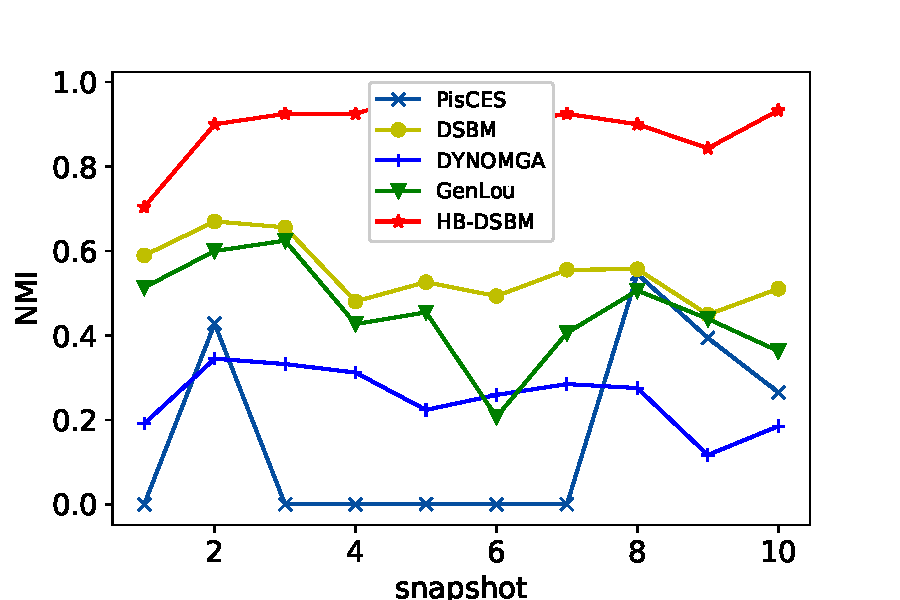
\includegraphics[width=.48\textwidth]{figures/chap04/compare4916.pdf}
% 	}
% 	\subfigure[$\sigma=4,nC=9,aD=20$]{
% 		% \label{Fig.vis.1}
% 		\label{Fig.4.2.b}
% 		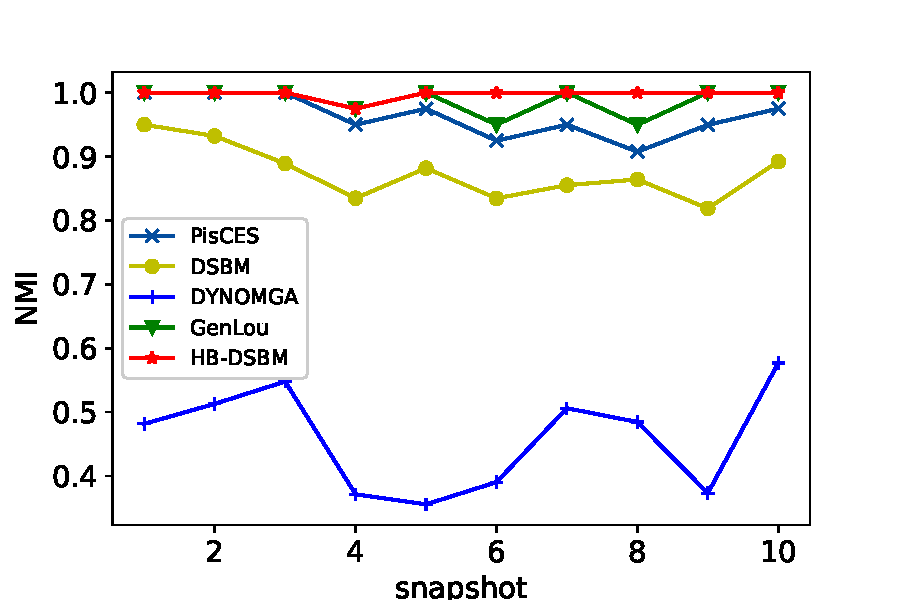
\includegraphics[width=.48\textwidth]{figures/chap04/compare4920.pdf}
% 	}
% 	\subfigure[$\sigma=5,nC=3,aD=16$]{
% 		% \label{Fig.vis.1}
% 		\label{Fig.4.2.c}
% 		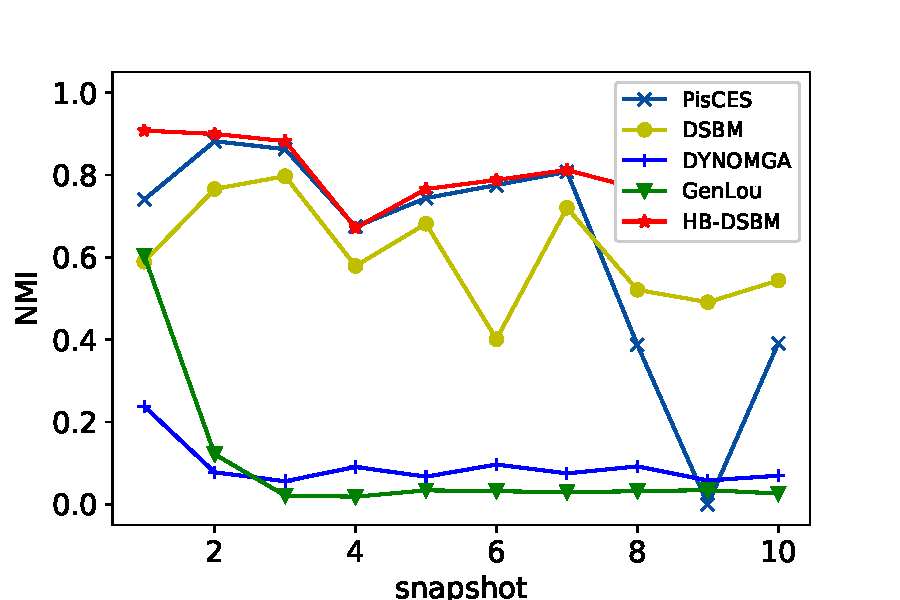
\includegraphics[width=.48\textwidth]{figures/chap04/compare5320.pdf}
% 	}
% 	\subfigure[$\sigma=5,nC=9,aD=20$]{
% 		% \label{Fig.vis.1}
% 		\label{Fig.4.2.d}
% 		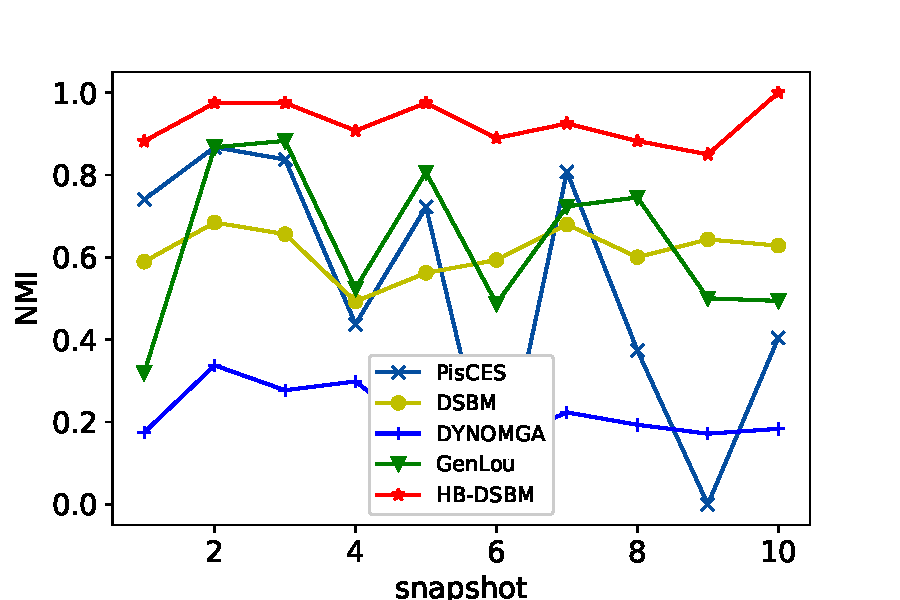
\includegraphics[width=.48\textwidth]{figures/chap04/compare5920.pdf}
% 	}
% 	\caption{$data1$四种不同参数设置的不同方法NMI对比。}
% 	\label{fig.4.2}
% \end{figure}

% 至于$data2$,NMI的结果显示如图~\ref{fig.4.3}所示,HB-DSBM依然具有最好的效果。在该数据集中,PisCES显示出比除HB-DSBM外其他方法更好的效果,而DSBM却显示除了最差的NMI表现,因为其利用吉布斯采样对模型进行求解,使得该模型在大规模数据中的有限次迭代中很难达到局部最优,即使是在每个网络快照$1000$个节点的数据集中。



% \begin{figure}[htbp]
% 	\centering
% 	\subfigure[扩展事件网络]{
% 		% \label{Fig.vis.1}
% 		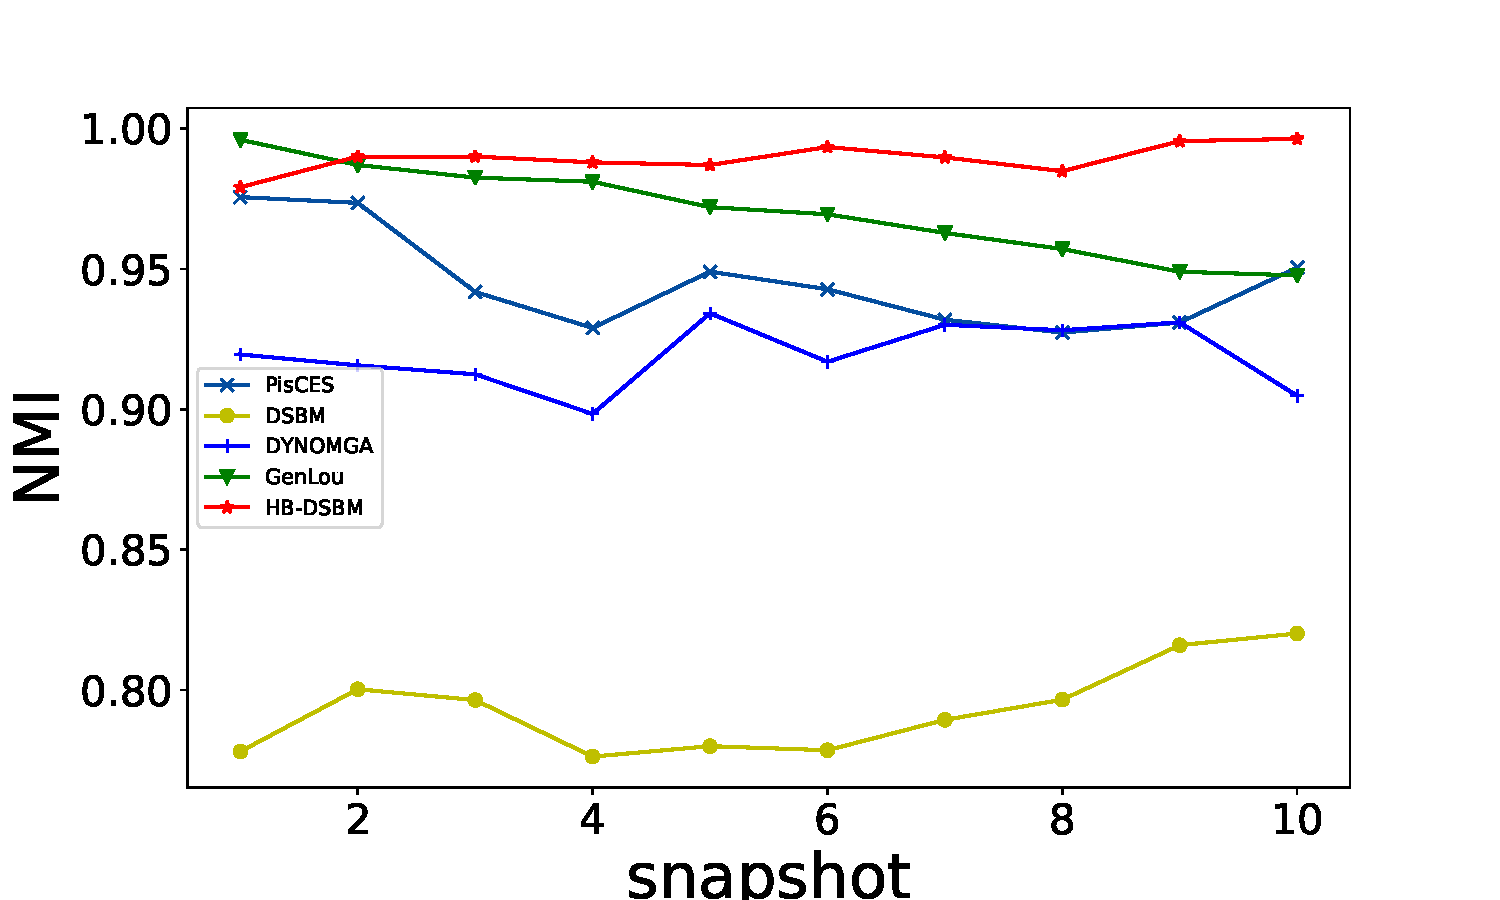
\includegraphics[width=.48\textwidth]{figures/chap04/asonexp11.pdf}}
% 	\subfigure[社团交换事件网络]{
% 		% \label{Fig.vis.1}
% 		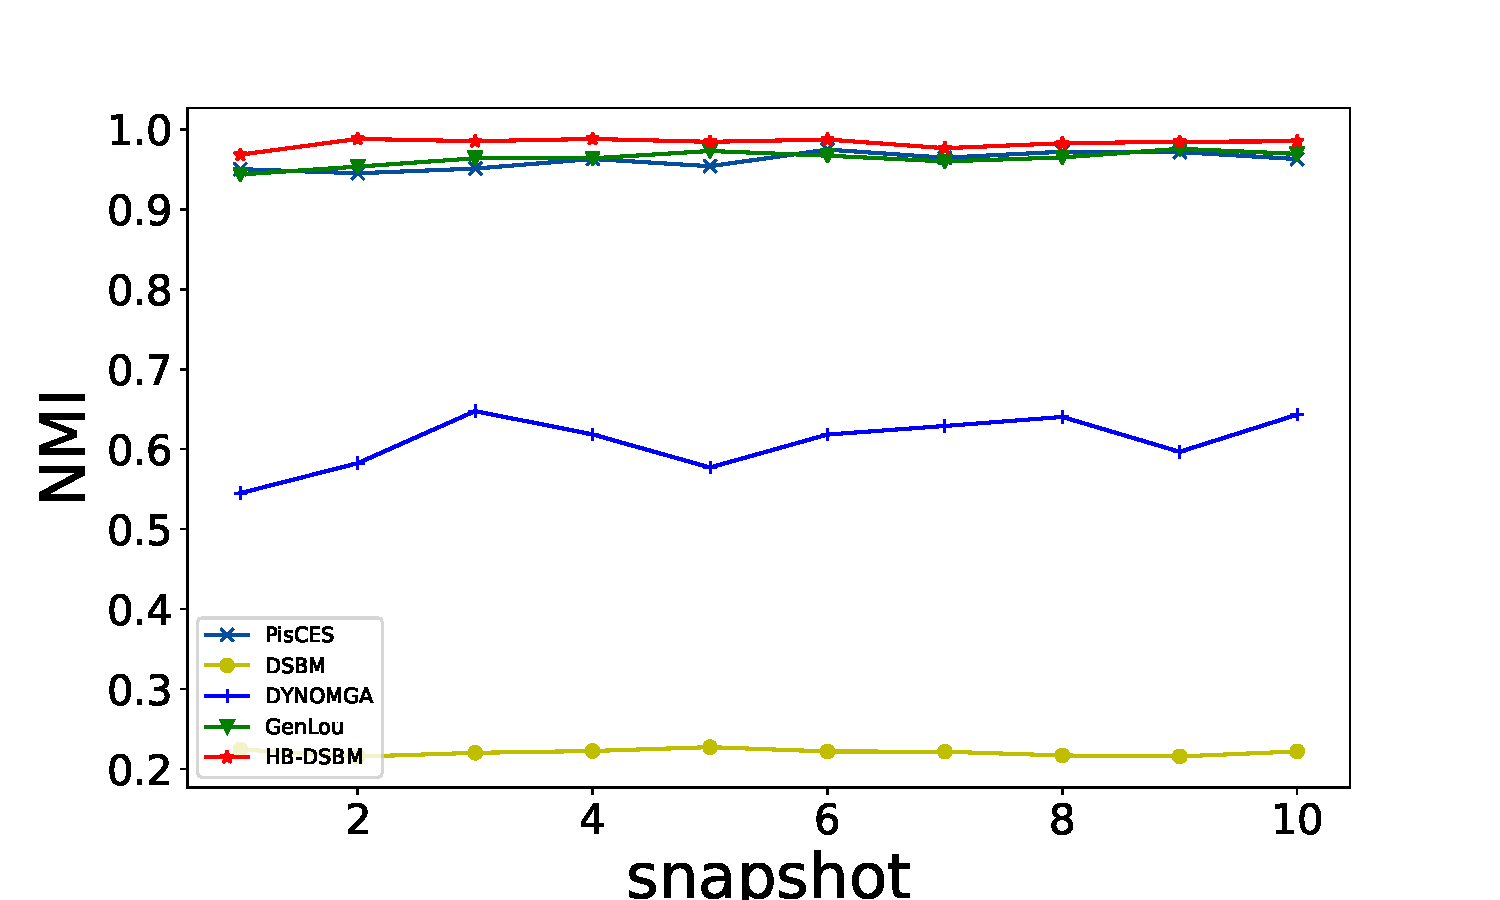
\includegraphics[width=.48\textwidth]{figures/chap04/swi1.pdf}
% 	}
% 	\caption{$data2$两个事件网络的不同方法NMI对比。}
% 	\label{fig.4.3}
% \end{figure}

% 真实世界数据集的实验如图~\ref{fig.4.4}~图\ref{fig.4.5}(a)所示,分别为KIT-email数据及DBLP数据。如图~\ref{fig.4.4}所示,HB-DSBM在KIT-email数据集中的NMI表现均高于其余方法,证明HB-DSBM不仅在生成数据集中具有较好表现,在真实世界数据集中也具有很好的社团检测效果。这里要强调的一点是,HB-DSBM在$t=1$的时候,效果并不比其余方法具有明显提升,因为HB-DSBM的改进主要注重在动态社团检测中节点的多层次演化,因此在第一个网络快照中的效果并不明显,而随着$t$的增长,HB-DSBM的效果会越来越好。




% \begin{figure}[htbp]
% 	\centering
% 	\subfigure[以两个月为间隔划分快照的网络]{
% 		% \label{Fig.vis.1}
% 		\label{fig.4.4.a}
% 		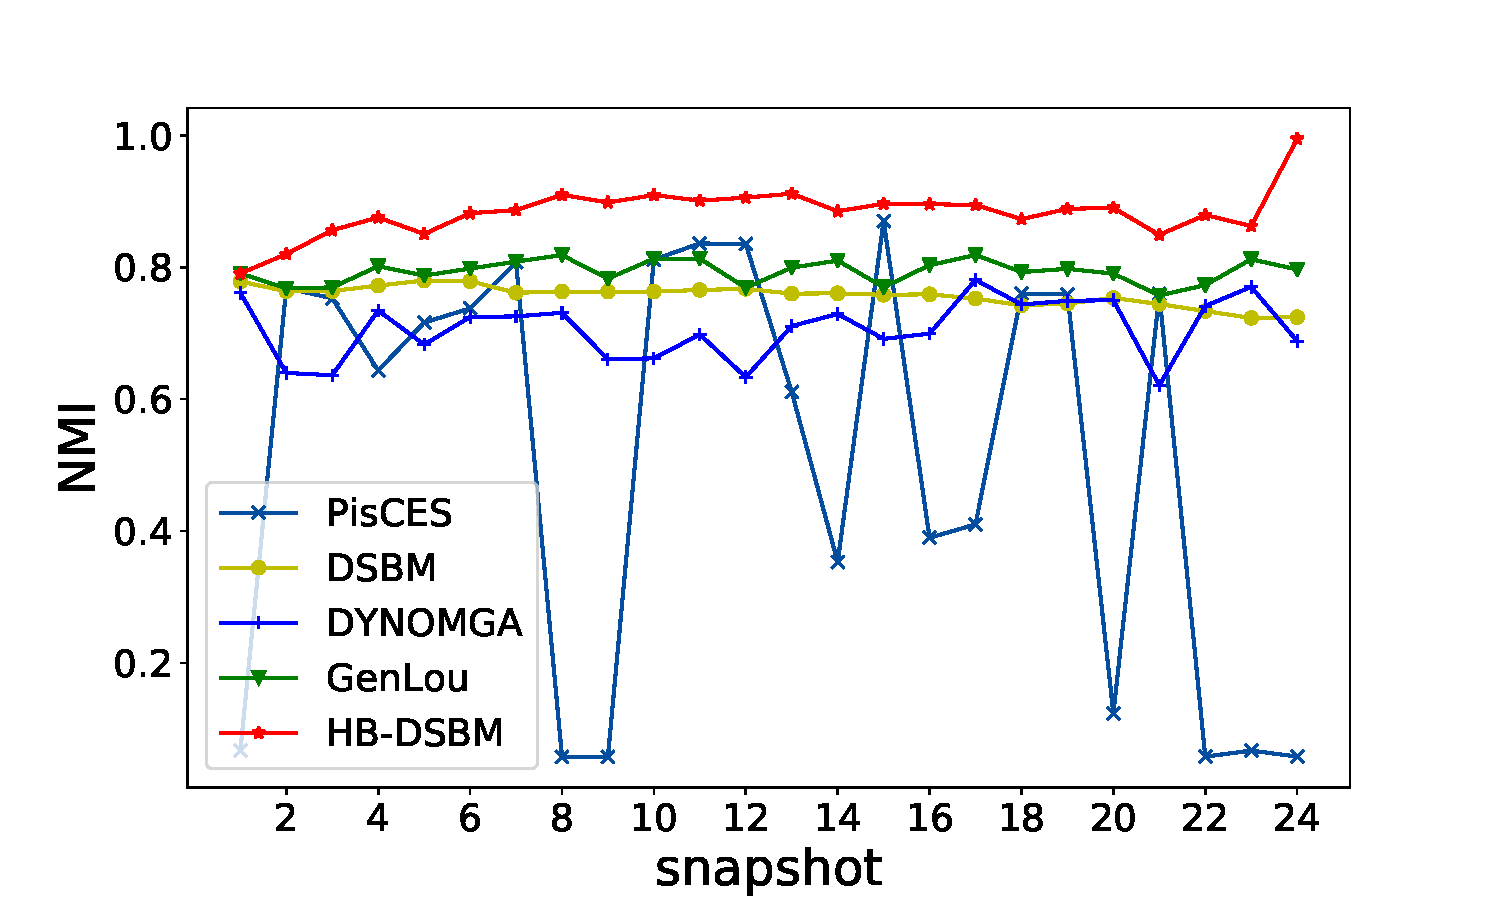
\includegraphics[width=.48\textwidth]{figures/chap04/compareInter2t.pdf}
% 	}
% 	\subfigure[以三个月为间隔划分快照的网络]{
% 		% \label{Fig.vis.1}
% 		\label{fig.4.4.b}
% 		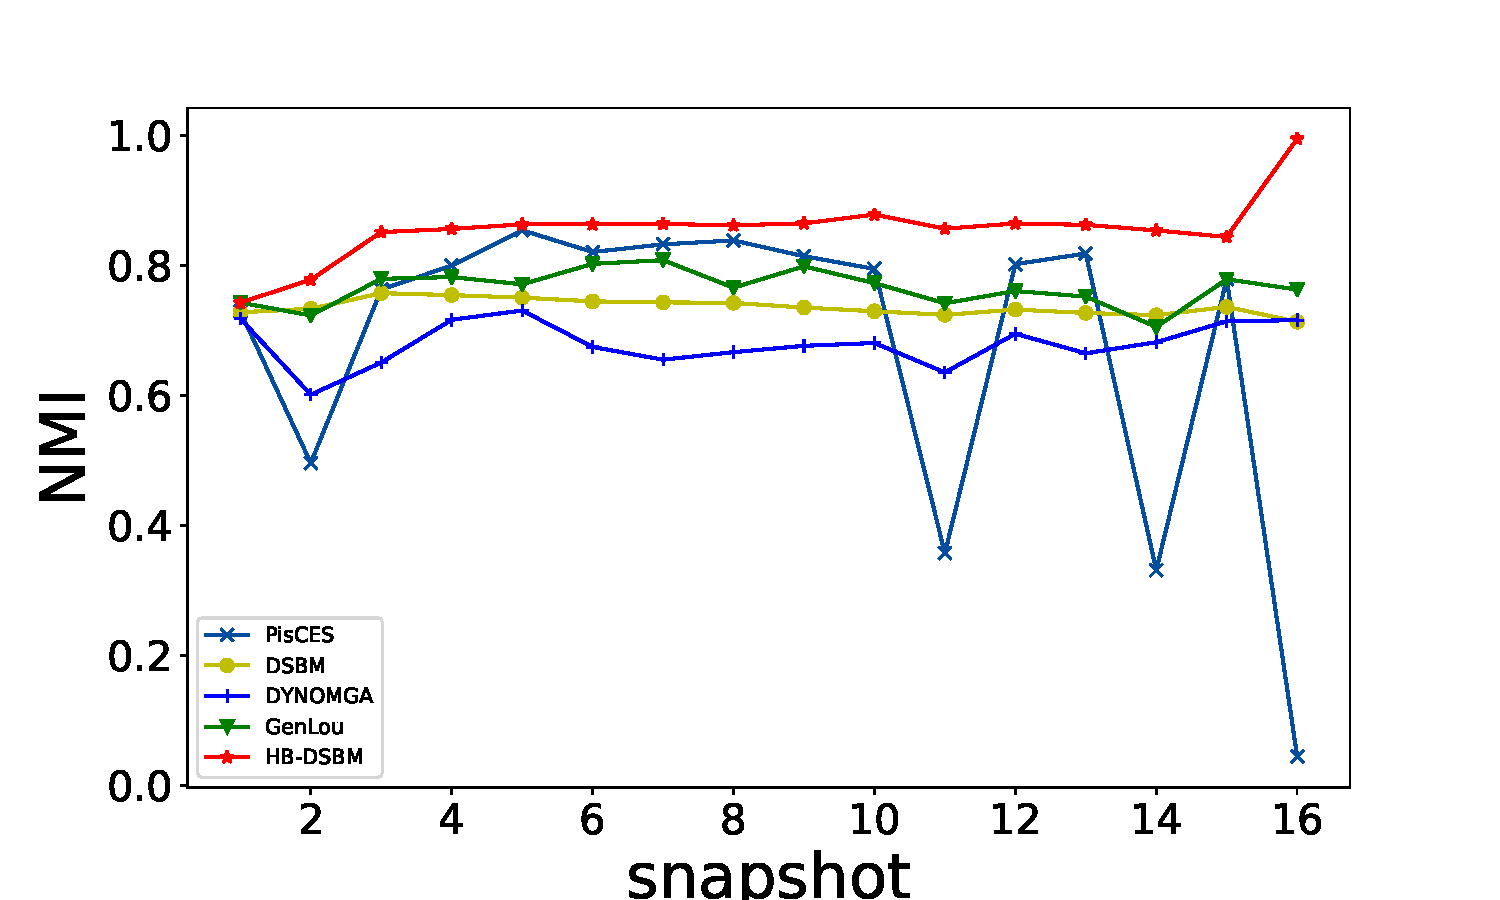
\includegraphics[width=.48\textwidth]{figures/chap04/compareInter3.pdf}
% 	}
% 	\caption{KIT-email数据不同时间间隔划分的切片网络的不同方法NMI对比}
% 	\label{fig.4.4}
% \end{figure}


% 而DBLP数据的同类方法对比如图\ref{fig.4.5}(a)所示,HB-DSBM的效果明显高于其他方法,再次证明了本模型的有效性。而DSBM的效果也优于其他方法,因为DSBM为生成模型,其同时融合了不同网络快照的社团检测与社团演化。而PisCES的噪声敏感性使得其在DBLP数据中的表现非常差,将所有节点划分到了同一个社团中。该数据集的不同方法NMI对比也再次证明了本文提出的动态网络社团演化层次贝叶斯结构的有效性。

% \begin{figure}[htbp]
% 	\centering
% 	\subfigure[DBLP数据的NMI对比]{
% 		\includegraphics[width=.48\textwidth]{figures/chap04/dblp_t6789.pdf}
% 		\label{Fig.4.5.a}
% 	}
% 	\subfigure[DBLP以及$data1$的社团转移矩阵可视化]{
% 		\includegraphics[width=.48\textwidth]{figures/chap04/communityHeatMap.pdf}
% 		\label{Fig.4.5.b}
% 	}
% 	\caption{DBLP数据社团检测及演化效果图。}
% 	\label{fig.4.5}
% \end{figure}


% \subsection{社团演化分析}

% 以往的模型如DSBM将在同一个社团的节点视作等价,也就是说在同一个社团的两个节点在模型中没有任何差别,它们具有相同的社团转移倾向,并且DSBM中的社团转移倾向矩阵并不会随着时间推移而变化。也就是说,以往的模型只考虑了节点的社团级别的演化倾向,并且是不变的。在HB-DSBM中,隐变量$C$和$A$分别代表了节点级别和社团级别的演化倾向,同时通过层次生成结构将这两个参数整合到了一起。模型社团级别的转移倾向矩阵$A$的可视化如图\ref{fig.4.5}(b)所示,图中分别展示了DBLP和$data1$的社团级别的转移倾向。然而社团级别的转移倾向并不是一成不变的,社团级别的转移倾向会随着时间变化,如图\ref{fig.4.6}可以看到,HB-DSBM准确把握住了不同网络快照中的社团级别的节点社团转移倾向。

% \begin{figure}[htbp]
% 	\centering
% 	\includegraphics[width=.8\textwidth]{figures/chap04/communityHeatMapt.pdf}
% 	\caption{基于HB-DSBM模型的社团级别转移矩阵$A$分别在DBLP和$data1$数据的可视化(上半部分)与真实社团转移真相的可视化(下半部分)之间的对比。}
% 	\label{fig.4.6}
% \end{figure}


% 而同一社团的节点也具有不同的社团转移倾向,图\ref{fig.4.7}展示了DBLP数据中不同研究领域的作者的研究兴趣领域发生转移的倾向的异质性。例如,$Theo Gevers$在$2009$年发表了一篇数据挖掘的论文。根据模型的节点转移矩阵的计算,他有很大的倾向继续在数据挖掘领域发表论文,而事实也验证了模型的推算。
% \begin{figure*}[htbp]
% 	\includegraphics[width=\textwidth]{figures/chap04/nodes_compare.pdf}
% 	\caption{DBLP数据集中部分节点($2009-2010$年)的社团转移倾向可视化(基于节点级别转移倾向参数$C$)。每个柱状图代表一个节点的转移倾向,从左到右分别为DM,DB,AI。所有柱状图共三行,每行代表一个领域,从上到下分别为DM,DB,AI。灰色的柱状图代表节点社团转移倾向与其所在社团转移倾向一致,而蓝色的柱状图代表节点的转移倾向与其所在社团的转移倾向不一致。}
% 	\label{fig.4.7}
% \end{figure*}

% 通过HB-DSBM对DBLP数据的分析,本文还发现了一个有趣的现象,即大部分作者都倾向于在几年之内转换他们的研究兴趣领域。换句话说,只有很少一部分的作者会长期停留在同一个研究领域。如图\ref{fig.4.8}所示,$Svetlana Lazebnik$倾向于每两年转换一次研究兴趣领域,而这个时间间隔对$Jing Peng$来说则为三年。同时$Andrew W. Fitzgibbon$从数据挖掘在$t=7$时将研究领域转移到了人工智能领域。$Amnon Shashua$则将研究兴趣领域从人工智能转移到数据挖掘进行研究,四年后又将研究兴趣领域转移回了人工智能。

%  \begin{figure}[htbp]
%  	\centering
% 	\includegraphics[width=.9\textwidth]{figures/chap04/nodes_evoluton1.pdf}
% 	\caption{DBLP数据选取的五个作者($Amnon Shashua, Anat Levin, Jing Peng, Andrew  W. Fitzgibbon, Svetlana Lazebnik$)的$8$年的转移倾向可视化。每个柱状图代表作者的社团转移倾向矩阵,从左到右分别为DM,DB,AI。}
% 	\label{fig.4.8}
% \end{figure}

% 为了衡量HB-DSBM在大数据集上的处理能力,本文将HB-DSBM和几个经典方法的运行效率进行了对比。数据集由著名的Dynamic Gervain Newman生成图算法进行生成,每个数据集有两个时间片,每个时间片具有不同的节点。图~\ref{fig.4.9}展示了HB-DSBM与对比方法在不同节点数据集上的运行时间的对比,图中可以看到,随着节点数的增加,PisCES与DSBM的计算用时超越了其他算法,效率变得很慢。值得一提的是,PisCES在每个时间片节点个数为$8192$时用时最长的同时,算法超过了最大迭代次数未收敛。而加入了随机采样模块后,变分推断结合随机采样的HB-DSBM随着节点数的增加,计算时间逐渐低于DSBM。可以看到,HB-DSBM的计算耗时曲线基本为线性增长,因此对于大规模数据集具有一定的处理能力。而PisCES与DSBM则接近于指数增长。运行速度最短的算法包括DYNMOGA与Genlouvain方法,而实际上,Genlouvain方法在对节点数为$8192$的动态网络进行社团检测时,由于内存不足导致了算法异常终止(Linux系统$16$G内存)。因此Genlouvain算法在实际使用时需要具有足够大的内存。而DYNMOGA算法使用了多目标优化的策略对动态网络进行社团检测,这种策略使得其算法可以多点并行,因而其运行速度凌驾于其他算法之上。受此启发,HB-DSBM也可以在后期加入并行计算,以此来进一步提升算法的运行效率。

%  \begin{figure}[htbp]
% 	\centering
% 	\includegraphics[width=.9\textwidth]{figures/chap04/performance.png}
% 	\caption{HB-DSBM与baseline方法在不同节点数的动态网络中的运行时间对比,横坐标为节点数,纵坐标为运行时间(s)。}
% 	\label{fig.4.9}
% \end{figure}

% \section{本章小结}
% 本章介绍了层次贝叶斯动态随机块模型,其层次贝叶斯生成结构能够同时融合节点级别以及社团级别的社团演化模式。同时本文利用变分推断对模型参数进行估计,利用合理的优化策略,模型可以适应大规模数据的计算。同类方法的对比也显示出HB-DSBM在动态网络社团检测任务中更加高效准确。


% !Mode:: "TeX:UTF-8"
\baselineskip 20pt
%-------------------------------------------------------------------------
%\chapter{个性化信息感知的评论摘要生成}
\chapter{融合节点流行度的动态网络建模及层次异常检测}
\label{chap:5}

%上一章提出了针对动态网络节点的社团转移异质性的层次贝叶斯建模方法HB-DSBM,并利用变分推断进行了模型参数求解,通过真实数据的社团检测任务证明了所设计的层次狄利克雷生成结构有效地建模了以社团为介观结构的动态网络生成机制,并从社团到节点的生成机制设计建模了节点的社团演化异质性。HB-DSBM的节点社团转移异质性的生成机制设计主要从生成的角度构建了从社团到节点的社团转移倾向的层次狄利克雷分布,并未与节点本身的特征直接建模,这对动态网络后续分析会造成一定困难。另外,生成模型从网络生成的角度对动态网络进行建模,其本质是刻画了网络的生成和演化机制,因此此类模型应该能够适配大部分下游任务,而HB-DSBM所提出的节点演化异常指数无法直接评估社团、网络在演化层面的异常。
本章将针对动态网络高阶生成机理显式建模问题进一步完善基于动态随机块模型的动态网络建模方法,使其能够刻画节点拓扑及演化异质性,并从演化分析能力提升层面提出针对动态网络的演化异常检测任务提出涵盖动态网络快照-社团-节点的异常检测方法,在真实数据集中进行了应用,以验证本章提出的方法在动态网络建模与应用的有效性。



\section{引言\label{chap5:intro}}

生成模型通过设计动态网络的生成机制,刻画了复杂系统从宏观到微观的生成和演化模式,而社团作为动态网络生成机制中的介观结构,承载了对动态网络生成机制建模的重要角色\cite{ghoshal2021influence},在对动态网络生成机制建模过程中起到承上启下作用,融入社团结构的生成模型往往能够刻画动态网络更加深层次的演化模式。例如,动态随机块模型在对网络进行建模后,可以通过社团归属参数对动态网络社团演化进行分析,挖掘所检测社团的扩张、收缩等时序变化\cite{yang2011detecting}。这使得该模型成为经典的复杂网络生成模型之一而获得了部分研究者的青睐。

近年来,部分研究者针对随机块模型在静态网络中存在的问题进行了改进。例如,针对经典随机块模型对网络中节点异质性建模缺失问题所提出的度修正随机块模型DCSBM\cite{ma2021determining}通过引入节点的度对网络中节点的连边概率进行修正;针对动态随机块模型的重叠社团建模缺失问题所提出的混合随机块模型MMSB\cite{godoy2016accurate}通过提出混合参数来刻画节点属于多个社团的场景。也有研究者考虑随机块模型在不同类型网络中的应用对其进行扩展,例如对属性网络进行适配的NEMBP算法\cite{he2017joint}、对超图进行适配的DCHSBM算法\cite{10214123}等进行适应性的改进与推理等。

上述方法并不适配动态网络,未考虑针对动态网络时序变化进行建模。Yang等人针对动态网络首先提出了动态随机块模型DSBM\cite{yang2011detecting},其改进自经典随机块模型SBM,并引入社团转移矩阵来建模动态网络节点的社团划分随时间的变化;Tang等人107则引入了狄利克雷过程来实现对动态随机块模型的模型选择,即自动确定社团个数;dMMSB\cite{xing2010state}则通过引入逻辑正态先验将混合随机块模型扩展到了动态网络;PDC-SBM\cite{riverain2023poisson}则考虑了动态网络边生成过程中的度异质性问题,引入了度修正参数以提升模型对动态网络的建模精度。

上述方法从经典随机块模型出发,在建模能力与适用性方面将随机块模型进行了改进,但依然存在一定缺陷。首先,在建模能力方面虽然以PDC-SBM为代表的方法从节点度异质性层面建模了动态网络中的节点异质性,但从前文的数据挖掘工作中可以看出,节点的度异质性并不适用所有网络;其次,以DCHSBM为代表的方法从网络类型适用性方面提升随机块模型的应用能力,但并未从任务层面对随机块模型进行扩展,最具代表性的任务即为异常检测。


%已有的方法仅验证模型建模方面的贡献,而忽略了生成模型本身对下游任务的通用性,即使验证了,也忽略了重要的下游任务---异常检测。
异常检测是数据挖掘和模式识别的重要任务之一~\cite{chandola2009anomaly,he2024diffusion},其目的就是寻找数据的正常模式中隐藏的不常见模式,即“离群点”。异常检测吸引了大量研究,并已广泛应用于多个领域,如欺诈检测~\cite{ahmed2016survey}和异常行为检测~\cite{amraee2018anomaly}。因此,近年来提出了多种方法。由于复杂网络可以用于建模众多现实世界系统,从国际航空运输~\cite{kasai2016network}到团队协作网络~\cite{dai2024gated},从社交网络~\cite{singh2024social}到引用网络~\cite{yan2024modeling},近年来,网络异常检测也受到了广泛关注,成为当前研究中的关键问题之一。与一般的异常检测类似,但有所超越,复杂网络中的异常检测通常指的是寻找那些模式显著偏离网络绝大多数节点的节点~\cite{lim2024future,li2024unsupervised},或是触发网络在不同层次(即微观层次、中观层次和宏观层次)发生显著结构变化的节点~\cite{hayat2024deep}。



由于网络结构本身随时间演化(动态或时间网络)\cite{huang2015triadic},例如节点的增加和消失以及边的变化,这些因素也驱动了社团的动态行为。因此,确定动态网络中的变化是正常还是异常变得非常困难。网络异常的原因也非常复杂,异常的形式多种多样,包括异常节点、异常边、异常子图以及变化点检测\cite{ranshous2015anomaly}。与此同时,动态网络中的异常检测有助于更好地理解网络的演化状态,评估网络的异常程度及其影响,并制定有效的干预措施来应对网络中的潜在危机。例如,通过适当使用异常检测来发现由网络演化引起的非平稳演化时间点,可以提高社团检测的准确性。它还可以应用于生物系统中的异常基因识别、气候预测和金融市场等领域。

一般来说,大多数现有的异常检测方法通常基于特定的视角,即分别在宏观、微观和中观层次上追踪动态网络在不同时间的演化,忽略了这三个层次上异常的相互影响。例如,FALCON~\cite{10597831} 聚焦于微观层次的异常检测(即异常节点或边),QRDN-ZNN~\cite{LI2025107412} 聚焦于神经网络的异常检测,以改进收敛性能,TCDformer~\cite{wan2024tcdformer} 聚焦于宏观层次的异常检测(即变化点)。事实上,在网络演化过程中,多个类型的异常同时发生是很有可能的,并且不同层次上的异常之间是相关的,在一个层次上的异常检测也有助于其他层次上的异常检测。以金融市场中的异常检测为例。在一个金融交易网络中,节点是账户,边是账户之间的交易。那么,微观层次的异常事件可以是与不同社团频繁交易的节点。在现实生活中,该账户可能是正常账户,也可能是用于欺诈的账户。


在中观层次上,异常事件可以是一些账户之间频繁交易,随后突然分裂成两个或更多的群体。这些账户在现实生活中可能属于一个大型公司,这一分裂事件可能表明该公司已经进行了重组。在宏观层次上的异常事件是整个市场发生了剧烈波动,这在金融市场网络中表现为网络变化的一个节点。此外,异常账户的积累可能导致账户群体发生剧变,整个市场的大事件可能会影响所有账户群体和账户(如金融危机)。如图~\ref{fig:example}所示,网络中节点$v_{7}$的状态随时间不断变化,因此它可以被视为整个网络演化中的异常点。换句话说,它的异常导致了整个网络的异常。然而,$v_{7}$的异常也可以视为中观层次异常的结果(即社团的分裂和合并)。这导致了网络演化过程中微观层次(异常节点)和中观层次(异常子图)异常的耦合。因此,可以看出,不同层次的异常之间是有相关性的,在一个层次上的异常检测也有助于其他层次上的异常检测。仅仅考虑单一类型的异常不足以支持网络演化规律的全面挖掘。换言之,网络在宏观、微观和中观层次上的异常是相互关联的,并且受到更深层次因素的驱动。异常只是表象,背后的本质尚未揭示。

\begin{figure}[htbp]
    \centering
    \includegraphics[width=.85\linewidth,trim=0.1in 0.5in 0.1in 0.1in]{figures/chap05/chap5motivation.png}
    \caption{动态网络各层次演化异常样例}
    \label{fig:example}
\end{figure} 





只有少数启发式方法考虑了不同层次异常之间的相关性,例如SCOUT~\cite{hulovatyy2016scout}和MDL~\cite{cheung2020simultaneous}同时检测社团结构异常和网络快照变更点。然而,它们仅考虑了部分而非所有层次的异常,且有些方法需要手动定义特征。此外,这些方法没有统一的框架,它们通过逐步实现不同层次的异常检测,无法建模异常之间的耦合关系,也无法实现异常之间的相互增强。为了捕捉不同层次异常之间的相关性,并更好地检测节点、社团、网络快照的异常,本章采用了统一的生成模型来建模动态网络,以探索不同尺度的异常行为~\cite{wang2019nodes,cheng2008robust}。 

% 异常检测是xxxx 接下面的

% 前文描述的HB-DSBM存在xxx问题,因此本文基于该模型设计了动态网络层次建模方法GEABS并提出了基于该模型参数的异常检测插件,扩展了该模型的下游应用。

% 另一方面,动态网络生成模型建模了网络在生成与演化过程中的复杂机制,此类模型能够支撑动态网络的多种下游任务。例如,前文描述的HB-DSBM模型中,通过拟合社团归属$z$的先验分布$Mult(\pi)$,即可确定网络中任意节点的社团划分;拟合模型中的伯努利分布$Bernoulli(·|B)$,即可预测网络中任意两个节点的边。然而对于网络中的
具体而言,本方法利用生成模型良好的可解释性来探讨异常的本质。本章将节点的流行度、社团成员关系等参数表示为随机块模型(SBM),通过节点流行度来刻画动态网络中节点的异质性,并基于模型参数设计了节点-社团-网络多层异常的检测指标,依次扩展随机块模型在动态网络中任务层面的适用范围。

本章的主要贡献可以概括如下:


\begin{itemize} 
    \item[$\bullet$] 本章提出基于随机块模型的动态网络建模方法GEABS(\textbf{G}eneration model to analyze the dynamic network for \textbf{E}xploring the \textbf{A}bnormal \textbf{B}ehaviors of different \textbf{S}cales),该方法通过建模动态网络节点-社团-网络快照的层次演化模式,并融入节点流行度参数刻画了节点的动态演化行为与拓扑异质性,以提升模型对于动态网络的建模能力。
    \item[$\bullet$] 利用熵与高阶距离度量等指标,结合模型刻画的网络参数,分别设计了网络 、社团、节点的多层次异常检测指标,扩展了本模型的动态网络演化分析能力。
    \item[$\bullet$] 采用变分推断来实现高效的优化。本模型具有良好的通用性,可以轻松应用于各种生成模型,并且其参数均具备一定物理或数学意义,因此具有良好的可解释性。 
    \item[$\bullet$] 实验结果表明,所提出的模型在合成数据集和真实网络中相比于现有的最先进方法,显著提高了动态网络演化分析的性能。
\end{itemize}


\section{GEABS模型描述\label{chap4:model}}

\label{sec:method}
本节首先介绍模型问题定义及参数介绍,随后详细介绍本文提出的动态网络生成模型的架构及其参数后验推断过程。


\subsection{GEABS的准备工作}
给定一个动态网络 $G =\{ G^{(1)}, G^{(2)}, \cdots, G^{(T)} \}$,每个 $G^{(t)} (1 \le t \le T)$ 是在时间 $t$ 的快照网络。这里记 $N^{(t)}$、$K^{(t)}$ 和 $W^{(t)}$ 分别为快照网络 $G^{(t)}$ 的节点数、社团数和邻接矩阵。为了方便推断与理解,本章假设 $N^{(t)} = N$ 随时间 $t$ 保持不变,而 $W^{(t)}$ 和 $K^{(t)}$ 随时间变化。如果网络是无向无权的,当节点 $V_i$ 和 $V_j$ 在快照 $t$ 上有边时,记 $W^{(t)}_{ij} = 1$ ;否则 $W^{(t)}_{ij} = 0$。为了方便叙述,本文假设动态网络为无向无权网络,但可以很容易地扩展到加权或有向网络(通过将连边概率矩阵$B$约束为非对称矩阵或更改连边概率为泊松分布)。

对于动态网络 $G$,记社团结构为 $Z = \{ Z^{(1)}, Z^{(2)}, \cdots, Z^{(T)} \}$。这里 $Z^{(t)} \in \{0, 1 \}^{K_t \times K_t}$,且 $Z^{(t)}_{ik} = 1$ 表示节点 $V_i$ 属于社团 $k$,$K_t$ 是快照 $t$ 的社团数。在本模型中,只考虑非重叠社团,即 $\sum_{k=1}^{K_t} Z^{(t)}_{ik} = 1$。此外,为了方便,也记 $z^{(t)}_{i} = k$ 代替 $Z^{(t)}_{ik} = 1$。



基于上述内容设置,本章致力于发现网络中的异常模式,形式化如下:
\begin{itemize}
    \item \textbf{宏观层面(网络异常)}:通常与网络变更点相同,即本章找到一个集合 $\mathcal{t} = \{t : |f(G^{(t-1)}) -f(G^{(t)})| > \epsilon  \} $,其中$f$ 是快照网络上的一个映射,$\epsilon$是预定义的阈值。
    \item \textbf{中观层面(社团异常)}:如果社团结构 $Z^{(t-1)}$ 和 $Z^{(t)}$ 有显著差异,意味着存在社团事件,例如社团增长和收缩、合并和分裂等。
    \item \textbf{微观层面(节点异常)}:基于社团成员关系 $Z = \{ Z^{(1)}, Z^{(2)}, \cdots, Z^{(T)} \}$,如果一个节点频繁改变其社团归属,它在动态网络中应被视为异常。
\end{itemize}

在这里,本章将这些问题称为动态网络中的演化异常。网络层面的异常易于分析和评估,但后两个异常难以量化。在本章的GEABS模型中,将从生成模型与社团检测的角度给出网络演化异常的具体定义并进行检测。
本文涉及的主要符号总结在附录A.1~表~\ref{symbols:all} 中。

\subsection{GEABS模型的生成过程}

本节将详细介绍GEABS模型的生成过程。对于一个动态网络,它由两部分组成,即网络快照 $t=1$ 和 $t \ge 2$。

\subsubsection{在$G^{(1)}$中的生成过程}
在$t=1$时,本方法将其视为为静态网络 $G^{(1)}$。如图~\ref{fig:graphmodel}(a)所示,其生成过程在\textbf{算法~\ref{gent1}}中给出。

\begin{algorithm}[H]
\caption{$t=1$}\label {gent1}
\algorithmicrequire \; 模型参数 $\lambda$ 、 $\pi$ \\
\algorithmicensure \; 邻接矩阵 $W^{(1)}$
\begin{algorithmic}[1]
\STATE 超参初始化
\STATE ~~~~采样 $\pi \sim Dirichlet (1)$ 
\STATE ~~~~采样 $\lambda \sim Uniform(0,1)$
\STATE ~~~~采样 $B \sim Beta(1,1)$
\STATE 采样 $Z^{(1)}$ 和 $\delta^{(1)}$
\FOR{$i=1, 2, \cdots, N$}
\STATE $Z_i^{(1)} \sim Multi(\pi)$
\STATE $\delta^{(1)}_i \sim Exp(\lambda)$
\ENDFOR
\STATE 生成$G^{(1)}$的邻接矩阵
\FOR{$i=1, 2, \cdots, N-1, j=2, \cdots, N$}
%\FOR{$j=2, \cdots, N$}
\STATE $W^{(1)}_{ij} \sim Bernoulli(B_{z_i^{(1)} z_j^{(1)}}^{1+\delta_i^{(1)} + \delta_j^{(1)}})$
%\ENDFOR
\ENDFOR
\end{algorithmic}
\end{algorithm}

\begin{figure}[htbp]
    \centering
    \vspace{-0.1in}
    \subfigure[网络快照$t=1$的图模型]{
        \includegraphics[width=.26\textwidth]{figures/chap05/graph1.png}
    }
    \subfigure[网络快照$t >1$的图模型]{
        \includegraphics[width=.32\textwidth]{figures/chap05/graph2.png}
    }
    \caption{本文提出的GEABS方法的图模型}
    \label{fig:graphmodel}
    %\vspace{-0.1in}
\end{figure}


该过程类似于随机块模型(SBM)的生成,$\pi \in (0,1)^{K^{(1)}}$ 是多项分布的参数向量,其中$\sum_k \pi_k =1$,该分布用于控制节点归属不同社团的概率。$B \in (0,1)^{K^{(1)} \times K^{(1)}}$ 是分属不同社团间的节点的连边概率,即在各自社团中的任意两个节点之间存在边的概率。
随后,从具有 $\pi$ 的多项分布中为每个节点采样潜在变量 $Z_i^{(1)}$作为节点$i$的社团划分。最后,对于每对节点 $i \ne j$,$W^{(1)}_{ij}$ 从 $Bernoulli(B_{z_i^{(1)} z_j^{(1)}})$ 中采样以获得连边。

然而经典随机块模型并未建模节点异质性,这意味着同一社团内的节点在与其他社团中的节点的交互过程是等价的。为了建模网络中节点的异质性,本章为节点$i$设计了流行度参数 $\delta^{(1)}_i$,本章将其视为可学习参数而不是确定值(例如节点的度),这使得该参数能够更好得建模节点的异质性(见前文数据挖掘部分\ref{chap:3}),引入节点流行度参数后的节点连边概率即为 $W^{(1)}_{ij} \sim Bernoulli\left(B_{z_i^{(1)} z_j^{(1)}}^{1+\delta_i^{(1)} + \delta_j^{(1)}}\right)$。这种建模方式可以提升模型对真实世界网络的建模能力,避免了同一社团内节点的同质性表现。后续实验也证明了,该设计可以捕获真实世界网络中的幂律分布,比经典随机块模型和度修正的随机块模型更具有优势。

\subsubsection{$G^{(t>1)}$时刻的生成过程}

对于网络快照$t > 2$,本节以$t-1$到$t$为例进行介绍。首先,流行参数的生成$\delta_i^{(t)}$依赖于$\delta_i^{(t-1)}$,本方法采用指数分布来刻画这种关系,即$\delta_i^{(t)} \sim Exp(\delta_i^{t-1})$。对于社团演化,本方法定义了社团转移矩阵$A^{(t)}$来刻画社团层面的演化,$A^{(t)}_{kl}$ 表示一个节点从快照$t-1$时刻的社团$k$转移到$t$时刻的社团$l$的概率,且 $\sum_{l=1}^{K^{(t)}}A^{(t)}_{kl}$,其中$k =\{1, \cdots, K^{(t-1)}\}$。对于网络快照$t$的隐变量生成,如图~\ref{fig:graphmodel} (b) 所示,依据\textbf{算法~\ref{gent2}}实现动态网络的生成与演化建模。

其中,概率转移矩阵$A^{(t)}$表示社团层面的演化,该矩阵的变化可以揭示不同的社团行为。考虑到社团行为与社团异常之间的关系,本章将在后续基于参数$A^{(t)}$来识别社团异常行为。通过该生成过程,GEABS可以在一个统一的框架下建模动态网络的节点流行度、社团结构及其演化。结合后续的异常检测指标定义,GEABS还可以对多尺度的动态网络异常演化行为进行识别。

这里,本章给出关于GEABS模型的详细补充说明:
\begin{itemize}
    \item 对于模型中的分布选择,例如狄利克雷分布、Beta分布和多项分布及其先验分布,可以考虑共轭分布和网络特性进行灵活选择。
    \item  对于参数$\lambda$、$\pi$ 和 $\mu$,GEABS可以使用一般和共轭分布来进行后验推断,无需额外的超参数进行描述。
    \item  对于动态网络中的快照节点数量差异,可以在快照之间添加差异节点或取连续快照的节点并集来生成观测结构。
    \item  本章用伯努利分布生成$W^{(t)}_{ij}$,这仅适用于无权网络。对于有权网络,可以改用泊松或指数分布对节点的连边情况及权重进行生成。
\end{itemize}

% For snapshot $t > 2$, we should analyze the evolution across the snapshots from $t-1$ to $t$. First, the popular parameter $\delta_i^{(t)}$ is depend on $\delta_i^{(t-1)}$, we take the Exponential distribution to describe the relationship, i.e. $\delta_i^{(t)} \sim Exp(\delta_i^{t-1})$. For the community variable, we define a probability transition matrix $A^{(t)}$ to describe the community level evolution, $A^{(t)}_{kl}$ is denoted as the probability of one node transiting from  community $k$ at snapshot $t-1$ to community $l$ at $t$ and $\sum_{l=1}^{K^{(t)}}A^{(t)}_{kl}$, for $k =1, \cdots, K^{(t-1)}$. With the latent variables for network snapshot $t$, as in Fig.~\ref{fig:graphmodel} (b), we can generate the observed structure with \textbf{Algorithm~\ref{gent2}}.

% Here, the probability transition matrix $A^{(t)}$ represents the community level evolution, it could reveal the different behaviors. Considering the relationship between community behavior and anomaly, we will denote its abnormal behavior based on $A^{(t)}$ later. With this generative process, we can model the varying of dynamic networks with node popularity, community structure and its evolution under a unified framework. Then, our GEABS model can reveal the temporal behaviors and the anomaly on different scales.




% Here, we give some supplementary remarks about the GEABS model for details.
% %% 补充说明:W相似矩阵,社团变化,节点变化,超参数说明,分布选择
% \begin{itemize}
%     \item The choice of these distributions, e.g., Dirichlet, Beta and multinomial, should satisfy the conjugate distribution and network properties as much as possible.
%     \item  Regarding the parameters $\lambda$, $\pi$ and $\mu$, we can use general and conjugate distributions to generate them without additional hyperparameters.
%     \item Changing the number of nodes in the dynamic network, we can add the differential nodes across the snapshots or take the union of nodes of consecutive snapshots for generating the observed structure.
%     \item We only generate $W^{(t)}_{ij}$ with Bernoulli distribution, which is only suitable for binary networks.
%     For weighted or real-valued networks, Poisson or exponential distributions can be used instead.
% \end{itemize}

\begin{algorithm}[H]
\caption{$t \ge 2$的网络快照的生成过程}\label{gent2}
\begin{algorithmic}[1]
\STATE \textbf{输入:} 先验参数$\mu$, 节点流行度参数$\delta^{(t-1)}$ 社团划分$Z^{(t-1)}$ \\
\STATE \textbf{输出:} 网络快照 $W^{(t)}$
\STATE 超参数初始化
\STATE ~~~~采样 $\mu \sim Dirichlet (1)$ 
\STATE ~~~~采样 $B \sim Beta(1,1)$
\STATE 采样 $A^{(t)}$
\FOR{$k=1, 2, \cdots, K^{(t-1)}$}
\STATE $A^{(t)}_{k\cdot} \sim Dirichlet(\mu)$
\ENDFOR
\STATE 采样 $Z^{(t)}$ 和 $\delta^{(t)}$
\FOR{$i=1, 2, \cdots, N$}
\STATE 采样 $\delta^{(t)}_i \sim Exp(\delta^{(t-1)}_i)$
\STATE 采样 $Z^{(t)}_i \sim Multi(A^{(t)}_{Z_i^{t-1}})$
\ENDFOR
\STATE 生成$G^{(t)}的邻接矩阵$
\FOR{$i=1, 2, \cdots, N-1, j=2, \cdots, N$}
%\FOR{$i=1, 2, \cdots, N-1$}
%\FOR{$j=2, \cdots, N$}
\STATE 采样 $W^{(t)}_{ij} \sim Bernoulli(B_{z_i^{(t)} z_j^{(t)}}^{1+\delta_i^{(t)} + \delta_j^{(t)}})$
%\ENDFOR
\ENDFOR
\end{algorithmic}
\end{algorithm}

\subsection{GEABS模型的参数近似后验推断}



GEABS模型有两种形式化方法,分别为在线方法和离线方法。前者只关注快照$t$及其之前的网络数据,后者则会同时考虑动态网络的所有快照。本节只给出离线的形式化表示(离线的形式化表示推断更加全面)。

在快照$t=1$,基于图模型及其生成过程,观测变量$W^{(1)}$和隐变量 $Z^{(1)}$及$\delta^{(t)}$的联合概率分布如下:
\begin{align}
O_1 = & Pr(W^{(1)}, Z^{(1)}, \delta^{(1)} |\pi, \lambda, B) \nonumber\\
= & Pr(W^{(1)}|Z^{(1)},B,\delta^{(1)})  Pr(\delta^{(1)}|\lambda) Pr(Z^{(1)}|\pi),
\label{eq:O1}
\end{align}
其中 $Pr(Z^{(1)} | \pi)$ 是第一个快照$t=1$中的社团划分的概率分布,$Pr(\delta^{(1)} | \lambda)$ 是初始节点流行度的概率分布。它们可以表示为:
\begin{align}
Pr (Z^{(1)}|\pi) &= \prod_{i=1}^{N} Pr(z_i^{(1)}|\pi) = \prod_{i=1}^{N} \pi_{z_i^{(1)}}, 
\label{eq:O6}\\
Pr (\delta^{(1)}|\lambda)  &= \prod_{i=1}^{N} Pr(\delta_i^{(1)}|\lambda)
 = \prod_{i=1}^{N} \lambda e^{-\lambda \delta_i^{(1)}}. 
\label{eq:O7}
\end{align}

类似地,在快照$t$时可以写出如下公式:
\begin{align}
O_t = & Pr(W^{(t)}, Z^{(t)}, \delta^{(t)}, A^{(t)} |\mu, Z^{(t-1)}, \delta^{(t-1)}, B) \nonumber\\
= & Pr(W^{(t)}|Z^{(t)},B,\delta^{(t)})  Pr(\delta^{(t)}|\delta^{(t-1)}) \nonumber\\ 
&\qquad Pr(Z^{(t)}|Z^{(t-1)}, A^{(t)}) Pr(A^{(t)} | \mu).
\label{eq:O2}
\end{align}

% where $Pr(Z^{(1)} | \pi)$ is the probability of community assignment in first snapshot $t-1$, and $Pr(\delta^{(1)} | \lambda)$ is the probability distribution of initial popularity. They can be calculated as:
% \begin{align}
% Pr (Z^{(1)}|\pi) &= \prod_{i=1}^{N} Pr(z_i^{(1)}|\pi) = \prod_{i=1}^{N} \pi_{z_i^{(1)}}, 
% \label{eq:O6}\\
% Pr (\delta^{(1)}|\lambda)  &= \prod_{i=1}^{N} Pr(\delta_i^{(1)}|\lambda)
%  = \prod_{i=1}^{N} \lambda e^{-\lambda \delta_i^{(1)}}. 
% \label{eq:O7}
% \end{align}


% Similarity, we can write it at snapshot $t$ as follows:%Eq.~\ref{eq:O2}
% \begin{align}
% O_t = & Pr(W^{(t)}, Z^{(t)}, \delta^{(t)}, A^{(t)} |\mu, Z^{(t-1)}, \delta^{(t-1)}, B) \nonumber\\
% = & Pr(W^{(t)}|Z^{(t)},B,\delta^{(t)})  Pr(\delta^{(t)}|\delta^{(t-1)}) \nonumber\\ 
% &\qquad Pr(Z^{(t)}|Z^{(t-1)}, A^{(t)}) Pr(A^{(t)} | \mu).
% \label{eq:O2}
% \end{align}


% In the case of the probability distribution proposed above, the detailed formalization is as in Eqs.~\ref{eq:O3}-\ref{eq:O5}.
% where, with the probability distribution proposed above, detailed formalization are as Eqs.~\ref{eq:O3}-\ref{eq:O7}.

% \begin{equation}
% \begin{split}
% Pr&(W,Z,\delta|\pi,B,A,\lambda) \\
% =    &   \prod_{t=1}^{T} Pr(W^{(t)}|Z^{(t)},B,\delta^{(t)}) \prod_{t=2}^{T} Pr(Z^{(t)}|Z^{(t-1)},A^{(t)})   \\
% & Pr(Z^{(1)}|\pi) Pr(\delta^{(1)}|\lambda) \prod_{t=2}^{T} Pr(\delta^{(t)}|\delta^{(t-1)}) \prod_2^{T} Pr(A^{(t)} | \mu)\\
% \end{split}
% \end{equation}
% Where the connection probability $Pr(W^{(t)}|Z^{(t)},B,\delta^{(t)})$ is
% \begin{align}
%    &Pr  (W^{(t)}|Z^{(t)},B,\delta^{(t)}) = \prod_{i \sim j} Pr(W^{(t)}_{ij}|z^{(t)}_i ,z^{(t)}_j, B, \delta^{(t)}_i, \delta^{(t)}_j )   \nonumber  \\
% & = \prod_{w_{ij}^{(t)}=1} B_{z_i^{(t)} z_j^{(t)}}^{1+\delta_i^{(t)}+\delta_j^{(t)}}  \prod_{w_{ij}^{(t)}=0} (1-B_{z_i^{(t)} z_j^{(t)}}^{1+\delta_i^{(t)}+\delta_j^{(t)}}),     
% \label{eq:O3}\\
% &Pr(Z^{(t)}|Z^{(t-1)},A) = \prod_{i=1}^{N} Pr(z_i^{(t)} | z_i^{(t-1)},A )= \prod_{i=1}^{N} A_{z_i^{(t-1)} z_i^{(t)}},  
% \label{eq:O4}\\
% &Pr (\delta^{(t)}|\delta^{(t-1)})  = \prod_{i=1}^{N} Pr(\delta_i^{(t)}|\delta_i^{(t-1)}) = \prod_{i=1}^{N} \delta_i^{(t-1)} e^{-\delta_i^{(t-1)} \delta^{(t)}},
% \label{eq:O5}
% \end{align}
% where $Pr(W^{(t)}|Z^{(t)},B,\delta^{(t)})$ is the conditional probability of $W^{(t)}$, $Pr(\delta^{(t)}|\delta^{(t-1)})$ is the varying probability of node popularity, and $Pr(Z^{(t)}|Z^{(t-1)},A^{(t)})$ is the transition probability across the snapshots for $t=2, \cdots, T$.

% We choose the exponential distribution to model the varying of $\delta^{(t)}$, i.e., $\delta_i^{(t)} \sim Exp(\delta_i^{(t-1)})$, it is easy to know that $E(\delta_i^{(t)}) = \frac{1}{\delta_i^{(t-1)}}$. With this, if the node popularity has not changed significantly, $\delta_i^{(t)} \approx 1$. However, if it has a significant change and fits the network snapshot well, this means it may be a change point. Besides, with the Dirichlet distribution for the probability transition matrix $A^{(t)}$, the joint probability distribution of the model is given as:
% \begin{align}
% O = & Pr(W, Z,\delta, A|\pi, \lambda, \mu, B) = Q_1 \prod_{t=2}^{T} O_t \nonumber \\
% =  & \prod_{t=1}^{T} \Big[\prod_{w_{ij}^{(t)}=1} b_{z_i^{(t)} z_j^{(t)}}^{1+\delta_i^{(t)}+\delta_j^{(t)}}  \prod_{w_{ij}^{(t)}=0} (1-b_{z_i^{(t)} z_j^{(t)}}^{1+\delta_i^{(t)}+\delta_j^{(t)}})\Big]  \nonumber  \\
% & \prod_{t=2}^{T} \prod_{i=1}^{n} A_{z_i^{(t-1)} z_i^{(t)}}  \prod_{t=2}^{T} \prod_{k} \frac{\Gamma (\sum_l \mu_{kl})}{\prod_l \Gamma (\mu_{kl})} \prod_l {A^{(t)}_{kl}}^{\mu_{kl} - 1} \nonumber\\
%  &\prod_{t=2}^{T} \prod_{i=1}^{N} \delta_i^{(t-1)} e^{-\delta_i^{(t-1)} \delta_i^{(t)}} \prod_{i=1}^{N} \pi_{z_i^{(1)}}  \prod_{i=1}^{N} \lambda e^{-\lambda \delta_i^{(1)}}. 
% \label{eq:O8}
% \end{align}

% \subsection{Evolutionary Anomaly Detection}
% With our GEABS model, if we have learned the variable parameters $\delta$, $Z$ and $A$, which can characterize the node level activity and popularity, community structure and its evolutionary activity, respectively. To capture the different levels of anomaly, we further define the three levels of anomaly detection.

% At the \textbf{network level}, it also is called a change point in dynamic networks, its essence is to calculate the difference between two snapshots.
% By combining the node level popularity $\delta$ and the community level transition parameter $A$ and community structure $Z$, the network level anomaly value at snapshot $t$ is defined as follows:%Eq.~\ref{eq:O9}.
% \begin{equation}
%     E_{nl}^{(t)} = \sum_{i, k} e^{A_{z_i^{(t)} k}^t  (1-I(z_i^{(t)},z_i^{(t-1)}))} \| \delta_i^{(t)} - \delta_i^{(t-1)} \|_2^2,
% \label{eq:O9}
% \end{equation}
% where the node popularity, community structure and transition probability are integrated across the snapshots. If the node $V_i$ belongs to the same community, the anomaly value only depends on the varying of node popularity, otherwise, this value is corrected by the transition probability in $A^{(t)}$. Furthermore, for the set $\mathcal{t} = \{t : |f(G^{(t-1)}) -f(G^{(t)})| > \epsilon  \} $, where the function $f = E_{nl}^{(t)}$.
% Besides, the choice of $\epsilon$ is usually replaced by the Top-K values.

% At the \textbf{community level}, if community structure $Z^{(t-1)}$ and $Z^{(t)}$ have a significant difference, it means there are community events, e.g., community growth and contraction, merge and split. In this paper, we analyze the anomaly behaviors based on the transition probability matrix $A^{(t)}$. Considering that community detection is an unsupervised problem, matching communities on different snapshots is also an interesting issue, with basic mapping way, some important community behaviors, such as merge and split, growth and contraction can be captured with our $A^{(t)}$.

% At the \textbf{node level}, based on the community membership $Z = \{ Z^{(1)}, Z^{(2)}, \cdots, Z^{(T)} \}$, if one node changes community affiliation frequently, it should be abnormal in the dynamic network. So we denote the anomaly value of nodes based on the community structure and as Eq.~\ref{eq:networkanomaly}.
% \begin{equation}
%     {E_{cl}}_{(i)} = \frac{\sum_t^T \delta_i^{(t)}}{T} H(Z_i^{(1):(T)}),
% \label{eq:networkanomaly}
% \end{equation}
% where $H(Z_i^{(1):(T)})$ is the Entropy measure, while $Z_i^{(1):(T)}$ is the total community memberships node $i$ belonging to from $t=1$ to $t=T$. Therefore,  $Z_i^{(1):(T)}$ is a vector representing the whole community membership of node $V_i$.


% Just as described before, we believe that if an important node switch its community membership, it will seriously affect the behavior of its community, and then affect the evolution of the entire network. So the node level anomaly parameter is defined  as:

% \begin{equation}
% \begin{split}
%     E_{nl}^{(t)} = \delta_i^{(t)} Entropy(z_i^{(t)}, z_i^{(t-1)})
% \end{split}
% \label{eq:networkanomaly}
% \end{equation}

% 其中,基于上述概率分布,详细的形式化如 Eqs.~\ref{eq:O3}-\ref{eq:O7} 所示。
因此,该模型的联合概率分布可初步写为:
\begin{equation}
\begin{split}
Pr&(W,Z,\delta|\pi,B,A,\lambda) \\
=    &   \prod_{t=1}^{T} Pr(W^{(t)}|Z^{(t)},B,\delta^{(t)}) \prod_{t=2}^{T} Pr(Z^{(t)}|Z^{(t-1)},A^{(t)})   \\
& Pr(Z^{(1)}|\pi) Pr(\delta^{(1)}|\lambda) \prod_{t=2}^{T} Pr(\delta^{(t)}|\delta^{(t-1)}) \prod_{t=2}^{T} Pr(A^{(t)} | \mu).\\
\label{eq:03}
\end{split}
\end{equation}
在上述概率分布的情况下,动态网络的观测值及隐变量的详细形式化如 公式~\ref{eq:031}-\ref{eq:05} 所示。其中,连边概率$Pr(W^{(t)}|Z^{(t)},B,\delta^{(t)})$的更新公式、社团划分矩阵的更新公式$Pr(Z^{(t)}|Z^{(t-1)},A^{(t)})$以及节点流行度参数的更新公式$Pr(\delta^{(t)}|\delta^{(t-1)})$ 分别为:
\begin{align}
   &Pr  (W^{(t)}|Z^{(t)},B,\delta^{(t)}) = \prod_{i \sim j} Pr(W^{(t)}_{ij}|z^{(t)}_i ,z^{(t)}_j, B, \delta^{(t)}_i, \delta^{(t)}_j )   \nonumber  \\
& = \prod_{w_{ij}^{(t)}=1} B_{z_i^{(t)} z_j^{(t)}}^{1+\delta_i^{(t)}+\delta_j^{(t)}}  \prod_{w_{ij}^{(t)}=0} (1-B_{z_i^{(t)} z_j^{(t)}}^{1+\delta_i^{(t)}+\delta_j^{(t)}}),     
\label{eq:031}\\
&Pr(Z^{(t)}|Z^{(t-1)},A) = \prod_{i=1}^{N} Pr(z_i^{(t)} | z_i^{(t-1)},A )= \prod_{i=1}^{N} A_{z_i^{(t-1)} z_i^{(t)}},  
\label{eq:04}\\
&Pr (\delta^{(t)}|\delta^{(t-1)})  = \prod_{i=1}^{N} Pr(\delta_i^{(t)}|\delta_i^{(t-1)}) = \prod_{i=1}^{N} \delta_i^{(t-1)} e^{-\delta_i^{(t-1)} \delta^{(t)}},
\label{eq:05}
\end{align}
% 其中 $Pr(W^{(t)}|Z^{(t)},B,\delta^{(t)})$ 是 $W^{(t)}$ 的条件概率,$Pr(\delta^{(t)}|\delta^{(t-1)})$ 是节点流行度的更新概率,$Pr(Z^{(t)}|Z^{(t-1)},A^{(t)})$,对于 $t=2, \cdots, T$。

值得注意的是,GEABS选择指数分布来建模$\delta^{(t)}$的变化,即 $\delta_i^{(t)} \sim Exp(\delta_i^{(t-1)})$,易知$t$时刻的节点流行度的期望$E(\delta_i^{(t)}) = \frac{1}{\delta_i^{(t-1)}}$。
% 如果节点流行度没有显著变化,则$\delta_i^{(t)} \approx 1$。然而,如果它有显著变化并且网络快照,这意味着它可能是一个变化点。
此外,对于概率转移矩阵$A^{(t)}$,使用狄利克雷分布进行刻画。
将上述分布带入,得出模型的联合概率分布如下:
\begin{align}
O = & Pr(W, Z,\delta, A|\pi, \lambda, \mu, B) = Q_1 \prod_{t=2}^{T} O_t \nonumber \\
=  & \prod_{t=1}^{T} \Big[\prod_{w_{ij}^{(t)}=1} b_{z_i^{(t)} z_j^{(t)}}^{1+\delta_i^{(t)}+\delta_j^{(t)}}  \prod_{w_{ij}^{(t)}=0} (1-b_{z_i^{(t)} z_j^{(t)}}^{1+\delta_i^{(t)}+\delta_j^{(t)}})\Big]  \nonumber  \\
& \prod_{t=2}^{T} \prod_{i=1}^{n} A_{z_i^{(t-1)} z_i^{(t)}}  \prod_{t=2}^{T} \prod_{k} \frac{\Gamma (\sum_l \mu_{kl})}{\prod_l \Gamma (\mu_{kl})} \prod_l {A^{(t)}_{kl}}^{\mu_{kl} - 1} \nonumber\\
 &\prod_{t=2}^{T} \prod_{i=1}^{N} \delta_i^{(t-1)} e^{-\delta_i^{(t-1)} \delta_i^{(t)}} \prod_{i=1}^{N} \pi_{z_i^{(1)}}  \prod_{i=1}^{N} \lambda e^{-\lambda \delta_i^{(1)}}. 
\label{eq:O8}
\end{align}

\subsection{基于GEABS的动态网络层次演化异常检测定义}
本章的GEABS模型所建模的变量 $\delta$、$Z$ 和 $A$分别可以表示节点层次的流行度、社团级别的结构及其演化。为了捕捉不同层次的异常,本章进一步定义了三层次的异常指标以刻画动态网络的层次异常。

在\textbf{网络层次},其异常也被称为动态网络的变更点,其本质是严重违背动态网络平滑性假设的网络快照,此类快照的识别能够帮助更好地对动态网络进行建模及挖掘。考虑到网络快照层次的变化往往受节点及社团的影响,即当网络中存在影响力过大的节点的剧烈变化及社团的剧烈变化时,会导致网络出现变更点。因此网络层次的异常本文通过结合节点流行度$\delta$和社团层次的转移参数$A$以及社团结构$Z$来定义快照$t$时的网络层次异常值:
\begin{equation}
    E_{nl}^{(t)} = \sum_{i, k} e^{A_{z_i^{(t)} k}^t  (1-I(z_i^{(t)},z_i^{(t-1)}))} \| \delta_i^{(t)} - \delta_i^{(t-1)} \|_2^2,
\label{eq:O9}
\end{equation}

如果节点$V_i$在相邻快照属于同一社团,则网络级别异常值仅依赖于节点流行度的变化,否则,该值由$A^{(t)}$中的社团转移概率进行校正,这可以保证该值在真实世界符合重尾分布的动态网络中能够捕获所累积的变化。为了识别网络异常,本章将异常快照的集合定义为$\mathcal{t} = \{t : |f(G^{(t-1)}) -f(G^{(t)})| > \epsilon  \}$,其中函数$f = E_{nl}^{(t)}$。而$\epsilon$的选择通常以动态网络快照级别异常值的$Top-K$值替代进行替代,即通过对快照异常值进行排序,以前$K$个为准。

在 \textbf{社团层次},如果动态网络社团结构$Z^{(t-1)}$和$Z^{(t)}$ 有显著差异,这意味着相邻快照中存在社团级别的事件,例如社团增长和收缩、合并和分裂等。本章基于转移概率矩阵$A^{(t)}$分析社团级别的异常行为。考虑到社团检测是一个无监督问题,匹配不同快照上的社团也是一个有趣的问题,因此本章的社团级别异常主要以$A^{(t)}$为异常参数,并通过设计动态快照社团匹配来进行启发式的识别,这可以更好地捕捉重要的社团行为,例如合并和分裂、增长和收缩等(详见实验\ref{community anomaly})。

在 \textbf{节点层次},基于社团划分关系 $Z = \{ Z^{(1)}, Z^{(2)}, \cdots, Z^{(T)} \}$进行识别,本文认为如果一个节点频繁改变社团归属,它在动态网络中应被视为异常演化模式。因此,本章基于社团划分的变化程度表示节点的异常值,如 Eq.~\ref{eq:networkanomaly} 所示。
\begin{equation}
    {E_{cl}}_{(i)} = \frac{\sum_t^T \delta_i^{(t)}}{T} H(Z_i^{(1):(T)}),
\label{eq:networkanomaly}
\end{equation}
其中 $H(Z_i^{(1):(T)})$ 为熵,而$Z_i^{(1):(T)}$是节点$v_i$ 从 $t=1$到$t=T$所属的所有社团划分的关系。故$Z_i^{(1):(T)}$表示节点$v_i$在整个动态网络快照中的社团归属向量。

% 如前所述,本章认为如果一个重要节点改变其社团成员关系,它将严重影响其社团的行为,进而影响整个网络的演化。因此,节点层次的异常参数定义为:
% \begin{equation}
% \begin{split}
%     E_{nl}^{(t)} = \delta_i^{(t)} Entropy(z_i^{(t)}, z_i^{(t-1)})
% \end{split}
% \label{eq:networkanomaly}
% \end{equation}

\section{GEABS模型推断及参数求解}
\label{sec4:inference}
为了优化公式~\ref{eq:O8}的联合分布,需要计算给定观测变量和超参数的后验函数,可以写成如下形式:
\begin{equation}
Pr(Z,\delta, A, \pi, \lambda, B | W, \mu) =
\frac{Pr(W, Z,\delta, A, \pi, \lambda, \mu, B)}{Pr( W, \mu)}.
\label{eq:OA1}
\end{equation}
然而,直接计算公式~\ref{eq:OA1}是不可行的,因此本文通过变分推断,引入一个新的变分分布$q$来近似原参数的后验分布,其定义如下:
\begin{equation}
\begin{split}
q(\phi,\bar{\delta}, \tilde{\mu}) = \prod_t \Big[ \prod_i q(\phi_i^{(t)}) \prod_i q(\bar{\delta}_i^{(t)}) \prod_k \prod_l q(\tilde{\mu}_{kl}^{(t)}) \Big],
\end{split}
\label{qfunc}
\end{equation}

其中,$\phi$、$\bar{\delta}$ 和 $\tilde{\mu}$ 是公式~\ref{eq:O8} 联合分布中 $Z$、$\delta$ 和 $A$ 的变分参数。  
具体来说:$z_i^t \sim Multi(\phi_i^{(t)})$,表示节点 $i$ 在时间 $t$ 的社区分配 $z_i^t$ 服从以 $\phi_i^{(t)}$ 为参数的多项分布;$\delta_i^{(t)} \sim \mathbf{1}(\bar{\delta_i^{(t)}})$,表示节点 $i$ 在时间 $t$ 的活跃状态 $\delta_i^{(t)}$ 服从以 $\bar{\delta_i^{(t)}}$ 为参数的指示分布;$A_{kl}^{(t)} \sim Dirichlet(\tilde{\mu}_{kl}^{(t)})$,表示社区 $k$ 到社区 $l$ 在时间 $t$ 的转移概率 $A_{kl}^{(t)}$ 服从以$\tilde{\mu}_{kl}^{(t)}$ 为参数的狄利克雷分布。而$q(\phi_i^{(t)})$表示$z_i^{(t)}$ 的近似后验分布;$q(\delta_i^{(t)})$表示$\delta_i^{(t)}$ 的近似后验分布;$\tilde{\mu}_{kl}^{(t)}$则表示$A_{kl}^{(t)}$ 的近似后验分布。下面将具体介绍变分EM步的对应参数更新公式的推断过程。

通过变分推断以及公式~\ref{qfunc}中的定义,利用Jensens不等式,其对数似然的下界可以表示为公式~\ref{qfunc1},并且满足$\log Pr(W) = KL(q \| p) + \mathscr{L}(q)$。  
\begin{equation}
\log Pr(W)\ge E_q(\log Pr(W, Z,\delta, A) ) + H(q),
\label{qfunc1}
\end{equation}
忽略对数似然中的无关参数,$H(q)$表示变分分布的熵。$q$和$p$分别是近似后验分布和真实后验分布,$\mathscr{L}(q)$是变分推断的证据下界(即变分下界ELBO)。根据上式可以看出,最小化$KL(q \| p)$可以转化为最大化变分下界$\mathscr{L}(q)$。  
完整的模型ELBO可以表示为~\ref{ELBO}。
\begin{align}
 \mathscr{L} & (Z,\bar{\delta},\tilde{\mu};\pi,B,\lambda,\mu) \nonumber \\
& = \sum_{t=1}^T \sum_{w_{ij}^{(t)}=1} (1+\bar{\delta}_i^{(t)}+\bar{\delta}_j^{(t)}) \sum_k \sum_l \phi_{ik}^{(t)}\phi_{jl}^{(t)} \log B_{kl} \nonumber\\
& -\sum_{t=1}^T \sum_{w_{ij}^{(t)}=0} \sum_k \sum_l \phi_{ik}^{(t)}\phi_{jl}^{(t)}  B_{kl}^{1+\bar{\delta}_i^{(t)}+\bar{\delta}_j^{(t)}} \nonumber\\
& +\sum_{t=2}^T \sum_i \sum_k \sum_l \phi_{ik}^{(t-1)}\phi_{il}^{(t)} [\psi(\tilde{\mu}_{kl}^{(t)}) - \psi(\sum_l \tilde{\mu}_{kl}^{(t)})]  \nonumber\\
& +\sum_i \sum_k \phi_{ik}^{(1)} \log \pi_k +  N\log \lambda -\lambda \sum_i \bar{\delta}_i^{(1)}  \nonumber \\
& +\sum_{t=2}^T \sum_k \sum_l(\mu_{kl} - 1) \Big[\psi(\tilde{\mu}_{kl}^{(t)}) - \psi(\sum_l \tilde{\mu}_{kl}^{(t)})\Big]  \nonumber\\
& + \sum_{t=2}^{T} \sum_{i=1}^N \big[\log \bar{\delta}_i^{t-1} - \bar{\delta}_i^{t-1} \bar{\delta}_i^{t}\big] -E_q \log q.
\label{ELBO}
\end{align}

\subsection{隐变量更新公式推断}

在GEABS模型中,快照$t=1$的隐变量依赖于快照$t=2$的隐变量,而快照$T$的变量则受$T-1$的约束。对于快照$t=2, \cdots, T-1$的变量,其推断受到前后两个快照的组合影响。参数及隐变量的更新公式推断详细内容见附录命题~\ref{GEABS:inference},这里给出更新公式。
\subsubsection{$t=1$时的隐变量更新公式}
当$t=1$时,$\phi_{ik}^{(1)}$的更新规则为:
\begin{equation}
\begin{split}
\phi _{ik}^{(1)} & \propto \pi_k \exp\{ \sum_{w_{ij}^{(1)}=1} (1+\bar{\delta}_i^{(1)}+\bar{\delta}_j^{(1)}) \sum_l \phi_{jl}^{(1)} \log B_{kl} \\
& -\sum_{w_{ij}^{(1)}=0} \sum_l \phi_{jl}^{(1)}  b_{kl}^{1+\bar{\delta}_i^{(1)}+\bar{\delta}_j^{(1)}} \\
& + \sum_l \phi_{il}^{(2)}[\psi(\tilde{\mu}_{kl}^{(2)}) - \psi(\sum_l \tilde{\mu}_{kl}^{(2)})] \},
\end{split}
\end{equation}

$\bar{\delta}_i^{(1)}$的梯度为:
\begin{equation}
\begin{split}
\frac{\partial \mathscr{O}(\bar{\delta}_i^{(1)})}{\partial \bar{\delta}_i^{(1)}} & =\sum_{w_{ij}^{(1)}=1} \sum_k \sum_l \phi_{ik}^{(1)}\phi_{jl}^{(1)} \log B_{kl} \\
& -\sum_{w_{ij}^{(1)}=0} \sum_k \sum_l \phi_{ik}^{(1)}\phi_{jl}^{(1)}  B_{kl}^{1+\bar{\delta}_i^{(1)}+\bar{\delta}_j^{(1)}} \log B_{kl} \\
& -\lambda - \bar{\delta}_i^{(2)} + \frac{1}{\bar{\delta}_i^{(1)}},
\end{split}
\label{eq:delta1}
\end{equation}

\subsubsection{$1<t<T$时的隐变量更新公式}
$\phi_{ik}^{(t)}$、$\tilde{\mu}_{kl}^t$、$\frac{\partial \mathscr{L}_t}{\partial \bar{\delta}_i^{(t)}}$的更新规则如公式~\ref{eq:phit} ~\ref{eq:A}和~\ref{eq:deltat} 所示:
   \begin{equation}
   \begin{split}
   &\phi_{ik}^{(t)} \propto \exp\bigg\{ \sum_{w_{ij}^{(t)}=1} (1+\bar{\delta}_i^{(t)}+\bar{\delta}_j^{(t)}) \sum_l \phi_{jl}^{(t)} \log B_{kl} \\
   & -\sum_{w_{ij}^{(t)}=0} \sum_l \phi_{jl}^{(t)}  B_{kl}^{1+\bar{\delta}_i^{(t)}+\bar{\delta}_j^{(t)}}  \\
  & +\sum_k \phi_{ik}^{(t-1)} \Big[\psi(\tilde{\mu}_{kl}^{(t)}) - \psi(\sum_l \tilde{\mu}_{kl}^{(t)})\Big] \\
   &+ \sum_l \phi_{il}^{(t+1)} \Big[\psi(\tilde{\mu}_{kl}^{(t+1)}) - \psi(\sum_l \tilde{\mu}_{kl}^{(t+1)})\Big] \bigg\},
   \label{eq:phit}
   \end{split}
   \end{equation}

   \begin{equation}
   \tilde{\mu}_{kl}^t = \sum_i \phi_{il}^{(t-1)} \phi_{ik}^{(t)} + \mu_{kl},
   \label{eq:A}
   \end{equation}


\begin{align}
\frac{\partial \mathscr{L}_t}{\partial \bar{\delta}_i^{(t)}} & =\sum_{w_{ij}^{(t)}=1} \sum_k \sum_l \phi_{ik}^{(t)}\phi_{jl}^{(t)} \log B_{kl}  \nonumber\\
& -\sum_{w_{ij}^{(t)}=0} \sum_k \sum_l \phi_{ik}^{(t)}\phi_{jl}^{(t)}  B_{kl}^{1+\bar{\delta}_i^{(t)}+\bar{\delta}_j^{(t)}} \log B_{kl} \nonumber\\
& -\bar{\delta}_i^{(t-1)} - \bar{\delta}_i^{(t+1)} - \log \bar{\delta}_i^{(t)} - 1.
\label{eq:deltat}
\end{align}



\subsubsection{$t=T$时的隐变量更新公式}

$\phi_i^{(t)}$的更新公式为:


\begin{equation}
\begin{split}
\phi_{ik}^{(T)} & \propto \exp\{ \sum_{w_{ij}^{(T)}=1} (1+\bar{\delta}_i^{(T)}+\bar{\delta}_j^{(T)}) \sum_l \phi_{jl}^{(T)} \log B_{kl} \\
& -\sum_{w_{ij}^{(T)}=0} \sum_l \phi_{jl}^{(T)}  b_{kl}^{1+\bar{\delta}_i^{(T)}+\bar{\delta}_j^{(T)}}  \\
& + \sum_l \phi_{il}^{(T-1)} [\psi(\tilde{\mu}_{kl}^{(T)}) - \psi(\sum_l \tilde{\mu}_{kl}^{(T)})] \},
\end{split}
\label{eq:phiT}
\end{equation}

$\bar{\delta}_i^{(T)}$的更新公式如下:



\begin{equation}
\begin{split}
& \frac{\partial \mathscr{O}(\bar{\delta}_i^{(T)})}{\partial \bar{\delta}_i^{(T)}}  = \sum_{w_{ij}^{(T)}=1} \sum_k \sum_l \phi_{ik}^{(T)}\phi_{jl}^{(T)} \log B_{kl} \\
& -\sum_{w_{ij}^{(T)}=0} \sum_k \sum_l \phi_{ik}^{(T)}\phi_{jl}^{(T)}  b_{kl}^{1+\bar{\delta}_i^{(T)}+\bar{\delta}_j^{(T)}} \log b_{kl} \\
&  -\bar{\delta}_i^{(T-1)} - \log \bar{\delta}_i^{(T)} -1.
\end{split}
\label{eq:deltaT}
\end{equation}

\subsection{参数更新公式推断}
在变分推断E步中,已经通过推断得到变分参数$\phi^{(t)}$、$\delta^{(t)}$和$\tilde{\mu}^{(t)}$的更新公式,以最大化ELBO。本节将更新模型参数来最大化对数似然,二者交替更新即可获得模型最优解。与变分E步的推断方法类似,可以轻松获得模型参数的更新公式:
\begin{equation}
\pi_k \propto \sum_i \phi_{ik}^{(1)},~\lambda = \frac{1}{N} \sum_i \bar{\delta}_i^{(1)},~B_{kl} \propto \alpha \frac{\partial \mathscr{L}(B_{kl})}{\partial B_{kl}},
\label{eq:pi}
\end{equation}
其中$\alpha$是学习率,而$B_{kl}$的梯度更新公式如下:
\begin{align}
& \frac{\partial \mathscr{L}(B_{kl})}{\partial B_{kl}}= \frac{\sum_{t=1}^T \sum_{w_{ij}^{(t)}=1}(1+\bar{\delta}_i^{(t)}+\bar{\delta}_j^{(t)}) \phi_{ik}^{(t)} \phi_{jl}^{(t)}}{b_{kl}}\nonumber \\
& -\sum_{t=1}^T \sum_{w_{ij}^{(t)}=0}(1+\bar{\delta}_i^{(t)}+\bar{\delta}_j^{(t)}) \phi_{ik}^{(t)} \phi_{jl}^{(t)} B_{kl}^{ \bar{\delta}_i^{(t)}+\bar{\delta}_j^{(t)}}.
\label{eq:B}
\end{align}

其更新公式可根据梯度上升法获得,考虑到计算效率问题,其更新公式可优为Eq.~\ref{eq:sBT}:
\begin{equation}
\begin{split}
{B}_{kl}= \frac{\sum_{t=1}^{T} \sum_{i \sim j} (\phi_{ik}^{(t)}\phi_{jl}^{(t)}+ \phi_{il}^{(t)}\phi_{jk}^{(t)}) W^{(t)}_{ij}}{\sum_{t=1}^{T} \sum_{i \sim j} (\phi_{ik}^{(t)}\phi_{jl}^{(t)}+ \phi_{il}^{(t)}\phi_{jk}^{(t)}) }.
\end{split}
\label{eq:sBT}
\end{equation}
上述公式忽略了节点流行度对$B$的影响以获得更加的计算效率。本算法还考虑到当社团数量随时间发生变化时,可以将$B$替换为$B^{(t)} \in (0, 1)^{K^{(t)} \times K^{(t)}}$。

通过对变分参数与模型参数的交替更新,模型收敛后,可以获得最优拟合结果。另外,社团标签$z^{(t)}$和转移矩阵$A^{(t)}$可利用公式~\ref{eq:cZ}获得。
\begin{equation}
\begin{split}
z^{(t)}_i = \arg \max_k \phi_{ik}^{(t)}, ~~~A_{kl}^{(t)} \propto \tilde{\mu}_{kl}^{(t)}.
\end{split}
\label{eq:cZ}
\end{equation}
另外,$q(\delta_i^t)$是以$\bar{\delta_i^t}$为参数的退化分布(即单点分布),因此$\delta_i^t = \bar{\delta_i^t}$。
% is a degenerated distribution with the parameter $\bar{\delta_i^t}$, so the parameter $\delta_i^t = \bar{\delta_i^t}$.



\subsection{算法流程}
根据前述推断结果,这里提出GEABS的最大化ELBO $\mathscr{L}(q)$算法,算法流程如算法~\ref{chap4:alg1}所示:

\begin{algorithm}[H]
\caption{$\mathcal{L}$的优化算法}\label{chap4:alg1}

\begin{algorithmic}[1]
\STATE \textbf{输入:} $t$时刻的邻接矩阵$W^{(t)}$,社团个数$K^{(t)}$及停止条件$\varepsilon$\\
\STATE \textbf{输出:} $\bar{\delta}^{(t)}, \pi, B, A^{(t)},\lambda$ 和 $Z^{(t)}$
\STATE 初始化参数 $\pi,B,\lambda, \mu$
\STATE 采样变分参数$\phi^{(t)},\bar{\delta}^{(t)}$和$\tilde{\mu}$
%\STATE Compute variational likelihood $\mathcal{L}^{new}$ by \ref{ELBO}.
\REPEAT
%\STATE $\mathcal{L}^{old}=\mathcal{L}^{new}$.
\FOR{每个快照$t$}
    \STATE \textbf{变分E步}
   % \label{eq:phit}\label{eq:A}
    \STATE 根据公式~\ref{eq:phit}更新$\phi^{(t)}_{ik}$
    \STATE 根据公式~\ref{eq:A}更新$\tilde{\mu}$
     \STATE 通过梯度上升法更新$\bar{\delta}_i^{(t)}$,梯度为~\ref{eq:deltat}
    \STATE \textbf{变分M步}
    %\STATE update $B$ by coordinate gradient ascend and gradient is given by \ref{eq:B}
    \STATE 根据公式~\ref{eq:pi}更新$\pi$
    \STATE 根据公式~\ref{eq:sBT}更新$B$
    \STATE 利用更新后的参数,依据公式~\ref{ELBO}计算ELBO $\mathcal{L}^{new}$
\ENDFOR
\UNTIL {$|\mathscr{L}^{new}-\mathscr{L}^{old}|<\varepsilon$}
\FOR{每个快照$t$}
\STATE 获得每个节点的社团标签$z^{(t)}_i$,依据公式~\ref{eq:cZ}计算社团转移参数$A_{kl}^t$并返回参数$\delta^{(t)}_i$.
\ENDFOR  
\end{algorithmic}
\end{algorithm}

GEABS的复杂度主要依赖于对参数$\phi$的计算,其复杂度为$O(TK^2N^2)$。其中$T$是网络快照数、$N$是网络中的节点数、$K$是社团的平均个数。考虑到大部分真实世界网络都是稀疏的,且社团个数远远少于节点个数,本模型可以进一步引入负采样或并行计算来优化模型的计算效率。

\section{GEABS模型实验\label{chap4:experiment}}

% In this section, we verify the proposed method on both the and synthetic and real-world dynamic networks, including detecting abnormal behaviors caused by changes in the macroscopic, mesoscopic, and micro-scale levels of the network. We compare our results with some baselines on the different tasks (community detection, anomaly detection on network level, community level, and node level). Besides, we also show a case study to verify the effectiveness of the proposed model.
本节在生成和真实世界的动态网络上验证所提出的方法的贡献,包括检测网络宏观、介观和微观层次变化引起的动态网络演化异常及动态随机块模型的经典任务社团检测。通过将GEABS与典型的对比方法在不同下游任务(社团检测、网络层次的异常检测、社团层次的异常检测和节点层次的异常检测)进行比较,以验证GEABS在多种下游任务的有效性。另外,为了验证本方法的实际应用效果,本章还提供了一个基于世界贸易网络的案例分析。

\subsection{数据集}

实验部分涉及一个生成网络和三个真实世界网络,即Kit-email网络、Enron email网络和World trade网络。对数据的详细描述如下:

\begin{itemize}

\item \textbf{生成数据~\cite{greene2010tracking}}:该数据集引入了几个社团层次的事件,更接近真实世界的网络的演化,并提供了社团标签。本章使用该数据集评估社团层次异常参数$A$的有效性。为此,本章生成了一个在连续快照中具有合并和分裂事件的动态网络,包含$10$个快照,$250$个节点和固定的$22$个社团。

\item \textbf{Kit-email 网络~\cite{gorkedynamic}}:该电子邮件网络由$1,097$个电子邮件ID(节点)和$27,887$条消息(边)组成。本章使用它构建一个时间间隔为$6$个月的动态网络,该动态网络的快照数为$8$,社团数为 $27$。

\item \textbf{Enron email 网络~\cite{benston2002enron}}:Enron网络是由Enron Energy公司的$151$名高级经理之间的电子邮件通信构建的,该公司在$2001$年因被发现商业欺诈而申请破产。本章提取了一个具有$12$个快照的动态社交网络。

\item \textbf{World Trade 网络~\cite{worldset2002}}:世界贸易网络数据记录了$1948$年至$2000$年间$196$个国家和地区的年度进出口贸易总额。本章将数据整理成了一个动态网络,该网络包含$196$个节点,$5,735$条边和$53$个网络快照,每个快照记录了全球一年的各国家和地区的贸易关系。
\end{itemize}




\subsection{社团检测}
对于社团检测任务,本节将GEABS与$4$个当前流行的对比方法进行比较,这些方法包括:
\begin{itemize}
  \item \textbf{ECD~\cite{liu2019evolutionary}}:该方法在经典遗传算法的基础上提出了新的遗传算子,以区分社团之间的内部和外部链接。该方法提升了演化社团结构的识别能力,并在社团检测准确性和时序平滑性之间取得了最优的平衡。
%  \item \textbf{DECS}:该方法是一种基于标签传播的启发式方法,通过模拟种群生成来对动态网络社团进行识别,并利用多目标优化框架来对模型进行求解。
    \item \textbf{AC2CD~\cite{COSTA2023110202}}:该方法是针对社交网络分析提出的基于模块度优化的强化学习算法,其基于执行者-评论家架构,通过图注意力网络实现对动态网络社团检测的强化学习建模。
  \item \textbf{PisCES~\cite{liu2018using}}:该方法从谱优化的角度来实现对动态网络的社团检测,其结合了进化谱聚类方法与度修正的思想,从全局优化的角度实现对动态网络的最优社团结构求解。
  \item \textbf{DSBM~\cite{yang2011detecting}}:该方法是基于经典随机块模型SBM的动态社团检测和演化分析中最成功的生成模型之一,即动态随机块模型。该模型在SBM的基础上通过引入社团转移矩阵实现对动态网络社团演化的建模。
\end{itemize}


本节在生成数据集和真实世界数据集Kit-email上利用三种评价指标来评估各动态社团检测方法的效果。



\subsubsection{动态社团检测的评价指标}
{精度} (AC) 或称为错误率~\cite{lin2009analyzing} 指的是社团真相与所检测社团结果之间的距离度量,各个快照的AC值越低,则社团划分效果越好。与大多数时序社团检测工作~\cite{hartmann2016clustering}一样,本章也将使用~{归一化互信息} (NMI) 作为性能指标之一来评估所提出的模型和对比方法在动态网络中的社团检测的效果。{调整兰德指数} (ARI) 是另一种用于聚类和社团检测性能的指标。ARI值越打,表示社团检测效果越好。各评价指标的具体定义见~\ref{chap2:metrics}动态社团检测评价指标。

\subsubsection{社团检测结果}

本章的模型和对比方法在生成数据集和kit-email数据集中的社团检测结果分别如图~\ref{fig4:kit-email} 和图~\ref{fig4:mergesplitC}所示。由于GEABS对动态网络的生成定义更加符合现实,且引入了节点流行度参数以刻画节点在动态网络中的异质性,因此GEABS在生成和真实数据集中都取得了最佳社团检测结果。值得注意的是,GEABS在真实网络kit-email中比在生成成网络中取得了更优的AC、NMI和ARI结果。这表明尽管生成数据是通过模仿现实世界的机制获得的,但其网络结构相比于真实网络仍然非常规则,即其生成的动态网络数据中的节点大部分是同质的。

\begin{figure}
	\centering
	\includegraphics[width=0.9\textwidth]{figures/chap05/chap4Kit-emaili2Communitydetection.pdf}
	\caption{Kit-email数据中的社团检测结果}
	\label{fig4:kit-email}
\end{figure}
\begin{figure}
	\centering
	\includegraphics[width=0.9\textwidth]{figures/chap05/chap4mergesplitC.pdf}
	\caption{合成数据中的社团检测结果}
	\label{fig4:mergesplitC}
\end{figure}


 
 
\subsection{快照级别异常检测}

% (1) Network level anomaly
本节基于两个真实世界动态网络数据验证所提出方法GEABS在网络快照级别演化异常(即网络变更点)检测的能力。所用数据集分别为Enron与World Trade网络,二者的网络结构均受到了一定的外部事件影响(如表~\ref{tab:groundE}与表~\ref{tab:groundW}所示),这些外部事件在本部分实验中被视作网络变更点,即网络级别演化异常。为了验证本方法的效果,本节选取$6$个最新且顶尖的动态网络变更点检测算法作为对比方法,包括:

\begin{itemize}
    \item \textbf{SCOUT\cite{hulovatyy2016scout}}:该方法实现了网络变更点和社团的同步检测。它利用现有的搜索策略在时间序列网络中寻找变更点,对同一段内的网络进行聚类,最终通过约束函数找到变化点和社团结构。
    \item \textbf{CICPD\cite{zhu2020change}}:这是一种新颖的基于社团检测的变更点检测方法。它使用PageRank算法学习每个快照的网络表示并计算快照之间的距离,并根据距离度量为边而形成一个新网络。然后对新网络进行谱聚类以检测变更点。
    \item \textbf{GHRG\cite{peel2015detecting}}:这是首个利用在线概率学习框架解决变更点检测的方法,其使用层次随机图生成模型,通过贝叶斯假设检验实现对变更点的量化识别。
    \item \textbf{LAD\cite{huang2020laplacian}}:该方法基于谱优化方法同时检测动态网络的变更点和网络中的事件。LAD的核心思想是通过图拉普拉斯算子的奇异值将整个网络快照映射为低维表示,并显式地建模动态网络演化的短期和长期行为。
    \item \textbf{NetWalk\cite{yu2018netwalk}}:该方法通过学习网络表示来检测动态网络的变更点,并能够随着网络的演化进行动态更新。它通过随机游走将动态网络的节点编码为向量表示,以最小化动态网络中的每个游走节点对的距离作为目标函数,并通过聚类方法实现动态网络的变更点检测。
\end{itemize}


\begin{table}[tp] 
	\centering 
	\fontsize{6.5}{8}\selectfont 
	\begin{threeparttable} 
		\caption{Enron数据集的重要事件(动态网络变更点)} 
		\vspace{0.5em}\centering\wuhao
		\label{tab:groundE} 
		\begin{tabular}{p{1.5cm}p{2cm}p{10cm}} 
			\toprule 
			数据集 & 日期 & 事件 (对应变更点) \\
			\midrule
			&2001-02&Tom White 从 EES 公司辞职\footnote{https://www.agsm.edu.au/bobm/teaching/BE/Enron/timeline.html} \\ 
			
			&2001-04&季度电话会议召开\\ 
			
			\multirow{3}*{Enron} &2001-06&联邦能源管理委员会FERC最终在西部各州实施价格上限。加州能源危机结束。\\ 
			
			&2001-07&Skilling 宣布希望辞职\\ 
			
			&2001-08&Skilling 辞去CEO职务\\ 
			
			&2001-09&Skilling 卖出公司股票\\ 
			
			&2001-11&公司股价暴跌\\ 
			\bottomrule
		\end{tabular}
	\end{threeparttable}  
	\vspace{-2cm}
\end{table}  


\begin{table}[tp] 
	\centering 
	\fontsize{6.5}{8}\selectfont 
	\begin{threeparttable} 
		\caption{World Trade数据集的重要事件(动态网络变更点)} 
		\vspace{0.5em}\centering\wuhao
		\label{tab:groundW} 
		\begin{tabular}{p{1.5cm}p{2cm}p{10cm}} 
			\toprule 
			数据集 & 日期 & 事件 (对应变更点) \\
			\midrule
			&1950&第三次关贸总协定谈判在英国托基举行,各国交换了约 8,700 项关税减让,将 1948 年的关税水平削减了 25\%\\ 
			
			&1955&下一轮贸易谈判于1956年5月完成,关税削减达25亿美元。\\
			
			&1960&欧洲自由贸易联盟(FEAT)成立\\ 
			
			&1964&以已故美国总统的名字命名的肯尼迪回合谈判实现了价值 400 亿美元的世界贸易关税削减。\\ 
			
			\multirow{3}*{World} &1967&欧洲共同体的成立\\ 
			
			\multirow{3}*{Trade} &1968&两项重要的 ISO(国际标准化组织)建议在全球范围内实现了集装箱运输的标准化\\ 
			
			&1971&T护林员委员会成立于 1971 年,旨在为与国际贸易和《不扩散核武器条约》(NOT)有关的核产品的解释提供建议。\\ 
			
			&1973&中东石油危机\\ 
			
			&1983&1983 年,随着中苏关系逐渐缓和,中亚边境贸易恢复。~\cite{karrar2016resumption}\\ 
			
			&1991&苏联解体 \cite{cuaresma2012borders}\\ 
			
			&1999&欧元的诞生影响了欧元区的贸易平衡\\ 
			\bottomrule
		\end{tabular}
	\end{threeparttable}  
	\vspace{-1cm}
\end{table}


\subsubsection{变更点检测的评价指标}

% Change point detection can be used as a binary classification problem, so we can calculate the scores of $Precision$, $Recall$ and ${F_1}$ to evaluate the performance of our model, which are separately defined as:
% \begin{equation}
%     \begin{split}
%         Precision = \frac{TP}{TP + FP},
%     \end{split}
% \end{equation}
% where \emph{Precision} quantifies the number of positive class predictions that actually belong to the positive class. %Its calculation formula is as follows:
% \begin{equation}
%     \begin{split}
%         Recall = \frac{TP}{TP + FN},
%     \end{split}
% \end{equation}
% where \emph{Recall} quantifies the number of positive class predictions made out of all positive examples in the dataset. 
% \begin{equation}
%         F_1 = \frac{2TP}{2TP + FP + FN},
% \end{equation}
% where the comprehensive measurement ${F_1}$ provides a single score that balances both the concerns of precision and recall in one number. %Its calculation formula is as follows:

% These values are in the range of 0 to 1. A score of 1 indicates a perfection spotting of change points, while a score of 0 implies that no change points being detected at the other extreme. The change point in our model is calculated by extracting the local maximum value of $ E_{nl}^{(t)} $. 
网络变更点检测可以被视为一个二元分类问题,因此本章可以计算精度($Precision$)、召回率($Recall$)和${F_1}$值来评估本节涉及的模型的网络演化异常检测效果,其定义分别为:
\begin{equation}
    \begin{split}
        Precision = \frac{TP}{TP + FP},
    \end{split}
\end{equation}
\emph{Precision}量化了被预测为正类的样本中实际属于正类的比例。
\begin{equation}
    \begin{split}
        Recall = \frac{TP}{TP + FN},
    \end{split}
\end{equation}
\emph{Recall}量化了数据集中所有正类样本中被正确预测为正类的比例。
\begin{equation}
        F_1 = \frac{2TP}{2TP + FP + FN},
\end{equation}
${F_1}$提供了平衡精度和召回率的单一指标。

这些值的范围均在$0$到$1$之间。当指标为$1$时,表示该方法检测到了所有网络变更点,反之则表示该方法未检测到任何网络变更点。本章模型中的网络变更点通过提取$E_{nl}^{(t)}$的局部最大值来计算(即当连续快照中的$E_{nl}^{(t)}$变动剧烈时,认为是网络演化异常)。

\subsubsection{网络级别异常检测结果}



\begin{table}[tp]  
	\centering  
	\begin{threeparttable}  
		\caption{GEABS与对比方法在网络演化异常检测中的精度、召回率和F1值对比}  
		\label{tab:performance_comparison}  
		\vspace{0.5em}\centering\wuhao
		\begin{tabular}{p{1.5cm}p{1.5cm}p{1.5cm}p{1.5cm}p{1.5cm}p{1.5cm}p{1.5cm}}
			\toprule  
			\multirow{2}{*}{方法}&  
			\multicolumn{3}{c}{Enron数据集}&\multicolumn{3}{c}{World Trade数据集}\cr  
			\cmidrule(lr){2-4} \cmidrule(lr){5-7}  
			&精度&召回率&${F_1}$&精度&召回率&${F_1}$\cr  
			\midrule  
			SCOUT&{\bf 1.0000}&0.1818&0.3077&0.4000&0.1818&0.2500\cr 
			CICPD&0.5714&0.5714&0.5714&0.3333&0.4545& 0.3846\cr 
			GHRG&0.4284&0.1667&0.2400&0.3500&0.6364&0.4516\cr 
			LAD &0.6667&0.5714&0.6154&0.2222&0.3636&0.2758\cr  
			NetWalk &0.8333&{\bf 0.7143}&0.7692& 0.7333 &0.8181&0.7734\cr  
			GEABS&{\bf 1.0000}& {\bf 0.7143}&{\bf 0.8333}&{\bf 0.7143}&{\bf 0.9091}&{\bf 0.8000}\cr  
			\bottomrule  
		\end{tabular}  
	\end{threeparttable}  
\end{table}
如表~\ref{tab:performance_comparison}所示,本章的方法 GEABS 在所有对比方法中表现最佳。GEABS在Enron数据上的精度为$1$,这表明GEABS找到的所有异常点都是真实的。GEABS在World Trade数据集上的召回率约为$0.91$,这意味着该方法几乎找到了该数据中的所有异常点。值得一提的是,正如图~\ref{fig:enron-net}所示,该图计算了GEABS、NetWalk和LAD在Enron 数据集和World Trade数据集中,前$k$个网络级异常值对异常事件的击中率。由于 World Trade数据集相对复杂,NetWalk和LAD在该数据集中表现不佳。但在 Enron数据集中,NetWalk具有良好的击中率。然而,NetWalk和LAD的前$10$个击中率都低于GEABS。反观GEABS,其在Enron数据集中,前$5$个网络异常的击中率为$100\%$,而在World Trade数据集中,GEABS的前$3$个网络异常值的击中率为$100\%$,这证明了GEABS网络级异常检测方案的有效性和所提出网络演化异常指标的正确性。



%\renewcommand{\arraystretch}{1.5}  
  

\begin{figure}
	\centering
	\subfigure[Enron]{
		\includegraphics[width=0.35\textwidth]{figures/chap05/nethitrate-enron-new.pdf}}
	\subfigure[World trade]{
		\includegraphics[width=0.35\textwidth]{figures/chap05/nethitrate-World-new.pdf}}
	\caption{GEABS与LAD、NetWalk的网络级别演化异常$top-k$击中率}
	\label{fig:enron-net}
\end{figure}






\subsection{社团级别异常检测}
\label{community anomaly}

\begin{figure}
	\centering
	\subfigure[GroundTruth]{
		\includegraphics[width=0.7\textwidth]{figures/chap05/mergesplitAGND.pdf}}
	\subfigure[GEABS]{
		\includegraphics[width=0.7\textwidth]{figures/chap05/mergesplitA.pdf}}
	\subfigure[PisCES]{
		\includegraphics[width=0.7\textwidth]{figures/chap05/mergesplitAPisCES.pdf}}
	\caption{生成数据中的社团转移可视化}
	\label{fig:mergesplitA}
\end{figure}

本章使用生成网络来衡量模型参数$A$对于捕获社团转移倾向的能力,即对社团级别演化异常的刻画能力。本节将模型的转移倾向矩阵$A$与数据集中真实的转移行为以及具有最佳社团检测性能的对比方法PisCES的转移行为进行比较(考虑到动态社团检测效果直接体现了模型对动态网络社团演化的建模能力,故仅与PisCES进行对比),结果如图~\ref{fig:mergesplitA}所示。从该热图可以看出,GEABS能够更好地捕获动态网络中社团的转移倾向,而PisCES所刻画的社团演化则与Ground Truth相差较大。因此,可以看出GEABS可以更好地刻画社团合并、分裂、扩展和收缩等社团事件,因为社团转移矩阵$A$能够准确地捕获社团内节点的未来行为趋势。




另外,GEABS可以处理动态网络中社团数量的变化。在真实网络中,每个快照的社团数量是未知的。社团可能在演化过程中进行合并、分裂或消亡,这些社团级别的演化事件都可能导致社团数量的变化。因此,本节在Enron数据集上测试了GEABS在不同快照下不同社团数量的刻画能力,每个快照的社团数量由静态社团检测方法进行确定。如图~\ref{fig:enronTransA}所示,Enron数据中节点的社团成员转移非常剧烈,社团数量在$t=5,6,7,8,9$中均发生了变化。而与表~\ref{tab:groundE}中Enron公司的重大事件进行对比,可以发现$t=6,7,8,9$快照中存在网络变更点,这表明GEABS能够处理不断变化的社团数量,且可以通过对GEABS中社团数量变化对社团级别异常事件进行有效推断。
 
 \begin{figure}
 	\centering
 	\includegraphics[width=0.7\textwidth]{figures/chap05/EnronTransA-heatmap.pdf}
 	\caption{在不同快照$t$下,GEABS在Enron数据上随社团数量$K$变化的转移矩阵可视化热图}
 	\label{fig:enronTransA}
 \end{figure}
 
 
\subsection{节点级别异常检测}


由于缺乏合理的评价指标和数据集,对节点的异常演化行为很难判断。为评估基于模型参数$\delta$定义的节点异常指数${E_{cl}}_{(i)}$的有效性,本章在World Trade网络中绘制了节点异常指数的散点图,通过世界历史信息启发式地验证参数${E_{cl}}_{(i)}$的合理性。如图~\ref{fig:worldtradenode}所示,红色表示$top-5$异常值最高的国家,绿色节点表示本节手动选出的全球贸易主要国家(包括美国、加拿大、德国、俄罗斯、中国和日本).二战后,美国(USA)是世界上贸易最稳定的国家,也是西方国家的领袖,其节点的异常值达到最低。而日本(JPN)相比其他大多数国家也有较低的异常值,考虑到直到$2000$年,日本的GDP位居世界第二,这也是节点异常指数${E_{cl}}_{(i)}$有效性的一个实例。此外,像海地(HAI)、圣卢西亚(SLU)和多米尼加(DMA)等小国的节点异常值始终较高,通过调研得知,上述国家并没有在国际贸易中具有竞争力的商品,且受到西方制约,这使得这些国家在国际贸易中具有较高的波动性。


\begin{figure}
	\centering
	\includegraphics[width=0.6\textwidth]{figures/chap05/worldtradenode-adjusted.pdf}
	\caption{World Trade数据中的节点异常识别结果}
	\label{fig:worldtradenode}
\end{figure}



\subsection{数据挖掘实证}

为了进一步挖掘本模型的演化异常检测能力,本节同时从宏观、微观和介观层面可视化了GEABS模型在国际贸易数据集上检测到的演化异常。如图~\ref{fig:worldtradecaseCN}及图~\ref{fig:worldtradecaseN}所示。其中,图~\ref{fig:worldtradecaseCN}展示了在世界贸易网络中,网络变更点与对应的社团变化之间的关系;而图图~\ref{fig:worldtradecaseN}则展示了对应时间点的异常节点与挑选的核心节点的异常值。从图中可以看出,不同的级别异常指数可能由不同的因素所引起,通过横向与纵向对比,可以有效对动态网络的演化异常进行深入挖掘。例如,在$1950$年,英国举行了关贸总协定(GATT)第三回合谈判,这使得当年有多个国际贸易团体发生合并(社团级别)。而在节点层面,注意到中国(CHN)的$\delta$值非常高,经调研,我国于$1949$年建国,且并未加入国际贸易组织,因而$1950$年的国际贸易并不稳定。

\begin{figure}
	\centering
	\includegraphics[width=\textwidth]{figures/chap05/worldtrade-CNlevel.pdf}
	\caption{World Trade的层次异常检测案例-社团及网络级别}
	\label{fig:worldtradecaseCN}
	\vspace{-2cm}
\end{figure}

\begin{figure}
	\centering
	\includegraphics[width=\textwidth]{figures/chap05/worldtrade-Nlevel.pdf}
	\caption{World Trade的层次异常检测案例-节点级别}
	\label{fig:worldtradecaseN}
%	\vspace{-2cm}
\end{figure}
$1973$年的石油危机使得俄罗斯的$\delta$值急剧上升。由于俄罗斯的主要出口商品是石油,中东石油危机对俄罗斯的石油出口影响巨大,反而对其他主要国家影响较小。有趣的是,苏联的解体($1991$年)甚至没有影响俄罗斯的进出口贸易(节点层面),但这一事件使得多个国家集团分裂(社团层面)。

另外从图中可以发现,每一次的国际重要事件总会使小国的$\delta$值达到最高。这表明在全球性事件中,小国比大国更易受到影响,这也符合直觉。此外,社团级别的异常和网络级别的异常密切相关,图~\ref{fig:worldtradecaseCN}中的大多数网络变更点都存在社团的重大变化,如$1949$年、$1955$年和$1983$年。然而,节点级别的异常总是受到社团或网络级别的事件影响,例如前文提到的小国节点级沿海异常。这一现象揭示了网络不同层次之间的演化存在更复杂的关系,值得进一步研究。



\section{本章小结\label{chap4:summary}}

本章从动态随机块模型对动态网络建模的能力与演化分析能力出发提出了GEABS生成模型。首先提出了引入节点流行度参数来刻画动态网络中的节点异质性以更好地提升生成模型对动态网络的建模能力;其次提出了基于GEABS不同维度参数的网络-社团-节点不同层次的演化异常检测指标以扩展生成模型在动态网络中的演化分析能力;最后提出了基于变分推断的模型求解方法,利用变分EM方法结合拉格朗日法实现了对模型参数和隐变量的交替更新求解。实验表明,GEABS相较对比方法具有更优的动态网络建模能力,且提出的网络层次演化异常识别参数能够有效地识别动态网络节点、社团与网络快照的演化异常。通过对世界贸易网络World Trade数据集的案例研究也证明了本章所提出的层次演化异常识别指标能够在横向、纵向对比中挖掘动态网络节点、社团、网络快照之间更加复杂的交互依赖关系,能够为动态复杂系统规律挖掘提供有效支撑。

而从模型复杂度角度来看,GEABS具有生成模型的通病,即随着模型设计的精细化,其参数求解效率逐渐下降。虽然可以通过引入负采样、并行计算等方法提升模型的计算效率,但依然难以适用于大规模网络。而能够适用于大规模网络的深度学习方法由于其黑盒特性,难以像生成模型一样有效地支撑对于真实世界的规律挖掘与分析。因此在下一章,本文将提出结合生成模型与深度模型的动态网络建模方法,通过深度生成模型实现网络表示学习与生成模型的有效结合。
% !Mode:: "TeX:UTF-8"
\baselineskip 20pt


\chapter{基于深度生成模型的动态网络社团检测大规模扩展}
\label{chap:6}

随着网络表示学习的快速发展,生成模型对网络拓扑的解耦以及对网络语义信息的聚合大大降低了大规模网络的计算复杂度,逐渐替代了现有的矩阵分解、概率图模型等方法对网络进行直接建模的方法。然而其基于图神经网络的深度学习方法对网络的建模是黑盒建模,即其模型中的参数并不具备现实或物理意义,而其强大的拟合能力能够较好地刻画节点的拓扑与属性信息,间接支撑复杂网络的下游任务效果,但难以为动态网络演化模式分析、网络功能结构挖掘等提供帮助。因此,本章从随机块模型的大规模数据扩展出发,提出基于深度生成模型的动态网络建模方法(VGRGMM),通过变分自编码器架构,结合深度序列模型建模动态网络的非线性演化,引入混合高斯先验来同时计算动态网络的社团结果,即提升了模型的运行效率,也为后续网络演化分析提供了可解释的中间参数用以支撑对动态网络的挖掘与分析。在真实世界数据和生成数据的实验表明,VGRGMM模型在社团检测及社团演化分析任务中都表现出优于对比方法的效果,证明了VGRGMM模型可以在深度学习模型与生成模型的结合中融合二者的优点。



\section{引言\label{chap6:intro}}


动态网络由于其能够建模许多现实世界的复杂系统,长期以来一直受到研究者的关注,其能够建模包括社交网络中的人员关系~\cite{iacopini2024temporal}、学术论文之间的引用关系与合作关系~\cite{liu2023data,mariani2024collective}以及生物网络如蛋白质-蛋白质相互作用关系~\cite{palla2005uncovering,reed2024tapioca}等。动态社团检测旨在发现隐藏在动态网络中的有意义的群体或簇~\cite{7384503,rossetti2018community},这对信息传播~\cite{del2016spreading}、链接预测~\cite{lu2015toward,yu2017link,Ma.2019.Ming}等多种应用及动态网络规律挖掘都具有重要意义。另外,作为动态社团检测的一个重要组成部分,社团演化分析则侧重于分析社团及网络在时序演化过程中的模式,还可以揭示网络的演化特征,量化连续快照之间社团的过渡关系~\cite{tang2014detecting}。因此,动态网络社团检测通过显式或隐式地建模动态网络的演化可以更好地模拟真实的复杂系统,相比于静态网络中的社团检测具有更多的挑战~\cite{rossetti2018community}。


许多工作已经被提出用于检测动态网络中的社团结构并分析其演化,例如模块度优化算法~\cite{Mucha.2010.Onnela}、谱聚类算法~\cite{liu2018global}、多目标优化算法~\cite{Zhang.2017.Niu,Zhang.2020.Jin}、非负矩阵分解算法~\cite{Ma.2017.Dong}和生成模型~\cite{pensky2019spectral}等等。上述方法各有优点,但对于动态网络演化建模的设计大部分是通过添加额外的惩罚项来实现对相邻网络快照的平滑性约束,部分方法如生成模型可以通过设计动态网络的演化机制实现对动态网络演化模式的显式建模,然而此类方法大部分设计较复杂,因此无法适应于大规模网络,且其模型参数求解方法存在一定门槛,往往难以大规模应用与推广。
% 动态随机块模型和隐空间模型是解决该问题的两种生成方法。所有这些时间社团检测方法都是专门设计的,并且各有其优点。


近年来,作为深度学习的重要分支~\cite{Sun.2021.Xu},网络表示学习在复杂网络分析中取得了广泛的成功~\cite{iyer2024non,jiang2024self}。网络表示学习将网络中的每个节点嵌入到低维空间中,实现对网络中节点之间复杂依赖关系的解耦,使得网络大部分下游任务得以更高效地执行,如节点分类、异常节点识别和链接预测等。对网络表示学习方法的研究也存在多种技术路线,包括矩阵分解、随机游走和图神经网络等~\cite{ju2024comprehensive,jeyaraj2024deepwalk,NEURIPS2024_015a8c69,zhang2025hmne,yan2024pacer}。另外,一些基于社团的网络表示学习方法在静态网络中表现出色,社团结构的引入能够帮助网络表示学习方法整合节点拓扑和属性信息以提高潜在表示的能力,而网络表示学习也提升了模型对社团检测任务的执行效果~\cite{he2022sssnet,li2024contrastive,rashnodi2024community}。



然而,上述方法多是为静态网络设计的,并未建模网络的演化机制。为了提取动态网络的丰富时间信息,也有研究人员提出了新方法以实现在动态网络表示学习方法中建模动态网络的演化模式~\cite{goyal2020dyngraph2vec,huang2024embedding,7880588,dileo2024temporal,Yang.2020.Shen,pareja2020evolvegcn}。例如,VGRNN~\cite{hajiramezanali2019variational}将高维的随机变量融合到图递归神经网络中,以学习可解释的潜在表示并生成动态网络,所学习的表示向量也可以用于预测网络中未来的边。关于动态网络表示学习的全面综述可以参考~\cite{jmlr:v21:19-447}。
通常,动态网络表示学习所得到的节点表示,可以进一步通过无监督聚类算法获得社团结构。但这种两步法可能会得到错误的社团结果,因为其表示向量的学习并没有考虑到网络中存在的社团信息。这涉及到网络中社团的基本定义,基于图神经网络的动态网络表示学习方法虽然将节点属性与拓扑特征均映射到了节点表示向量中,但考虑到图神经网络本身设计会过滤掉网络中的高频信息,这使得节点表示若没有社团结构的融入将无法准确识别网络中紧密连接的连通子图,即普遍意义上的社团结构。因此,建模能够建模社团拓扑结构变化的动态网络表示学习方法是必要的。然而,动态网络表示学习方法融入社团信息面临着诸多挑战,例如动态网络中边的动态变化、节点表示向量的演化对边生成的影响以及动态社团结构对节点表示向量的影响等均需要解决。



为了解决上述挑战,本章尝试基于动态网络表示学习架构来建模具有社团结构的动态网络,并利用动态网络表示学习方法来增强动态社团检测任务。首先,上述问题可以从概率的角度加以解决,而非采用两步法,因其忽略了建模过程中的不确定性且基于表示向量的聚类结果无法完全契合社团结构。本方法假设节点和边的形成与其所在社团有关,而节点的社团归属服从混合高斯分布(GMM),这有助于将社团检测和网络表示学习耦合到一个联合概率分布中。其次,该方法有助于捕捉常见网络的网络特征,从而更好地理解现实世界中的网络,通过将变分自编码器(VAE)~\cite{liang2024survey}中的单一先验替换为社团混合高斯先验,可以改进每个动态网络快照中的社团检测效果,并且社团结果可以帮助提升节点表示学习效果。此外,循环神经网络(RNN)~\cite{NEURIPS2024_18969919}能够高效地捕获时序信息,其已广泛应用于序列数据的建模中,本方法受RNN启发,也考虑利用深度序列模型隐式地刻画网络的演化模式。与以往动态网络建模中的其他方法不同,本方法将RNN整合到概率模型中,使社区检测和演化建模更加合理。具体来说,本方法针对节点间时序演化模式构建了门控循环单元结构(GRU),来捕获节点表示向量所在的高维空间中的复杂时序依赖关系。

总而言之,本章提出了一种名为VGRGMM的动态社团检测模型,该模型融合了变分图自编码器、门控循环单元和高斯混合模型。作为一个端到端的框架,VGRGMM可以同时实现对动态网络表示学习任务和动态社团检测任务的互增强。本方法的主要贡献总结如下:
\begin{itemize}
    \item[$\bullet$] 本研究提出了一种基于图深度学习的无监督动态社团检测模型VGRGMM,该模型能够有效地建模动态社团结构和动态网络表示学习。
    \item[$\bullet$] 所提出的模型将动态网络快照中的社团整合到一个带有混合高斯先验的变分自编码器中,并结合GRU捕获向量空间中的时序演化模式。
    \item[$\bullet$] 在大量真实数据中的实验结果表明,与对比方法相比,VGRGMM在生成数据集和真实世界网络上的动态社团检测性能具有显著提升。针对真实数据的样例分析结果也证明了VGRGMM方法相较于对比方法具有更优的社团检测效果,并能够有效地刻画动态社团的演化模式。
\end{itemize}


\section{融合混合高斯先验的深度动态社团检测模型描述\label{chap6:model}}

% \label{sec:method}
%=============Figure1 VGRGMM==============
\begin{figure*}
\centering 
\includegraphics[width=\textwidth]{figures/chap06/VGRGMM.png}
\caption{VGRGMM框架在快照$t$上的工作流程
} 
\label{fig1}
%\vspace{-0.2cm}
\end{figure*}


本节首先介绍本章所使用的符号及其定义,随后介绍本章所提出的VGRGMM模型框架及其详细过程以及模型的推断方法。

\subsection{符号与问题定义}
本研究主要关注无向无权的动态网络,记为$\mathcal{G}=\left\{G^{(1)},G^{(2)},\cdots,G^{(T)}\right\}$,其中$T$表示动态网络中的快照数量。$G^{(t)} = (V^{(t)}, E^{(t)})$表示在$t$时的网络快照,由节点集$V^{(t)}$与边集$E^{(t)}$构成。节点数量为$N^{(t)} = |V^{(t)}|$,边数量为$M^{(t)} = |E^{(t)}|$。网络快照$G^{(t)}$中的连接关系可由对称邻接矩阵$\mathbf{A}^{(t)} \in \{0,1\}^{N^{(t)}\times N^{(t)}}$表示,若$\mathbf{W}_{i,j}^{(t)} = 1$,则表示$V^{(t)}$中的节点$v_i$与$v_j$在$t$时刻具有一条边,否则$\mathbf{W}_{i,j}^{(t)} = 0$。$d^{(t)}_i = \sum_{j}\mathbf{W}_{i,j}^{(t)}$表示节点$v_i$在$t$时刻的度。若在$G^{(t)}$中存在节点特征,则将其表示为矩阵$\mathbf{X}^{(t)}$,其中第$i$行是$t$时刻节点$v_i \in V^{(t)}$的特征向量;若没有节点特征,则令$\mathbf{X}^{(t)} = \mathbf{I}$,其中$\mathbf{I}$表示单位矩阵。另外,对于有向或有权网络,可以通过简单的设置领接矩阵对称性和属性矩阵的属性(或图神经网络类型)来进行适配,为了更好地阐述本方法的架构,本文进行了简化。
%\textcolor{gray}{此处原先存在对动态邻接矩阵序列的进一步描述,已省略。}
%\textcolor{gray}{此处原先存在对可变长度节点特征序列的进一步描述,已省略。}
%\textcolor{gray}{因此,VGRGMM将$W^{(t)}\in \mathbf{R}^{N^{(t)}\times N^{(t)}}$和$X^{(t)}\in \mathbf{R}^{N^{(t)}\times M}$作为输入,其中$M$是跨时间恒定的节点属性维度。}

动态网络表示学习的目标是将每个快照$G^{(t)}$中的节点表示为维度远小于$N^{(t)}$的一组向量。记$\mathbf{F}^{(t)} \in \boldsymbol{R}^{N^{(t)}\times D}$为$G^{(t)}$的节点表示矩阵,其中$D \ll N^{(t)}$。与此同时,动态网络中的社团检测旨在将$\mathcal{G}$中每个快照$G^{(t)}$的节点划分为$K^{(t)}$个社团$\mathcal{Z}^{(t)} = \left\{Z_{1}^{(t)},\ Z_{2}^{(t)},\ \cdots,\ Z_{K^{(t)}}^{(t)} \right\}$,使得$\cup_{k=1}^{K^{(t)}} Z_{k}^{(t)} = V^{(t)}$。通过网络表示学习进行社团检测可以将节点表示空间距离相近的节点划分在同一社团,而网络结构差异较大的节点分配到不同社团。本文献中不考虑重叠社团~\cite{10526486},即$Z_{k}^{(t)} \cap Z_{l}^{(t)} = \emptyset$,$\forall k \neq l$。附录A.1~表~\ref{symbols:all}给出了本章的主要符号及其说明。

\subsection{模型框架}

本研究旨在利用网络表示学习框架检测动态网络中的动态社团结构,提出了名为VGRGMM的模型。该模型将第一个快照视为静态网络,并对快照$t \ge 2$时的动态演化进行建模。模型采用变分自编码器框架,在编码器部分,使用图卷积网络(GCN)\cite{Kipf.2017.Welling}将节点投影到高维空间中,同时,考虑网络生成和演化机制与社团结构,在变分自编码器(VAE)\cite{kingma2013auto}的隐变量中引入混合高斯分布,以增强动态网络各快照的社团检测能力。此外,模型的核心是对动态网络演化的建模,通过采用门控循环单元(GRU)拟合节点表示向量的时序演化模式来实现对动态网络演化中的时序依赖关系的建模。
 

如图~\ref{fig1} 展示了快照$t$下的VGRGMM模型流程。该模型框架主要分为三个部分,首先是基于混合高斯GMM先验对节点表示进行生成,并最终获得$t$时刻网络快照的生成部分;随后是基于节点表示和GRU的演化部分,利用GRU的隐变量$h$来实现对动态网络演化模式的建模;最后是推断部分,即利用节点拓扑$W^{(t)}$和属性矩阵$X^{(t)}$以及前一时刻的隐藏表示$h^{(t-1)}$结合GCN获得$t$时刻的节点表示。



% %=============Figure2 GRU==============
% \begin{figure*}
% \centering 
% \includegraphics[width=.8\textwidth]{figures/chap06/GRU+GMM.pdf}
% \caption{Illustration of GRU and GMM in VGRGMM. The GRU unit takes $W^{(t)}$, $\varphi(X^{(t)})$ and $\varphi(Z^{(t)})$ as inputs, so that both graph topological dynamics and node attribute dynamics can be captured simultaneously. 
% The GMM modular replaces unimodal distribution with multimodal distribution at each snapshot, where $\bm{\mu}_{\bm{c}^{(t)}}$ and $\bm{\sigma}_{\bm{c}^{(t)}}^{2}$ ($\bm{c}^{(t)}\in [1, K^{t}]$) represent mean and variance of the $\bm{c}^{(t)}$-th community, respectively.} 
% \label{fig2}
% %\vspace{0cm}
% \end{figure*}

%============construct model===========
%===========Generation=================
\subsubsection{生成过程}


在$t$时刻,令节点$v_i$所属的社团$z_i^{(t)}$的概率分布定义如下:
\begin{equation}
z_i^{(t)} \sim \bm{Cat}(\bm{\pi}^{(t)}),
\label{eq:1}
\end{equation}
其中,$\bm{\pi}^{(t)}$是分类分布$\bm{Cat}(\bm{\pi}^{(t)})$的参数。$\bm{\pi}^{(t)} \in \boldsymbol{R}_{+}^{K^{(t)}}$的第$k$个分量,表示社团$z_k^{(t)}$的先验概率,且满足$\sum\nolimits_{k=1}^{K^{(t)}}{\pi_{k}^{(t)}}=1$。随后,对节点$v_i$生成一个基于其所属社团的潜在表示:
\begin{equation}
\mathbf{F}_i^{(t)} \Big| z_i^{(t)} \sim \bm{\mathcal{N}} \big(\bm{\theta}_{z_i^{(t)}}^{(t)}, (\bm{\sigma}_{z_i^{(t)}}^{(t)}\mathbf{I})^{2}\big),
\label{eq:2}
\end{equation}
其中,$\bm{\theta}_{z_i^{(t)}}^{(t)}$和$\bm{\sigma}_{z_i^{(t)}}^{(t)}$分别表示与社团$z_i^{(t)}$对应的高斯分布的均值和标准差,$\mathbf{I}$为单位矩阵。然后,对任意一对节点$(v_i,v_j)$,其在$t$时刻下的连边状态依据伯努利分布生成:
\begin{equation}
    \mathbf{W}^{(t)}_{i,j} \Big| \mathbf{F}^{(t)} \sim \bm{Bern}(b_{i,j}^{(t)}),
\label{chap6:eq:3}
\end{equation}
其中,$b_{i,j}^{(t)}$是关于$\mathbf{F}^{(t)}$的函数,可以是神经网络等高度灵活的函数形式。基于参考文献~\cite{mrabah2024contrastive},本研究采用内积解码器来实现式~(\ref{chap6:eq:3}),具体如下:
\begin{align}
        p\big(\mathbf{W}^{(t)}_{i,j} =1 \,\big|\, \mathbf{F}_{i}^{(t)}, \mathbf{F}_{j}^{(t)}\big) 
        =  \sigma\Big(\mathbf{F}_{i}^{(t)}\big(\mathbf{F}_{j}^{(t)}\big)^{\top}\Big),
\label{eq:4}
\end{align}
其中,$\sigma(\cdot)$表示非线性函数,例如sigmoid。对$t$时刻全部节点对的联合概率可写为:
\begin{align}
        p(\mathbf{W}^{(t)} \big| \mathbf{F}^{(t)})  
        = \prod \limits_{i=1}^{N^{(t)}} \prod \limits_{j=1}^{N^{(t)}} p\big(\mathbf{W}_{i,j}^{(t)} \,\big|\, \mathbf{F}_{i}^{(t)}, \mathbf{F}_{j}^{(t)}\big).
\label{eq:5}
\end{align}

为表示社团成员关系,$t$时刻中定义了社团划分矩阵$\mathbf{Z}^{(t)} \in \{0,1\}^{N^{(t)}\times K^{(t)}}$,其中第 $i$ 行是一个one-hot向量,且 $\mathbf{Z}^{(t)}_{i,c_i^{(t)}} = 1$。基于上述整体生成过程,$\mathbf{W}^{(t)}$和$\mathbf{Z}^{(t)}$在给定$\mathbf{F}^{(t)}$的条件下相互独立。因此,可对所有时刻下的联合概率进行因式分解:
\begin{align}
    & p( \mathbf{W}^{(\leq T)},\mathbf{F}^{(\leq T)},  \mathbf{Z}^{(\leq T)}) \nonumber \\ 
    &=\prod_{t=1}^{T} p\bigl(\mathbf{W}^{(t)} \mid \mathbf{F}^{(t)}\bigr)\, p\bigl(\mathbf{F}^{(t)} \mid \mathbf{Z}^{(t)}\bigr)\, p\bigl(\mathbf{Z}^{(t)}\bigr)\label{eq:6}\\ \nonumber
    &=\prod_{t=1}^{T} \Bigl(\,\prod_{i=1}^{N^{(t)}} \prod_{j=1}^{N^{(t)}} p\bigl(\mathbf{W}_{i,j}^{(t)} \mid \mathbf{F}_{i}^{(t)}, \mathbf{F}_{j}^{(t)}\bigr)
    \prod_{i=1}^{N^{(t)}} p\bigl(\mathbf{F}_{i}^{(t)} \mid \mathbf{Z}_{i}^{(t)}\bigr)
    \prod_{i=1}^{N^{(t)}} p\bigl(\mathbf{Z}_{i}^{(t)}\bigr)\Bigr),
\end{align}
其中,$\mathbf{W}^{(\leq T)}$用于简化表示序列$\{\mathbf{W}^{(1)}, \mathbf{W}^{(2)}, \dots, \mathbf{W}^{(\leq T)} \}$,而$\mathbf{F}^{(\leq T)}$, $\mathbf{Z}^{(\leq T)}$以及后文的$\mathbf{X}^{(\leq T)}$也以同样方式简化表示。

上式中每个概率项的定义如下:
\begin{align}
    p\bigl(\mathbf{Z}_{i}^{(t)}\bigr)&=\bm{Cat}\bigl(c_i^{(t)} \mid \bm{\pi}^{(t)}\bigr), \label{eq:7}\\
    p\bigl(\mathbf{F}_{i}^{(t)} \mid \mathbf{Z}_{i}^{(t)}\bigr)&=\bm{\mathcal{N}}\Bigl(\bm{\theta}_{c_i^{(t)}}^{(t)}, \bigl(\bm{\sigma}_{c_i^{(t)}}^{(t)}\mathbf{I}\bigr)^{2}\Bigr), \label{eq:8}\\
    p\bigl(\mathbf{W}_{i,j}^{(t)} \mid \mathbf{F}_{i},\mathbf{F}_{j}\bigr)&=\bm{Bern}\bigl(b_{i,j}^{(t)}\bigr). \label{eq:91}
\end{align}

\subsubsection{推断过程}


本章在变分推理中采用证据下界(ELBO)来优化模型参数,并使用随机梯度变分推断(SGVI)进行训练。令$q(\mathbf{F}^{(t)}, \mathbf{Z}^{(t)})$ 为变分分布,用于近似后验分布 $p(\mathbf{F}^{(t)}, \mathbf{Z}^{(t)} \mid \mathbf{W}^{(\leq T)},\mathbf{X}^{(\leq T)})$。则可得到:
\begin{align}
\log p(\mathbf{W}^{(\leq T)},\mathbf{X}^{(\leq T)}) \ge \mathcal{L}\bigl(q,p\bigr) = \mathcal{E}[q(\mathbf{F}^{(\leq T)},\mathbf{Z}^{(\leq T)})] - \mathrm{KL}\bigl(q(\mathbf{F}^{(\leq T)},\mathbf{Z}^{(\leq T)})\parallel p(\mathbf{F}^{(\leq T)},\mathbf{Z}^{(\leq T)})\bigr),
\end{align}
其中$\mathrm{KL}(\cdot\parallel\cdot)$表示Kullback-Leibler散度。通过极大化该下界,可保证得到逼近真实后验的最优分布,从而学习到动态网络中社团划分与网络表示的有效参数。

%===============Inference===================


本研究使用变分后验分布$q(\cdot)$来逼近VGRGMM中的真实后验分布$p(\cdot)$。根据平均场假设,近似后验$q(\cdot)$不仅是$\mathbf{W}^{(t)}$和$\mathbf{F}^{(t)}$的函数,也与$\mathbf{h}^{(t-1)}$有关,因此可因式分解如下:
\begin{align}
        & q\bigl(\mathbf{F}^{(t)},\mathbf{Z}^{(t)}\mid \mathbf{W}^{(t)},\mathbf{X}^{(t)},\mathbf{h}^{(t-1)}\bigr) \nonumber\\
        & \qquad = q\bigl(\mathbf{F}^{(t)}\mid \mathbf{W}^{(t)},\mathbf{X}^{(t)},\mathbf{h}^{(t-1)}\bigr)\,q\bigl(\mathbf{Z}^{(t)}\mid\bm{W}^{(t)},\bm{X}^{(t)}\bigr). \label{eq:9}
\end{align}

\noindent 推断模型$q\bigl(\mathbf{F}^{(t)}\mid \mathbf{W}^{(t)},\mathbf{X}^{(t)},\mathbf{h}^{(t-1)}\bigr)$由一个两层GCN来参数化,其中第一层共享参数:
\begin{align}
    & q\bigl(\mathbf{F}_i^{(t)}\mid \mathbf{W}^{(t)},\mathbf{X}^{(t)},\mathbf{h}^{(t-1)}\bigr) 
    = \bm{\mathcal{N}}\bigl(\hat{\bm{\theta}}^{(t)}_i,\bigl(\hat{\bm{\sigma}}^{(t)}_i\mathbf{I}\bigr)^2\bigr), \nonumber\label{eq:10}\\
    & \hat{\bm{\theta}}^{(t)}=\mathrm{GCN}_{\hat{\bm{\theta}}}\Bigl(\mathbf{W}^{(t)}, \mathrm{GCN}_{s}\bigl(\mathbf{W}^{(t)},[\overline{ \Phi^{\mathbf{X}}\bigl(\mathbf{X}^{(t)}\bigr), \mathbf{h}^{(t-1)}} ]\bigr)\Bigr), \\
    & \log\hat{\bm{\sigma}}^{(t)}=\mathrm{GCN}_{\hat{\bm{\sigma}}}\Bigl(\mathbf{W}^{(t)}, \mathrm{GCN}_{s}\bigl(\mathbf{W}^{(t)},[\overline{ \Phi^{\mathbf{X}}\bigl(\mathbf{X}^{(t)}\bigr), \mathbf{h}^{(t-1)} }]\bigr)\Bigr), \nonumber
\end{align}
其中,$\hat{\bm{\theta}}^{(t)} \in \boldsymbol{R}^{N^{(t)}\times D}$与$\hat{\bm{\sigma}}^{(t)}\in \boldsymbol{R}^{N^{(t)}\times D}$分别表示近似后验分布的均值与标准差参数矩阵,其们的第$i$行分别对应$\hat{\bm{\theta}}^{(t)}_i$与$\hat{\bm{\sigma}}^{(t)}_i$。将$\mathbf{h}^{(t-1)}$复制$N^{(t)}$次以构造与$\Phi^{\mathbf{X}}(\mathbf{X}^{(t)})$相同行数的矩阵。此处采用了重参数化技巧:
\begin{equation}
    \mathbf{F}_{i}^{(t)} = \hat{\bm{\theta}}^{(t)}_i + \hat{\bm{\sigma}}^{(t)}_i \circ \bm{\epsilon}^{(t)},
    \label{eq:11}
\end{equation}
其中,$\bm{\epsilon}^{(t)}$表示辅助噪声变量,满足$\epsilon^{(t)} \sim \mathcal{N}(\bm{0}, \mathbf{I})$。

从文献~\cite{jiang2017variational}可得$q(\mathbf{C}^{(t)}\mid \mathbf{A}^{(t)},\mathbf{X}^{(t)})$的计算方式:
\begin{align}
    q\bigl(\mathbf{Z}_i^{(t)}\mid \mathbf{W}^{(t)},  \mathbf{X}^{(t)}\bigr)  &= p\bigl(z_i^{(t)}\mid \mathbf{F}^{(t)}_i\bigr) \nonumber \\ 
     &=  \frac{p\bigl(z_i^{(t)}\bigr)p\bigl(\mathbf{F}_i^{(t)}\mid z_i^{(t)}\bigr)}{\sum_{{z'}_i^{(t)}=1}^{K^{(t)}} p\bigl({z'}_i^{(t)}\bigr)p\bigl(\mathbf{F}_i^{(t)}\mid {z'}_i^{(t)}\bigr)}. \label{eq:12}
\end{align}


由式~(\ref{eq:9})可知,$q(\mathbf{F}^{(t)} \mid \mathbf{W}^{(t)},\mathbf{X}^{(t)},\mathbf{h}^{(t-1)})$与$\bm{h}^{(t-1)}$ 密切相关,其中$\bm{h}^{(t-1)}$由$\mathbf{W}^{(t-1)}$, $\mathbf{X}^{(t-1)}$ 以及$\mathbf{F}^{(t-1)}$推导得到。基于此,可进一步将$q\bigl(\mathbf{F}^{(\leq T)}, \mathbf{Z}^{(\leq T)} \mid \mathbf{W}^{(\leq T)}, \mathbf{X}^{(\leq T)}\bigr)$拆分如下:
\begin{align}
    q\bigl(\mathbf{F}^{(\leq T)}, & \mathbf{Z}^{(\leq T)} \mid \mathbf{W}^{(\leq T)}, \mathbf{X}^{(\leq T)}\bigr) \nonumber\\
    & = \prod_{t=1}^{T} q\bigl(\mathbf{F}^{(t)}, \mathbf{Z}^{(t)} \mid \mathbf{W}^{(\leq t)}, \mathbf{X}^{(\leq t)}, \mathbf{F}^{(< t)}\bigr), \nonumber\\
    & = \prod_{t=1}^{T} q\bigl(\mathbf{F}^{(t)}, \mathbf{Z}^{(t)} \mid \mathbf{W}^{(t)}, \mathbf{X}^{(t)}, \mathbf{h}^{(t-1)}\bigr).
    \label{eq:13}
\end{align}

为了便于表述,令$\Delta^{(\leq T)}$表示$ (\mathbf{F}^{(\leq T)}, \mathbf{Z}^{(\leq T)} \mid \mathbf{W}^{(\leq T)}, \mathbf{X}^{(\leq T)})$,令$\Delta^{(t)}$表示$(\mathbf{F}^{(t)}, \mathbf{Z}^{(t)} \mid \mathbf{W}^{(\leq t)}, \mathbf{X}^{(\leq t)}, \mathbf{F}^{(< t)})$。


%================Optimization=================
\subsection{优化过程}
%\subsubsection{Variational Lower Bound}
为了优化$q(\Delta^{(\le T)})$使其趋近于真实后验$p(\Delta^{(\le T)})$, 需要最小化KL散度$\mathbb{D_{\mathrm{KL}}}(q(\Delta^{(\le T)})||p(\Delta^{(\le T)}))$,其等价于最大化$p(\mathbf{W}^{(\leq T)},\mathbf{F}^{(\leq T)},\mathbf{Z}^{(\leq T)})$的$log$似然,亦称为变分下界(ELBO):
\begin{align}
\mathcal{L}_{ELBO} &= \log{p(\mathbf{W}^{(\leq T)}|\mathbf{F}^{(\leq T)},\mathbf{Z}^{(\leq T)})} \nonumber\\
& \quad \quad - \mathbb{D_{\mathrm{KL}}}(q(\Delta^{(\le T)})||p(\Delta^{(\le T)})) \nonumber\\
& = \mathbb{E}_{q(\Delta^{(\leq T)})}\Big[\log{p(\mathbf{W}^{(\leq T)}|\mathbf{F}^{(\leq T)},\mathbf{Z}^{(\leq T)})} \nonumber\\
& \quad \quad - \log{q(\Delta^{(\le T)})} + \log{p(\Delta^{(\le T)})}\Big] \nonumber \\
&= \mathbb{E}_{q(\Delta^{(\leq T)})} \Big[ \log{p(\mathbf{W}^{(\leq T)},\mathbf{F}^{(\leq T)},\mathbf{Z}^{(\leq T)})} \nonumber \\
& \quad \quad - \log{q(\Delta^{(\leq T)})} \Big]. \label{eq:14}
\end{align}


根据式~(\ref{eq:1}) - (\ref{chap6:eq:3})和式~(\ref{eq:10}),本研究通过使用SGVB~\cite{kingma2013auto}估计器,进一步具体化$\mathcal{L}_{ELBO}$为以下公式:
\begin{align} 
{\mathcal{L}_{ELBO}}  = &\sum_{t=1}^T \sum_{i=1}^{N^{(t)}}\Bigg[ \frac{1}{|\mathcal{S}_i^{(t)}|} \sum_{v_s\in \mathcal{S}_i^{(t)}} \Big[ \mathbf{W}_{i,s}^{(t)}\log{b_{i,s}^{(t)}} \nonumber\\
& + (1-\mathbf{W}_{i,s}^{(t)}) \log(1-\log{b_{i,s}^{(t)}}) \Big]\nonumber \\
&  + \sum_{z_i^{(t)}=1}^{K^{(t)}} \sum_{d=1}^{D}\Big[ \gamma_{z_i^{(t)}}^{(t)} \log\frac{\bm{\pi}_{z_i^{(t)}}^{(t)}}{\gamma_{z_i^{(t)}}^{(t)}} + \frac{1}{2} (1 + \log(\bm{\sigma}_{z_i^{(t)},d}^{(t)})^2) \nonumber\\
& - \frac{1}{2} \gamma_{z_i^{(t)}}^{(t)} \big[\log{(\bm{\sigma}_{z_i^{(t)},d}^{(t)})^2} + \frac{(\hat{\bm{\sigma}}_{i,d}^{(t)})^2}{(\bm{\sigma}_{z_i^{(t)},d}^{(t)})^2} \nonumber\\
& + \frac{({\hat{\bm{\theta}}}_{i,d}^{(t)} - \bm{\theta}_{z_i^{(t)},d})^{2}}{(\bm{\sigma}_{z_i^{(t)},d}^{(t)})^2}\big]\Big] \Bigg], 
\label{eq:16}
\end{align}

\noindent其中,$\mathcal{S}_i^{(t)}$是SGVB估计器中,$t$时刻节点$v_i \in V^{(t)}$的蒙特卡洛(MC)样本集,$\pi_{z_i^{(t)}}^{(t)}$表示社团$z_i^{(t)}$的先验概率,而$\gamma_{z_i^{(t)}}^{(t)}$表示$q(\mathbf{Z}_i^{(t)}|\mathbf{W}^{(t)},\mathbf{X}^{(t)})$。



本研究接下来将探讨如何通过最大化$\mathcal{L}_{ELBO}$来对模型进行求解:
\begin{align}
 {\mathcal{L}_{ELBO}} & = \sum_{t=1}^T \int_{\bm{F}^{(t)}} \sum_{z_i^{(t)}} q(\bm{F}^{(t)}|\bm{W}^{(t)},\bm{X}^{(t)},\bm{F}^{(<t)})q(z_i^{(t)}|\bm{W}^{(t)},\bm{X}^{(t)}) \nonumber \\
 & \quad \cdot\log\Bigg[\frac{p(\bm{X}^{(t)}, \bm{W}^{(t)} | \bm{F}^{(t)}) p(\bm{F}^{(t)})}{q(\bm{F}^{(t)}|\bm{X}^{(t)},\bm{W}^{(t)}, \bm{F}^{(< t)})} \cdot\frac{p(z_i^{(t)}|\bm{F}^{(t)})}{q(z_i^{(t)}|\bm{X}^{(t)},\bm{W}^{(t)})} \Bigg]d\bm{F}\nonumber\\
 & = \sum_{t=1}^T \Bigg[\int_{\bm{F}^{(t)}}q(\bm{F}^{(t)}|\bm{W}^{(t)},\bm{X}^{(t)},\bm{F}^{(< t)}) \nonumber \\ 
 & \quad \quad \quad \cdot \log\frac{p(\bm{X}^{(t)}, \bm{W}^{(t)} | \bm{F}^{(t)}) p(\bm{F}^{(t)})}{q(\bm{F}^{(t)}|\bm{X}^{(t)},\bm{W}^{(t)}, \bm{F}^{(< t)})} d\bm{F} \nonumber \\
 & \quad - \int_{\bm{F}^{(t)}} q(\bm{F}^{(t)}|\bm{W}^{(t)},\bm{X}^{(t)},\bm{F}^{(< t)}) \nonumber\\
 & \quad \quad \cdot D_{KL}\left[q(z_i^{(t)}|\bm{X}^{(t)},\bm{W}^{(t)}) \parallel p(z_i^{(t)}|\bm{F}^{(t)})\right] d\bm{F} \Bigg],
\end{align}
其中,前项与社团$z$无关,后项为$KL(\cdot || \cdot)$散度,显然是非负的。因此,当$\mathcal{L}_{ELBO}$达到最大值时,$D_{KL}\left[q(z_i^{(t)}|\bm{X}^{(t)},\bm{W}^{(t)}) \parallel p(z_i^{(t)}|\bm{F}^{(t)})\right] dF =0$是最适合的。 
% \fi
% \iffalse
因此,在式~(\ref{eq:14})中计算$q(z_i^{(t)}|\bm{W}^{(t)},\bm{X}^{(t)})$遵循以下等式:
\begin{equation}
    q(z_i^{(t)}|\bm{W}^{(t)},\bm{X}^{(t)}) = p(z_i^{(t)}|\bm{F}^{(t)}) =\frac{p(z^{(t)})p(\bm{F}^{(t)}|z_i^{(t)})}{\sum_{z^{'}=1}^{K^{(t)}} p(z^{'})p(\bm{F}^{(t)}|z^{'})}.
\end{equation}

由于$Z^{(t)}$与$\bm{F}^{(t)}$存在较强的相关性,因此可以减少均场假设导致的信息丢失。



%\begin{algorithm}
%	\caption{VGRGMM算法的伪代码}
%	\algorithmicrequire ~迭代次数 $L$,邻接矩阵 $\mathbf{W}^{(\le T)}$,特征矩阵 $\mathbf{X}^{(\le T)}$ \\
%	\algorithmicensure ~节点表示矩阵 $\mathbf{F}^{(\le T)}$,社团分配矩阵 $\mathbf{Z}^{(\le T)}$ 
%	\begin{algorithmic}[1]
%		\STATE 初始化:$\bm{\pi^{(t)}} \sim \bm{\mathcal{U}(0,1)}$ ($1 \le t \le T$),$\mathbf{h}^{(0)}=\mathbf{0}$
%		\FOR {$t = 1,...,T$} 
%		\STATE 获取高斯参数 $\hat{\mathbf{\theta}}^{(t)}, \hat{\mathbf{\sigma}}^{(t)}$ (式~(\ref{eq:10}))
%		\STATE 生成节点表示 $\mathbf{F}_i^{(t)}$ (式~(\ref{eq:11}))
%		\STATE 学习GRU隐藏状态 $\mathbf{h}^{(t)}$ (式~(\ref{eq:8}))
%		\FOR {每个 $v_i \in V^{(t)}$}
%		\STATE 采样社团划分 $\mathbf{Z}_i^{(t)} \sim \boldsymbol{Cat}(\bm{\pi}^{(t)})$
%		\STATE MC采样 $\mathcal{S}_i^{(t)} \subseteq V^{(t)}$~\cite{kingma2013auto}
%		\STATE 重构 $\mathbf{W}_{i,s}^{(t)}$ ($v_s \in \mathcal{S}_i^{(t)}$, 式~(\ref{chap6:eq:3}))
%		\ENDFOR
%		\ENDFOR
%		\STATE 计算 $\mathcal{L}_{ELBO}$ (式~(\ref{eq:16}))
%		\STATE 通过SGD最大化 $\mathcal{L}_{ELBO}$ 更新参数
%		\STATE 重复步骤 2-10 直到迭代 $L$ 次
%		\STATE 获取社团分配 $\mathbf{Z}^{(\le T)}$ (式~(\ref{eq:12}))
%		\RETURN $\mathbf{F}^{(\le T)}, \mathbf{Z}^{(\le T)}$
%	\end{algorithmic}
%	\label{algorithm:chap6}
%\end{algorithm}
\begin{algorithm}[h]
	\caption{VGRGMM算法的伪代码} %
	%
	\begin{algorithmic}[1]
		\STATE \textbf{输入:} ~迭代次数 $L$,邻接矩阵 $\mathbf{W}^{(\le T)}$ 和特征矩阵 $\mathbf{X}^{(\le T)}$。\\
		\STATE \textbf{输出:} ~节点表示矩阵 $\mathbf{F}^{(\le T)}$ 和社团分配矩阵 $\mathbf{Z}^{(\le T)}$。 \\
		\STATE {初始化:} $\bm{\pi^{(t)}} \sim \bm{\mathcal{U}(0,1)}$, 对于 $1 \le t \le T$;$ \mathbf{h}^{(0)}=\mathbf{0}$;
		\FOR {$t = 1,...,T$} \label{al:start}
		
		\STATE 根据式~(\ref{eq:10}) 获取高斯参数 $\hat{\mathbf{\theta}}^{(t)}$ 和 $\hat{\mathbf{\sigma}}^{(t)}$; \label{al:enstart} \\
		\STATE 根据式~(\ref{eq:11}) 生成节点表示矩阵 $\mathbf{F}_i^{(t)}$; \label{al:enend} \\
		\STATE 根据式~(\ref{eq:8}) 学习GRU隐藏状态 $\mathbf{h}^{(t)}$; \label{al:ev}
		\FOR {对于每个 $v_i \in V^{(t)}$}   \label{al:destart}
		\STATE 从分类分布 $\boldsymbol{Cat}(\bm{\pi}^{(t)})$ 中采样社团划分 $\mathbf{Z}_i^{(t)}$;
		\STATE 通过MC采样 $\mathcal{S}_i^{(t)} \subseteq V^{(t)}$~\cite{kingma2013auto};
		\FOR {对于每个 $v_s \in \mathcal{S}_i^{(t)}$}
		\STATE 根据式~(\ref{chap6:eq:3}) 重构邻接矩阵 $\mathbf{W}_{i,s}^{(t)}$;
		\ENDFOR
		\ENDFOR 
		\ENDFOR \label{al:deend}
		\STATE 根据式~(\ref{eq:16}) 计算 $\mathcal{L}_{ELBO}$; \label{al:trstart}
		\STATE 通过随机梯度下降最大化 $\mathcal{L}_{ELBO}$ 并更新 VGRGMM 中的参数。\label{al:end} \label{al:trend}
		\STATE \textbf{重复} 第 \ref{al:start}-\ref{al:end} 行,直到达到迭代次数限制 $L$。
		\STATE 根据式~(\ref{eq:12}) 获取社团分配矩阵 $\mathbf{Z}^{(\le T)}$。 \label{al:ass}
		\RETURN $\mathbf{F}^{(\le T)}$ 和 $\mathbf{Z}^{(\le T)}$
		
	\end{algorithmic}
	\label{algorithm:chap6}
\end{algorithm}
算法~\ref{algorithm:chap6}提供了VGRGMM方法的伪代码。其中\ref{al:enstart}-\ref{al:enend}行对应编码(推断)过程,而~\ref{al:destart}-\ref{al:deend}行对应解码(生成)过程。~\ref{al:ev}行是捕捉演化依赖性的过程。~\ref{al:trstart}行和~\ref{al:trend}行描述了每次训练迭代的优化过程。VGRGMM与其他基于网络表示学习的动态社团检测方法的最大区别在于,一旦VGRGMM训练完成,其可以自然地为所有快照中的节点分配社团,如~\ref{al:ass}行所示。
% 其中选择概率最大的社团。




VGRGMM的复杂度为$O(TND^2W)$,其中,$W$是GRU的所有参数数量,其复杂度与大部分同类方法相差不大,且依赖于对社团初始化的效果,可以通过对每个快照进行谱聚类以提升其计算效率。

\section{融合混合高斯先验的深度动态社团检测模型实验\label{chap6:experiment}}

本节将引入多种动态网络数据集和对比方法,并在社团检测任务上使用了四种评估指标来验证VGRGMM方法在社团检测任务中的效果。

\subsection{数据集}
本节选择了三类动态网络数据集,包括$12$个动态网络数据:
\begin{itemize}
    \item \textbf{生成数据集}:此类数据包含两组数据集,第一个生成数据集是根据~\cite{kim2009particle}和~\cite{Lin.2009.Tseng}进行生成的,该数据是一个具有数量可变的社团真相的动态网络数据集。在第一个快照中,网络结构基于随机块模型生成,随后在每个快照$t \ge 2$时,改变社团结构并利用~\cite{Lin.2009.Tseng}公布的参数来设置动态网络的演化。另一个生成数据集来自~\cite{ditursi2017local},其可以生成具有幂律分布的动态网络,网络结构的变化由不同社团中的节点转移进行驱动。本文称这两个动态网络为Var和Synth,其统计数据见表~\ref{tab1},其他参数设置可在~\cite{kim2009particle}和~\cite{Lin.2009.Tseng}中找到。上述两个生成数据均具有社团真相。
    \item \textbf{具有真实社团标签的真实社交网络}:包含四个动态社交网络,即 HS11~\cite{malizia2025hyperedge}、HS12~\cite{malizia2025hyperedge}、Primary~\cite{malizia2025hyperedge} 和 Workplace~\cite{genois2014data}。这些网络中的节点代表人,边表示人和人之间的通信关系,社团表示社交圈、兴趣组或班级。
    \item \textbf{无真实标签的真实网络}:包含 Cellphone~\cite{folino2013evolutionary}(电信网络)、Enron\footnote{http://www.cs.cmu.edu/~enron}(电子邮件网络)、Voles~\cite{rossi2015network}(动物交互网络)、Fbmessages~\cite{rossi2015network}(加州大学的社交网络)以及两个更大规模的网络 iadublin\footnote{http://www.sociopatterns.org/datasets/} 和 soc-wiki~\cite{rossi2015network}用以验证各模型在较大规模网络中的运行效率。
\end{itemize}

\begin{table}[htbp]
	\caption{动态网络的统计数据}\label{tab1}
	\vspace{0.5em}\centering\wuhao
	\centering%居中
	\renewcommand\arraystretch{1}{
		\begin{tabular}{ccccccc}
			\toprule
			\centering
			~~数据集~~ & ~ $T$~ &~  $\overline{N}$ ~& ~$\overline{M}$~ & ~$\overline{K}$~ & ~$\overline{d_{\mathrm{avg}}}$~ & ~$\overline{\mathrm{cc}_{\mathrm{avg}}}$~\\
			\hline
			Var &  10 & 393 & 3,055 & 8 & 15.4926 & 0.1622\\ 
			
			Synth &  10 & 15,000 & 300,000 & 8 & 20.000 & 0.2530\\ 
			
			HS11 &  7 & 126 & 424 & 5 & 6.7336 & 0.2611\\
			
			HS12 &  8 & 180 & 538 & 7 & 5.9778 & 0.2599\\
			
			Primary &  6 & 242 & 2,977 & 13 & 24.6102 & 0.5269\\
			
			Workplace &  8 & 92 & 175 & 6 & 3.8207 & 0.2152\\
			
			Cellphone &  10 & 400 & 512 & - & 2.5620 & 0.0141\\
			
			Enron &  12 & 151 & 292 & - & 4.0138 & 0.4075\\
			
			Voles &  7 & 1,686 & 4,739 & - & 0.8041 & 0.0768\\
			
			fbmessages &  6 & 1,899 & 15,648 & - & 2.9137 & 0.1551\\
			
			iadublin & 8 & 10,972 & 415,913 & - & 75 & 1.0607\\
			
			soc-wiki & 12 & 7,118 & 100,811 & - & 28.3257 & 0.1408 \\
			\bottomrule
	\end{tabular}} 
	\vspace{0cm}
\end{table}


上述动态网络的统计数据汇总如表~\ref{tab1}所示。$\overline{N}$、$\overline{M}$、$\overline{K}$、$\overline{d_{\mathrm{avg}}}$ 和 $\overline{\mathrm{cc}_{\mathrm{avg}}}$ 分别表示所有快照中节点、边、社团的平均数量,平均度和平均聚类系数。







\subsection{实验设置}

为了进行全面的比较,本节将VGRGMM与动态网络中流行的社团检测方法进行了比较,包括非深度学习方法DYNMOGA~\cite{folino2013evolutionary}和DECS~\cite{liu2020detecting},以及基于深度学习的动态网络表示学习方法,包括DynGEM~\cite{goyal2018dyngem}、AdaDyGNN~\cite{Li2024DyGNN}、CDNMF~\cite{li2024contrastive}、DynRNN~\cite{goyal2020dyngraph2vec}、DynAERNN~\cite{goyal2020dyngraph2vec}和VGRNN~\cite{hajiramezanali2019variational}。其中动态网络表示学习方法在获得节点的时序表示向量后,通过混合高斯聚类识别网络中的社团结构。各方法的技术路线总结如下:
%选择了七种先前发表的代表性方法,根据非深度学习模型(AFFECT、DYNMOGA和DECS)和深度学习模型(DynGEM、DynAE、DynRNN、DynAERNN和VGRNN)的分类来检测社团,其中动态网络嵌入通过GMM方法获得并用于聚类。
\begin{itemize}
%    \item \textbf{AdaDyGNN}~\cite{Li2024DyGNN}:该方法属于经典的进化聚类算法,不同于大部分进化聚类算法将时间平滑性融入到损失函数中,该方法通过精确追踪社团随时间变化的临近性来实现对动态社团演化的建模。
 	\item \textbf{AdaDyGNN}~\cite{Li2024DyGNN}:该方法从动态网络演化过程中节点与边的噪声过滤角度设计了基于强化学习的动态图神经网络知识自适应框架,通过将节点变化的选择问题转化为序列决策过程实现对动态网络的鲁棒性表示学习。
    \item \textbf{DYNMOGA}~\cite{folino2013evolutionary}:该方法将动态网络中的社团检测任务视为一个多目标优化问题。第一个目标是在当前快照搜索社团结构,第二个目标则是最小化当前快照与前一个快照的社团结构差异以捕获时序平滑性。
    \item \textbf{DECS}~\cite{liu2020detecting}:该方法在经典进化聚类算法的基础上,提出了新的基因突变算子来确保节点及其邻居有更大的概率划分到同意社团,并引入了基因矩阵来编码网络结构信息以提升社团搜索效率。
    \item \textbf{DynGEM}~\cite{goyal2018dyngem}:该方法以深度自编码器为核心,利用深度学习生成高度非线性的节点表示并以此重构所观测到的动态网络。
%    \item \textbf{DynAE}~\cite{mrabah2019deep}:该方法将节点聚类引入动态自编码器的目标函数,并提出在训练过程逐步调整权重以平衡网络重构与节点聚类两个目标函数的比重来提升网络表示学习在节点聚类任务的效果。
	\item \textbf{CDNMF}~\cite{li2024contrastive}:基于深度非负矩阵分解的静态社团检测算法,该方法通过深度神经网络提升模型的信息抽取能力,并构建了网络拓扑与节点属性的对比学习机制以提升模型的社团检测效果。
    \item \textbf{DynRNN}~\cite{goyal2020dyngraph2vec}:该方法以当前时刻之前的所有网络快照作为输入,利用RNN建模网络的时序演化模式,将当前时刻的网络结构作为输出,从而能够捕捉每个快照节点之间以及多个快照的非线性交互。
    \item \textbf{DynAERNN}~\cite{goyal2020dyngraph2vec}:该方法的模型框架与DynRNN相同,改进点主要关注对动态网络快照的重构,通过自编码器来对其进行实现。
    \item \textbf{VGRNN}~\cite{hajiramezanali2019variational}:该方法在时序建模中依然通过RNN来实现,但其自编码器部分为节点引入了先验概率(即变分自编码器),并利用变分推断与SGVB实现对随机变量的梯度传播。
    \item \textbf{VGAECD}:该方法在静态网络上独立使用变分图自编码器进行社团检测。其思路与\cite{choong2018learning}中的方法一致,也是本章所提出VGRGMM方法中忽略动态网络快照间依赖关系的特例,可以视作消融。
\end{itemize}


对于非深度学习模型,其参数基于原始论文中的设置,以保证最佳性能。而对于深度学习模型,本章对这些模型的参数进行了微调,以在不同数据集上获得最佳性能。对于本研究的模型,在所有数据集中设置了一个包含$32$个GRU单元的单一循环隐藏层。在编码过程中,使用了一个大小为 $[32,16]$的两层GCN来推导$\hat{\bm{\theta}}^{(t)}$和$\hat{\bm{\sigma}}^{(t)}$,并为$\Phi^{\mathbf{X}}$和$\Phi^{\mathbf{F}}$设置了两个$32$维的全连接层。此外,本研究进行了$L=1,000$次迭代训练,学习率为$0.01$,或直到模型收敛。

由于大多数方法都预先设置了动态网络的社团数量$K^{(1)}, K^{(2)}, \cdots, K^{(T)}$,本研究将其设置为真实的社团数量。对于没有社团真相的动态网络,本研究使用当前常用的方法~\cite{Krzakala.2013.Zhang}在每个快照上计算社团个数。超参数 $K^{(1)},K^{(2)},\cdots,K^{(T)}$首先设置为一个足够大的数值(如$log(N)$),然后VGRGMM通过舍弃冗余社团来获得实际的社团数量。


\subsection{评价指标}
本章引入四种广泛使用的指标来评估社团检测的性能,具体如下。
\begin{itemize}
  \item \textbf{归一化互信息(NMI)}:其衡量了在$t$时刻,计算得到的社团划分$\mathcal{C}^{(t)}$ 与真实社团划分$\mathcal{C}_{\mathrm{T}}^{(t)}$之间的相似程度。NMI值越高,社团检测效果越好。
\item \textbf{精度(AC)}:其通过与真实值的比较来衡量社团划分效果。AC值越低,社团检测性能越好。

\item \textbf{调整兰德指数(ARI)}:其是一个数据聚类指标,用于衡量模型计算的社团划分$\mathcal{C}^{(t)}$与真实社团划分$\mathcal{C}_{\mathrm{T}}^{(t)}$之间的相似性。ARI越高表示社团检测效果越好。

\item \textbf{模块度(Q)}:其衡量了所划分社团内节点连边的紧密程度,其通过对比所识别社团结构在网络快照中的紧密程度与空模型的紧密程度之差。模块度越高,表示社团内节点连边越紧密,社团间节点连边越稀疏。
\end{itemize}
需要注意的是,\emph{NMI}、\emph{AC}和\emph{ARI}仅在数据中存在社团标签时适用,而$Q$可以在没有真实社团标签的情况下进行测量。较大的\emph{NMI}、\emph{ARI}和$Q$值表示社团划分结果更好,而\emph{AC}越小则表示社团划分结果更好。
各评价指标的详细定义见~\ref{chap2:metrics}




%======================Experiment Results===========================
\subsection{动态社团检测实验结果}



为了评估VGRGMM在动态社团检测中的效果,本节将其与对比方法在流行的生成和真实动态网络上进行了比较。对于具有真实标签的动态网络,结果基于NMI、AC和ARI进行评估。对于没有标签的数据集,本研究使用模块度$Q$来评估不同方法的效果。



\subsubsection{生成数据集实验结果}

\begin{figure*}[htbp]
    \centering
    \hspace{-2mm}
    \includegraphics[width=1\textwidth]{figures/chap06/chap5synthData.pdf}
    \caption{两种生成的动态网络的实验结果对比。(a) Var 数据集, (b) Synth 数据集。图中每个值是基于$10$次具有相同参数的随机生成网络的计算的平均值。}
    \label{fig:gene}
\end{figure*}

如图~\ref{fig:gene}所示,本节展示了所有方法在生成的数据集Var和Synth(网络规模更大)上的社团检测结果。在\emph{NMI}、\emph{AC}和\emph{ARI}指标上对这些方法进行了评估。

对于两种不同规模的网络,本节的方法VGRGMM在所有三个指标上几乎表现最佳。CDNMF和VGRNN相较于VGRGMM具有一定竞争力,并且优于其他对比方法。CDNMF的对比学习机制能够有效地捕获网络的全局特征,VGRNN则捕捉了动态网络的时序演化以及高维和非线性结构。另一方面,深度表示学习方法DynRNN和DynAERNN仅专注于建模网络拓扑的动态变化,因此未能捕捉到动态社团的结构信息。经典的动态社团检测方法DYNMOGA通过多目标函数优化获得社团结构,也取得了较好的表现。此外,静态方法VGAECD在所有数据集和指标上表现非常差,因其无法建模网络与社团的演化。总体而言,VGRGMM能够有效建模跨快照建模时序依赖性,并使用GMM先验捕获了社团结构信息,并建模了动态网络的非线性结构,因此能在节点和社团层面的任务获得更好的表现。



\subsubsection{真实世界网络的实验结果}


\begin{figure*}[htbp]
    \centering

    \includegraphics[width=1\textwidth]{figures/chap06/chap5realDataGHS-box.pdf}
    \includegraphics[width=1\textwidth]{figures/chap06/chap5realDataGpw-box.pdf}
    \caption{四个具有真相的真实世界动态网络的社团检测结果}
    \label{fig:realnet}
    \vspace{0cm}
\end{figure*}

\begin{figure*}[htbp]
    \centering
    \includegraphics[width=1\textwidth]{figures/chap06/chap5realDataNG.pdf}
    \caption{在没有真实标签的真实世界数据集上的社团检测结果}
    \label{fig:noTruth}
    \vspace{0cm}
\end{figure*}

本节展示了在真实世界数据集上的实验结果,这些数据集分为有真实标签和无真实标签的动态网络。图~\ref{fig:realnet}展示了不同方法在四个具有社团真相的动态网络上的结果,使用\emph{NMI}、\emph{AC}和\emph{ARI}指标进行评估。为了使比较更加清晰,本章使用箱形图展示了所有方法在每个动态网络上的社团检测效果,每个箱形图表示$30$次实验结果的平均值和标准差。总体而言,本研究的VGRGMM在这三个指标上的表现均优于其他对比方法,较小的标准差意味着其在快照间具有稳定和平滑的结果。VGAECD表现较差,因为其仅忽略了动态网络的时序演化,这意味着动态网络的历史信息对于动态社团检测非常重要。对于其他对比方法,没有一个方法在所有网络上都能与本研究的方法竞争。尽管VGRNN在整体上表现第二好,但在HS11数据集上不如DECS。

本章还展示了对于没有社团真相的动态网络的实验结果,基于模块度$Q$进行评估,如图~\ref{fig:noTruth}所示,VGRGMM在图中的四组网络上也表现出最佳或次佳的性能。此外,VGRGMM、DYNMOGA、DECS和VGRNN都表现出优异的结果,因为这些方法要么模型设计是基于模块度优化进行的改进,要么建模了动态网络的时序演化。


\subsubsection{大规模数据实验结果}
为验证所提出的VGRGMM的计算效率,本节将社团检测效果较好的对比方法的运行时间成本与VGRGMM进行了对比。所有方法均在相同的实验环境中运行(使用CPU),并将训练轮数(epoch)设置为$50$,并计算其运行时间的平均值,结果如表~\ref{tab2}所示,其中Pri表示Primary数据集、Work表示Workplace数据集、Cphone表示CellPhone数据集、fbmsg表示fbmessages数据集。
\begin{table}[!htbp]
	\centering
	% \begin{table*}
		\caption{\label{tab2}不同方法的运行时间对比(s)}
		\vspace{0.5em}\centering\wuhao
		\begin{tabular}{cp{0.6cm}p{0.7cm}p{0.7cm}p{0.7cm}p{0.7cm}p{0.7cm}p{0.7cm}p{0.85cm}p{0.85cm}p{0.7cm}}
			\hline
			\diagbox{方法名}{数据集}& Var & HS11 & HS12 & Pri & Work & Cphone & Enron & Voles & fbmsg & Synth \\
			\hline
			AdaDyGNN & 91.7 & 57.5 & 65.9 & 75.1 & 52.3 & 91.1 & 60.6 & 382.2  & 254.8 & 10943.2\\
			
			DynAERNN & 94.9 & 75.1 & 70.7 & 76.9 & 61.8 & 96.4 & 78.1 & 388.1 & 289.8 & 10102.3\\
			
			DynRNN & 103.5 & 83.2 & 77.1 & 78.2 & 66.2 &103.3 & 81.4 &271.8 & 299.0 & 9862.5\\
			
			DynGEM & 47.0 & 4.5 & 5.8 & 40.9 & 2.2  & 7.4 &   3.5 & 19.0 & 87.8 & 5620.1 \\
			
			DYNMOGA & 2601.2& 1937.5 & 2017.0 & 1903.9 & 2532.8 & 3012.1 & 2109.4 & 8904.7 & 8936.9 & 35724.6\\
			
			DECS & 2930.1 & 2632.1 & 2500.2 & 2610.8 & 2712.0 & 2812.9 &  2633.0 & 10389.7 & 11397.4 & 33761.9\\
			
			CDNMF & 2814.6 & 2477.8 & 2530.2 & 2634.3 & 2262.4 &2822.9 & 2494.7 & 11111.8 & 12532.6 & 38650.2\\
			
			VGRNN+GMM & 100.8 & 106.5 & 21.9 & 51.4 & 114.8 & 37.4 &  17.2 & 96.5 & 127.9 & 9620.4\\
			
			VGRGMM & 35.4 & 5.522 & 8.9 & 22.8 & 6.4& 32.9 &  12.2 & 12.7 & 40.0 & 9036.1\\
			\hline
		\end{tabular} 
		
		% \end{table*}
\end{table}
% %Result is shown in Table~\ref{tab2}.



从表~\ref{tab2}中可以看出,与对比方法相比,VGRGMM具有较高的计算效率,仅有DynGEM能够获得与VGRGMM类似的计算效率。为了进一步验证VGRGMM在大规模真实网络上的效果,本研究将VGRGMM与三个效果较好的对比方法AdaDyGNN、DynGEM和VGRNN在iadublin和soc-wiki数据集上的社团检测效果进行了对比。所有上述方法都利用了图神经网络对动态网络进行了解耦,因此都能够处理大规模网络,相较于传统的动态社团检测方法更具优势。由于这两个动态网络没有社团的真实标签,本节采用了文献~\cite{Krzakala.2013.Zhang}的方法来计算每个快照的社团数量,进而计算了上述方法方法的社团检测结果。图~\ref{fig:iadublin}显示了上述方法的模块度$Q$结果。对于大规模和稀疏的动态网络,所有方法的$Q$值都相对较小。总体而言,本研究的VGRGMM在所有快照中相较于AdaDyGNN、DynGEM和VGRNN在上述两个网络上在动态社团检测任务中具有一定的优势。

\begin{figure}[h]
	\centering
	\includegraphics[width=.8\textwidth]{figures/chap06/chap5bigdata-ia-soc.pdf}
	\caption{VGRGMM,AyaDyGNN,DynGEM和VGRGMM在大规模真实世界数据中的结果}
	\label{fig:iadublin}
\end{figure}

\subsubsection{鲁棒性及稳定性测试}
为了测试模型对于真实世界数据的鲁棒性与稳定性,本节挑选了基于深度VAE的模型AdaDyGNN、DynAERNN、DynGEM、DynRNN以及VGRNN与VGRGMM进行对比,因上述对比方法均对参数初始化较敏感。如图~\ref{fig:STNQ}所示,小提琴图的宽度表示模型结果的概率分布,每个模型运行$30$次得到。从图中可以看出,VGRGMM在有标签数据cellphone与无标签数据Var的数据上结果均优于对比方法,在cellphone数据中的稳定性较好,但在Var数据的稳定性相较于对比方法存在一定劣势,但其结果分布的均值相较对比方法有很大提升,且大部分结果均优于对比方法。

\begin{figure}[htbp]
	\centering
	\includegraphics[width=.66\textwidth]{figures/chap06/chap5STNQ.pdf}
	\caption{模型稳定性对比小提琴图}
	\label{fig:STNQ}
\end{figure}

本节进一步利用cellphone数据对模型进行了鲁棒性测试,如图~\ref{fig:robustWP}所示,横坐标表示对cellphone随机抽取边的比例。随着网络的边移除比例提升,网络的结构被破坏程度也越来越高。可以看出,VGRGMM的鲁棒性随网络边的扰动变化不大,因模型的混合高斯先验能够很好地捕获数据分布,精准地刻画了网络的高阶生成机制(即社团结构 ),因此模型对网络噪声敏感性较低,具备良好的鲁棒性。
\begin{figure}[htbp]
	\centering
	\includegraphics[width=.6\textwidth]{figures/chap06/workplaceRBNA.pdf}
	\caption{模型鲁棒性小提琴图}
	\label{fig:robustWP}
\end{figure}

\subsection{可视化结果}

\begin{figure}[htbp]
    \centering
    \subfigure[\small VGRGMM]{
    \includegraphics[width=.65\textwidth]{figures/chap06/ComDynVAE-HS12Visulization.pdf}
    }
    \subfigure[\small DynAERNN]{
    \includegraphics[width=.65\textwidth]{figures/chap06/DynAERNN-HS12Visulization.pdf}
    }
    \subfigure[\small VGRNN]{
    \includegraphics[width=.65\textwidth]{figures/chap06/DynRNN-HS12Visulization.pdf}
    }
    \caption{三种方法在HS12数据集中的表示向量高维可视化的结果}
    \label{fig:Visu}
\end{figure}

VGRGMM可以同时实现动态网络嵌入和社团检测任务,相较与传统动态网络表示学习方法,本方法的节点表示向量包含了社团信息。本节通过将节点表示向量$Z$映射到二维欧式空间,展示了HS12数据集上节点表示的可视化结果。图~\ref{fig:Visu}展示了VGRGMM、DynAERNN和VGRNN在快照$t=1$到$t=4$中的tSNE可视化结果,同颜色节点表示其属于相同的社团。可以看到,由于引入了社团先验,VGRGMM中同一社团的节点表示比其他方法所检测社团的节点在高维空间中更接近。

此外,通过比较连续切片中的网络可视化结果,VGRGMM可以进一步分析社团的演化。例如,蓝色社团(左下角社团)是一个独立的社团,因为其节点在快照$t=1$和$t=2$中紧密聚集。然而,随着时间的推移,蓝色社团趋向于并入深黄色社团(快照$t=1$中最左边的社团),因为在快照$t=3$和$t=4$中,这两个社团的节点越来越接近。


\subsection{参数敏感性分析}




在本研究的模型VGRGMM中,除了嵌入维度$D$之外,没有其他额外的超参数。本研究分析了$D$对动态网络中社团检测结果的敏感性。本节选择了两个数据集,Primary和Enron数据集,分别使用\emph{NMI}和$Q$进行评估。如图~\ref{fig:Hyper} 所示,VGRGMM在两个网络中每个快照上$D$从$4$到$128$变化的结果。VGRGMM在节点表示向量维度为$32$时可以达到最佳性能。如果维度$D < 32$,则没有足够的维度来刻画网络结构。反之,当$D > 32$时,节点表示向量将对动态网络过拟合,因此在实验中设置$D = 32$。

\begin{figure}[htbp]
	\centering
	\includegraphics[width=.6\textwidth]{figures/chap06/DimensionsOndifferentData-t.pdf}
	\caption{VGRGMM 的参数敏感性分析}
	\label{fig:Hyper}
	\vspace{0cm}
\end{figure}




\subsection{实证分析}


最后,本章还展示了一个实证分析,以揭示VGRGMM在动态社团演化分析中的有效性。通过HS12动态社团检测,本节将VGRGMM和VGRNN的结果与快照$t=7$和$t=8$的社团真实值进行了比较。如图~\ref{fig:case} 所示,其可视化了两个连续快照中具有$5$个社团的子图的变化。在快照$7$中,VGRGMM几乎完美地识别了快照中的社团结构,而VGRNN则错误地划分了一些紫色节点的社团结果。从快照$t=7$到$t=8$的横向对比可以看出,红色社团发生了明显变化,一些节点加入了橙色社团(从图~\ref{fig:case} (a) 到 (d))。受这种节点社团演化的影响,VGRNN无法准确识别快照$8$的社团结果,例如节点$8$和$88$,反之,VGRGMM仍然实现了较准确的社团划分结果。
同时,从社团演化的角度(即纵向比较VGRGMM和VGRNN),VGRNN将太多属于红色社团的节点转移到其他社团,这与真实值不一致。


\begin{figure*}[htbp]
    \centering
    \subfigure[\small 真实值 $t=7$]{
        \includegraphics[width=.3\textwidth]{figures/chap06/g7truth.pdf}
    }
    \subfigure[\small VGRNN $t=7$]{
        \includegraphics[width=.3\textwidth]{figures/chap06/g7VGMM.pdf}
    }
    \subfigure[\small VGRGMM $t=7$]{
        \includegraphics[width=.3\textwidth]{figures/chap06/g7VGRG.pdf}
    }
    \subfigure[\small 真实值 $t=8$]{
        \includegraphics[width=.3\textwidth]{figures/chap06/g8truth.pdf}
    }
    \subfigure[\small VGRNN $t=8$]{
        \includegraphics[width=.3\textwidth]{figures/chap06/g8VGMM.pdf}
    }
    \subfigure[\small VGRGMM $t=8$]{
        \includegraphics[width=.3\textwidth]{figures/chap06/g8VGRG.pdf}
    }
    \caption{HS12网络在快照$t=7$和$t=8$中子图的网络可视化,不同颜色代表不同的社团。}
    \label{fig:case}
\end{figure*}






\section{本章小结\label{chap6:summary}}
本章针对现有动态网络检测方法缺乏可解释性参数或无法建模大规模动态网络的问题,提出了基于变分图自编码器架构的深度动态网络社团检测算法VGRGMM。该模型首先利用变分图自编码器架构的基本设计,为深度学习模型引入了可解释可学习的参数,解决了深度模型的黑盒问题;其次,通过引入混合高斯先验,将动态网络的表示向量引入了社团结构信息,实现了对动态网络社团检测的神经网络化,提升了社团检测方法的运行效率;最后,利用改进的GRU模型刻画了动态网络的演化模式,并建模了动态网络的非线性变化,提升了模型的动态社团检测效果。实验证明了VGRGMM相较于传统社团检测算法与动态网络表示学习方法的“两步法”社团结构识别具有更好的动态社团检测效果,对各模型的运行效率实验也证明了本方法能够适应较大规模的动态网络数据。

但该模型仍然存在一定缺陷,首先,虽然VGRGMM成功地实现了对动态网络社团检测的深度建模,验证了深度生成模型在动态网络社团检测任务的有效性,但对于超大规模网络的计算仍然存在一定困难,因此需要进一步引入优化策略来实现模型对于超大模型的建模;其次,混合高斯先验的引入实现了动态网络社团检测与动态网络表示学习的结合,但前述章节的模型证明了动态网络的演化存在层次性,且其演化更加复杂,因此需要进一步将动态网络生成模型与动态网络表示学习进行结合以更好地建模动态网络的演化模式;最后,虽然可以利用该模型参数间接的实现对动态网络的演化分析,但模型本身对动态网络的非线性演化是通过GRU进行实现的,因此仍然存在模型黑盒难题,即无法可解释性地建模动态网络的演化。

%从动态网络下游任务的泛化能力看,虽然VGRGMM对于节点级别的任务能够通过节点表示向量的进一步分析进行统一,但子图或图级别的任务仍然难以统一。







%% !Mode:: "TeX:UTF-8"
%\baselineskip 20pt
%

\markboth{总结与展望}{总结与展望}
%\addcontentsline{toc}{chapter}{总结与展望} %添加到目录中
\chapter{总结与展望}

%\markboth{总结与展望}{总结与展望}
%\addcontentsline{toc}{chapter}{总结与展望}
%\chapter{总结与展望}
%\setlength{\parindent}{0em}
\label{chap:8}


%从层次评论建模、个性化评论显著性评估、生成摘要个性化增强和生成摘要情感控制四个方面展开研究,
本文研究了融合用户和商品多维度特征的个性化评论摘要生成方法,提出了一系列研究工作。本章总结了本文的相关研究成果,并对评论摘要生成未来研究方向进行了展望。




\section{研究总结}

动态网络作为建模现实世界复杂系统的重要工具,收到越来越多的学者的研究与国内外企业的应用。而动态网络社团检测作为分析和挖掘复杂系统生成与演化模式的重要任务,对人们理解人类社会运行规律、挖掘各实体及其交互关系具有重要作用,而基于随机块模型的动态网络社团检测方法由于其模型能够可解释地建模动态网络的生成和演化模型,因此能够有效地支撑上述任务。本文围绕“动态社团生成机制及其深度建模研究”,立足于基于随机块模型的动态网络社团检测方法,针对动态网络社团检测面临的演化模式建模依据缺失、节点演化异质性建模精度差、模型下游任务泛用性不足以及模型对大规模数据的处理能力不足的问题展开四个方面的研究,主要工作总结如下:

\begin{itemize}
	\item 首先,针对动态随机块模型的动态网络演化模式设计缺乏依据的问题,本文提出可以通过对大量真实世界网络的演化分析来挖掘节点与社团的演化关系,以此来确定动态网络演化与社团演化是否存在关联。依据该思路,本文通过特征工程的方法,将节点的社团演化行为转化成节点在相邻快照是否发生社团转移的二分类问题,并将节点、社团级别的多种属性信息作为分类特征,基于决策树分类实现对节点在动态网络与社团演化过程中的社团标签变化的本质因素挖掘。通过收集各类别的真实世界动态网络数据进行实验与挖掘,最终成功发现,\textbf{动态网络演化过程中,社团对节点的影响相对较小(社团级别属性权重较低),而节点的度与平均邻居度对其社团转移存在较大影响}。这证明了节点在社团演化以及网络演化过程中存在异质性,且 并不仅依赖节点的度。
	

	
	\item 其次,本文根据所挖掘出的真实世界网络的规律,即动态网络演化过程中,节点的演化存在异质性,基于动态随机块模型,提出了能够建模动态网络演化层面的节点异质性的层次狄利克雷结构的HB-DSBM模型,该结构通过引入节点级别的社团转移参数,并定义了社团级别与节点级别的转移参数的生成关系。本文还提出有效的变分推断方法对该模型参数后验进行估计,并设计了参数估计的算法。通过在生成数据集和真实数据集的实验表明,该模型有效地建模了动态网络的演化模式,在动态社团检测、社团演化分析与节点演化分析任务中均表现出了显著的效果。另外,本文还利用所提出的算法,针对论文引用网络的演化模式进行了案例分析。
	
	\item 随后,针对动态随机块模型的泛用性不足的问题,提出了基于动态随机块模型的动态网络从此演化异常检测方法。随机块模型能够适用于各种下游任务,但其模型不具备对动态网络节点、社团及网络快照的演化异常的识别能力。针对该问题,本文首先针对前述HB-DSBM模型在对节点异质性建模过程中存在的模型设计复杂导致推断难度高、节点异质性参数建模不直观的问题引入了节点的流行度参数,通过节点的流行度参数来建模节点的异质性。随后,根据模型参数所代表的现实意义,提出了动态网络变更点(网络级别演化异常)、社团级别演化异常以及节点级别演化异常的定义与识别指标。通过对真实世界数据的实验验证了本模型对动态网络演化的建模能力与所提出的动态网络层次演化异常指标的有效性,并进一步针对世界贸易网络的各层次演化异常进行了联合挖掘,分析了从国际事件到世界贸易的级联影响。
	
	
	\item 最后,针对随机块模型随建模精度提升所造成的参数规模大、参数后验推断复杂的问题,提出基于深度生成模型中的变分自编码器架构的动态网络深度社团检测算法。该算法同时融合了深度模型的数据处理能力及易于改进优化的特点与生成模型的可解释性,利用深度序列模型GRU建模动态网络的非线性演化模式,并将变分自编码器参数先验改进为混合高斯先验以检测动态网络的社团结构。在针对生成数据与真实数据的社团检测实验验证了该模型的建模能力与算法效果,并通过对真实动态网络的演化实证验证了该模型的动态网络演化分析潜力。为后续动态网社团检测算法的推广与应用提供了有效的建模范式。
\end{itemize}




\section{研究展望}

本文从生成模型的角度刻画了动态网络社团检测模型的节点异质性特征,并提出了生成模型的深度生成改进范式,主要探究了动态网络社团检测算法在建模依据、建模能力、泛用性、大规模数据适用性的问题与挑战,并提出了改进方法。然而,结合本文工作与最新的动态网络建模技术,仍有许多工作需要进一步研究与探索:

\begin{itemize}
	\item 近年来,有方法证明了随机块模型与谱聚类的理论关联\cite{keriven2022sparse},并提出了通过谱聚类对随机块模型参数进行求解的方法。而谱GNN\cite{wang2022powerful}的相关方法也相继被提出,根据不同卷积核设计,谱GNN的计算效率相较于GNN在空域的卷积提升巨大,另外基于谱GNN的卷积模型具有额外的理论保证与可解释能力,故结合谱GNN与随机块模型理论的动态网络社团检测算法将克服大规模数据能力限制,且能够有效支撑动态网络及动态社团的演化分析。因此,如何利用谱GNN实现对动态随机块模型的求解具有较高的研究意义。
	\item 本文基于深度生成模型实现了对动态网络社团检测的可解释性建模,并拓展了动态网络社团演化分析的方法边界,但其依然存在模型运行效率问题。由于基于深度生成模型的动态网络社团检测方法也需要基于GNN对网络拓扑进行解耦,因此其输入参数维度往往与网络规模一致,虽然可以通过batch降低模型的空间复杂度,但会降低模型的社团检测效果。因此,如何通过蒸馏或其他模型优化方法对动态网络深度生成模型进行优化也是一项具有实际意义的研究。
	\item 另外,利用变分自编码器对生成模型参数进行拟合的本质是基于平均场假设对模型参数依赖进行解耦。平均场假设属于强假设,会较多地损失模型的精度,因此,如何改进变分自编码器以克服平均场假设对模型精度的影响也是一项具有挑战的研究。
    \item 随着大语言模型的提出,生成式人工智能对各领域均存在颠覆性的挑战。当前已经有静态网络的预训练模型通过生成式人工智能进行建模,使其具有较高的多任务泛化能力与生成能力,但针对动态网络的预训练模型仍然处于起步阶段,因此如何建模动态网络的大模型以实现对真实世界动态网络的多任务泛化、分布外泛化以及规律涌现与生成式未来亟待解决的重要研究热点之一。
\end{itemize}






%%%%%%%%%% 正文部分内容  %%%%%%%%%%




%%%%%%%%%%  参考文献  %%%%%%%%%%
\defaultfont
%\bibliographystyle{GBT7714-2005NLang-TJU}
\bibliographystyle{TJUThesis}
%\bibliographystyle{chinesebst2015}
\phantomsection
\markboth{参考文献}{参考文献}                        %主文件一次,BiTex一次,主文件两次
\addcontentsline{toc}{chapter}{参考文献}            % 参考文献加入到中文目录
%\nocite{*}                                          % 若将此命令屏蔽掉,则未引用的文献不会出现在文后的参考文献中。
\baselineskip 17pt
\bibliography{references/reference}
% !Mode:: "TeX:UTF-8"

\markboth{发表论文和参加科研情况}{发表论文和参加科研情况}
\addcontentsline{toc}{chapter}{发表论文和参加科研情况}

\chapter*{发表论文和参加科研情况}
%
%
%%\textbf{[CCF-A]}
%
%%\setlength{\parindent}{0em}
%%\textbf{(一)发表论文:}
%%\begin{publist}
%%	\item The 61st Annual Meeting of the Association for Computational Linguistics, 2023,第一作者 
%%	\item The 44rd International ACM SIGIR Conference on Research and Development in Information Retrieval, 2021,第一作者 
%%	\item ACM Transactions on Information Systems, 2023,第一作者
%%	\item Knowledge-Based Systems, 2021,第一作者 
%%	\item The 32nd ACM International Conference on Information and Knowledge Management,2023,第一作者 
%%	\item Database Systems for Advanced Applications: 26th International Conference, 2021,第一作者 
%%	\item Neural Information Processing: 27th International Conference, 2020,第一作者 
%%\end{publist}
%
%\footnote{因盲审要求隐去详细信息}
%%\setlength{\parindent}{0em}
%%\textbf{(一)参加科研情况:}
%%\begin{publist}
%%	\item 国家重点研发计划项目,参加 
%%	\item 深圳市可持续发展专项, 参加 
%%\end{publist}
%
%
\setlength{\parindent}{0em}
\textbf{发表论文}
\begin{publist}
    \item IEEE Transactions on Cybernetics(TCYB), 2022, 第一作者
    \item Future Generation Computer Systems, 2020, 第一作者
    \item IEEE Transactions on Knowledge and Data Engineering, 2021, 第二作者
    \item IEEE Transactions on Neural Networks and Learning Systems, 2022, 第二作者
    \item International Workshop on Discovering Drift Phenomena in Evolving Landscapes,2024,第二作者
\end{publist}

\vspace*{1em}

%\textbf{(二)合作发表学术论文}
%
%\begin{publist}
%	\item Information Science, 2021, 第四作者
%	\item Information Science, 2022, 第四作者
%	\item International Conference on Knowledge Science Engineering and Management(KSEM), 2023, 第三作者
%	\item International Conference on Knowledge Science Engineering and Management(KSEM), 2023, 第三作者
%	\item IEEE Transactions on Information Forensics and Security, 2024, 第四作者
%	\item International Workshop on Discovering Drift Phenomena in Evolving Landscapes, 2024 第二作者
%	\item IEEE international Conference on Data Mining (ICDM), 2024, 第四作者
%	\item Neural Networks, 2025 第五作者
%	
%\end{publist}
%\vspace*{1em}


\textbf{参加科研情况}
\begin{publist}
	\item 国家重点研发计划项目,参加
	\item 国家重点研发计划项目课题,参加
	\item 国家自然科学基金面上项目,参加
	\item 深圳市可持续发展专项,参加
	
\end{publist}
\vfill
\hangafter=1\hangindent=2em\noindent

\setlength{\parindent}{2em}

                    % 发表论文和参加科研情况说明
%% !Mode:: "TeX:UTF-8"
%\baselineskip 20pt

\markboth{附录}{附录}
%\addcontentsline{toc}{chapter}{附录}
\appendix
%\chapter*{附录}
\addcontentsline{toc}{chapter}{附录}

\chapter*{附录}


\textbf{本文的主要符号及说明如下表所示:}
\begin{center}
	\begin{longtable}{@{}lp{300pt}@{}}
		\caption{本文的主要符号表}\\
		\label{symbols:all}\\
%			\vspace{0.5em}\centering\wuhao \\
		%	\begin{tabular}{cc}
			\hline
			{\bfseries 符号} &  { \bfseries 描述} \\
			\hline
			$G$, $G^{(t)}$ &  动态网络及其$t$时刻的网络快照 \\
			$K$,$N$,$T$ & 社团个数、节点个数和动态网络快照数量(即时间片个数) \\
			$N^{(t)}$,$M^{(t)}$, $K^{(t)}$ &  $G^{(t)}$中的节点数、边数及社团数 \\
			$W^{(t)}$, $W^{(t)}_{ij}$ &  $G^{(t)}$ 的邻接矩阵;$i$与$j$节点之间在$t$时刻的连边\\
			${A}_k$ & 社团$k$的社团转移倾向矩阵 \\
			$A^{(t)}$ &  网络快照$t-1$到$t$的社团转移矩阵 \\
			${C}_i^{t}$ & 节点$i$在$t$时刻的节点级别转移倾向\\
			$\mathbf{X}^{(t)}$ & $G^{(t)}$的特征矩阵 \\
			$\mathbf{F}^{(t)}$ & $G^{(t)}$的表示矩阵 \\
			$D$ & 节点表示维度 \\
			$d^{(t)}_i$ & $G^{(t)}$中节点$v_i$的度 \\
			$B$,$B_{kl}$ & 不同社团间节点的连边概率,亦称块矩阵、社团$k$内节点与社团$l$内的节点有边的概率\\
			$Z$, $Z^{(t)}$ & $G$ 和 $G^{(t)}$的社团划分矩阵 \\
			$z_i^{t}$ & 快照$t$中节点$i$所属于的社团归属,可以由one-hot向量表示 \\
			$\pi$,$\pi_k$ & $z^{(t)}_i$的多项分布先验参数、快照$1$中节点$i$属于社团$k$的概率\\
			${\gamma}$ ,${\mu}$ & ${\pi}$和${A}_k$的Dirchlet分布参数 \\
			${\alpha}$ , ${\beta}$ & $B$的贝塔分布的参数 \\   
			$\delta^{(t)}$, $\delta_i^{(t)}$ & $t$快照的节点流行度向量与第$i$个节点的流行度参数 \\
			$\lambda$ & $\delta_i^{(t)}$的指数先验参数 \\
			$\phi^{(t)}$, $\phi^{(t)}_i$ &$Z^{(t)}$与$z^{(t)}_i$的变分参数 \\
			$\bar{\delta}^{(t)}$, $\bar{\delta}^{(t)}$ &$\delta^{(t)}$和$\delta^{(t)}_i$的变分参数 \\
			$\tilde{\mu}^{(t)}$, $\tilde{\mu}^{(t)}_{kl}$ &$A^{(t)}$和$A^{(t)}_{kl}$的变分参数 \\
			$\bm{\theta}_{c_i^{(t)}}^{(t)}$, $\bm{\sigma}_{c_i^{(t)}}^{(t)}$ & 生成的高斯分布的参数\\
			$b_{i,j}^{(t)}$ &  生成的伯努利分布的参数 \\
			$\Phi^{\mathbf{X}}$, $\Phi^{\mathbf{Z}}$& 多层感知器模型参数\\
			$\mathbf{h}^{(t)}$ & GRU的隐藏状态表示 \\
			$\hat{\bm{\theta}}^{(t)}_i$ , $\hat{\bm{\sigma}}^{(t)}_i$ & 变分推断的高斯分布的参数 \\
			$\Delta^{(\leq T)}$ & $\mathbf{F}^{(\leq T)}, \mathbf{Z}^{(\leq T)}|\mathbf{W}^{(\leq T)},\mathbf{X}^{(\leq T)}$的缩写形式 \\
			$\Delta^{(t)}$ & $\mathbf{F}^{(t)}, \mathbf{Z}^{(t)}|\mathbf{W}^{(\leq t)},\mathbf{X}^{(\leq t)},\mathbf{F}^{(< t)}$的缩写形式\\
			$\mathcal{S}_i^{(t)}$ & 网络快照$t$中$v_i$的蒙特卡罗样本集 \\
			$\gamma_{z_i^{(t)}}^{(t)}$ & $q(\mathbf{Z}_i^{(t)}|\mathbf{W}^{(t)},\mathbf{X}^{(t)})$的缩写形式 \\
			\hline
			%	\end{tabular}
	\end{longtable}
\end{center}

\textbf{本文的第三四章变分推断详细求解步骤如下:}
\begin{proposition}
	第三章所提出算法HB-DSBM参数的近似后验结果的推断
\end{proposition}
%\textbf{HB-DSBM参数的近似后验结果推断证明如下:}


\begin{proof}
	\label{HB-DSBM:inference}
	由图模型~\ref{fig.4.1}与HB-DSBM的生成过程可写出模型的联合概率分布:
	
	\begin{equation}
		\begin{split}
			P&(W_T, Z_T, C_T, B, A, \pi | \alpha, \beta, \gamma, \mu) \\
			= & \prod_{t=1}^T P(W^t | Z^t, B) \times  P(Z^1 | \pi) \times \prod_{t=2}^T P(Z^t | C^t) \\
			& \times \prod_{t=2}^T P(C^t | A, Z^{t-1}) \times P(A | \mu) \times P(\pi | \gamma) \times P(B | \alpha, \beta) \\
		\end{split}
	\end{equation}
	
	
	% \section{模型求解}
	
	% 本小结介绍针对本模型的高效的变分近似推断算法。
	% \subsection{变分推断}
	% 由于模型参数较多且复杂,直接推出模型后验$p(Z,C,B,A,\pi|W)$是困难的, 因此基于平均场理论,本节提出了用$q(Z,C,B,A,\pi)$ 来近似$p(Z,C,B,A,\pi|W)$. 为了简介,本节用$\Delta$ 来表示参数 $\{\pi,B,A,C,Z\}$. 更详细来说,即:
	
	% \begin{equation}
		% \label{appendix:eq2}
		% \begin{split}
			% & q(\Delta) =  \prod_{t=1}^T \prod_{i=1}^N q(z_i^t) \prod_{t=2}^T \prod_{i=1}^N q(c_i^t)q(B)q(A)q(\pi)  \\
			% \end{split}
		% \end{equation}
	
	% 其中块矩阵变分参数$q(B|\widetilde{\alpha},\widetilde{\beta}) = \prod_{k,l\geq k} Beta(\widetilde{\alpha}_{kl},\widetilde{\beta}_{kl})$, 社团级别转移矩阵变分参数 $q(A|\widetilde{\mu}) = \prod_{k=1}^K \prod_{l=1}^K Dir(\widetilde{\mu}_{kl})$。 而社团归属变分参数$q(z_i^t|\widetilde{\phi}_i^t)$ 服从以$\widetilde{\phi}_i^t$为参数的多项分布。
	% 而$q(c_i^t|\widetilde{\xi}_i^t)$和$q(\pi|\widetilde{\gamma})$都分别服从以$\widetilde{\xi}_i^t$和$\widetilde{\mu}_{kl}$为参数的狄利克雷分布。
	
	本节介绍基于变分推断的HB-DSBM参数后验求解方法,具体如下所述。
	
	\textbf{变分推断过程如下:}
	
	模型后验分布$p(Z, C, B, A, \pi | W)$由于各分部并非共轭分部,因此难以直接推断。本研究基于平均场理论,提出基于变分推断理论,以$q(Z, C, B, A, \pi)$近似替代$p(Z, C, B, A, \pi | W)$。为简化表述,本节将参数集合$\{\pi, B, A, C, Z\}$统一记作$\Delta$。具体而言,变分分布的因子分解形式如下:
	
	\begin{equation}
		\label{appendix:eq2}
		\begin{split}
			& q(\Delta) = \prod_{t=1}^T \prod_{i=1}^N q(z_i^t) \cdot \prod_{t=2}^T \prod_{i=1}^N q(c_i^t) \cdot q(B) \cdot q(A) \cdot q(\pi) \\
		\end{split}
	\end{equation}
	
	其中,块矩阵的变分参数分布定义为$q(B | \widetilde{\alpha}, \widetilde{\beta}) = \prod_{k,l \geq k} Beta(\widetilde{\alpha}_{kl}, \widetilde{\beta}_{kl})$,社团层面转移矩阵的变分参数分布为$q(A | \widetilde{\mu}) = \prod_{k=1}^K \prod_{l=1}^K Dir(\widetilde{\mu}_{kl})$。节点社团归属的变分参数$q(z_i^t | \widetilde{\phi}_i^t)$遵循以$\widetilde{\phi}_i^t$为参数的多项分布。此外,节点级转移倾向的变分参数$q(c_i^t | \widetilde{\xi}_i^t)$和先验分布$q(\pi | \widetilde{\gamma})$分别服从以$\widetilde{\xi}_i^t$为分属以及以$\widetilde{\gamma}$为参数的Dirchlet分布。
	
	
	% 因此有变分下界:
	
	% \begin{equation}
		% \label{appendix:eq:3}
		% \begin{split}
			% &\widetilde{L}(q) = \sum_z \int_{\pi,B,A,C}q(\Delta) \log \frac{p(\Delta,W)}{q(\Delta)} 
			% = E_{\widetilde{\phi},\widetilde{\alpha},\widetilde{\beta}} \sum_{t=1}^T [\log P(W^t|Z^t,B)] \\
			% &+ E_{\widetilde{\gamma},\widetilde{\phi}}[\log P(Z^1|\pi)]+E_{\widetilde{\phi},\widetilde{\xi}} \sum_{t=2}^T [\log P(Z^t|C^t)] 
			% + E_{\widetilde{\xi},\widetilde{\phi},\widetilde{\mu}} \sum_{t=2}^T [\log P(C^t|A,Z^{t-1})]\\
			% &+ E_{\widetilde{\mu}}[\log P(A)]+E_{\widetilde{\gamma}}[\log P(\pi)] + E_{\widetilde{\alpha},\widetilde{\beta}}[\log P(B)]
			% - E_{\widetilde{\gamma}}[\log q(\pi)] - E_{\widetilde{\alpha},\widetilde{\beta}}[\log q(B)]  - E_{\widetilde{\mu}}[\log q(A)]\\
			% &- \sum_{t=2}^T \sum_{i=1}^N E_{\widetilde{\xi}}[\log q(C_i^t)] - \sum_{t=1}^T \sum_{i=1}^N E_{\widetilde{\phi}}[\log q(z_i^t)] \\
			% \end{split}
		% \end{equation}
	
	% 这里 $\widetilde{\phi},\widetilde{\xi},\widetilde{\alpha},\widetilde{\beta},\widetilde{\mu},\widetilde{\gamma}$ 即为变分参数。为了方便起见,本章省略掉了分布的条件部分。 例如,本章将 $q(\Delta|\widetilde{\phi},\widetilde{\xi},\widetilde{\alpha},\widetilde{\beta},\widetilde{\mu},\widetilde{\gamma})$ 和 $q(z_i^t|\widetilde{\phi}_i^t)$ 略写为$q(\Delta)$和$q(z_i^t)$。
	% 因此该模型的变分下界(ELBO)$\widetilde{L}(q)$被写成了如上式\ref{appendix:eq:3}。
	
	% 随后通过最大化ELBO来获得最优的隐变量$Z,\pi,B,A,C$和模型参数$\gamma,\alpha,\beta,\mu$。 通过对不同的参数$\widetilde{\phi},\widetilde{\gamma},\widetilde{\alpha},\widetilde{\beta},\widetilde{\mu},\widetilde{\xi}$对$\widetilde{L}(q)$求偏导,并令导数为0求得每个参数的更新公式,即:
	% \begin{equation}
		% \begin{split}
			% \nabla \widetilde{L}(q) = \{ \frac{\partial \widetilde{L}}{\partial \widetilde{\gamma}},\frac{\partial \widetilde{L}}{\partial \widetilde{\alpha}},\frac{\partial \widetilde{L}}{\partial \widetilde{\beta}},\frac{\partial \widetilde{L}}{\partial \widetilde{\mu}},\frac{\partial \widetilde{L}}{\partial \widetilde{\xi}},\frac{\partial \widetilde{L}}{\partial \widetilde{\phi}} \} = 0
			% \end{split}
		% \end{equation}
	
	
	由此可得变分下界ELBO表达式:
	
	\begin{equation}
		\label{appendix:eq:3}
		\begin{split}
			&\widetilde{L}(q) = \sum_z \int_{\pi,B,A,C} q(\Delta) \log \frac{p(\Delta,W)}{q(\Delta)} 
			= E_{\widetilde{\phi},\widetilde{\alpha},\widetilde{\beta}} \sum_{t=1}^T [\log P(W^t|Z^t,B)] \\
			&+ E_{\widetilde{\gamma},\widetilde{\phi}}[\log P(Z^1|\pi)] + E_{\widetilde{\phi},\widetilde{\xi}} \sum_{t=2}^T [\log P(Z^t|C^t)] 
			+ E_{\widetilde{\xi},\widetilde{\phi},\widetilde{\mu}} \sum_{t=2}^T [\log P(C^t|A,Z^{t-1})] \\
			&+ E_{\widetilde{\mu}}[\log P(A)] + E_{\widetilde{\gamma}}[\log P(\pi)] + E_{\widetilde{\alpha},\widetilde{\beta}}[\log P(B)] 
			- E_{\widetilde{\gamma}}[\log q(\pi)] - E_{\widetilde{\alpha},\widetilde{\beta}}[\log q(B)]  \\
			&- E_{\widetilde{\mu}}[\log q(A)]- \sum_{t=2}^T \sum_{i=1}^N E_{\widetilde{\xi}}[\log q(C_i^t)] - \sum_{t=1}^T \sum_{i=1}^N E_{\widetilde{\phi}}[\log q(z_i^t)] \\
		\end{split}
	\end{equation}
	
	其中,$\widetilde{\phi}, \widetilde{\xi}, \widetilde{\alpha}, \widetilde{\beta}, \widetilde{\mu}, \widetilde{\gamma}$为变分参数。为表述简洁,本章省略了分布的条件依赖部分。例如,$q(\Delta|\widetilde{\phi},\widetilde{\xi},\widetilde{\alpha},\widetilde{\beta},\widetilde{\mu},\widetilde{\gamma})$和$q(z_i^t|\widetilde{\phi}_i^t)$分别简化为$q(\Delta)$和$q(z_i^t)$。因此,模型的变分下界(ELBO)$\widetilde{L}(q)$可表达为上述公式\ref{appendix:eq:3}。
	
	随后,通过最大化ELBO来推导出隐变量$Z, \pi, B, A, C$以及模型参数$\gamma, \alpha, \beta, \mu$的最优解。具体方法是对变分参数$\widetilde{\phi}, \widetilde{\gamma}, \widetilde{\alpha}, \widetilde{\beta}, \widetilde{\mu}, \widetilde{\xi}$分别求$\widetilde{L}(q)$的偏导数,并令其等于零,从而得到各参数的更新公式,即:
	
	\begin{equation}
		\begin{split}
			\nabla \widetilde{L}(q) = \{ \frac{\partial \widetilde{L}}{\partial \widetilde{\gamma}}, \frac{\partial \widetilde{L}}{\partial \widetilde{\alpha}}, \frac{\partial \widetilde{L}}{\partial \widetilde{\beta}}, \frac{\partial \widetilde{L}}{\partial \widetilde{\mu}}, \frac{\partial \widetilde{L}}{\partial \widetilde{\xi}}, \frac{\partial \widetilde{L}}{\partial \widetilde{\phi}} \} = 0
		\end{split}
	\end{equation}
	
	每个参数的结果如下所示:
	\textbf{对 $\widetilde{\gamma}$}:
	
	包含$\widetilde{\gamma}$的ELBO如下所示:
	\begin{equation}
		\begin{split}
			& \widetilde{L}_{\widetilde{\gamma}} = E_{\widetilde{\gamma},\widetilde{\phi}}[\log P(Z^1|\pi)] + E_{\widetilde{\gamma}}[\log P(\pi)]- E_{\widetilde{\gamma}}[\log q(\pi)] \\
			& = \log{\frac{\prod_{k=1}^K \log \Gamma (\widetilde{\gamma}_k)}{\Gamma (\sum_k \widetilde{\gamma}_k)}} 
			+ \sum_{k=1}^K ( \gamma_k - \widetilde{\gamma}_k + \sum_{i=1}^N \widetilde{\phi}_{ik}^1)[\psi(\widetilde{\gamma}_k) - \psi(\sum_k \widetilde{\gamma}_k)]\\
		\end{split}
	\end{equation}
	
	这里 $\psi(x) = \frac{\Gamma'(x)}{\Gamma(x)} = \frac{\,d \log \Gamma(x)}{\, dx}$. 
	通过将$\widetilde{L}_{\widetilde{\gamma}}$求解$\widetilde{\gamma}$的偏导,得到$\widetilde{\gamma}$的更新公式:
	\begin{equation}
		\label{appendix:eq4}
		\begin{split}
			\widetilde{\gamma}_k = \gamma_k + \sum_{i=1}^N \widetilde{\phi}_{ik}^1, \quad
			% \widetilde{\mu}_{kl} \propto \mu_l + \frac{\sum_{t=2}^T \sum_i \widetilde{\phi}_{ik}^{t-1}}{T-1}
		\end{split}
	\end{equation}
	
	\textbf{对于$\widetilde{\xi}$}:
	
	ELBO中包含$\widetilde{\xi}$的式子如下所示:
	\begin{equation}
		\begin{split}
			&\widetilde{L}_{\widetilde{\xi}} = E_{\widetilde{\phi},\widetilde{\xi}} \sum_{t=2}^T [\log P(Z^t|C^t)] 
			+ E_{\widetilde{\xi},\widetilde{\phi},\widetilde{\mu}} \sum_{t=2}^T [\log P(C^t|A,Z^{t-1})] - \sum_{t=2}^T \sum_{i=1}^N E_{\widetilde{\xi}}[\log q(C_i^t)]\\
		\end{split}
	\end{equation}
	
	利用同样方法求得更新公式如下所示:
	
	\begin{equation}
		\label{appendix:eq5}
		\begin{split}
			\widetilde{\xi}_{ik}^t \propto \widetilde{\phi}_{ik}^t + \sum_l \widetilde{\phi}_{il}^{t-1}(\frac{\widetilde{\mu}_{kl}}{\sum_l \widetilde{\mu}_{kl}} - 1) + 1
		\end{split}
	\end{equation}
	
	\textbf{对于参数$\widetilde{\alpha}$和$\widetilde{\beta}$}:
	
	ElBO中包含$\widetilde{\alpha}$和$\widetilde{\beta}$的式子如下所示:
	\begin{equation}
		\begin{split}
			&\widetilde{L}_{\widetilde{\alpha},\widetilde{\beta}} = E_{\widetilde{\phi},\widetilde{\alpha},\widetilde{\beta}} \sum_{t=1}^T [\log P(W^t|Z^t,B)] 
			- E_{\widetilde{\alpha},\widetilde{\beta}}[\log q(B)] + E_{\widetilde{\alpha},\widetilde{\beta}}[\log P(B)]\\
			&= \sum_{k \leq l} \log\{\frac{\Gamma(\widetilde{\alpha}_{kl})\Gamma(\widetilde{\beta}_{kl})}{\Gamma(\widetilde{\alpha}_{kl}+\widetilde{\beta}_{kl})}   \}  \\
			&+ \sum_{k=1}^K [\alpha_{kk}- \widetilde{\alpha}_{kk} +\sum_t \sum_{i < j} \widetilde{\phi}_{ik}^t\widetilde{\phi}_{jk}^t w_{ij}^t]
			[\psi(\widetilde{\alpha}_{kk})-\psi (\widetilde{\alpha}_{kk}+\widetilde{\beta}_{kk})] \\
			&+ \sum_{k=1}^K [\beta_{kk}- \widetilde{\beta}_{kk} +\sum_t \sum_{i < j} \widetilde{\phi}_{ik}^t\widetilde{\phi}_{jk}^t(1- w_{ij}^t)]
			[\psi(\widetilde{\beta}_{kk})-\psi (\widetilde{\alpha}_{kk}+\widetilde{\beta}_{kk})] \\
			&+ \sum_{k<l}^K [\alpha_{kl}- \widetilde{\alpha}_{kl} +\sum_t \sum_{i \neq j} \widetilde{\phi}_{ik}^t\widetilde{\phi}_{jk}^t w_{ij}^t]
			[\psi(\widetilde{\alpha}_{kl})-\psi (\widetilde{\alpha}_{kl}+\widetilde{\beta}_{kl})] \\
			&+ \sum_{k<l}^K [\beta_{kl}- \widetilde{\beta}_{kl} +\sum_t \sum_{i \neq j} \widetilde{\phi}_{ik}^t\widetilde{\phi}_{jk}^t(1- w_{ij}^t)]
			[\psi(\widetilde{\beta}_{kl})-\psi (\widetilde{\alpha}_{kl}+\widetilde{\beta}_{kl})] \\
		\end{split}
	\end{equation}
	
	利用同样方法求得$\widetilde{\alpha}$和$\widetilde{\beta}$的更新公式如下:
	
	\begin{equation}
		\label{appendix:eq6}
		\begin{split}
			& \widetilde{\alpha}_{kk} = \alpha_{kk} + \frac{\sum_t \sum_{i<j} \widetilde{\phi}_{ik}^t \widetilde{\phi}_{jk}^t w_{ij}^t}{T}  \\
			& \widetilde{\beta}_{kk} = \beta_{kk} + \frac{\sum_t \sum_{i<j} \widetilde{\phi}_{ik}^t \widetilde{\phi}_{jk}^t (1-w_{ij}^t)}{T} \\
			& \widetilde{\alpha}_{kl} = \alpha_{kl} + \frac{\sum_t \sum_{i \neq j} \widetilde{\phi}_{ik}^t \widetilde{\phi}_{jl}^t w_{ij}^t}{T} \\
			& \widetilde{\beta}_{kl} = \beta_{kl} + \frac{\sum_t \sum_{i \neq j} \widetilde{\phi}_{ik}^t \widetilde{\phi}_{jl}^t (1-w_{ij}^t)}{T}  \\
		\end{split}
	\end{equation}
	
	\textbf{对于 $\widetilde{\mu}$}:
	
	ELBO中包含$\widetilde{\mu}$的式子如下所示:
	
	\begin{equation}
		\begin{split}
			& \widetilde{L}_{\widetilde{\mu}} = E_{\widetilde{\xi},\widetilde{\phi},\widetilde{\mu}} \sum_{t=2}^T [\log P(C^t|A,Z^{t-1})] 
			- E_{\widetilde{\mu}}[\log q(A)]+ E_{\widetilde{\mu}}[\log P(A)]\\
			&=\sum_{t=2}^T \sum_i \sum_k \sum_l \widetilde{\phi}_{ik}^{t-1} [\sum_l \psi(\widetilde{\mu}_{kl}) - \psi(\sum_l \widetilde{\mu}_{kl}) 
			+ \frac{\widetilde{\mu}_{kl}}{\sum_l \widetilde{\mu}_{kl}}(\psi(\widetilde{\xi}_{ik}^t)-\psi(\sum_l \widetilde{\xi}_{il}^t))]  \\
			&-\log[\Gamma(\sum_l \widetilde{\mu}_{kl})] + \sum_l \log[\Gamma(\widetilde{\mu}_{kl})]
			+ \sum_l (\mu_l - \widetilde{\mu}_{kl})[\psi(\widetilde{\mu}_{kl}) - \psi(\sum_l \widetilde{\mu}_{kl})]  \\
		\end{split}
	\end{equation}
	
	因此有:
	\begin{equation}
		\label{appendix:eq7}
		\begin{split}
			\widetilde{\mu}_{kl} \propto \mu_l + \frac{\sum_{t=2}^T \sum_i \widetilde{\phi}_{ik}^{t-1}}{T-1}
		\end{split}
	\end{equation}
	
	\textbf{对于 $\widetilde{\phi}$}:
	
	$\widetilde{\phi}$ 是社团归属$Z$的变分参数,对其求解时需要考虑前后快照对当前快照的影响,即时序演化信息,因此其在$t=1$、$t=T$以及$1<t<T$时略有不同。下面分情况讨论:
	
	\textbf{当$t=1$时}:
	
	ELBO中包含$\widetilde{\phi}$的项并考虑约束$\sum_k \widetilde{\phi}_{ik} = 1$,有:
	
	\begin{equation}
		\begin{split}
			&\widetilde{L}_{\widetilde{\phi}} = E_{\widetilde{\phi},\widetilde{\alpha},\widetilde{\beta}} [\log P(W^1|Z^1,B)] + E_{\widetilde{\gamma},\widetilde{\phi}}[\log P(Z^1|\pi)] \\
			&+ E_{\widetilde{\xi},\widetilde{\phi},\widetilde{\mu}}[\log P(C^2|A,Z^1)] - E_{\widetilde{\phi}}[\log q(Z^1)]+\rho (\sum_k \widetilde{\phi}_{ik}-1)\\
		\end{split}
	\end{equation}
	
	因此有:
	
	%Here $\phi$ is the variational parameter of $Z$ with $T$ snapshot, we get the update rules of $\phi$ at different snapshots $t$ as follows.
	%When $t=1$:
	\begin{equation}
		\label{appendix:eq8}
		\begin{split}
			&\widetilde{\phi}_{ik}^1 \propto \exp\{\sum_j \sum_l \widetilde{\phi}_{jl}^1 [w_{ij}^1[\psi(\widetilde{\alpha}_{kl})-\psi(\widetilde{\alpha}_{kl}+\widetilde{\beta}_{kl})]
			+ (1-w_{ij}^1)[\psi(\widetilde{\beta}_{kl}) - \psi(\widetilde{\alpha}_{kl}+\widetilde{\beta}_{kl})] ]   \\
			& +[\psi(\widetilde{\gamma}_k)-\psi(\sum_l \widetilde{\gamma}_l) ] +[\sum_l \psi(\widetilde{\mu}_{kl}) - \psi(\sum_l \widetilde{\mu}_{kl}) 
			+ \sum_l (\frac{\widetilde{\mu}_{kl}}{\sum_l \widetilde{\mu}_{kl}}-1)(\psi (\widetilde{\xi}_{ik}^2) - \psi(\sum_l \widetilde{\xi}_{il}^2))]  \} \\
		\end{split}
	\end{equation}
	
	\textbf{当$1<t<T$}:
	
	ELBO中包含$\widetilde{\phi}$的项,同时考虑$\sum_k \widetilde{\phi}_{ik} = 1 $,有:
	
	\begin{equation}
		\begin{split}
			& \widetilde{L}_{\widetilde{\phi}} = E_{\widetilde{\phi},\widetilde{\alpha},\widetilde{\beta}} [\log P(W^t|Z^t,B)]+E_{\widetilde{\phi},\widetilde{\xi}} [\log P(Z^t|C^t)]\\
			&+  E_{\widetilde{\xi},\widetilde{\phi},\widetilde{\mu}} [\log P(C^{t+1}|A,Z^t)]- \sum_{i=1}^N E_{\widetilde{\phi}}[\log q(z_i^t)]\\
		\end{split}
	\end{equation}
	%When $1<t<T$:
	因此有:
	\begin{equation}
		\label{appendix:eq9}
		\begin{split}
			&\widetilde{\phi}_{ik}^t \propto \exp \{ \sum_j \sum_l \widetilde{\phi}_{jl}^t [w_{ij}^t[\psi(\widetilde{\alpha}_{kl}) - \psi(\widetilde{\alpha}_{kl}+\widetilde{\beta}_{kl})]
			+ (1-w_{ij}^t)[\psi(\widetilde{\beta}_{kl})-\psi(\widetilde{\alpha}_{kl}+\widetilde{\beta}_{kl})]]    \\
			& + [\psi(\widetilde{\xi}_{ik}^t) - \psi(\sum_l \widetilde{\xi}_{il}^t)]+ [\sum_l \psi(\widetilde{\mu}_{kl}) - \psi(\sum_l \widetilde{\mu}_{kl}) 
			+\sum_l (\frac{\widetilde{\mu}_{kl}}{\sum_l \widetilde{\mu}_{kl}} -1)(\psi(\widetilde{\xi}_{ik}^{t+1}) - \psi(\sum_l \widetilde{\xi}_{il}^{t+1}))]  \}\\
		\end{split}
	\end{equation} 
	
	\textbf{当$t=T$}:
	
	ELBO中包含$\widetilde{\phi}$的项同时考虑约束$\sum_k \widetilde{\phi}_{ik} = 1 $,有:
	
	\begin{equation}
		\begin{split}
			& \widetilde{L}_{\widetilde{\phi}} = E_{\widetilde{\phi},\widetilde{\alpha},\widetilde{\beta}} [\log P(W^T|Z^T,B)]+E_{\widetilde{\phi},\widetilde{\xi}} [\log P(Z^T|C^T)]
			- \sum_{i=1}^N E_{\widetilde{\phi}}[\log q(z_i^T)]\\
		\end{split}
	\end{equation}
	%   When $t=T$:
	因此有:
	\begin{equation}
		\label{appendix:eq10}
		\begin{split}
			&\widetilde{\phi}_{ik}^T \propto \exp \{ \sum_j \sum_l \widetilde{\phi}_{jl}^T [w_{ij}^T[\psi(\widetilde{\alpha}_{kl}) - \psi(\widetilde{\alpha}_{kl}+\widetilde{\beta}_{kl})] + \\
			&(1-w_{ij}^T)[\psi(\widetilde{\beta}_{kl})-\psi(\widetilde{\alpha}_{kl}+\widetilde{\beta}_{kl})]]  + [\psi(\widetilde{\xi}_{ik}^T) - \psi(\sum_l \widetilde{\xi}_{il}^T)]\}  \\
		\end{split}
	\end{equation} 
	其中$\psi(x) = \frac{\Gamma'(x)}{\Gamma(x)} = \frac{\,d \log \Gamma(x)}{\, dx}$.
	
\end{proof}





















%\textbf{GEABS参数推断证明如下:}
\begin{proposition}
	第四章所提出GEABS算法的参数近似后验结果的推断
\end{proposition}

\begin{proof}
	\label{GEABS:inference}
	为了优化公式~\ref{eq:O8}的联合分布,需要计算给定观测变量和超参数的后验函数,可以写成如下形式:
	\begin{equation}
		Pr(Z,\delta, A, \pi, \lambda, B | W, \mu) =
		\frac{Pr(W, Z,\delta, A, \pi, \lambda, \mu, B)}{Pr( W, \mu)}.
		\label{appendix:eq:OA1}
	\end{equation}
	然而,直接计算公式~\ref{appendix:eq:OA1}是不可行的,因此本文通过变分推断,引入一个新的变分分布$q$来近似原参数的后验分布,其定义如下:
	\begin{equation}
		\begin{split}
			q(\phi,\bar{\delta}, \tilde{\mu}) = \prod_t \Big[ \prod_i q(\phi_i^{(t)}) \prod_i q(\bar{\delta}_i^{(t)}) \prod_k \prod_l q(\tilde{\mu}_{kl}^{(t)}) \Big],
		\end{split}
		\label{appendix:qfunc}
	\end{equation}
	
	其中,$\phi$、$\bar{\delta}$ 和 $\tilde{\mu}$ 是公式~\ref{eq:O8} 联合分布中 $Z$、$\delta$ 和 $A$ 的变分参数。  
	具体来说:$z_i^t \sim Multi(\phi_i^{(t)})$,表示节点 $i$ 在时间 $t$ 的社区分配 $z_i^t$ 服从以 $\phi_i^{(t)}$ 为参数的多项分布;$\delta_i^{(t)} \sim \mathbf{1}(\bar{\delta_i^{(t)}})$,表示节点 $i$ 在时间 $t$ 的活跃状态 $\delta_i^{(t)}$ 服从以 $\bar{\delta_i^{(t)}}$ 为参数的指示分布;$A_{kl}^{(t)} \sim Dirichlet(\tilde{\mu}_{kl}^{(t)})$,表示社区 $k$ 到社区 $l$ 在时间 $t$ 的转移概率 $A_{kl}^{(t)}$ 服从以$\tilde{\mu}_{kl}^{(t)}$ 为参数的狄利克雷分布。而$q(\phi_i^{(t)})$表示$z_i^{(t)}$ 的近似后验分布;$q(\delta_i^{(t)})$表示$\delta_i^{(t)}$ 的近似后验分布;$\tilde{\mu}_{kl}^{(t)}$则表示$A_{kl}^{(t)}$ 的近似后验分布。下面将具体介绍变分EM步骤的对应参数更新公式的推断过程。
	
	\textbf{变分推断E步}
	通过变分推断以及公式~\ref{appendix:qfunc}中的定义,利用Jensens不等式,其对数似然的下界可以表示为公式~\ref{appendix:qfunc1},并且满足$\log Pr(W) = KL(q \| p) + \mathscr{L}(q)$。  
	\begin{equation}
		\log Pr(W)\ge E_q(\log Pr(W, Z,\delta, A) ) + H(q),
		\label{appendix:qfunc1}
	\end{equation}
	忽略对数似然中的无关参数,$H(q)$表示变分分布的熵。$q$和$p$分别是近似后验分布和真实后验分布,$\mathscr{L}(q)$是变分推断的证据下界(即变分下界ELBO)。根据上式可以看出,最小化$KL(q \| p)$可以转化为最大化变分下界$\mathscr{L}(q)$。  
	完整的模型对数似然和ELBO可以分别表示为公式~\ref{appendix:eq:OA} 和~\ref{appendix:ELBO}。
	\begin{align}
		&\log Pr(W, Z,\delta, A|\pi, \lambda, \mu, B) \nonumber\\
		&  =\sum_{t=1}^{T} \bigg[ \sum_{w_{ij}^{(t)}=1} (1+\delta_i^{(t)}+\delta_j^{(t)}) \log b_{z_i^{(t)} z_j^{(t)}}  \nonumber\\
		& +\sum_{w_{ij}^{(t)}=0} \log (1-b_{z_i^{(t)}  z_j^{(t)}}^{1+\delta_i^{(t)}+\delta_j^{(t)}})+\sum_{t=2}^{T} \sum_{i} \log A_{z_i^{(t-1)} z_i^{(t)}}^{(t)}  \bigg]  \nonumber \\
		&  +\sum_{i} \log \pi_{z_i^{(1)}} + N\log \lambda  -\lambda \sum_{i} \delta_i^{(1)}  \nonumber \\
		& +\sum_{t=2}^{T} \sum_k \Big[\log \Gamma \dot\sum_l \mu_{kl} - \sum_l \log \Gamma(\mu_{kl}) + \nonumber\\
		& \sum_l(\mu_{kl} - 1)\log A_{kl}^{(t)} \Big]  +\sum_{t=2}^{T} \sum_i \Big[ \log \delta_i^{(t-1)} - \delta_i^{(t-1)} \delta_i^{(t)} \Big].  
		\label{appendix:eq:OA}
	\end{align}
	\begin{align}
		\mathscr{L} & (Z,\bar{\delta},\tilde{\mu};\pi,B,\lambda,\mu) \nonumber \\
		& = \sum_{t=1}^T \sum_{w_{ij}^{(t)}=1} (1+\bar{\delta}_i^{(t)}+\bar{\delta}_j^{(t)}) \sum_k \sum_l \phi_{ik}^{(t)}\phi_{jl}^{(t)} \log B_{kl} \nonumber\\
		& -\sum_{t=1}^T \sum_{w_{ij}^{(t)}=0} \sum_k \sum_l \phi_{ik}^{(t)}\phi_{jl}^{(t)}  B_{kl}^{1+\bar{\delta}_i^{(t)}+\bar{\delta}_j^{(t)}} \nonumber\\
		& +\sum_{t=2}^T \sum_i \sum_k \sum_l \phi_{ik}^{(t-1)}\phi_{il}^{(t)} [\psi(\tilde{\mu}_{kl}^{(t)}) - \psi(\sum_l \tilde{\mu}_{kl}^{(t)})]  \nonumber\\
		& +\sum_i \sum_k \phi_{ik}^{(1)} \log \pi_k +  N\log \lambda -\lambda \sum_i \bar{\delta}_i^{(1)}  \nonumber \\
		& +\sum_{t=2}^T \sum_k \sum_l(\mu_{kl} - 1) \Big[\psi(\tilde{\mu}_{kl}^{(t)}) - \psi(\sum_l \tilde{\mu}_{kl}^{(t)})\Big]  \nonumber\\
		& + \sum_{t=2}^{T} \sum_{i=1}^N \big[\log \bar{\delta}_i^{t-1} - \bar{\delta}_i^{t-1} \bar{\delta}_i^{t}\big] -E_q \log q.
		\label{appendix:ELBO}
	\end{align}
	
	% \begin{align}
		% \mathscr{L}_t & (Z^{(t)},\delta^{(t)},\tilde{\mu}^{(t)}| \pi,B,\lambda)  \nonumber\\
		% & \approx \sum_{w_{ij}^{(t)}=1} (1+\bar{\delta}_i^{(t)}+\bar{\delta}_j^{(t)}) \sum_k \sum_l \phi_{ik}^{(t)}\phi_{jl}^{(t)} \log B_{kl} \nonumber\\
		% & -\sum_{w_{ij}^{(t)}=0} \sum_{k,l} \phi_{ik}^{(t)}\phi_{jl}^{(t)}  B_{kl}^{1+\bar{\delta}_i^{(t)}+\bar{\delta}_j^{(t)}} + \sum_i \log \bar{\delta}_i^{(t-1)} \nonumber\\
		% & +\sum_i \sum_{k,l} \phi_{il}^{(t-1)}\phi_{ik}^{(t)} \Big[\psi(\tilde{\mu}_{kl}^{(t)}) - \psi(\sum_l \tilde{\mu}_{kl}^{(t)})\Big] \nonumber \\
		% & +\sum_i \sum_{k,l} \phi_{ik}^{(t)}\phi_{il}^{(t+1)} \Big[\psi(\tilde{\mu}_{kl}^{(t+1)}) - \psi(\sum_l \tilde{\mu}_{kl}^{(t+1)})\Big] \nonumber\\
		% & + \sum_{k,l} (\mu_{kl} - 1) \Big[\psi(\tilde{\mu}_{kl}^{(t)}) - \psi(\sum_l \tilde{\mu}_{kl}^{(t)})\Big] \nonumber \\
		% & - \sum_i \bar{\delta}_i^{(t-1)}\bar{\delta}_i^{(t)} - \sum_i \bar{\delta}_i^{(t)}\bar{\delta}_i^{(t+1)} - E_q \log q.
		% \label{appendix:eq:elbo}
		% \end{align} 
	
	在GEABS模型中,快照$t=1$的隐变量依赖于快照$t=2$的隐变量,而快照$T$的变量则受$T-1$的约束。对于快照$t=2, \cdots, T-1$的变量,其推断受到前后两个快照的组合影响。
	% 方便起见,这里仅展示 $t=2, \cdots, T-1$ 时的一般推断过程。单个快照 $t \in [2, T-1]$ 的 ELBO 如公式~\ref{appendix:eq:elbo} 所示。
	\textbf{$t=1$时的参数更新公式推导}
	当$t=1$时,其联合概率分布可以表示为:
	\begin{equation}
		\begin{split}
			Pr&(W^{(1)},Z^{(1)},\delta^{(1)}|\pi,B,A,\lambda)   \\
			&  = \prod_{w_{ij}^{(1)}=1} B_{z_i^{(1)} z_j^{(1)}}^{1+\delta_i^{(1)}+\delta_j^{(1)}}  \prod_{w_{ij}^{(1)}=0} (1-B_{z_i^{(1)} z_j^{(1)}}^{1+\delta_i^{(1)}+\delta_j^{(1)}})  \prod_{i=1}^{n} A_{z_i^{(1)} z_i^{(2)}}   \\
			&  \prod_{i=1}^{n} \pi_{z_i^{(1)}}  \prod_{i=1}^{n} \lambda e^{-\lambda \delta_i^{(1)}}  \prod_{i=1}^{n} \frac{1}{\sqrt{2\pi \Sigma}} exp\{-\frac{(\delta_i^{(2)}-\delta_i^{(1)})^2}{2\Sigma}\}
		\end{split}
	\end{equation}
	
	
	观测及隐变量的联合对数似然为:
	\begin{equation}
		\begin{split}
			\log &Pr(W^{(1)},Z^{(1)},\delta^{(1)}|\pi,B,A,\lambda)  \\
			&  =\sum_{w_{ij}^{(1)}=1} (1+\delta_i^{(1)}+\delta_j^{(1)}) \log b_{z_i^{(1)} z_j^{(1)}} +\sum_{w_{ij}^{(1)}=0} \log (1-b_{z_i^{(1)} z_j^{(1)}}^{1+\delta_i^{(1)}+\delta_j^{(1)}})+\sum_{i} \log A_{z_i^{(1)} z_i^{(2)}}   \\
			&  +\sum_{i} \log \pi_{z_i^{(1)}} +N\log \lambda -\lambda \sum_{i} \delta_i^{(1)} -\frac{1}{2} N \log 2 \pi \Sigma -\frac{1}{2\Sigma} \sum_{i} (\delta_i^{(2)}-\delta_i^{(1)})^2)
		\end{split}
	\end{equation}
	
	
	
	利用泰勒近似方法,该联合对数似然可以近似为:
	\begin{equation}
		\begin{split}
			\log &Pr(W^{(1)},Z^{(1)},\delta^{(1)}|\pi,B,A,\lambda)  \\
			&  \approx \sum_{w_{ij}^{(1)}=1} (1+\delta_i^{(1)}+\delta_j^{(1)}) \log b_{z_i^{(1)} z_j^{(1)}} -\sum_{w_{ij}^{(1)}=0} b_{z_i^{(1)} z_j^{(1)}}^{1+\delta_i^{(1)}+\delta_j^{(1)}}+\sum_{i} \log A_{z_i^{(1)} z_i^{(2)}}   \\
			&  +\sum_{i} \log \pi_{z_i^{(1)}} +N\log \lambda -\lambda \sum_{i} \delta_i^{(1)} -\frac{1}{2} N \log 2 \pi \Sigma -\frac{1}{2\Sigma} \sum_{i} (\delta_i^{(2)}-\delta_i^{(1)})^2)
		\end{split}
	\end{equation}
	
	变分下界(ELBO)则可以表示为:
	\begin{equation}
		\begin{split}
			\mathscr{L}&(Z^{(1)},\delta^{(1)},\tilde{\mu}^1;\pi,B,\lambda,\mu)  \\
			& \approx E_q \log Pr(W^{(1)},Z^{(1)},\delta^{(1)}|\pi,B,A,\lambda,\mu) - E_q \log q(Z^{(1)},\delta^{(1)})   \\
			& =\sum_{w_{ij}^{(1)}=1} (1+\bar{\delta}_i^{(1)}+\bar{\delta}_j^{(1)}) \sum_k \sum_l \phi_{ik}^{(1)}\phi_{jl}^{(1)} \log b_{kl} \\
			& -\sum_{w_{ij}^{(1)}=0} \sum_k \sum_l \phi_{ik}^{(1)}\phi_{jl}^{(1)}  b_{kl}^{1+\bar{\delta}_i^{(1)}+\bar{\delta}_j^{(1)}} \\
			& +\sum_i \sum_k \sum_l \phi_{ik}^{(1)}\phi_{il}^{(2)} [\psi(\tilde{\mu}_{kl}^{(t)}) - \psi(\sum_l \tilde{\mu}_{kl}^{(t)})] +\sum_i \sum_k \phi_{ik}^{(1)} \log \pi_k \\
			& +  N\log \lambda -\lambda \sum_i \bar{\delta}_i^{(1)} +\sum_i\{ \log \delta_i^{1} - \delta_i^1 \delta_i^2\} -E_q \log q
		\end{split}
	\end{equation}
	
	对于 $\phi_i^{(1)}$ 的目标函数为:
	\begin{equation}
		\begin{split}
			\mathscr{O}&(\phi_i^{(1)})  \\
			& = \sum_{w_{ij}^{(1)}=1} (1+\bar{\delta}_i^{(1)}+\bar{\delta}_j^{(1)}) \sum_k \sum_l \phi_{ik}^{(1)}\phi_{jl}^{(1)} \log B_{kl} \\
			& -\sum_{w_{ij}^{(1)}=0} \sum_k \sum_l \phi_{ik}^{(1)}\phi_{jl}^{(1)}  B_{kl}^{1+\bar{\delta}_i^{(1)}+\bar{\delta}_j^{(1)}}  \\
			& + \sum_k \sum_l \phi_{ik}^{(1)}\phi_{il}^{(2)} [\psi(\tilde{\mu}_{kl}^{(2)}) - \psi(\sum_l \tilde{\mu}_{kl}^{(2)})]  \\
			& + \sum_k \phi_{ik}^{(1)} \log \pi_k   - \sum_k \phi_{ik}^{(1)} \log \phi_{ik}^{(1)}
		\end{split}
	\end{equation}
	
	加入约束条件$\sum_k \phi_{ik}^{(1)} = 1$,则可以写出拉格朗日目标函数:
	\begin{equation}
		\begin{split}
			\mathscr{O}&(\phi_i^{(1)})  \\
			& = \sum_{w_{ij}^{(1)}=1} (1+\bar{\delta}_i^{(1)}+\bar{\delta}_j^{(1)}) \sum_k \sum_l \phi_{ik}^{(1)}\phi_{jl}^{(1)} \log B_{kl} \\
			& -\sum_{w_{ij}^{(1)}=0} \sum_k \sum_l \phi_{ik}^{(1)}\phi_{jl}^{(1)}  B_{kl}^{1+\bar{\delta}_i^{(1)}+\bar{\delta}_j^{(1)}} \\
			& + \sum_k \sum_l \phi_{ik}^{(1)}\phi_{il}^{(2)} [\psi(\tilde{\mu}_{kl}^{(2)}) - \psi(\sum_l \tilde{\mu}_{kl}^{(t)})]   + \sum_k \phi_{ik}^{(1)} \log \pi_k   \\
			& - \sum_k \phi_{ik}^{(1)} \log \phi_{ik}^{(1)}  +\varrho(\sum_k \phi_{ik}^{(1)}-1)
		\end{split}
	\end{equation}
	
	对$\phi_{ik}^{(1)}$进行求导,可获得梯度:
	\begin{equation}
		\begin{split}
			\frac{\partial \mathscr{O}(\phi_i^{(1)})}{\partial \phi_{ik}^{(1)}} & = \{ \sum_{w_{ij}^{(1)}=1} (1+\bar{\delta}_i^{(1)}+\bar{\delta}_j^{(1)}) \sum_l \phi_{jl}^{(1)} \log B_{kl} \\ 
			& -\sum_{w_{ij}^{(1)}=0} \sum_l \phi_{jl}^{(1)}  B_{kl}^{1+\bar{\delta}_i^{(1)}+\bar{\delta}_j^{(1)}} \\
			& + \sum_l \phi_{il}^{(2)} [\psi(\tilde{\mu}_{kl}^{(2)}) - \psi(\sum_l \tilde{\mu}_{kl}^{(2)})]\\
			&+\log \pi_k  -1 +\varrho \} -\log \phi_{ik}^{(1)}
		\end{split}
		\label{appendix:eq:phi1}
	\end{equation}
	
	
	
	因此,通过拉格朗日法,可获得$\phi_{ik}^{(1)}$的更新规则为:
	\begin{equation}
		\begin{split}
			\phi _{ik}^{(1)} & \propto \pi_k \exp\{ \sum_{w_{ij}^{(1)}=1} (1+\bar{\delta}_i^{(1)}+\bar{\delta}_j^{(1)}) \sum_l \phi_{jl}^{(1)} \log B_{kl} \\
			& -\sum_{w_{ij}^{(1)}=0} \sum_l \phi_{jl}^{(1)}  b_{kl}^{1+\bar{\delta}_i^{(1)}+\bar{\delta}_j^{(1)}} \\
			& + \sum_l \phi_{il}^{(2)}[\psi(\tilde{\mu}_{kl}^{(2)}) - \psi(\sum_l \tilde{\mu}_{kl}^{(2)})] \}
		\end{split}
	\end{equation}
	
	$\bar{\delta}_i^{(1)}$ 的目标函数为:
	\begin{equation}
		\begin{split}
			\mathscr{O}(\bar{\delta}_i^{(1)})  \\
			& =\sum_{w_{ij}^{(1)}=1} (1+\bar{\delta}_i^{(1)}+\bar{\delta}_j^{(1)}) \sum_k \sum_l \phi_{ik}^{(1)}\phi_{jl}^{(1)} \log B_{kl} \\
			& -\sum_{w_{ij}^{(1)}=0} \sum_k \sum_l \phi_{ik}^{(1)}\phi_{jl}^{(1)}  B_{kl}^{1+\bar{\delta}_i^{(1)}+\bar{\delta}_j^{(1)}} \\
			&  -\lambda \bar{\delta}_i^{(1)} + \sum_i \{ \log \bar{\delta}_i^{(1)} - \bar{\delta}_i^{(1)} \bar{\delta}_i^{(2)} \}
		\end{split}
	\end{equation}
	
	
	通过梯度上升法可获得$\bar{\delta}_i^{(1)}$的梯度为:
	\begin{equation}
		\begin{split}
			\frac{\partial \mathscr{O}(\bar{\delta}_i^{(1)})}{\partial \bar{\delta}_i^{(1)}} & =\sum_{w_{ij}^{(1)}=1} \sum_k \sum_l \phi_{ik}^{(1)}\phi_{jl}^{(1)} \log B_{kl} \\
			& -\sum_{w_{ij}^{(1)}=0} \sum_k \sum_l \phi_{ik}^{(1)}\phi_{jl}^{(1)}  B_{kl}^{1+\bar{\delta}_i^{(1)}+\bar{\delta}_j^{(1)}} \log B_{kl} \\
			& -\lambda - \bar{\delta}_i^{(2)} + \frac{1}{\bar{\delta}_i^{(1)}}
		\end{split}
		\label{appendix:eq:delta1}
	\end{equation}
	
	\textbf{$1<t<T$时的参数更新公式推导}
	$t$时刻的联合概率分布为:
	\begin{equation}
		\begin{split}
			Pr&(W^{(t)},Z^{(t)},\delta^{(t)}|\pi,B,A,\lambda) \\
			& =\prod_{w_{ij}^{(t)}=1} b_{z_i^{(t)} z_j^{(t)}}^{1+\delta_i^{(t)}+\delta_j^{(t)}}  \prod_{w_{ij}^{(t)}=0} (1-b_{z_i^{(t)} z_j^{(t)}}^{1+\delta_i^{(t)}+\delta_j^{(t)}}) \prod_{i=1}^{n} A_{z_i^{(t-1)} z_i^{(t)}} \prod_{i=1}^{n} A_{z_i^{(t)} z_i^{(t+1)}}  \\
			&  \prod_{i=1}^{n} \frac{1}{\sqrt{2\pi \Sigma}} exp\{-\frac{(\delta_i^{(t)}-\delta_i^{(t-1)})^2}{2\Sigma}\} \prod_{i=1}^{n} \frac{1}{\sqrt{2\pi \Sigma}} exp\{-\frac{(\delta_i^{(t+1)}-\delta_i^{(t)})^2}{2\Sigma}\}
		\end{split}
	\end{equation}
	
	$t$时刻的观测变量和隐变量的联合对数似然为:
	\begin{equation}
		\begin{split}
			\log &Pr(W^{(t)},Z^{(t)},\delta^{(t)}|\pi,B,A,\lambda)  \\
			&  =\sum_{w_{ij}^{(t)}=1} (1+\delta_i^{(t)}+\delta_j^{(t)}) \log b_{z_i^{(t)} z_j^{(t)}} +\sum_{w_{ij}^{(t)}=0} \log (1-b_{z_i^{(t)} z_j^{(t)}}^{1+\delta_i^{(t)}+\delta_j^{(t)}})+\sum_{i} \log A_{z_i^{(t-1)} z_i^{(t)}}   \\
			&  +\sum_{i} \log A_{z_i^{(t)} z_i^{(t+1)}} -N \log 2 \pi \Sigma -\frac{1}{2\Sigma} \sum_{i} (\delta_i^{(t)}-\delta_i^{(t-1)})^2-\frac{1}{2\Sigma} \sum_{i} (\delta_i^{(t+1)}-\delta_i^{(t)})^2
		\end{split}
	\end{equation}
	
	通过泰勒近似,$t$时刻的联合对数似然可以近似为:
	\begin{equation}
		\begin{split}
			\log &Pr(W^{(t)},Z^{(t)},\delta^{(t)}|\pi,B,A,\lambda)  \\
			&  =\sum_{w_{ij}^{(t)}=1} (1+\delta_i^{(t)}+\delta_j^{(t)}) \log b_{z_i^{(t)} z_j^{(t)}} -\sum_{w_{ij}^{(t)}=0} b_{z_i^{(t)} z_j^{(t)}}^{1+\delta_i^{(t)}+\delta_j^{(t)}}+\sum_{i} \log A_{z_i^{(t-1)} z_i^{(t)}}   \\
			&  +\sum_{i} \log A_{z_i^{(t)} z_i^{(t+1)}} -N \log 2 \pi \Sigma -\frac{1}{2\Sigma} \sum_{i} (\delta_i^{(t)}-\delta_i^{(t-1)})^2 -\frac{1}{2\Sigma} \sum_{i} (\delta_i^{(t+1)}-\delta_i^{(t)})^2
		\end{split}
	\end{equation}
	
	本节的任务是通过最大化$\mathscr{L}_t$来学习隐变量$Z^{(t)}$、$\delta^{(t)}$和$\tilde{\mu}^{(t)}$的变分参数。为此,可以对 $\mathscr{L}_t$ 关于变分参数分别进行求导,并将这些导数设为零,如下所示:
	\begin{equation}
		\nabla \mathscr{L}_t = \bigg\{ \frac{\partial \mathscr{L}_t}{\partial \phi_{ik}^{(t)}},\frac{\partial \mathscr{L}_t}{\partial \bar{\delta}_i^{(t)}},\frac{\partial \mathscr{L}_t}{\partial \tilde{\mu}_{kl}^{(t)}} \bigg\} = 0,
	\end{equation}
	
	上述变分参数应满足以下约束条件:
	\begin{equation}
		\sum_{k=1}^{K^{(t)}} \phi_{ik}^{(t)} =1 ~~\text{且} \; \sum_{l=1}^{K^{(t)}} \tilde{\mu}_{kl}^{(t)} =1.
		\label{appendix:cons}
	\end{equation}
	
	与$t=1$时刻类似,通过拉格朗日法可以融入上述约束条件对导数进行求解,可以很容易地得到更新规则,如公式~\ref{appendix:eq:phit} ~\ref{appendix:eq:A}和~\ref{appendix:eq:deltat} 所示。
	\begin{equation}
		\begin{split}
			\phi_{ik}^{(t)} \propto \\
			&\exp\bigg\{ \sum_{w_{ij}^{(t)}=1} (1+\bar{\delta}_i^{(t)}+\bar{\delta}_j^{(t)}) \sum_l \phi_{jl}^{(t)} \log B_{kl} \\
			& -\sum_{w_{ij}^{(t)}=0} \sum_l \phi_{jl}^{(t)}  B_{kl}^{1+\bar{\delta}_i^{(t)}+\bar{\delta}_j^{(t)}}  \\
			& +\sum_k \phi_{ik}^{(t-1)} \Big[\psi(\tilde{\mu}_{kl}^{(t)}) - \psi(\sum_l \tilde{\mu}_{kl}^{(t)})\Big] \\
			&+ \sum_l \phi_{il}^{(t+1)} \Big[\psi(\tilde{\mu}_{kl}^{(t+1)}) - \psi(\sum_l \tilde{\mu}_{kl}^{(t+1)})\Big] \bigg\},
			\label{appendix:eq:phit}
		\end{split}
	\end{equation}
	
	\begin{equation}
		\tilde{\mu}_{kl}^t = \sum_i \phi_{il}^{(t-1)} \phi_{ik}^{(t)} + \mu_{kl}.
		\label{appendix:eq:A}
	\end{equation}
	
	% 这些更新规则通过迭代优化变分参数,逐步提高证据下界(ELBO),从而实现对隐变量的有效推断。
	
	
	% 对于 $\phi_i^{(t)}$ 的目标函数为:
	% \begin{equation}
		% \begin{split}
			% \mathscr{O}&(\phi_i^{(t)})  \\
			% & = \sum_{w_{ij}^{(t)}=1} (1+\bar{\delta}_i^{(t)}+\bar{\delta}_j^{(t)}) \sum_k \sum_l \phi_{ik}^{(t)}\phi_{jl}^{(t)} \log B_{kl} \\
			% & -\sum_{w_{ij}^{(t)}=0} \sum_k \sum_l \phi_{ik}^{(t)}\phi_{jl}^{(t)}  B_{kl}^{1+\bar{\delta}_i^{(t)}+\bar{\delta}_j^{(t)}} \\
			% &  +\sum_k \sum_l \phi_{ik}^{(t-1)}\phi_{il}^{(t)} [\psi(\tilde{\mu}_{kl}^{(t)}) - \psi(\sum_l \tilde{\mu}_{kl}^{(t)})]  \\
			% &+ \sum_k \sum_l \phi_{ik}^{(t)}\phi_{il}^{(t+1)} [\psi(\tilde{\mu}_{kl}^{(t+1)}) - \psi(\sum_l \tilde{\mu}_{kl}^{(t+1)})]  -\sum_k \phi_{ik}^{(t)} \log \phi_{ik}^{(t)}
			% \end{split}
		% \end{equation}
	
	% 约束条件为:$\sum_k \phi_{ik}^{(t)} = 1$,对于每个节点 $i$。
	
	
	
	% 引入拉格朗日乘子 $\varrho$,拉格朗日目标函数为:
	% \begin{equation}
		% \begin{split}
			% \mathscr{O}&(\phi_i^{(t)})  \\
			% & = \sum_{w_{ij}^{(t)}=1} (1+\bar{\delta}_i^{(t)}+\bar{\delta}_j^{(t)}) \sum_k \sum_l \phi_{ik}^{(t)}\phi_{jl}^{(t)} \log B_{kl} \\
			% & -\sum_{w_{ij}^{(t)}=0} \sum_k \sum_l \phi_{ik}^{(t)}\phi_{jl}^{(t)}  B_{kl}^{1+\bar{\delta}_i^{(t)}+\bar{\delta}_j^{(t)}} \\
			% & + \sum_k \sum_l \phi_{ik}^{(t-1)}\phi_{il}^{(t)} [\psi(\tilde{\mu}_{kl}^{(t)}) - \psi(\sum_l \tilde{\mu}_{kl}^{(t)})] \\
			% &+ \sum_k \sum_l \phi_{ik}^{(t)}\phi_{il}^{(t+1)} [\psi(\tilde{\mu}_{kl}^{(t+1)}) - \psi(\sum_l \tilde{\mu}_{kl}^{(t+1)})] \\
			% & -\sum_k \phi_{ik}^{(t)} \log \phi_{ik}^{(t)}+\varrho(\sum_k \phi_{ik}^{(t)}-1)
			% \end{split}
		% \end{equation}
	
	
	% 对 $\phi_{ik}^{(t)}$ 求导,得到梯度:
	% \begin{equation}
		% \begin{split}
			% \frac{\partial \mathscr{O}(\phi_i^{(t)})}{\partial \phi_{ik}^{(t)}} &= \{ \sum_{w_{ij}^{(t)}=1} (1+\bar{\delta}_i^{(t)}+\bar{\delta}_j^{(t)}) \sum_l \phi_{jl}^{(t)} \log b_{kl} -\sum_{w_{ij}^{(t)}=0} \sum_l \phi_{jl}^{(t)}  b_{kl}^{1+\bar{\delta}_i^{(t)}+\bar{\delta}_j^{(t)}}  \\
			% & + \sum_l \phi_{il}^{(t-1)} \log A_{lk}  \\
			% & + \sum_l \phi_{il}^{(t+1)} \log A_{kl} -1 + \varrho \}- \log \phi_{ik}^{(t)}
			% \end{split}
		% \end{equation}
	
	
	% 通过将梯度设为零并解方程,可以得到最优 $\phi_i^{(t)}$ 的更新规则:
	% Therefore, the updating equation for optimal $\phi_i^{(t)}$ is given by,
	% \begin{align}
		% \phi_{ik}^{(t)} & \propto \exp\bigg\{ \sum_{w_{ij}^{(t)}=1} (1+\bar{\delta}_i^{(t)}+\bar{\delta}_j^{(t)}) \sum_l \phi_{jl}^{(t)} \log B_{kl} \nonumber\\
		% & -\sum_{w_{ij}^{(t)}=0} \sum_l \phi_{jl}^{(t)}  B_{kl}^{1+\bar{\delta}_i^{(t)}+\bar{\delta}_j^{(t)}} \nonumber \\
		% & +\sum_k \phi_{ik}^{(t-1)} \Big[\psi(\tilde{\mu}_{kl}^{(t)}) - \psi(\sum_l \tilde{\mu}_{kl}^{(t)})\Big] \nonumber\\
		% & + \sum_l \phi_{il}^{(t+1)} \Big[\psi(\tilde{\mu}_{kl}^{(t+1)}) - \psi(\sum_l \tilde{\mu}_{kl}^{(t+1)})\Big] \bigg\},
		% \label{appendix:eq:phit}\\
		% \tilde{\mu}_{kl}^t &= \sum_i \phi_{il}^{(t-1)} \phi_{ik}^{(t)} + \mu_{kl}.
		% \label{appendix:eq:A}
		% \end{align}
	
	% \begin{equation}
		% \begin{split}
			% & \mathscr{O}(\tilde{\mu}_{kl}^t)=  \sum_i \phi_{il}^{(t-1)} \phi_{ik}^{(t)} [\psi(\tilde{\mu}_{kl}^{(t)}) - \psi(\sum_l \tilde{\mu}_{kl}^{(t)})] \\
			% & +  (\mu_{kl} - 1) [\psi(\tilde{\mu}_{kl}^{(T)}) - \psi(\sum_l \tilde{\mu}_{kl}^{(T)})] - E_{\tilde{\mu}_{kl}^{(t)}} \log \tilde{\mu}_{kl}^{(t)}
			% \end{split}
		% \label{appendix:eq:simmu}
		% \end{equation}
	
	% For $\bar{\delta}_i^{(t)}$, the objective is:
	% \begin{equation}
		% \begin{split}
			% \mathscr{O}&(\bar{\delta}_i^{(t)}) =\sum_{w_{ij}^{(t)}=1} (1+\bar{\delta}_i^{(t)}+\bar{\delta}_j^{(t)}) \sum_k \sum_l \phi_{ik}^{(t)}\phi_{jl}^{(t)} \log B_{kl} \\
			% & -\sum_{w_{ij}^{(t)}=0} \sum_k \sum_l \phi_{ik}^{(t)}\phi_{jl}^{(t)}  B_{kl}^{1+\bar{\delta}_i^{(t)}+\bar{\delta}_j^{(t)}} \\
			% & + \sum_i \log \bar{\delta}_i^{(t-1)}  - \sum_i \bar{\delta}_i^{(t-1)}\bar{\delta}_i^{(t)} - \sum_i \bar{\delta}_i^{(t)}\bar{\delta}_i^{(t+1)} - \bar{\delta}_i^{(t)}\log \bar{\delta}_i^{(t)}
			% \end{split}
		% \end{equation}
	
	% The optimal $\bar{\delta}_i^{(t)}$ is obtained by gradient ascend, and the gradient is derived as:
	% However, there is a small challenge in deriving $\bar{\delta}_i^{(t)}$ for it has no closed solution. So we take a fast gradient descent method to update it and the gradient is as Eq.~\ref{appendix:eq:deltat}.
	\begin{align}
		\frac{\partial \mathscr{L}_t}{\partial \bar{\delta}_i^{(t)}} & =\sum_{w_{ij}^{(t)}=1} \sum_k \sum_l \phi_{ik}^{(t)}\phi_{jl}^{(t)} \log B_{kl}  \nonumber\\
		& -\sum_{w_{ij}^{(t)}=0} \sum_k \sum_l \phi_{ik}^{(t)}\phi_{jl}^{(t)}  B_{kl}^{1+\bar{\delta}_i^{(t)}+\bar{\delta}_j^{(t)}} \log B_{kl} \nonumber\\
		& -\bar{\delta}_i^{(t-1)} - \bar{\delta}_i^{(t+1)} - \log \bar{\delta}_i^{(t)} - 1.
		\label{appendix:eq:deltat}
	\end{align}
	
	% For $\tilde{\mu}$, the objective is:
	
	
	
	% By calculating the gradient of $\tilde{\mu}_{kl}^t$ and make the derivative equals to $0$, the optimal $\tilde{\mu}_{kl}^t$ is given by:
	
	
	\textbf{$t=T$时的生成过程推断}
	
	当$t =T$时,模型的联合概率分布为:
	\begin{equation}
		\begin{split}
			Pr&(W^{(T)},Z^{(T)},\delta^{(T)}|\pi,B,A,\lambda)  \\
			&= \prod_{w_{ij}^{(T)}=1} b_{z_i^{(T)} z_j^{(T)}}^{1+\delta_i^{(T)}+\delta_j^{(T)}}  \prod_{w_{ij}^{(T)}=0} (1-b_{z_i^{(T)} z_j^{(T)}}^{1+\delta_i^{(T)}+\delta_j^{(T)}}) \\
			& \prod_{i=1}^{n} A_{z_i^{(T-1)} z_i^{(T)}}  \prod_{i=1}^{n} \frac{1}{\sqrt{2\pi \Sigma}} exp\{-\frac{(\delta_i^{(T)}-\delta_i^{(T-1)})^2}{2\Sigma}\}
		\end{split}
	\end{equation}
	
	考虑到所有的观测及隐变量的对数似然为:
	\begin{equation}
		\begin{split}
			\log & Pr(W^{(T)},Z^{(T)},\delta^{(T)}|\pi,B,A,\lambda) \\
			&=\sum_{w_{ij}^{(T)}=1} (1+\delta_i^{(T)}+\delta_j^{(T)}) \log b_{z_i^{(T)} z_j^{(T)}} +\sum_{w_{ij}^{(T)}=0} \log (1-b_{z_i^{(T)} z_j^{(T)}}^{1+\delta_i^{(T)}+\delta_j^{(T)}})\\
			& +\sum_{i} \log A_{z_i^{(T-1)} z_i^{(T)}}  -\frac{1}{2}N \log 2 \pi \Sigma -\frac{1}{2\Sigma} \sum_{i} (\delta_i^{(T)}-\delta_i^{(T-1)})^2
		\end{split}
	\end{equation}
	
	通过泰勒近似可得,
	\begin{equation}
		\begin{split}
			\log &Pr(W^{(T)},Z^{(T)},\delta^{(T)}|\pi,B,A,\lambda)  \\
			&  =\sum_{w_{ij}^{(T)}=1} (1+\delta_i^{(T)}+\delta_j^{(T)}) \log b_{z_i^{(T)} z_j^{(T)}} -\sum_{w_{ij}^{(T)}=0} b_{z_i^{(T)} z_j^{(T)}}^{1+\delta_i^{(T)}+\delta_j^{(T)}}\\
			& +\sum_{i} \log A_{z_i^{(T-1)} z_i^{(T)}}  -\frac{1}{2}N \log 2 \pi \Sigma -\frac{1}{2\Sigma} \sum_{i} (\delta_i^{(T)}-\delta_i^{(T-1)})^2
		\end{split}
	\end{equation}
	
	故其变分下界ELBO为:
	\begin{equation}
		\begin{split}
			\mathscr{L}&(Z^{(T)},\delta^{(T)},\tilde{\mu}^T;\pi,B,\lambda)  \\
			& \approx \sum_{w_{ij}^{(T)}=1} (1+\bar{\delta}_i^{(T)}+\bar{\delta}_j^{(T)}) \sum_k \sum_l \phi_{ik}^{(T)}\phi_{jl}^{(T)} \log B_{kl} \\
			& -\sum_{w_{ij}^{(T)}=0} \sum_k \sum_l \phi_{ik}^{(T)}\phi_{jl}^{(T)}  B_{kl}^{1+\bar{\delta}_i^{(T)}+\bar{\delta}_j^{(T)}} \\
			& +\sum_i \sum_k \sum_l \phi_{ik}^{(T-1)}\phi_{il}^{(T)} [\psi(\tilde{\mu}_{kl}^{(T)}) - \psi(\sum_l \tilde{\mu}_{kl}^{(T)})]  \\
			&  + \sum_k \sum_l (\mu_{kl} - 1) [\psi(\tilde{\mu}_{kl}^{(T)}) - \psi(\sum_l \tilde{\mu}_{kl}^{(T)})]   \\
			& + \sum_i \log \bar{\delta}_i^{(T-1)} - \sum_i \bar{\delta}_i^{(T-1)}\bar{\delta}_i^{(T)}  - E_q \log q
		\end{split}
	\end{equation}
	
	对$\phi_i^{(T)}$,其目标函数可写为:
	\begin{equation}
		\begin{split}
			\mathscr{O}&(\phi_i^{(T)})  \\
			& = \sum_{w_{ij}^{(T)}=1} (1+\bar{\delta}_i^{(T)}+\bar{\delta}_j^{(T)}) \sum_k \sum_l \phi_{ik}^{(T)}\phi_{jl}^{(T)} \log B_{kl} \\
			& -\sum_{w_{ij}^{(T)}=0} \sum_k \sum_l \phi_{ik}^{(T)}\phi_{jl}^{(T)}  B_{kl}^{1+\bar{\delta}_i^{(T)}+\bar{\delta}_j^{(T)}} \\
			& + \sum_l \sum_k \phi_{il}^{(T-1)}\phi_{ik}^{(T)} [\psi(\tilde{\mu}_{kl}^{(T)}) - \psi(\sum_l \tilde{\mu}_{kl}^{(T)})]  -\sum_k \phi_{ik}^{(T)} \log \phi_{ik}^{(T)}
		\end{split}
	\end{equation}
	
	对每个节点$i$,存在约束$s.t. \sum_k \phi_{ik}^{(T)} = 1$.
	
	利用拉格朗日法,引入拉格朗乘子并对其求梯度,可得$\phi_i^{(t)}$的更新公式:
	
	% \begin{equation}
		% \begin{split}
			% \mathscr{O}&(\phi_i^{(T)})  \\
			% & = \sum_{w_{ij}^{(T)}=1} (1+\bar{\delta}_i^{(T)}+\bar{\delta}_j^{(T)}) \sum_k \sum_l \phi_{ik}^{(T)}\phi_{jl}^{(T)} \log B_{kl} \\
			% & -\sum_{w_{ij}^{(T)}=0} \sum_k \sum_l \phi_{ik}^{(T)}\phi_{jl}^{(T)}  B_{kl}^{1+\bar{\delta}_i^{(T)}+\bar{\delta}_j^{(T)}} \\
			% & + \sum_k \sum_l \phi_{ik}^{(T-1)}\phi_{il}^{(T)} [\psi(\tilde{\mu}_{kl}^{(T)}) - \psi(\sum_l \tilde{\mu}_{kl}^{(T)})]  -\sum_k \phi_{ik}^{(T)} \log \phi_{ik}^{(T)} \\
			% & +\varrho (\sum_k \phi_{ik}^{(T)}-1)
			% \end{split}
		% \end{equation}
	
	% and the gradient is:
	% \begin{equation}
		% \begin{split}
			% \frac{\partial \mathscr{O}(\phi_i^{(T)})}{\partial \phi_{ik}^{(T)}}&  = \{ \sum_{w_{ij}^{(T)}=1} (1+\bar{\delta}_i^{(T)}+\bar{\delta}_j^{(T)}) \sum_l \phi_{jl}^{(T)} \log b_{kl} -\sum_{w_{ij}^{(T)}=0} \sum_l \phi_{jl}^{(T)}  b_{kl}^{1+\bar{\delta}_i^{(T)}+\bar{\delta}_j^{(T)}}  \\
			% & + \sum_l \phi_{il}^{(T-1)} \log A_{lk}  -1 + \varrho \}- \log \phi_{ik}^{(T)}
			% \end{split}
		% \end{equation}
	
	\begin{equation}
		\begin{split}
			\phi_{ik}^{(T)} & \propto \exp\{ \sum_{w_{ij}^{(T)}=1} (1+\bar{\delta}_i^{(T)}+\bar{\delta}_j^{(T)}) \sum_l \phi_{jl}^{(T)} \log B_{kl} \\
			& -\sum_{w_{ij}^{(T)}=0} \sum_l \phi_{jl}^{(T)}  b_{kl}^{1+\bar{\delta}_i^{(T)}+\bar{\delta}_j^{(T)}}  \\
			& + \sum_l \phi_{il}^{(T-1)} [\psi(\tilde{\mu}_{kl}^{(T)}) - \psi(\sum_l \tilde{\mu}_{kl}^{(T)})] \}
		\end{split}
		\label{appendix:eq:phiT}
	\end{equation}
	同理,$\bar{\delta}_i^{(T)}$的更新公式如下:
	
	% For $\bar{\delta}_i^{(T)}$, the objective is:
	% \begin{equation}
		% \begin{split}
			% \mathscr{O}&(\bar{\delta}_i^{(T)})  \\
			% & = \sum_{w_{ij}^{(T)}=1} (1+\bar{\delta}_i^{(T)}+\bar{\delta}_j^{(T)}) \sum_k \sum_l \phi_{ik}^{(T)}\phi_{jl}^{(T)} \log B_{kl}\\
			% & -\sum_{w_{ij}^{(T)}=0} \sum_k \sum_l \phi_{ik}^{(T)}\phi_{jl}^{(T)}  B_{kl}^{1+\bar{\delta}_i^{(T)}+\bar{\delta}_j^{(T)}} \\
			% &  + \sum_i \log \bar{\delta}_i^{(T-1)} - \sum_i \bar{\delta}_i^{(T-1)}\bar{\delta}_i^{(T)}  - \bar{\delta}_i^{(T)}\log \bar{\delta}_i^{(T)}
			% \end{split}
		% \end{equation}
	
	% The optimal $\bar{\delta}_i^{(T)}$ is obtained by gradient ascend, and the gradient is derived as:
	
	\begin{equation}
		\begin{split}
			& \frac{\partial \mathscr{O}(\bar{\delta}_i^{(T)})}{\partial \bar{\delta}_i^{(T)}}  = \sum_{w_{ij}^{(T)}=1} \sum_k \sum_l \phi_{ik}^{(T)}\phi_{jl}^{(T)} \log B_{kl} \\
			& -\sum_{w_{ij}^{(T)}=0} \sum_k \sum_l \phi_{ik}^{(T)}\phi_{jl}^{(T)}  b_{kl}^{1+\bar{\delta}_i^{(T)}+\bar{\delta}_j^{(T)}} \log b_{kl} \\
			&  -\bar{\delta}_i^{(T-1)} - \log \bar{\delta}_i^{(T)} -1
		\end{split}
		\label{appendix:eq:deltaT}
	\end{equation}
	
	\textbf{变分推断M步}
	在变分推断E步中,已经通过推断得到变分参数$\phi^{(t)}$、$\delta^{(t)}$和$\tilde{\mu}^{(t)}$的更新公式,以最大化ELBO。本节将更新模型参数来最大化对数似然,二者交替更新即可获得模型最优解。与变分E步的推断方法类似,可以轻松获得模型参数的更新公式:
	\begin{equation}
		\pi_k \propto \sum_i \phi_{ik}^{(1)},~\lambda = \frac{1}{N} \sum_i \bar{\delta}_i^{(1)},~B_{kl} \propto \alpha \frac{\partial \mathscr{L}(B_{kl})}{\partial B_{kl}},
		\label{appendix:eq:pi}
	\end{equation}
	其中$\alpha$是学习率,而$B_{kl}$的梯度更新公式如下:
	\begin{align}
		& \frac{\partial \mathscr{L}(B_{kl})}{\partial B_{kl}}= \frac{\sum_{t=1}^T \sum_{w_{ij}^{(t)}=1}(1+\bar{\delta}_i^{(t)}+\bar{\delta}_j^{(t)}) \phi_{ik}^{(t)} \phi_{jl}^{(t)}}{b_{kl}}\nonumber \\
		& -\sum_{t=1}^T \sum_{w_{ij}^{(t)}=0}(1+\bar{\delta}_i^{(t)}+\bar{\delta}_j^{(t)}) \phi_{ik}^{(t)} \phi_{jl}^{(t)} B_{kl}^{ \bar{\delta}_i^{(t)}+\bar{\delta}_j^{(t)}}.
		\label{appendix:eq:B}
	\end{align}
	下面简单介绍模型参数的计算方式:
	对于$\pi$,其目标函数可写为:
	\begin{equation}
		\begin{split}
			\mathscr{O}(\pi)=\sum_i \sum_k \phi_{ik}^{(1)} \log \pi_k
		\end{split}
	\end{equation}
	
	\begin{equation}
		\begin{split}
			s.t. \sum_k \pi _k = 1
		\end{split}
	\end{equation}
	
	其拉格朗日函数为:
	
	\begin{equation}
		\begin{split}
			\mathscr{O}(\pi)=\sum_i \sum_k \phi_{ik}^{(1)} \log \pi_k +\varrho(\sum_k \pi_k -1)
		\end{split}
	\end{equation}
	
	易得其梯度为:
	\begin{equation}
		\begin{split}
			\frac{\partial \mathscr{O}(\pi)}{\partial \pi_k}=\sum_i \frac{\phi_{ik}^{(1)}}{\pi_k}+\varrho
		\end{split}
	\end{equation}
	
	对$\lambda$其目标函数为:
	\begin{equation}
		\begin{split}
			\mathscr{O}(\lambda)=N \log \lambda - \lambda \sum_i \bar{\delta}_i^{(1)}
		\end{split}
	\end{equation}
	
	易得梯度:
	\begin{equation}
		\begin{split}
			\frac{\partial \mathscr{O}(\lambda)}{\partial \lambda}= \frac{N}{\lambda}-\sum_i \bar{\delta}_i^{(1)}
		\end{split}
	\end{equation}
	
	因此$\lambda$的更新公式为:
	\begin{equation}
		\begin{split}
			\lambda = \frac{1}{N} \sum_i \bar{\delta}_i^{(1)}
		\end{split}
		\label{appendix:eq:lambda}
	\end{equation}
	
	对于参数$B$其目标函数为:
	\begin{equation}
		\begin{split}
			& \mathscr{O}(B_{kl})=\sum_{t=1}^T \sum_{w_{ij}^{(t)}=1}(1+\bar{\delta}_i^{(t)}+\bar{\delta}_j^{(t)}) \phi_{ik}^{(t)} \phi_{jl}^{(t)} \log B_{kl} \\
			& -\sum_{t=1}^T \sum_{w_{ij}^{(t)}=0} \phi_{ik}^{(t)} \phi_{jl}^{(t)} B_{kl}^{1+\bar{\delta}_i^{(t)}+\bar{\delta}_j^{(t)}}
		\end{split}
	\end{equation}
	其更新公式可根据梯度上升法获得,考虑到计算效率问题,其更新公式可优为Eq.~\ref{appendix:eq:sBT}:
	\begin{equation}
		\begin{split}
			{B}_{kl}= \frac{\sum_{t=1}^{T} \sum_{i \sim j} (\phi_{ik}^{(t)}\phi_{jl}^{(t)}+ \phi_{il}^{(t)}\phi_{jk}^{(t)}) W^{(t)}_{ij}}{\sum_{t=1}^{T} \sum_{i \sim j} (\phi_{ik}^{(t)}\phi_{jl}^{(t)}+ \phi_{il}^{(t)}\phi_{jk}^{(t)}) }.
		\end{split}
		\label{appendix:eq:sBT}
	\end{equation}
	上述公式忽略了节点流行度对$B$的影响以获得更加的计算效率。本算法还考虑到当社团数量随时间发生变化时,可以将$B$替换为$B^{(t)} \in (0, 1)^{K^{(t)} \times K^{(t)}}$。
	
	通过对变分参数与模型参数的交替更新,模型收敛后,可以获得最优拟合结果。另外,社团标签$z^{(t)}$和转移矩阵$A^{(t)}$可利用公式~\ref{appendix:eq:cZ}获得。
	\begin{equation}
		\begin{split}
			z^{(t)}_i = \arg \max_k \phi_{ik}^{(t)}, ~~~A_{kl}^{(t)} \propto \tilde{\mu}_{kl}^{(t)},
		\end{split}
		\label{appendix:eq:cZ}
	\end{equation}
	另外,$q(\delta_i^t)$是以$\bar{\delta_i^t}$为参数的退化分布(即单点分布),因此$\delta_i^t = \bar{\delta_i^t}$。
	% is a degenerated distribution with the parameter $\bar{\delta_i^t}$, so the parameter $\delta_i^t = \bar{\delta_i^t}$.
\end{proof}


									%附录
% !Mode:: "TeX:UTF-8"

\markboth{致\quad 谢}{致\quad 谢}
\addcontentsline{toc}{chapter}{致\space 谢} 
%添加到目录中

\chapter*{致\quad 谢}

因校级盲审要求隐去此部分



%\begin{flushright}
	
	
%	李天鹏
%	
%	2025年3月
%\end{flushright}




                 % 致谢
\clearpage{\pagestyle{empty}\cleardoublepage}
\end{CJK*}                                     % 结束中文字体使用
\end{document}                                      % 结束全文
